% % % % % % % % % % % % % % % % % % % % % % % % % % % % % % % % 
% Thesis - Ian Huston
% $Id: thesis.tex,v 1.2 2009/12/17 18:16:48 ith Exp $
% % % % % % % % % % % % % % % % % % % % % % % % % % % % % % % %
%\pdfoutput=1

\documentclass[
%  twoside,
PhD, % Change to PhD to change text at bottom of title page
DIC=off,
12pt,
bibliography=totoc, % Include bibliography in contents
listof = totoc, % Include lists of figures and tables in contents
index= totoc, % Include index in contents
onehalfspacing, % onehalfspacing or doublespacing
a4paper, %letterpaper
parskip= half % vertical space instead of indentation for paragr
% doublespacing
%,openright
]
{icldt}

\usepackage{graphicx}

%\usepackage[square, numbers, sort&compress]{natbib}
\usepackage{natbib}
% \bibliographystyle{JHEP}
\bibliographystyle{mnras}

%%further packages:

\usepackage{amsmath,amssymb,amsfonts}
\usepackage{bm}
% \usepackage[T1]{fontenc} for pdflatex
% \usepackage{fontspec} %for lualatex or xelatex - clash with realhats. swap later
\usepackage{realhats}

\usepackage{siunitx} %get the units in correct format? if I can figure out how to.. 
\usepackage{mathtools}
\usepackage{subcaption}
\usepackage{xcolor}
\usepackage{longtable,ltcaption}


% % % % % % % % % % % % % % % % % % % % % % % % % % % % % % %  %

% Journals
% \newcommand{\apj}{ApJ}
% \newcommand{\apjs}{ApJS}
% \newcommand{\apjl}{ApJL}
% \newcommand{\aap}{A{\&}A}
% \newcommand{\aaps}{A{\&}AS}
% \newcommand{\mnras}{MNRAS}
% \newcommand{\aj}{AJ}
% \newcommand{\araa}{ARAA}
% \newcommand{\pasp}{PASP}
% \newcommand{\pasj}{PASJ}
% \newcommand{\jcap}{JCAP}
% \newcommand{\na}{New Astronomy}
% \newcommand{\physrep}{Phys. Rep.}
% \newcommand{\prd}{Phys. Rev. D}
% \newcommand{\azh}{Astron. Zh.}
% \newcommand{\nat}{Nature}
% \newcommand{\nar}{New Astronomy Reviews}

% % % % % % % % % % % % % % % % % % % % % % % % % % % % % % % % 
% IH formatting package
% CVSon for cvs revision number in footers
% CVSoff is default-
%\usepackage[%CVSon, % CVS version in footers
            %labels, % show labels
	        %todos, % show todos (requires todonotes package)
            %hyperref % Use hyperref for links
%            ]{ihformat}

\pagestyle{headings}
\usepackage[title]{appendix}
\usepackage{hyperref}
% \usepackage{silence}


% \hypersetup{colorlinks = true, linkcolor=blue}
            
%\usepackage[style=ieee-alphabetic]{biblatex}

% Redefine CVSRevision for this section
% \renewcommand{\CVSrevision}{\version$Id: thesis.tex,v 1.2 2009/12/17 18:16:48 ith Exp $}
% % % % % % % % % % % % % % % % % % % % % % % % % % % % % % % % 


% % % % % % % % % % % % % % % % % % % % % % % % % % % % % % % % 
% Include list
% Put in all the files that you want to compile each time.
% You must run with all the files added at least once to get the correct reference
% aux and toc files.
% \includeonly{
% tex/abstract,
% tex/acknowledgements,
% tex/dipole,
% %C2_CPT,
% %C3_History,
% %C4_zeta2,
% %C6_iso2,
% %C5_quench,
% %C7_palatini,
% %C9_conclusions,
% %AppendixA,
% %AppendixB
% }

% % % % % % % % % % % % % % % % % % % % % % % % % % % % % % % % 
%dodgy addition...
\makeatletter
%% change \numberline so that it will print "Appendix A"
\newcommand\appendix@numberline[1]{}%\autodot\ } %#1} %\appendixname\  }
\g@addto@macro\appendix{%
  \addtocontents{toc}{
    \let\protect\numberline\protect\appendix@numberline}%
}

\DeclareOldFontCommand{\tt}{\normalfont\ttfamily}{\mathtt} %redeclare old \tt command used in bibliography style (arxiv font I think?)

\makeatother
%end dodgy addition

% \setkomafont{caption}{\normalsize}

%%%%%%%%%%%%%%%%%%%%%%%%%%%%%%%%%%%%%%%%%%%%%%%%%%%%%%%%%%%%%%%%%%% 
% % % custom commands 

\allowdisplaybreaks %%%breaks align over pages
\sisetup{parse-numbers = false}
\DeclareSIUnit\erg{erg}
\DeclareSIUnit\parsec{pc}

%maths
\renewcommand{\mathbf}{\bm}
\newcommand{\n}{\bm {n}}
\renewcommand{\k}{\bm {k}}
\renewcommand{\r}{\bm{r}}
\newcommand{\x}{\bm {x}}
\newcommand{\ka}{\bm {k}_1}
\newcommand{\kb}{\bm {k}_2}
\newcommand{\kc}{\bm {k}_3}
\newcommand{\ko}{\mathcal{K}}
\newcommand{\kt}{\mathcal{K}^{(2)}}
\newcommand{\ks}{\bm {k}_S}
\newcommand{\kl}{\bm {k}_L}
\newcommand{\ep}{\varepsilon}
\newcommand{\p}{\partial}
\newcommand{\cH}{\mathcal{H}}
\newcommand{\ud}{\mathrm{d}}
\newcommand{\fnl}{f_\text{NL}}
\newcommand{\nl}{\mathrm{NL}}
\newcommand{\diff}{\,\mathrm{d}}
\newcommand*\mean[1]{\bar{#1}}
\newcommand{\HH}{\mathcal{H}}
\newcommand{\Perp}{\mathcal{P}}
\newcommand{\Tr}{\mathrm{Tr}}
\newcommand{\Det}{\rm Det}
\newcommand{\Em}{\mathcal{E}_m}
\newcommand{\M}{\mathcal{M}}
\newcommand{\D}{\mathcal{D}}
\newcommand{\Q}{\mathcal{Q}}
\newcommand{\F}{\mathcal{F}}
\newcommand{\N}{\mathcal{N}}
\renewcommand\i{\mathrm{i\,}}
\newcommand{\pin}{\Phi_{\mathrm{in}}}
\newcommand{\vpin}{\varphi_{\mathrm{in}}}
\renewcommand{\v}{\bm{v}}
\newcommand{\q}{\bm{q}}
\newcommand{\degree}{^\circ}
\renewcommand{\ng}{{\mathrm{nG}}}
\renewcommand{\in}{{\mathrm{in}}}
\newcommand{\on}{{(1)}}
\newcommand{\tw}{{(2)}}
\newcommand{\hi}{{\mathrm{HI}}}
\newcommand{\ord}{\mathcal{O}}
\newcommand{\fg}{\mathrm{fg}}
%
%colours:
\newcommand{\red}[1]{{\color{red}{#1}}}
\newcommand{\pink}[1]{{\color{magenta}{#1}}}
\newcommand{\blue}[1]{{\color{magenta}{#1}}}
\newcommand{\bro}[1]{{\color{black}{#1}}}

\DeclarePairedDelimiter\evaluat{.}{\rvert}
\reDeclarePairedDelimiterInnerWrapper\evaluat{star}{%
    \mathopen{}\mathclose\bgroup #1\hskip -\nulldelimiterspace \relax
    #2\aftergroup\egroup #3%
}




%%%%%%%%%%%%%%%%%%%%%%%%%%%%%%%%%%%%%%%%%%%%%%%%%%%%%%%%%%%%%%%%%%%

\begin{document}
\hypersetup{pageanchor=false}
% Title page is input not included to remove extra page.

\setlength{\tabcolsep}{0in}
\newcommand{\isep}{-2 pt}
\newcommand{\lsep}{-0.5cm}
\newcommand{\psep}{-0.6cm}
\renewcommand{\labelitemii}{$\circ$}
%


\college{Queen Mary, }
%
%
\department{Physics and Astronomy}
%
%
\supervisor{Dr Chris Clarkson}
%
%
%
\title{Relativistic effects in the galaxy bispectrum}
% \title{On the relativistic bispectrum of large scale structure}
%\title{BS about the BS}
%
%
\author{Eline Maaike de Weerd}
\date{17.12.2021}% cth added
%Note Actual title format is done in icldt.cls
%
%
%\hypersetup{pdftitle={Non-linear effects in early Universe cosmology},pdfauthor={Pedro Carrilho}}
%

% Change as appropriate
\declaration{%
I, Eline Maaike de Weerd, confirm that the research included within this thesis is my own work or that where it has been carried out in collaboration with, or supported by others, that this is duly acknowledged below and my contribution indicated. Previously published material is also acknowledged below.
\newline
\newline
I attest that I have exercised reasonable care to ensure that the work is original, and does not to the best of my knowledge break any UK law, infringe any third party's copyright or other Intellectual Property Right, or contain any confidential material.
\newline
\newline
I accept that the College has the right to use plagiarism detection software to check the electronic version of the thesis.
\newline
\newline
I confirm that this thesis has not been previously submitted for the award of a degree by this or any other university. The copyright of this thesis rests with the author and no quotation from it or information derived from it may be published without the prior written consent of the author.
\newline
\newline
Details of collaboration and publications:
Part of this work has been done in collaboration with Stefano Camera, Chris Clarkson, Sheean Jolicoeur, Roy Maartens, and Obinna Umeh. It is based on the following publications, all of which I have contributed to:
\begin{itemize}
	\item \underline{The dipole of the galaxy bispectrum} \\
	C. Clarkson, E.M. De Weerd, S. Jolicoeur, R. Maartens, O. Umeh \\
	Published: \textit{MNRAS Letters 486 (2019) L101},	arXiv: 1812.09512 [astro-ph.CO]
	\item \underline{Detecting the relativistic galaxy bispectrum} \\
	R. Maartens, S. Jolicoeur, O. Umeh, E.M. De Weerd, C. Clarkson, S. Camera\\
	Published: \textit{JCAP03(2020)065},	arXiv: 1911.02398 [astro-ph.CO]
	\item \underline{Multipoles of the relativistic galaxy bispectrum} \\
	E.M. De Weerd, C. Clarkson, S. Jolicoeur, R. Maartens, O. Umeh \\
	Published: \textit{JCAP05(2020)018},	arXiv: 1912.11016 [astro-ph.CO]
	\item \underline{Detecting the relativistic bispectrum in 21cm intensity maps} \\
	S. Jolicoeur, R. Maartens, E.M. De Weerd, O. Umeh, C. Clarkson, S. Camera \\
	Published: \textit{JCAP06(2021)039},	arXiv: 2009.06197 [astro-ph.CO]
	\item \underline{Local primordial non-Gaussianity in the relativistic galaxy bispectrum} \\
	R. Maartens, S. Jolicoeur, O. Umeh, E.M. De Weerd, C. Clarkson \\
	Published: \textit{JCAP04(2021)013},	arXiv: 2011.13660 [astro-ph.CO]
\end{itemize}
This work was supported by an STFC PhD studentship.
\vfill
\noindent Signature: 
\newline
Date: 17.12.2021}
\thispagestyle{empty}


\maketitle


% % % % % % % % % % % % % % % % % % % % % % % % % 
% Abstract
\pagenumbering{roman}
\chapter*{Abstract}
\label{ch:abstract}
\addcontentsline{toc}{chapter}{Abstract}
\section*{}
\singlespacing

% \thispagestyle{empty} if wanting to remove page numbering from abstract

Next-generation galaxy surveys will provide us with a wealth of high-precision cosmological data. To be able to use this information in an as unbiased manner as possible, theoretical accuracy must match the experimental precision. The three-point function, or bispectrum, is the first of the higher-order statistics beyond the power spectrum, and contains information both complementary and additional to what is contained in the power spectrum.

On large scales, the galaxy bispectrum will be a key probe for measuring primordial non-Gaussianity, improve constraints on cosmological parameters, and hence help discriminate between various models of inflation and other theories of the early universe. On these scales, a variety of relativistic effects come into play once the galaxy number-count fluctuation is projected onto the past light cone. It is important for these effects to be taken into account in our theoretical treatment of the bispectrum, as they will contaminate the primordial non-Gaussian signal and bias measurements. 

In this thesis, we review the relativistic projection effects in the galaxy bispectrum, and examine in detail how these relativistic effects contribute to the invariant multipoles of the galaxy bispectrum about the observer's line of sight. The Fourier-space bispectrum is complex, with an imaginary part arising from the relativistic effects only, which generates odd multipoles. This means that detection of this imaginary part is a smoking gun signal of the relativistic contributions, and we show that such a signal is in principle detectable in future surveys, although with a higher signal-to-noise ratio for spectroscopic surveys compared to 21cm intensity mapping surveys. Finally, we include local primordial non-Gaussianity in the theoretical description of the relativistic galaxy bispectrum. This allows for more precise separation of the relativistic corrections from the primordial signal.

\iffalse
Finally, we include local primordial non-Gaussianity in the theoretical description of the relativistic bispectrum, separating the relativistic corrections from the primordial signal, and use the bispectrum in Fisher matrix forecasts for cosmological parameters.
\fi

% % % % % % % % % % % % % % % % % % % % % % % % %

% % % % % % % % % % % % % % % % % % % % % % % % % 
% Acknowledgements
\chapter*{Acknowledgements}
\label{ch:acknowledgements}
\addcontentsline{toc}{chapter}{Acknowledgements}

\todo{Acknowledgements}Round up the usual suspects
% % % % % % % % % % % % % % % % % % % % % % % % % 


% % % % % % % % % % % % % % % % % % % % % % % % % 
% Table of contents and figures
% % % % % % % % % % % % % % % % % % % % % % % % % 
\tableofcontents

% Set one half spacing now that thesis proper is starting.
\onehalfspacing
% % % % % % % % % % % % % % % % % % % % % % % % % 
\hypersetup{pageanchor=true}
\clearpage
\pagenumbering{arabic}
% Include files for each chapter here using 
%
\chapter{Introduction}
\label{chapter:introgen}

Some introduction! General overview of the current observational state of things to make bispectrum work more relevant.
%
\chapter{Relativistic effects}
\label{chapter:introreleff}



Relativistic effects in galaxy number counts at first and second order\todo{write intro why relativistic effects important}

copypastes of old introductions in papers:

The Fourier galaxy bispectrum is complex, with the imaginary part arising from leading-order relativistic corrections, due to Doppler, gravitational redshift  and related line-of-sight effects  in redshift space. The detection of the imaginary  part of the bispectrum is potentially a smoking gun signal of relativistic contributions. Long-mode relativistic effects couple to  short-mode Newtonian effects in the galaxy bispectrum, but not in the galaxy power spectrum. This is  the basis for detectability of relativistic effects in the bispectrum of a single galaxy survey, whereas the power spectrum requires multiple galaxy surveys to detect the corresponding signal.

The bispectrum of number count fluctuations in redshift space will become an increasingly important complement to the power spectrum in the extraction of cosmological information from galaxy surveys, 
{in the measurement of {clustering} bias parameters and in the breaking of degeneracies between the clustering amplitude and growth rate.}
Analysis of the Fourier galaxy bispectrum is already well advanced for existing survey data (e.g \cite{Gil-Marin:2016wya,Sugiyama:2018yzo}) and for mock data of future surveys (e.g. \cite{Karagiannis:2018jdt,Yankelevich:2018uaz,Oddo:2019run,Sugiyama:2019ike}). 

We investigate the detectability of leading-order relativistic effects in the bispectrum of future 21cm intensity  mapping surveys. The relativistic signal arises from Doppler and other line-of-sight effects in redshift space. In the power spectrum of a single tracer, these effects are suppressed by a factor $\cH^2/k^2$. By contrast, in the bispectrum the relativistic signal couples to short-scale modes, leading to
an imaginary contribution that scales as $\cH/k$, thus increasing the possibility of detection.
Previous work has shown that this relativistic signal is detectable in a Stage IV H$\alpha$ galaxy survey. 
{We show that the signal is also detectable by next-generation  21cm intensity maps, but typically with a lower signal-to-noise, due to foreground and telescope beam effects.}


{Next-generation galaxy surveys will allow for precision measurements of the  bispectrum, bringing new information to improve constraints on cosmological parameters and to break some of their degeneracies (see e.g. \cite{Scoccimarro:2015bla,Tellarini:2016sgp, Gil-Marin:2016wya,  Slepian:2016kfz,Gagrani:2016rfy, Sugiyama:2018yzo,Desjacques:2018pfv,Child:2018klv, Yankelevich:2018uaz, Schmit:2018rtf,DiDio:2018unb,Gualdi:2019ybt,Sarkar:2019ojl,Chudaykin:2019ock,Oddo:2019run, Sugiyama:2019ike,Philcox:2019hdi,Durrer:2020orn,Montanari:2020uez}). 

These surveys will typically probe very large volumes in the Universe, including ultra-large scales ($k\lesssim k_{\mathrm{eq}} \sim 0.01\;\mathrm{Mpc}^{-1}$), which facilitates the detection of, or precision constraints on, primordial non-Gaussianity \cite{Tellarini:2015faa,Watkinson:2017zbs,Majumdar:2017tdm,Karagiannis:2018jdt,Karagiannis:2019jjx,Bharadwaj:2020wkc}
and relativistic effects
\cite{Kehagias:2015tda,Umeh:2016nuh, DiDio:2016gpd, Jolicoeur:2017nyt,Bertacca:2017dzm,Jolicoeur:2017eyi,Koyama:2018ttg,Clarkson:2018dwn,Maartens:2019yhx,Jeong:2019igb}.
 
Redshift-space distortions (RSD) are the dominant observational effect on the number counts or brightness temperature at first and second order in perturbations. There are local relativistic corrections to standard RSD, arising from Doppler and other line-of-sight gradient terms, together with their couplings.  In Fourier space, the leading-order corrections  scale as $\i(\cH/k)$. In the tree-level power spectrum of a single tracer, the only nonzero contribution from these Doppler-type effects is from their square, since the power spectrum is necessarily real. As a result, the Doppler-type effects are further suppressed in the auto-power spectrum, scaling as  $(\cH/k)^2$. 

The tree-level bispectrum of a single tracer is not forced to be real and it couples Doppler-type effects with the standard (`Newtonian') density + RSD term. Consequently, the leading-order relativistic contribution to the bispectrum scales as i\,$(\cH/k)$. 
This means that the leading-order relativistic signal is more detectable in the bispectrum than the power spectrum, for a single tracer.
In Fourier space, the dominant relativistic effect is a purely imaginary part of the bispectrum, as shown by \cite{Clarkson:2018dwn,Maartens:2019yhx}. Our previous work \cite{Maartens:2019yhx} showed that it is detectable by a Stage IV spectroscopic galaxy survey.

%%%%%%%%%%%

Observations in large scale structure surveys pose a variety of challenges. As opposed to CMB observations, in which in great detail temperature fluctuations can be measured and mapped, LSS surveys have the downside that one observes galaxies and not the underlying density field. Since galaxies are a biased tracer of the underlying density field, this in itself imposes the problem of how galaxy clustering biases measurements. Furthermore, there are various sources of non-linearities in galaxy clustering, which give rise to non-trivial higher order correlations aside from the power spectrum. Where a purely Gaussian field is fully described by the power spectrum, that is, all statistical information about the field is contained therein and odd correlators vanish identically, in the case of non-Gaussianities the three-point correlations and higher are generated and are needed in addition to the power spectrum to describe the field at high enough accuracy. 

For a highly non-linear regime it would probably be necessary to turn to full numerical simulations for an analysis, but in the intermediate, weakly non-linear regime, higher order perturbation theory can be used for our analysis. In this chapter I will discuss the relativistic effects on galaxy number counts at first and second order.  

In a typical galaxy survey, the observer looks down the past lightcone and observes some number of galaxies $\diff N$, which are above some threshold luminosity $L$, in a redshift interval $\diff z$ and within an element of solid angle $\diff \Omega_o$, about direction of observation $\n$. 

The fractional perturbation of observed number counts $\Delta_g$ is defined by 
\begin{equation}
	\frac{\diff N(z, \n, > \ln L)}{\diff z \diff \Omega_o} = \frac{\chi^2(z)}{(1 + z)^4 \cH(z)} \bar{\N}(z, > \ln L) \left[ 1 + \Delta_g(z, \n, >\ln L)\right], 
\end{equation}

where $\cH$ is the conformal Hubble rate, $\chi$ is the comoving line-of-sight distance, and $\bar{\N}$ is the background magnitude-limited number density of sources. The dependence of $\Delta_g$ on $\ln L$ will be suppressed for brevity. Expanding $\Delta_g$ up to second order in perturbation theory as follows, 
\begin{equation}
	\Delta_g(z,\n) = \Delta_g^\on(z,\n) + \frac{1}{2} \left[ \Delta_g^\tw(z,\n) - \langle \Delta_g^\tw (z,\n)\rangle \right],
\end{equation}
subtracting off the average value of $\Delta_g^\tw$ to ensure that $\langle \Delta_g \rangle = 0$.

\section{Relativistic effects in LSS}

\section{First order in perturbation theory}

see title

\section{Second order in perturbation theory}

see title again 

\section{Relativistic contributions to the galaxy power spectrum}

\section{Relativistic contributions to the galaxy bispectrum}
%
\chapter{Statistics of galaxy clustering}
\label{chapter:introbisp}

Desciption of the role of statistics in cosmology

The galaxy bispectrum is the Fourier-space equivalent of the three-point function and is as such the first of the higher-order statistics beyond the power spectrum. Next-generation large scale structure such as Euclid (galaxy) and the SKA (21cm intensity mapping) will rely on a combination of the power spectrum and the bispectrum for high-precision measurements of primordial non-Gaussianity and for improvement of constraints on cosmological parameters. In particular, improvement on constraints on the primordial non-Gaussian parameter $\fnl$ will be crucial for discrimitation between various models of inflation and other theories of the early universe. 

\section{The two-point function}

Brief introduction on the 2pt function/power spectrum including redshift space distortions, and its use in constraining cosmology

\section{The three-point function}

Some blah blah about higher order statistics and their importance in future surveys (higher precision data, non-Gaussianities in the universe and effects that give rise to nonlinearities)

\subsection{The matter bispectrum}

Theoretical blah about the matter bispectrum, definitions, showing how various bispectrum signals translate to real space shapes and modulations of signal

\subsection{Matter bispectrum in observations}

Bispectrum in observation -- can skip over any CMB and just focus on lss

\subsection{Galaxy bias}

(Very) brief overview of the relevant bias


\subsection{Primordial non-Gaussianity}

Types of primodial non-Gaussianity in the bispectrum, their signatures on various scales, scale dependence it introduces in the clustering bias etc. 
%
\chapter{The Dipole of the Galaxy Bispectrum}
\label{chapter:dipole}

\section{The dipole}

\iffalse
The bispectrum will be crucial in next-generation large scale structure surveys, as it contains information that is both complementary and additional to what is contained in the power spectrum. As a non-Gaussian statistic it is well-suited to detect and constrain primordial non-Gaussianity, a key goal of next-generation surveys, and hence can help discriminate between various theories of inflation and other theories of the early universe.

On cosmological scales, observations on the past light-cone induce relativistic corrections to the observed bispectrum of galaxies. As theoretical accuracy must at least match experimental precision, it is crucial for these effects to be included in the analysis of the Fourier-space bispectrum. The inclusion of redshift-space distortions (RSD) in the bispectrum is therefore essential~\citep{Verde:1998zr,Scoccimarro:1999ed}. This will add complexity, but means that more information can potentially be extracted~\citep{Tellarini:2016sgp}.
\fi

In this chapter we examine the leading-order relativistic contributions in the galaxy bispectrum, which arise predominantly from RSD and other Doppler-type observational effects. These give rise to corrections at $\ord(\cH/k)$ in the galaxy bispectrum. Higher order $\cH/k$ contributions are, while being subdominant, still present in the galaxy bispectrum; and a full treatment of the bispectrum at all orders can be found in chapter~\ref{chapter:multipoles}.


\todo{remove this fluff, move to intro} The dominant RSD effect on galaxy number counts at first order is given by $\delta_g(z,\k) = (b_{1}(z) + f (z) \mu^{2})\delta(z,\k)$, where $\mu=\n\cdot\hat{\k}$, with $\n$ the line of sight direction, $f$ the growth rate, and $b_1$ is the linear bias. Henceforth the redshift dependence will be dropped for brevity as we are working at fixed redshift. At leading order, there is a Doppler type correction to this effect~\citep{Kaiser:1987qv,McDonald:2009dh,Challinor:2011bk} (see also \citep{Raccanelli:2016avd,Hall:2016bmm,Abramo:2017xnp}) proportional to $\bm{v}\cdot\n$, where $\bm{v}$ is the peculiar velocity:\footnote{\citep{Challinor:2011bk} provides the relativistic correction to the coefficient of  $\bm{v}\cdot\n$ given in \citep{Kaiser:1987qv,McDonald:2009dh}.}
\begin{equation} \label{dopf}
\delta_g(\x) = b_{1} \delta(\x)-{\frac{1}{\cH}}\partial_r(\bm{v}\cdot\n) +{A}\,\bm{v}\cdot\n ~~\to~~
\end{equation}
\begin{equation} \delta_g(\k)=\Big(b_1+f\mu^2+\i {A}\,f \mu{\frac{\cH}{k}}\Big)\delta(\k)\,,\label{dopf2}
\end{equation}
where  
\begin{equation}
{A} = {b_{\textrm{e}}+{3}\Omega_m/2 -3 + (2-5s) (1-{1/ r\cH} )}\,.
\end{equation}
Here $b_{\textrm{e}}=\partial (a^3 \bar{n}_g)/\partial \ln a$ is the evolution of comoving galaxy number density, $s=-(2/5)\partial \ln \bar{n}_g/\partial \ln L$ is the magnification bias ($L$ is the threshold luminosity), $r$ is the comoving radial distance ($\partial_r=\bm n\cdot\bm\nabla$) and we have assumed a $\Lambda$CDM background ($\cH'/\cH^2=1-3\Omega_m/2$, where $\cH$ is the conformal Hubble rate, a prime is differentiation with respect to conformal time, $\Omega_m$ is the evolving density contrast). In the  Fourier space expression~\eqref{dopf2} we can read off the relative contribution of each term by how they scale with $k$: terms like $\cH/k$ are suppressed on small scales when $\cH/k\ll1$ but become important around and above the equality scale. 


Although the galaxy density contrast~\eqref{dopf2} is complex, the power spectrum of a single tracer is real:
\begin{equation}
\big\langle \delta_g(\k)\delta_g(-\k)\big\rangle
=\Big[ \big(b_{1} + f\mu^{2}\big)^2+\Big(A\,f \mu \frac{\cH}{k}\Big)^2\Big] \big\langle \delta(\k)\delta(-\k)\big\rangle \,,\nonumber
\end{equation}
since $\mu_{-\k}=-\mu_{\k}$ enforces a cancellation of the imaginary part, and the RSD contribution is separate from the Doppler term.
However, if we consider the cross-power spectrum for {\em two} matter tracers, this cancellation breaks down, and  there is an imaginary part in the cross-power~\citep{McDonald:2009dh,Bonvin:2014owa},
\begin{align}
P_{g \tilde g}(k)&= \Big\{\Big[ \big(b_{1} + f\mu^{2}\big)\big(\tilde b_{1} + f\mu^{2}\big)+A\tilde A f^2\mu^2 {\frac{\cH^2}{k^2}}\Big]\nonumber\\
&
+\i f\mu\Big[\big(\tilde b_{1} + f\mu^{2}\big)A-\big(b_{1} + f\mu^{2}\big)\tilde A\Big]{\frac{\cH}{k}} \Big\}P(k) \,.\nonumber
\end{align}
While the Doppler contribution to $P_g$ is $\ord((\cH/k)^{2})$,  the Doppler contribution to $P_{g\tilde g}$ mixes with the density and RSD to give an additional less suppressed part, i.e. $\ord(\cH/k)$. The nonzero multipoles of $P_g$ are $\ell=0,2,4$, whereas  $P_{g \tilde g}$ has a nonzero dipole (as well as a smaller octupole).  There are also further relativistic corrections to this dipole part of the cross power spectrum~\citep{DiDio:2018zmk}.


A natural question is: what about the galaxy bispectrum? In the standard `Newtonian' approximation, with only RSD, the galaxy bispectrum for a single tracer at fixed redshift has no dipole, and only has even multipoles~\citep{Scoccimarro:1999ed,Nan:2017oaq}. But
with a lightcone corrected galaxy density contrast, the 3-point correlator, even for a {\em single} tracer, will no longer be an even function of $\k_a\!\cdot\n \,(a=1,2,3)$. In order to compute the consequent contribution to the galaxy bispectrum, \eqref{dopf} is not sufficient: we need its second-order generalisation, $\delta_g \to \delta_g+\delta^{(2)}_g/2$.

% \section{Relativistic contributions to the galaxy bispectrum}

At second order, the Doppler correction in~\eqref{dopf} generalises to $A\, \bm{v}^{(2)}\!\cdot\n$, but there are also quadratic coupling terms. The couplings involve not only the Doppler effect, but also radial gradients of the potential (`gravitational redshift'), volume distortion effects, and second-order corrections to the density contrast. Most of these contributions are small, but those that scale as $(\cH/k)\delta^2$ are not, even on equality scales. Except on super-equality scales we can often neglect any terms $\ord((\cH/k)^{2})$ and higher, which makes the calculation considerably simpler. The treatment of higher-order terms is left to chapter~\ref{chapter:multipoles}.

The leading correction can be extracted from the general expressions that include all relativistic  corrections to the Newtonian approximation, as given in~\citet{Bertacca:2014hwa} (see also~\citet{Bertacca:2014dra,Yoo:2014sfa,DiDio:2014lka,Jolicoeur:2017nyt,DiDio:2018zmk}), 
\begin{align}
\delta^{(2)}_{g{\mathrm{D}}} &= A \, \bm{v}^{(2)}\!\!\cdot\n+2{C}(\bm{v}\cdot\n)\delta +2 {\frac{E}{\cH}}(\bm{v}\cdot\n)\partial_r(\bm{v}\cdot\n)\label{dg2}
\\ & \nonumber
+ 2 \frac{b_1}{\cH}\phi\, \partial_r\delta
+ \frac{2}{\cH^2} \big[\bm{v}\cdot\n \,\partial_r^2\phi-\phi\, \partial_r^2 (\bm{v}\cdot\n) \big] - \frac{2}{\cH}\partial_r (\bm{v}\cdot\bm{v}), 
\end{align}
where $\phi$ is the gravitational potential, and the coefficients C and E are,
\begin{equation}
    C = b_1(A + f)+{b_1'/ \cH}+ 2(1-{1/ r\cH} ){\partial b_1/ \partial\ln L}\,,
\end{equation}
and
\begin{equation}
E = {4-2A-{\frac{3}{2}}\Omega_m}\,.
\end{equation}
This is in agreement with the independent re-derivation of the leading correction given in~\citet{DiDio:2018zmk}. We have corrected a typo in the last bracket of line 1 of Eq. (2.15): $-f_{\mathrm{evo}}\to -2f_{\mathrm{evo}}\equiv -2b_{\mathrm{e}}$. Note that our $\n$ is minus theirs, and they use the convention $\delta_g+\delta^{(2)}_g$.
All but one of the contributions to this leading term contain Doppler contributions, so we label these terms with a D subscript. In this sense, they can be thought of as the relativistic correction to redshift space distortions, but their origin is considerably more subtle than in the Newtonian picture~\citep{Bertacca:2014dra,DiDio:2018zmk}. These relativistic corrections all arise as projections along the line of sight $\n$. It is this projection that is responsible for the dipole in the observed bispectrum. Beyond these leading terms in~\eqref{dg2} there are a host of local coupled terms which appear on larger scales. 

We follow most work on the Fourier bispectrum and neglect the effect of lensing magnification. This is reasonable for correlations at the same redshift and when using very thin redshift bins allowed by spectroscopic surveys~\citep{DiDio:2018unb}. We also use the standard plane-parallel approximation, which is reasonable on ultra-large scales. However, we note that wide-angle effects in the power spectrum can be of the same order of magnitude as the Doppler-type effects in certain circumstances~\citep{Tansella:2017rpi}, and these should be incorporated in a more complete treatment.


The galaxy bispectrum is defined in Fourier space by,
\begin{align}
B_{g}( \mathbf{k}_{1},  \mathbf{k}_{2},  \k_3) &= { \mathcal{K}( \k_{1})\mathcal{K}({\k}_{2}) \mathcal{K}^{(2)}(  \mathbf{k}_{1},  \mathbf{k}_{2}, \k_3)}
P(k_{1})P(k_{2}) \nonumber\\ 
&+\text{2 cyclic permutations}\,.\label{eq:fsbispdef}
\end{align}
The first-order kernel $\mathcal{K}=\mathcal{K}_{\mathrm{N}}+\mathcal{K}_{\mathrm{D}}$ is given by the term in brackets in~\eqref{dopf2}.
At second order, $\mathcal{K}^{(2)}=\mathcal{K}_{\mathrm{N}}^{(2)}+\mathcal{K}_{\mathrm{D}}^{(2)}$, where
 the Newtonian kernel is~\citep{Verde:1998zr}
\begin{align}
\mathcal{K}_{\mathrm{N}}^{(2)} (\ka,\kb,\kc) &= b_{2} + b_{1}F_{2}(\ka,\kb) + b_s S_{2}(\ka,\kb) \nonumber \\
& + f \mu_3^{2} G_{2}(\ka,\kb)
+ {\cal Z}_2(\ka,\kb)\,.   \label{kn2}  
\end{align}
Here $F_2(\ka,\kb)$ is the standard Newtonian mode-coupling kernel for $\Lambda$CDM~\citep{Villa:2015ppa}, 
\begin{equation}
    F_2(a,\ka,\kb) = 1 + \frac{F(a)}{D(a)^2} + \left( \frac{k_1}{k_2} + \frac{k_2}{k_1} \right) \hat{\k}_1 \cdot \hat{\k}_2 + \left[ 1 - \frac{F(a)}{D(a)^2} \right]\left( \hat{\k}_1 \cdot \hat{k}_2 \right)^2\,,
\end{equation}
where F is the second-order growth factor. For $\Lambda$CDM, the Einstein-De Sitter relation $F/D^2 = 3/7$ is a very good approximation. Using this approximation, $F_2$ is essentially time-independent. $G_2({\k_{1}},  {\k_{2}},\kc)$ is the second-order velocity kernel, 
\begin{equation}
    G_2(a,\ka,\kb) = \frac{F'(a)}{D(a) D'(a)} + \left( \frac{k_1}{k_2} + \frac{k_2}{k_1} \right) \hat{\k}_1 \cdot \hat{\k}_2 + \left( 2 - \frac{F'(a)}{D(a) D'(a)} \right) \left( \hat{\k}_1 \cdot \hat{\k}_2 \right)^2\,,
\end{equation}
where, since we use the Einstein-De Sitter approximation $F/D^2 = 3/7$ in $F_2$, we have $F'/(D D') = 6/7$ in $G_2$. We use a local bias model~\citep{Desjacques:2016bnm}, which includes tidal bias kernel
\begin{equation}
    S_2(\ka,\kb) = (\hat{\k}_1 \cdot \hat{\k}_2)^2 - \frac{1}{3}\,, 
\end{equation}
with tidal bias $b_s$ \todo{check tidal bias + bias param}. Finally, the kernel $\mathcal{Z}_2(\ka,\kb)$ incorporates the non-linear Kaiser RSD contribution~\citep{Verde:1998zr,Scoccimarro:1999ed}, 
\begin{equation}
    \mathcal{Z}_2(\ka,\kb) = b_1 f (\mu_1 k_1 + \mu_2 k_2) \left( \frac{\mu_1}{k_1} + \frac{\mu_2}{k_2} \right) + f^2 \frac{\mu_1 \mu_2}{k_1 k_2} \left( \mu_1 k_1 + \mu_2 k_2 \right)^2\,.
\end{equation}

The Doppler correction to \eqref{kn2} in Fourier space follows from~\eqref{dg2}~\citep{Jolicoeur:2017eyi},
\begin{align}
\mathcal{K}^\tw_{\mathrm{D}}(\ka,\kb,\kc) &= \i \cH
\left[ - \frac{3}{2} \left( \mu_{1} \frac{k_{1}}{k_2^2} + \mu_{2} \frac{k_{2}}{k_1^2} \right) \Omega_m b_1 + 2\mu_{12} \left( \frac{\mu_{1}}{k_2} + \frac{\mu_{2}}{k_1}\right) f^2  \right. \nonumber \\
& \left. \left( \frac{\mu_{1}}{k_1} + \frac{\mu_{2}}{k_2} \right){C} f - \frac{3}{2} \left( \mu_{1}^3 \frac{k_{1}}{k_2^2} + \mu_{2}^3 \frac{k_{2}}{k_1^2} \right)\Omega_m f \nonumber\right.  \\
&\left. + \mu_{1}\mu_{2}\left( \frac{\mu_{1}}{k_2} + \frac{\mu_{2}}{k_1} \right) {\Big( \frac{3}{2} \Omega_m - E f\Big) f} + \frac{\mu_{3}}{k_{3}} G_{2}(\bm{k}_{1}, \bm{k}_{2},\kc){A} f\right]\,, \label{d2}
\end{align}
where $\mu_{ab}=\hat{\k}_a\cdot \hat{\k}_b$ and $\mu_a=\hat{\k}_a\cdot\bm n$. 
The Newtonian kernel~\eqref{kn2} scales as $(\cH/k)^{0}$, while the Doppler kernel~\eqref{d2} scales as $(\cH/k)$. 
Using~\eqref{kn2} and~\eqref{d2} in~\eqref{eq:fsbispdef}, and dropping terms that scale as $(\cH/k)^{2}$ and $(\cH/k)^{3}$,
we find that
\begin{align}
B_{g{\mathrm{N}}}(\ka,\kb,\kc) &=  \ko_{\mathrm{N}}(\ka)\ko_{\mathrm{N}}(\kb)\kt_{\mathrm{N}}(\ka,\kb,\kc)\,P(k_{1})P(k_{2})  \nonumber \\
& +\text{2 cyclic permutations,} \\
B_{g{\mathrm{D}}}(\ka,\kb,\kc) &= \left\{
\ko_{\mathrm{N}}(\ka)\ko_{\mathrm{N}}(\kb)\kt_{\mathrm{D}}(\ka,\kb,\kc) \right.
\nonumber\\ \label{bd}
& \left. +\left[ \ko_{\mathrm{N}}(\ka)\ko_{\mathrm{D}}(\kb)+\ko_{\mathrm{D}}(\ka)\ko_{\mathrm{N}}(\kb) \right]\kt_{\mathrm{N}}(\ka,\kb,\kc)
\right\}
P(k_{1})P(k_{2}) \nonumber \\
& +\text{2 cyclic permutations.}
\end{align}
Since \eqref{d2} scales as $\cH/k$ it is purely imaginary, as all these contributions have at least one $\k$ projected along the line of sight~-- i.e.,  they contain odd powers of $\mu_a$'s. This means that {\em the leading relativistic correction in the observed galaxy Fourier bispectrum of a single tracer is a purely imaginary addition to the Newtonian approximation.} On larger scales, terms $\ord((\cH/k)^{2})$ and higher appear in both the real and imaginary parts, with the kernels given in~\citet{Umeh:2016nuh,Jolicoeur:2017nyt,Jolicoeur:2017eyi,Jolicoeur:2018blf}. We include the higher-order terms in our plots below, and a full treatment can be found in chapter~\ref{chapter:multipoles}.

\section{Extracting the dipole}

The bispectrum can be considered as a function of
$k_1,k_2,k_3,\mu_1, \mu_2,\mu_3$ and $\varphi$, which is the azimuthal angle giving the orientation of the triangle  relative to $\n$. In order to extract the dipole it is easiest to write $\mu_3=-(k_1\mu_1+k_2\mu_2)/k_3$, so that we can write $B_g = \sum_{i,j} \mathcal{B}_{ij}(\i\mu_1)^i(\i\mu_2)^j$, where $i,j=0\ldots6$ which factors out the angular dependence multiplying real coefficients $\mathcal{B}_{ij}$ with no angular dependence. Then,
 use the identity 
$%\be
\mu_2=\mu_1\cos\theta+\sqrt{1-\mu_1^2}\,\sin\theta\,\cos\varphi\,,
$ %\ee 
where $\theta=\theta_{12}$ (and we define $\mu=\cos\theta$~-- note that $\theta$ is the angle outside the triangle as the $\k_a$'s are head-to-tail). We use standard orthonormal spherical harmonics with the triangle lying in the $y-z$ plane, with $\bm k_1$ aligned along the $z$-axis~\citep{Nan:2017oaq}, see Figure~\ref{fig:geometry_overview1} for a schematic overview of the relevant angles and vectors of our decomposition.
\begin{figure}[ht]
    \centering
    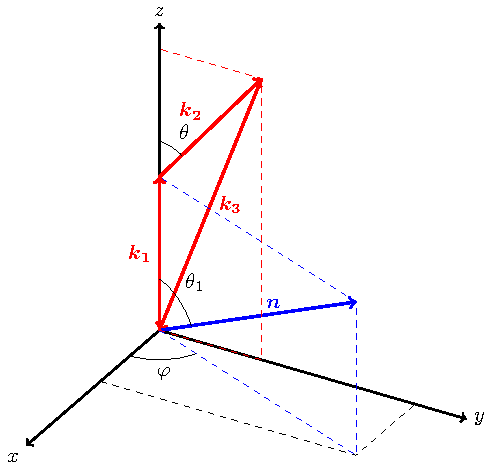
\includegraphics[width=0.6\linewidth]{fig/fig.pdf}
    \caption{Overview of the relevant vectors and angles for the Fourier-space bispectrum. \label{fig:geometry_overview1} }
\end{figure}       
Then we have $Y_{\ell m}(\mu_1,\varphi)$, so that we can write $B_g =\sum_{\ell m} B_{\ell m}Y_{\ell m}(\mu_1,\varphi)$. The leading relativistic terms we consider here generate odd-power multipoles up to $\ell=7$, and the full expression generates even and odd multipoles up to $\ell=8$-- see Chapter~\ref{chapter:multipoles}. 
Different powers of $(\i\mu_1)$ and $(\i\mu_2)$ contribute to the dipole as follows, \todo{check this table}
\begin{align}
\arraycolsep=1.0pt\def\arraystretch{1}
\int\mathrm{d}\Omega (\i\mu_1)^a  (\i \mu_2)^b Y^*_{1 m} & = 
 \delta_{m,0}\frac{\i\sqrt{3\pi}}{15}\left[ \begin {array}{ccccc} 
 0&10\mu&0&-6\mu  &\\ 
10&0&-4{\mu}^{2}-2&0& \cdots\\ 
0&-6\,\mu&0&{\frac {12{
\mu}^{3}+18\mu}{7}}& \\ 
-6&0&{\frac {24
\,{\mu}^{2}+6}{7}}&0& \\
 &\vdots & & & \ddots
\end {array} \right] \nonumber \\
& +
\delta_{m,\pm1}\frac{\sqrt{6\pi}}{15}
 \left[ \begin {array}{ccccc} 0&-5&0&3&\\ 
 0&0&2\,\mu&0
& \cdots\\ 
0&1&0&-\frac{6{\mu}^{2}+3}{7}&\\ 
0&0
&-\frac{6}{7}\,\mu&0&\\
 &\vdots & & & \ddots
\end {array} \right] \sin\theta\,,
\label{dkjsncdjcnsk}
\end{align}
where each matrix element corresponds to a particular combination of $a,b$,
where the matrix indices run over the values $a=0\ldots6, b=0\ldots6$, with powers above 3 not written above; these are polynomials in $\mu$ up to order 6. From this we can read off the terms from $\mathcal{K}_\text{D}$ contribute to differing $m=0,\pm1$. In particular, if $i+j$ is even~-- i.e., the real part of the bispectrum~--  there is no contribution: only the imaginary terms, corresponding to $i+j$ odd, contribute. For the monopole, only $i+j$ even contribute. Therefore, at $\ord(\cH/k)$, \emph{the monopole of the bispectrum is the Newtonian part, while the dipole is purely from the relativistic corrections.  The presence of the dipole is therefore a `smoking gun' signal for the leading relativistic correction to the bispectrum.} At order $\ord((\cH/k)^{2})$, relativistic terms appear in the monopole, which were considered in \citet{Umeh:2016nuh,Jolicoeur:2017nyt,Jolicoeur:2017eyi,Jolicoeur:2018blf}.\\


\section{Squeezed, equilateral and flattened limits}

It is relatively straightforward to understand the type of dipole generated in different triangular configurations in our conventions. In particular, for the $\ord(\cH/k)$ relativistic dipole:
\begin{itemize}
\item The squeezed case is zero for $m=0$, and is non-zero for $m=\pm1$. We see this directly from \eqref{dkjsncdjcnsk}: with $\mu=-1$ the $m=0$ contribution is anti-symmetric in $i,j$ while $\mathcal{B}_{ij}$ is symmetric in this limit.
\item In the equilateral case, the dipole is zero (this is the case for all orders in $\cH/k$).
\item The flattened case ($k_1=k_2=k_3/2,\theta=0$) is zero for $m=\pm1$ (for all orders in $\cH/k$), but is non-zero for $m=0$. This can be seen directly from \eqref{dkjsncdjcnsk} with $\theta=0$.
\end{itemize}
%Geometrically, we can understand these by rotating the triangle about its centre with respect to $\bm n$. For the equilateral case, the symmetry of the triangle means that the dipole part cancels out. For the flattened case, where there is a vertex at the centre, an anti-symmetry occurs only parallel to $\bm n$, and cancels in the plane orthogonal. For the squeezed case, this is anti-symmetric both along and perpendicular to $\bm n$, so excites both $m=\pm1$. 
 
To show the equilateral case is zero is a lengthy calculation involving many cancellations.  Let us illustrate instead the squeezed case. We write $k_1=k_2=\sqrt{1+\varepsilon^2}k_S, k_3=2\ep k_S$.
In this case the triangle has small angle $2\ep$ and equal angles $\pi/2-\ep$, where the squeezed limit is $\ep\to0$. It is convenient to replace $(1,2,3)$ by $(S,-S,L)$.
Then to $O(\ep)$,
$%\bea
k_{-S}= k_{S}\,,~~k_L=2\ep k_S\,,~~  
\mu_{-S}=-\mu_S-2\ep\mu_L\,,
%\nonumber\\&&
\mu_L = -\sqrt{1-\mu_S^2}\,\cos\varphi - {\ep\mu_S}\,.
%\hat{\k}_2=-\hat{\k}_1-2\ep\,\hat{\k}_3 \\ &&
$% \label{mu}
%\eea
 ~In this limit, the permutations of the relativistic kernels become
\begin{align}
% {\cal K}^{(2)}_{\mathrm{D}}(\k_S,\k_{-S},\k_L) &=&0\\
& {\cal K}^{(2)}_{\mathrm{D}}(\k_L,\k_S,\k_{-S}) = \i {\cH}
{\bigg[- \frac{3}{2}\Omega_m b_1\mu_S \frac{k_S}{k_L^2}+ C f \frac{\mu_L}{k_L} }
\nonumber\\
& - \frac{3}{2} \Omega_m f\mu_S^3 \frac{k_S}{k_L^2} +\Big( \frac{3}{2} \Omega_m- Ef \Big) f\mu_S^2 \frac{\mu_L}{k_L}\bigg] 
\label{k2d1} 
% {\cal K}^{(2)}_{\mathrm{D}}(\k_{-S},\k_L,\k_S) &=&  {\cal K}^{(2)}_{\mathrm{D}}(\k_L,\k_S,\k_{-S})\Big|_{\mu_S\to \roy{\mu_{-S}}}  \label{k2d2}
\end{align}
and $ {\cal K}^{(2)}_{\mathrm{D}}(\k_{-S},\k_L,\k_S) =  {\cal K}^{(2)}_{\mathrm{D}}(\k_L,\k_S,\k_{-S})\big|_{\mu_S\to {\mu_{-S}}}$ while ${\cal K}^{(2)}_{\mathrm{D}}(\k_S,\k_{-S},\k_L) =0$. 
In the squeezed limit of the cyclic sum~\eqref{eq:fsbispdef}, the terms $ {\cal K}^{(2)}(\k_L,\k_S,\k_{-S})$ and  ${\cal K}^{(2)}(\k_{-S},\k_L,\k_S)$ appear only in the form ${\cal K}^{(2)}(\k_L,\k_S,\k_{-S})+{\cal K}^{(2)}(\k_{-S},\k_L,\k_S)$. This sum regularises
the divergent $k_S/k_L=(2\ep)^{-1}$ and $k_S/k_L^2=(2\ep k_L)^{-1}$ terms.  We obtain the bispectrum in the squeezed limit,


\begin{align}
&B_{g}^{\mathrm{sq}} = b_{1S}b_{1L}b_{SL}\, P_LP_S+\i b_{1S}\Big\{b_{SL}f A + {\frac{3}{2}} \Omega_m b_{1S}b_{1L} 
\nonumber\\
&+2b_{1L}f C+ b_{1L}\mu_S^2\Big[{\frac{3}{2}}\Omega_m- Ef \Big] \Big\}P_LP_S\,\mu_L \frac{\cH}{k_L} \,,\label{bgd}
\end{align}


where $P_{S,L}=P(k_{S,L})$, $b_{1S,L}\equiv  b_1+f\mu_{S,L}^2$ and
\begin{align}
% \,, \label{b1sl}~~
b_{SL} \equiv 2b_2+ \frac{43}{21}b_1 - \frac{4}{21}
%\nonumber\\&&
+\Big(2b_1+ \frac{5}{7}\Big)f\mu_S^2%+b_1f\mu_L^2+{f^2}\mu_S^2\mu_L^2 
+f\mu_L^2 b_{1S}
\,. \nonumber\label{bsl}
\end{align}
%Note that we can neglect the $P(k_S)^2$ term relative to the $P(k_L)P(k_S)$ term in $B_{g {\mathrm{N}}}^{\rm sq}$.
Note that only the first term in the squeezed bispectrum comes from the Newtonian limit. 

The type of dipole extracted from this term is seen as follows. To this order we can write $\mu_{S}^2=\mu_{S}\mu_{-S}$. Then,  since $\mu_L=-2(\mu_S+\mu_{-S})/
\varepsilon$, we see that the $m=0$ term is zero because $B_{g {\mathrm{D}}}^{\mathrm{sq}}$ is symmetric in $\mu_{S}^i\mu_{-S}^j$ under $i\leftrightarrow j$, while the $m=0$ term is antisymmetric in~\eqref{dkjsncdjcnsk}. This leaves just the $m=\pm1$ contribution in \eqref{dkjsncdjcnsk}.




\begin{figure}%[htbp]
\begin{center}
%\includegraphics[width=\columnwidth]{flattened-squeezed-02}
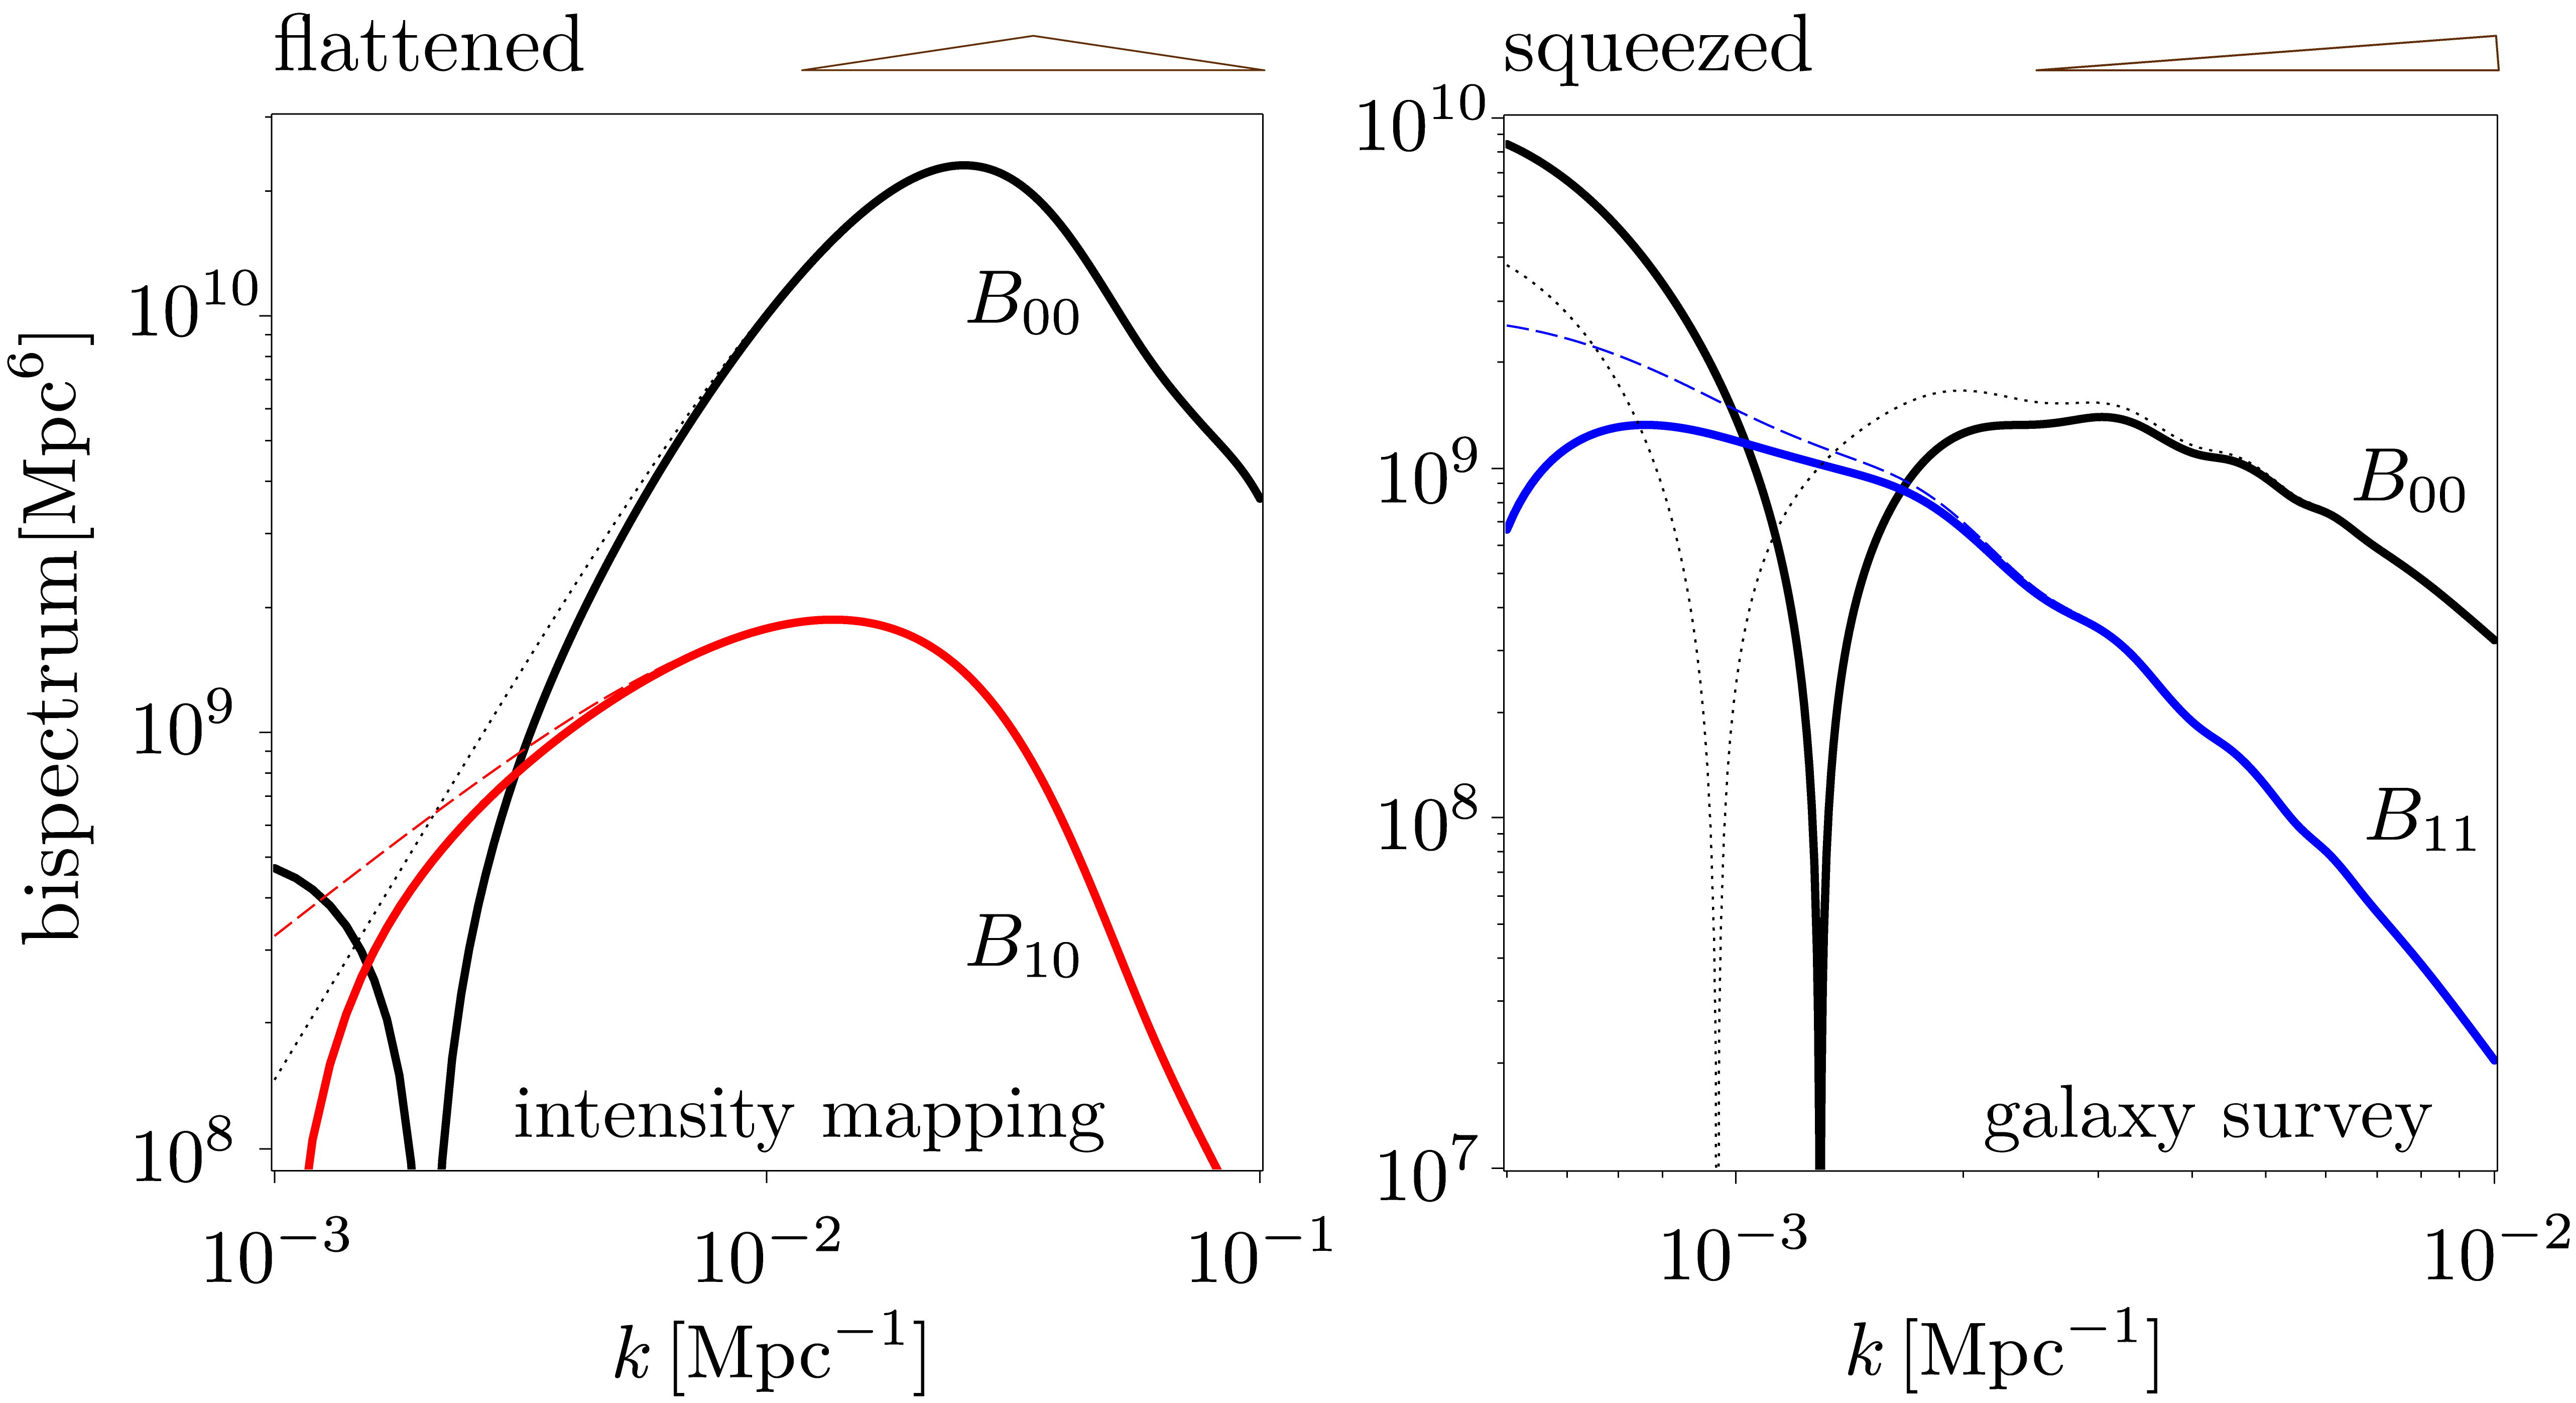
\includegraphics[width=\columnwidth]{fig/figuresv2-02}
\caption{ The absolute value of the bispectrum dipole at $z=1$  as a function of triangle size, in the flattened (Left, $\theta=2^\circ$, for intensity mapping bias) and squeezed (Right, $\theta=178^\circ$, for Euclid-like bias) configurations, with $k_3$ as the horizontal axis. Red is the $m=0$ part and blue is $m=\pm1$. Dashed (and dotted) lines show up to the $\ord(\cH/k)$ terms considered analytically here, while solid lines indicate larger-scale contributions. For reference the monopole is in black, with the dotted line the Newtonian part.  (The zero-crossing in the monopole for the squeezed case is a result of the tidal bias.)}
\label{snakcjnsdlkcans}
\end{center}
\end{figure}

\begin{figure}%[htbp]
\begin{center}
%\includegraphics[width=\columnwidth]{shapes-01}
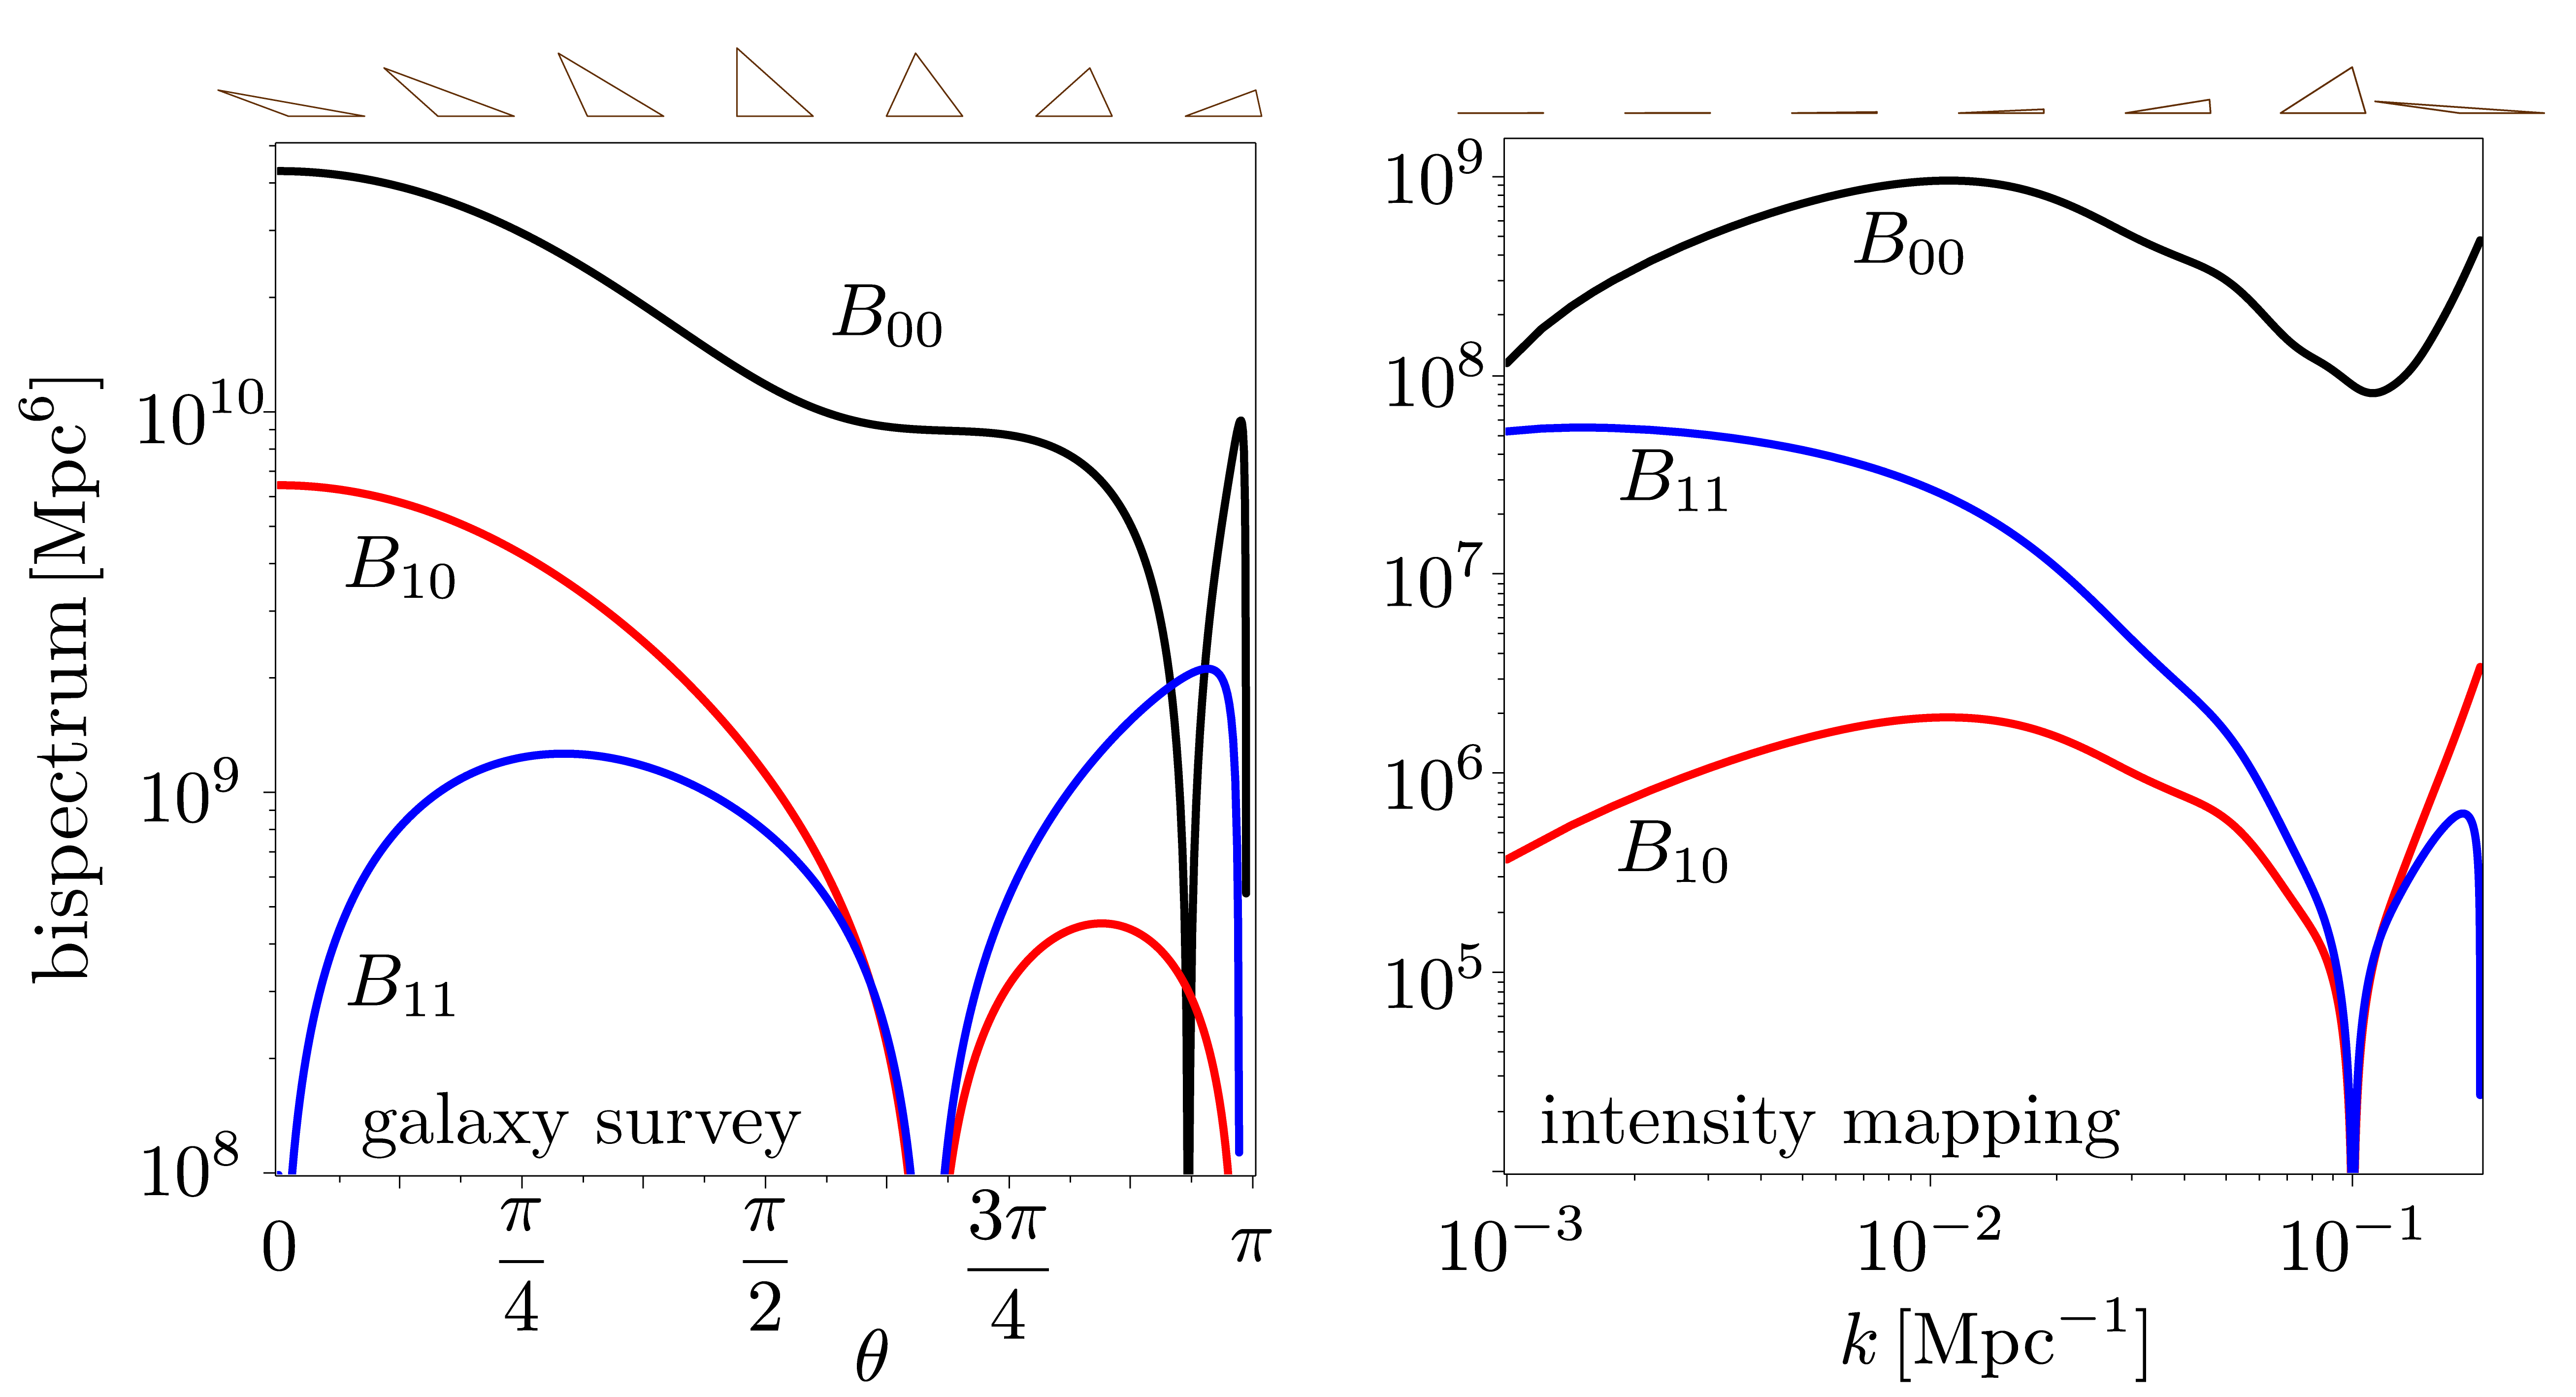
\includegraphics[width=\columnwidth]{fig/figuresv2-01}
\caption{ (Left) We show the dipoles as a function of $\theta$ with a bias appropriate for a Euclid-like survey, for $k_1=k_2=0.01$\,Mpc$^{-1}$. The left of the plot corresponds to the flattened case where the $m=0$ (red) dipole reaches 10\% of the monopole.  (Right) We show the IM signal with $k_1=k_2=0.1$\,Mpc$^{-1}$ versus the long mode $k_3$. Except for very long modes $\theta\approx\pi$, our $\ord(\cH/k)$ truncation is a very good approximation in these examples. }
\label{sankcjnakjdcs}
\end{center}
\end{figure}
 


\section{The dipole in intensity mapping and galaxy surveys}

We now consider the amplitude of the dipole relevant for upcoming galaxy surveys, which have different bias parameters. We consider two different types of survey: an SKA intensity mapping of 21\,cm radio emission, as well as a Euclid-like optical/infrared spectroscopic survey.
An intensity map of the 21cm emission of neutral hydrogen (HI) in the post-reionization Universe records the total emission in galaxies containing HI, without detecting individual galaxies. There is an equivalence between the brightness temperature contrast and number count contrast~\citep{Umeh:2015gza}. \todo{check the bias params, and provide expressions} For IM we use the bias parameters at $z=1$, 
$b_1 = 0.856, b_2 = -0.321, b_1' = -0.5\times10^{-4}, b_e = -0.5, b_e'=0, s = 2/5$~\citep{Fonseca:2018hsu,Umeh:2015gza}
while for the spectroscopic survey we use 
$ b_1 = 1.3,b_2 = -0.74, b_1' = -1.6\times10^{-4},  b_e = -4, b_e' = 0, s = -0.95$~\citep{Camera:2018jys,Yankelevich:2018uaz}.
For intensity mapping, $ \partial b_1/\partial \ln L =0$ and we assume it is zero for simplicity for the spectroscopic survey. We use a LCDM model with standard parameters $\Omega_m=0.314, h=0.67, f_\text{baryon}=0.157, n_s=0.968$. Plots are presented using linear power spectra generated using CAMB~\citep{Lewis:1999bs}.

In Fig.~\eqref{snakcjnsdlkcans} \todo{move figures into section} we show how changing the scale of a fixed triangle changes the amplitude of the dipole, with reference to the monopole. In the flattened case with $m=0$ we see the signal peaks for triangles below the equality scale, while for squeezed shapes, with $m=\pm1$, the signal is smaller, and peaks when the long mode approaches the Hubble scale. 
In Fig.~\eqref{sankcjnakjdcs} we change the shape with fixed $k_1=k_2$ for both galaxy and IM surveys. We confirm our analytical results that the equilateral limit is zero, as well as the other limits. For triangles between right-angle and flattened the dipole is more than 10\% of the monopole, and the signal is largest in the flattened case~-- except in the extreme squeezed limit (not shown). 


\section{Conclusions}

We have shown for the first time that the relativistic galaxy bispectrum has a leading correction which is a local dipole with respect to the observers line of sight. In contrast to the power spectrum, this dipole exists even for a single tracer. We have shown analytically how the dipole is generated for the leading terms, and numerically we have included all local contributions, which show up above the equality scale. We have neglected integrated terms which will also contribute to the dipole, but their inclusion in a Fourier space bispectrum is non-trivial. Local relativistic corrections will induce all multipoles up to $\ell=8$ at every $m$, in contrast to the Newtonian case which only induces even $\ell=0,2,4$. We will investigate these new multipoles in a forthcoming publication. 

We have shown that this dipole is large with respect to the monopole in both the flattened and squeezed limits, which excite different orders of the dipole orientation $m$.  We have shown that even on equality scales it is about 10\% of the monopole at $z=1$ for flattened shapes which have the largest amplitude. In more squeezed cases where the short mode is $\sim10$\,Mpc the dipole can also be a large part of the IM signal. Furthermore, although we have only considered Gaussian initial conditions here, the dipole will be unaffected by non-Gaussianity at leading order because these corrections start at $\ord((\cH/k)^2)$, making our predictions relatively robust to this. This implies that the dipole of the bispectrum is a unique signature of general relativity on cosmological scales, and therefore offers a new observational window onto modifications of general relativity. 





%
\chapter{Detectability in Spectroscopic Surveys}
\label{chapter:snreuclid}

SNR calc for Euclid-like survey
%
\chapter{Detectability in IM Surveys}
\label{chapter:snrska}


%
%
%---------------------------
%
%
\section{21cm intensity mapping surveys}
%
Some blah blah about intensity mapping 
%
\section{Introduction}
%

}
%
%
%---------------------------------------------
%
%
\section{Relativistic effects in the 21cm intensity bispectrum}
%

%
%-----------------------------------------------------------
%
%
\section{Relativistic signal-to-noise ratio}
%
{The signal-to-noise ratio for a bispectrum in the Gaussian case is given by 
$\mathrm{SNR}^2 = {B^2 / \mathrm{Var}(B)}$, where the variance includes cosmic variance as well as noise.
The relativistic part of the bispectrum at leading order is extracted as the imaginary part of the estimator for the bispectrum. For the variance, we use the fact that it is unaffected by relativistic corrections at leading order: $\mathrm{Var}(B_{\hi})= \mathrm{Var}(B_{\mathrm N})+O(\cH^2/k^2)$, as shown in \cite{Maartens:2019yhx}.}
%
The bispectrum in each $z$-bin has 5 independent degrees of freedom, which we choose as the 3 sides $k_a$ of the closed triangle and 2 angles $(\theta_1=\cos^{-1}\mu_1,\varphi)$
that define the orientation of the triangle.
The relativistic SNR per $z$-bin is then given by  \cite{Maartens:2019yhx}
\begin{equation}
{{\mathrm{SNR}}(z)^2 =
\sum_{k_a,\mu_1,\varphi}\,\frac{B_{\mathrm D}(z, k_{a},  \mu_{1},\varphi) \,B_{\mathrm D}^*(z, k_{a},  \mu_{1},\varphi)}{{\mathrm Var} [{B_{\mathrm N}}(z, k_a,\mu_{1},\varphi)]}\,,} \label{e2.2_0}
\end{equation}
where we isolated the imaginary part, 
and the cumulative SNR is defined by
\begin{equation}
{{\mathrm SNR}(\leq z)^2 =
\sum_{z'}\,{\mathrm SNR}(z')^2\,.} \label{csnr_d2ß}
\end{equation}
The total SNR is  $\mathrm{SNR}(\le z_\mathrm{max})$.

The variance is estimated as 
\begin{equation}
\!\!\!{\mathrm{Var} [{B_{\mathrm N}}(z, k_a,\mu_{1},\varphi)]}
=\frac{s_B\,\pi\, k_{\mathrm f}(z)^3}{k_1k_2k_3 (\Delta k)^3}\,\frac{{4\pi}}{ \Delta \mu_1 \Delta \varphi} \,
\tilde{P}_{\hi}(z,k_{1},\mu_{1})\,\tilde{P}_{\hi}(z,k_{2},\mu_{2}) \,\tilde{P}_{\hi}(z,k_{3},\mu_{3})\,.
\label{e2.7}
\end{equation}
Here
\begin{equation}
\tilde{P}_{\hi}(z, k, \mu) = P_{\hi}(z, k, \mu) + P_\mathrm{noise}(z,k,\mu)\,, \label{e2.4}
\end{equation}
where the HI power spectrum is Newtonian at leading order: $P_{\hi}= P_{\hi} +O(\cH^2/k^2)$, with
\begin{equation}
P_{\mathrm N}(z, k, \mu) = \big[b_{1}(z)+f(z)\mu^{2}\big]^{2}P_{\mathrm m}(z,k)\,.\label{e2.5_1}
\end{equation}
In \eqref{e2.7}, the multiplicity constant $s_B=6, 2, 1$ for equilateral, isosceles, and non-isosceles triangles,  and $\Delta k,\Delta \mu_1,  \Delta \varphi$ are bin widths. We follow \citep{Karagiannis:2018jdt,Maartens:2019yhx} and choose the step lengths as
\begin{equation}
\Delta z = 0.1\,, \quad \Delta \mu = 0.04\,, \quad {\Delta\varphi=\pi/25}\,, \quad \Delta k(z) = k_{\mathrm{f}}(z)\,.\label{e4.1} 
\end{equation} 
The fundamental mode $k_{\mathrm{f}}$ is an estimate of  the minimum wavenumber included in the survey, and is determined in each redshift bin  by the comoving volume of the bin centred at $z$:
\begin{equation}
k_{\mathrm{f}}(z) = \frac{2\pi}{V(z)^{1/3}} \quad \mbox{with} \quad V(z) = \frac{4\pi}{3}f_{\mathrm{sky}} \big[r(z+{\Delta z}/{2})^{3} - r(z-{\Delta z}/{2})^{3} \big] \,.\label{e2.8}
\end{equation}
Here $f_{\mathrm{sky}}=\Omega_\mathrm{sky}/4\pi$ is the sky fraction covered by the survey.
%
%
%-----------------------------------
%
%
\subsection{Nonlinearity}
%
The tree-level bispectrum is a perturbative model. In order to avoid scales where dark matter clustering becomes nonperturbative, we impose a maximum scale \cite{Maartens:2019yhx}
\begin{equation} \label{eq:snrkmax}
k_{\mathrm{max}}(z) = 0.1h\,(1+z)^{2/(2+n_s)}~\mathrm{Mpc}^{-1}\,.
\end{equation}
However, applying this cut-off still includes nonperturbative RSD effects, i.e. the fingers-of-god damping. In order to take account of this, we follow \cite{Karagiannis:2018jdt,Yankelevich:2018uaz,Maartens:2019yhx} and use the following phenomenological model of the damping of redshift-space clustering due to nonlinear velocities:
\begin{align}
 P_{\hi}(k,\mu,z) & ~\to~   \exp\Big[-\frac{1}{2}{k^2\mu^2\,{\sigma_{P}(z)}^{2}}\Big]\,P_{\hi}(k,\mu,z)
 \,, \label{e2.10}\\
 B_{\hi}(k_a,\mu_a,z) & ~\to~  \exp\Big[-\frac{1}{2}{\left( k_{1}^{2}\mu_{1}^{2}+k_{2}^{2}\mu_{2}^{2}+k_{3}^{2}\mu_{3}^{2}\right){\sigma_{B}(z)}^{2}}\Big]\,B_{\hi}(k_a,\mu_a,z)
 \,. \label{e2.11}
\end{align}
Damping is effective for $k\gtrsim \sqrt{2}/\sigma_P$ for the power spectrum and  $k\gtrsim \sqrt{2}/\sigma_B$ for the bispectrum.
In this model, the damping parameters $\sigma_P$ and $\sigma_B$ are  to be determined by data or simulations.
We use a model for the power spectrum damping parameter based on HI simulations \cite{Sarkar:2019ojl}:
\begin{equation}
\sigma_{P}(z) = 11h\big(1+z\big)^{-1.9}\exp{\big[-(z/11)^{2}\big]}~~h^{-1}\,\mathrm{Mpc}\,. \label{e2.12}  \\
\end{equation}
We are not aware of any simulation-based expression for $\sigma_B$, and we therefore take $\sigma_B=\sigma_P$ as a first approximation. The
effect of increasing $\sigma_B$ is discussed in Section ref sec5.

A further source of nonlinearity on weakly nonlinear scales that contributes to the bispectrum variance  is the non-Gaussian effect due to mode coupling. We follow \cite{Karagiannis:2018jdt,Maartens:2019yhx} and  take account of this using the simple model developed in \cite{Chan:2016ehg}, which modifies the variance as follows: 
\begin{equation}
\mathrm{Var} [{B_{\mathrm N}}(\k_a)]  \to  \mathrm{Var}  [{B_{\mathrm N}}(\k_a)] \left[1+  
\frac{\delta\tilde{P}_{\mathrm N}(\k_1)}{\tilde{P}_{\mathrm N}(\k_1)} + \frac{\delta\tilde{P}_{\mathrm N}(\k_2)}{\tilde{P}_{\mathrm N}(\k_2)} + \frac{\delta\tilde{P}_{\mathrm N}(\k_3)}{\tilde{P}_{\mathrm N}(\k_3)}\right]  .
 \label{eq:e2.14}
\end{equation}
 Here the redshift dependence  has been dropped for brevity, and
\begin{align}
\delta\tilde{P}_{\mathrm N}(\k) & = \tilde{P}_{\mathrm N}^{\nl}(\k) - \tilde{P}_{\mathrm N}(\k)\,, 
\label{eq:e2.15}\\
\tilde{P}^{\nl}_{\mathrm N}(\k) =& \big(b_{1}+f\mu^2\big)^2P^{\nl}_{\mathrm m}(k)+P_\mathrm{noise}(\k)\,,\label{e2.15_1}
\end{align}
where $\tilde{P}_{\mathrm N}={P}_{\mathrm N}+P_\mathrm{noise}$ and
$P^{\nl}_{\mathrm m}$ is the nonlinear matter power spectrum computed in CLASS with a modified Halofit emulator.
%
%
\subsection{Effects of foregrounds}
%
\subsection{Maximum and minimum scales probed}
%
\subsection{Instrumental noise}
%
\subsection{Future HI intensity mapping surveys}
%
We consider surveys proposed for the following dish arrays:
\begin{itemize}
\item 
SD mode:  MeerKAT, 
SKA1-MID.
\item
IF\ mode: HIRAX,
PUMA (Petite). 
\end{itemize}
The survey specifications are given in Table~\ref{tab:tab1}, {based on~\cite{Santos:2017qgq, Bacon:2018dui, Slosar:2019jwd,Karagiannis:2019jjx,Castorina:2020zhz}}. {Limiting wavenumbers for large wavelengths  are shown for these surveys in Figure \ref{figmin}: the
fundamental wavenumber \eqref{e2.8}, the minimum radial wavenumber \eqref{kfgpar} from foreground cleaning and the IF-mode minimum wavenumber \eqref{kifmin}.}
%\vspace{-0.5cm}

\begin{table}[ht]
\centering
\caption{\label{tab:tab1} {HI intensity mapping survey specifications. 
(For *, see Appendix REF APPENDIX 2 OF IM)}} 
\vspace*{0.2cm}
\begin{tabular}{|lccccccc|} \hline
Survey & Redshift range & $f_\mathrm{sky}$ & $t_{\mathrm{tot}}$  & $T_{\mathrm{d}}$ & $D_\mathrm{d}$ & $N_\mathrm{d}$ & {$D_\mathrm{max}$} \\
&  & & [$10^{3}$ hr] & [K]  & [m] & & {[m]} \\
\hline\hline 
MeerKAT L Band   & 0.10--0.58 & 0.10 & 4  & * & 13.5 & 64 & -- \\
MeerKAT UHF Band & 0.40--1.45 & 0.10 & 4  & * & 13.5 & 64  & --  \\
SKA1-MID Band 1  & 0.35--3.05 & 0.48 & 10 & * & 15.0 & 197  & --  \\
SKA1-MID Band 2  & 0.10--0.49 & 0.48 & 10 & * & 15.0 & 197  & --  \\
HIRAX            & 0.75--2.00 & 0.36 & 10 & 50 & 6.0  & 1024  & {270}\\
PUMA (Petite)    & 2.00--6.00 & 0.50 & 40 & 50 & 6.0  & 5000 & {600} \\
\hline
\end{tabular}
\end{table}

\vspace*{-0.5cm}
\begin{table}[ht]
\centering
\caption{\label{tab2} {Parameters in \eqref{e3.4}} (from~\cite{Ansari:2018ury}).} 
\vspace*{0.2cm}
\begin{tabular}{|lcccccl|} \hline
Survey & $a$ & $b$ & $c$  & $d$ & $e$ & $N_\mathrm{s}$  \\ \hline\hline 
HIRAX & 0.4847 & $-0.3300$ & 1.3157 & 1.5974 & 6.8390 & 32  \\
PUMA (Petite) & 0.5698 & $-0.5274$ & 0.8358 & 1.6635 & 7.3177 & {100} \\
\hline
\end{tabular}
\end{table}

For the system temperature, we use the results of measurements and simulations for MeerKAT and SKA1-MID, given in Appendix REF APP IM. For HIRAX and PUMA, we use the fit \eqref{e2.25}. 


In IF mode, HIRAX is assumed to be a square-packed array, while PUMA is taken as hexagonal-packed in a circular area, {with 50\% fill factor}. We follow~\cite{Karagiannis:2019jjx} and use the fitting formula from~\cite{Ansari:2018ury} for the baseline density of such arrays:
\begin{equation}
n_\mathrm{b}^\mathrm{phys}(L) = \left( \frac{N_\mathrm{s}}{D_\mathrm{d}}\right)^2\,\frac{a+b\big(L/L_\mathrm{s}\big)}{1+c\big(L/L_\mathrm{s}\big)^{d}}\,\exp{\big[-(L/L_\mathrm{s})^{e}\big]}\,, \label{e3.4}
\end{equation}
where  $L_\mathrm{s} =N_\mathrm{s}D_\mathrm{d}$ and $N_\mathrm{s}^2 = N_\mathrm{d}$.
The  parameters in \eqref{e3.4} are given in Table \ref{tab2}, {and $n_\mathrm{b}^\mathrm{phys}(L)$ is shown in Figure~\ref{nbphys}.
\begin{figure}%[h]
%\vspace*{-0.5cm}
\centering
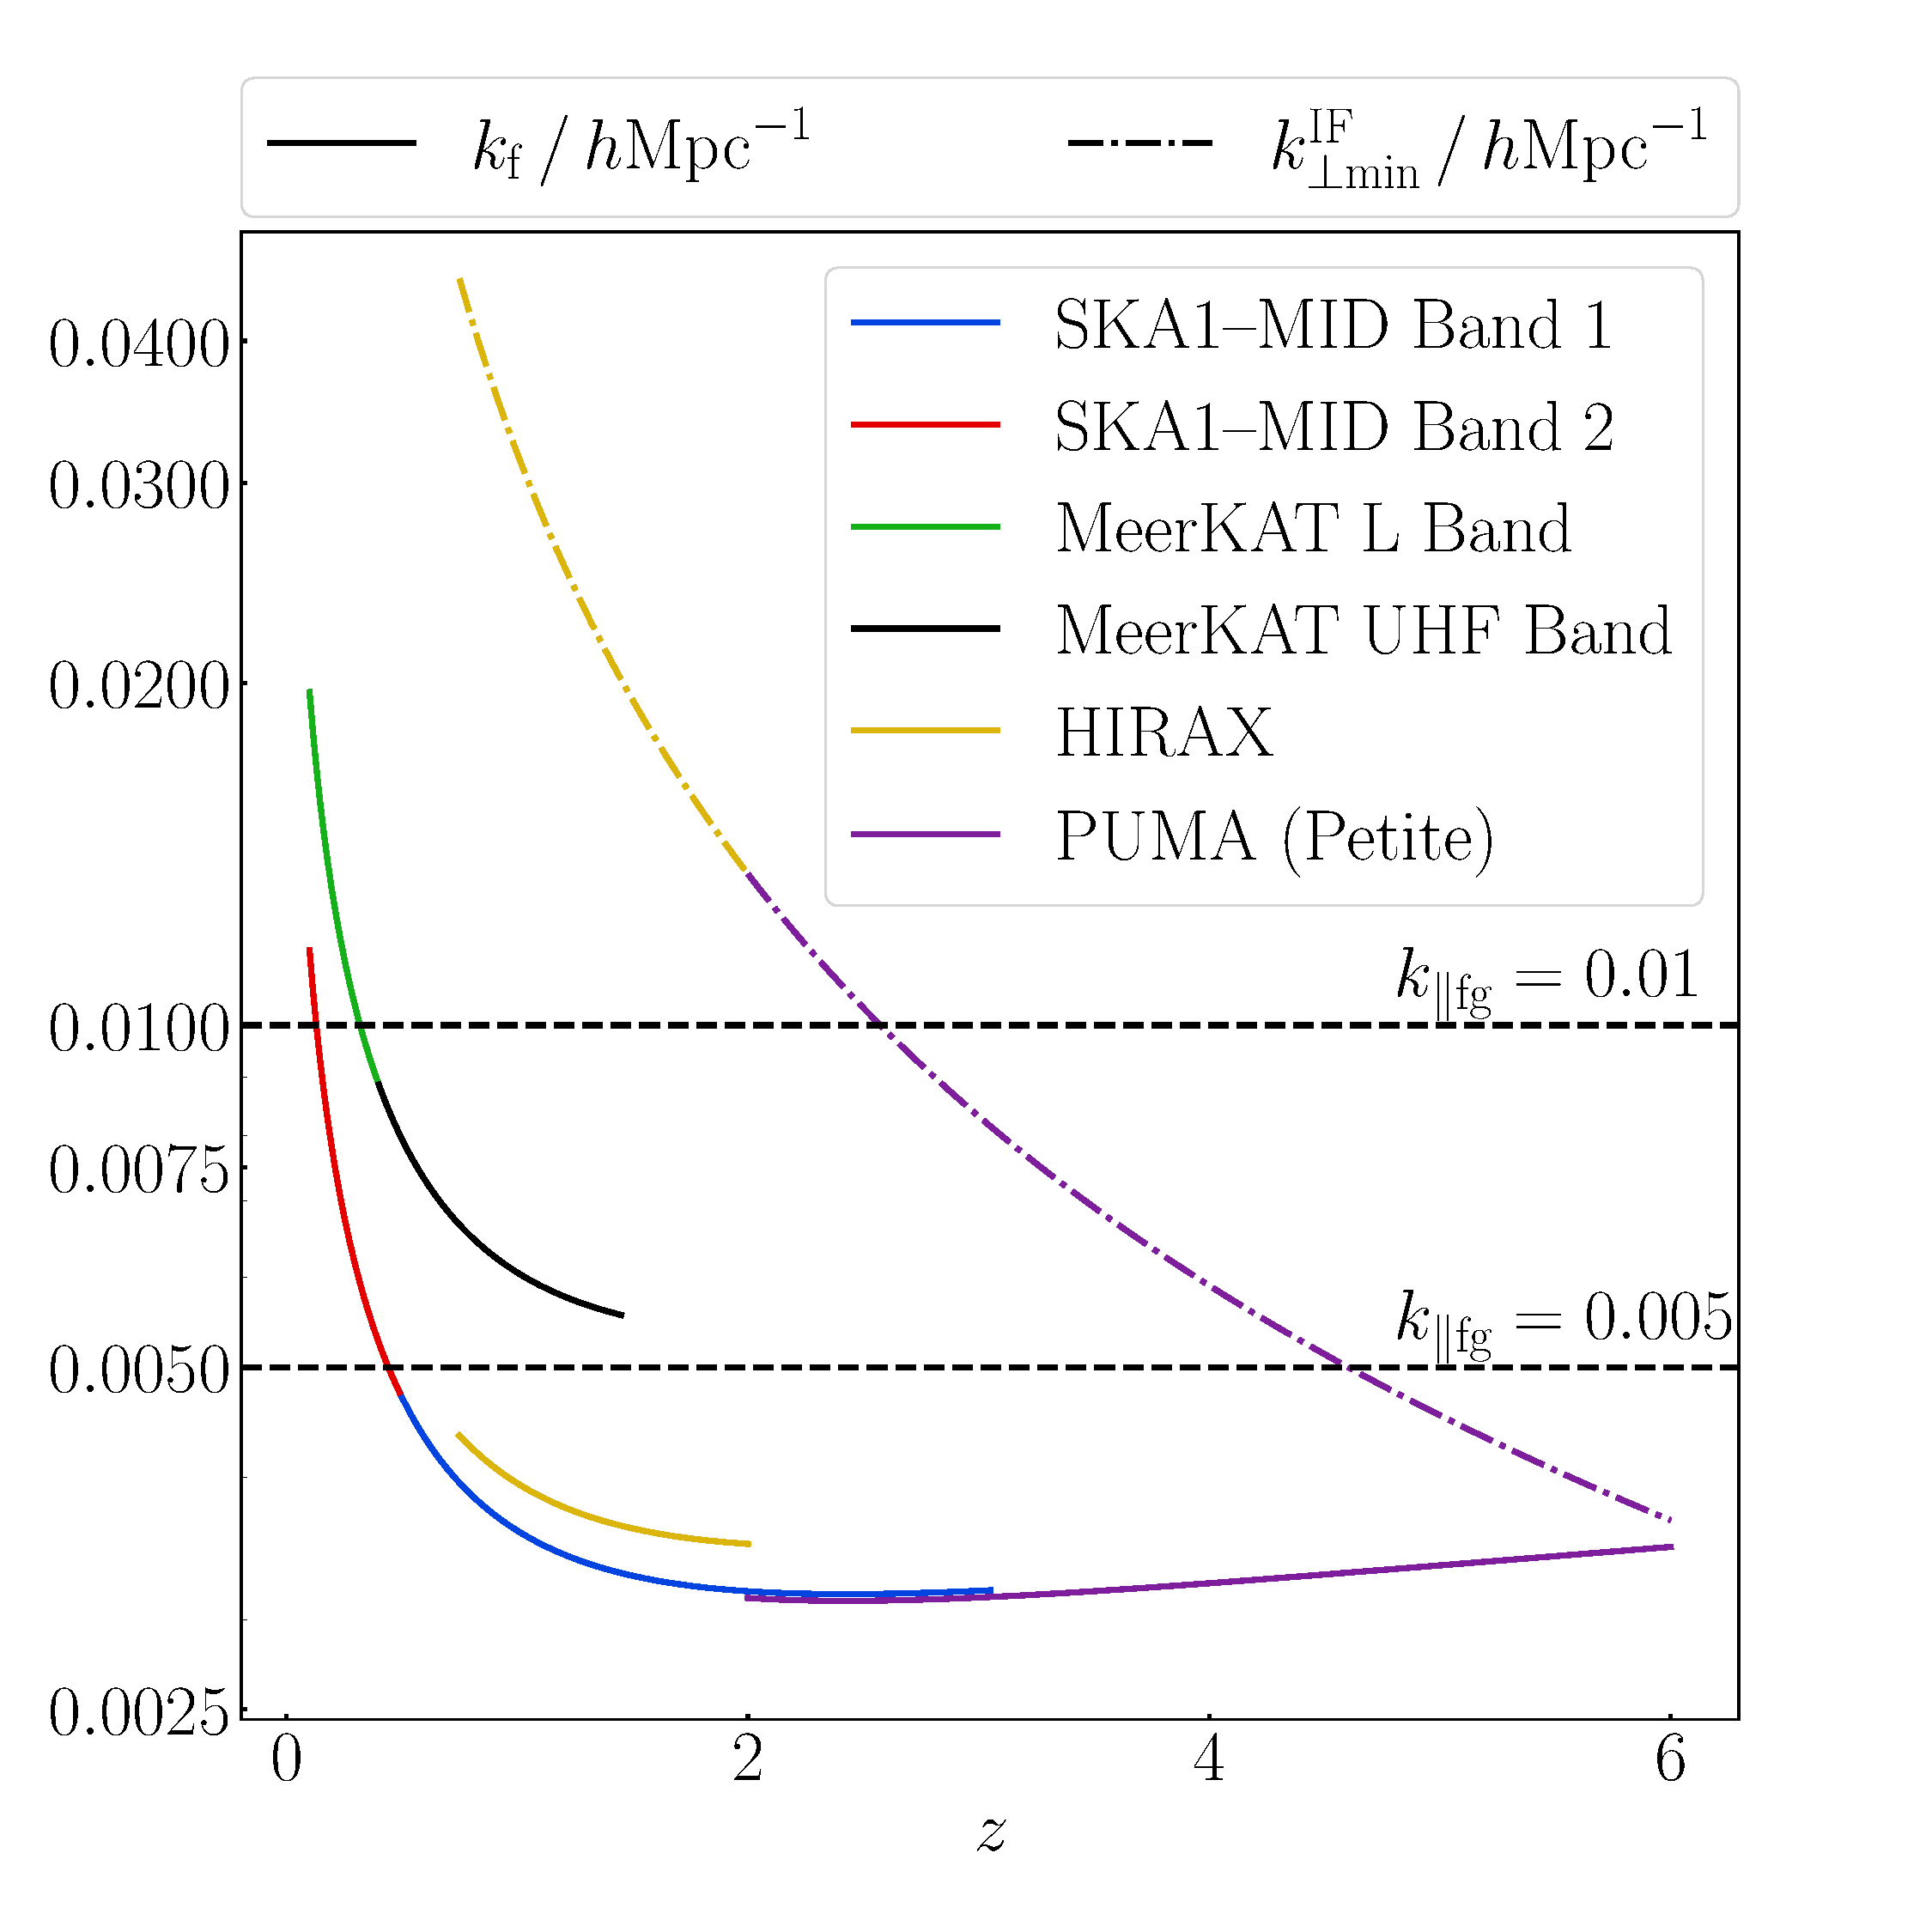
\includegraphics[width=.49\textwidth]{fig/k}
%\vspace*{-0.5cm}
\caption{{Minimum wavenumbers for the surveys, where $k$ is subject to \eqref{kmin} (SD) or \eqref{kminif} (IF).}}\label{figmin}
\end{figure}

%\vspace*{-0.5cm}
\begin{figure}[ht]
\centering
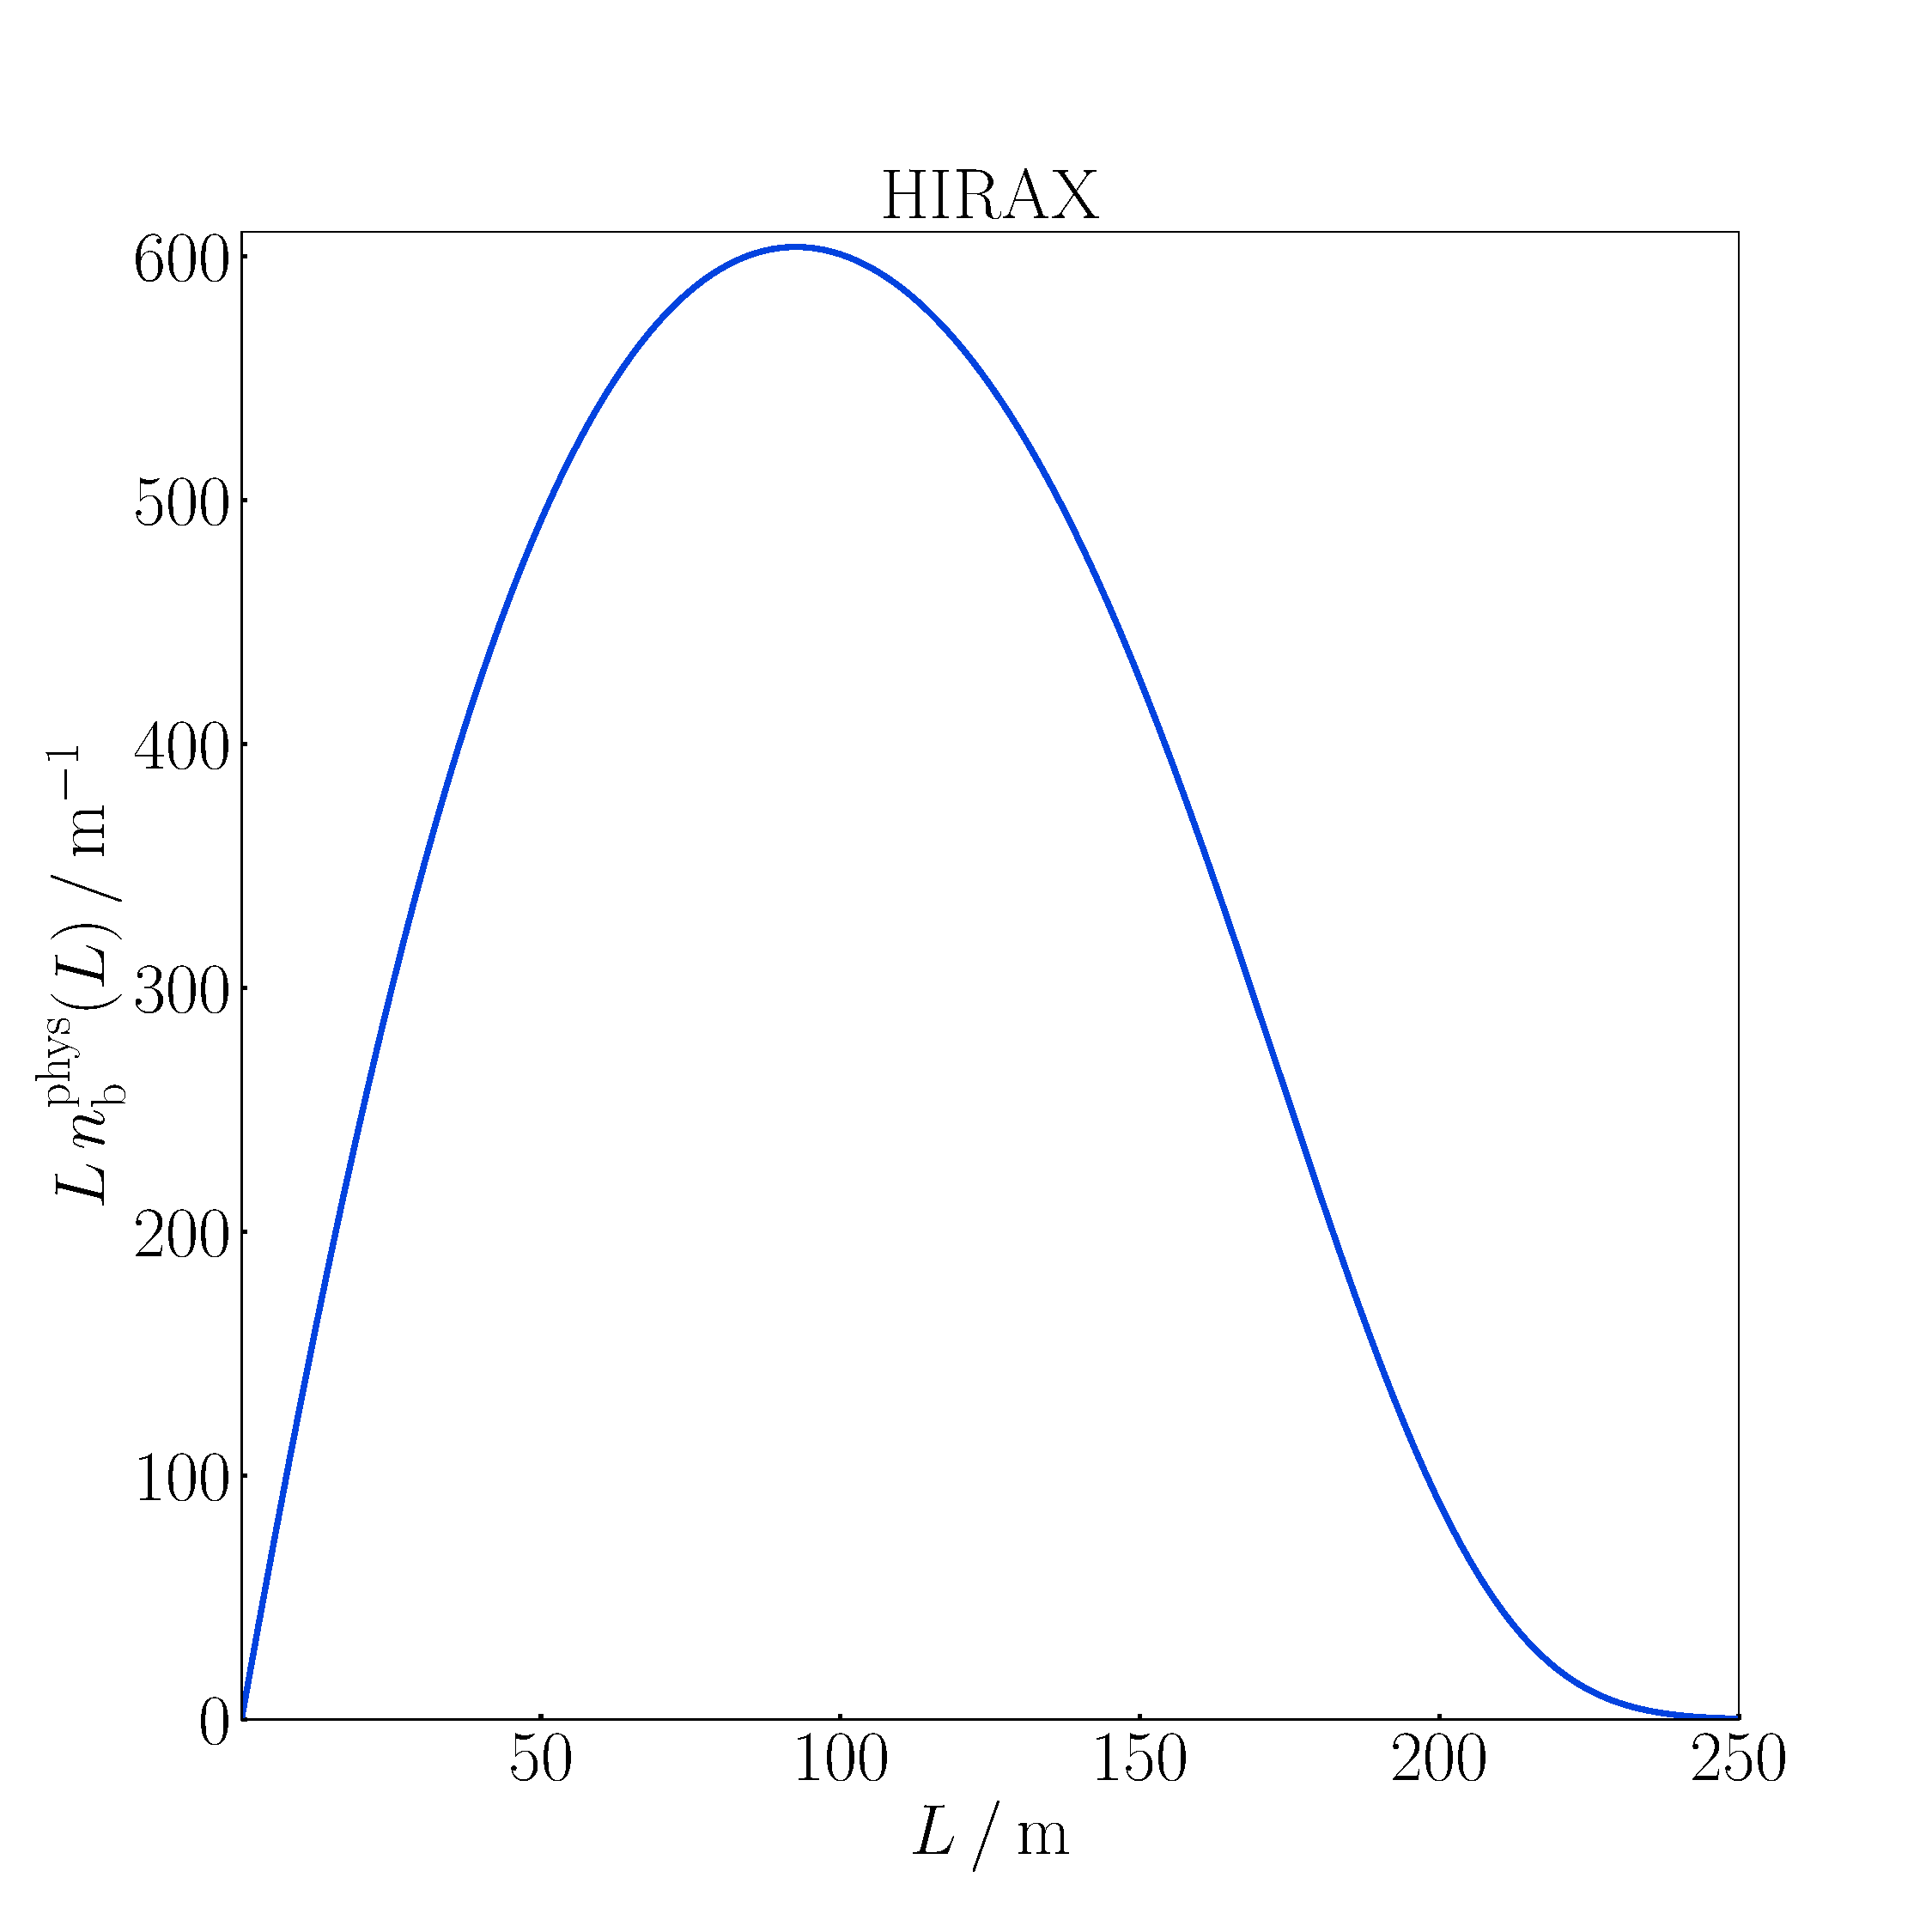
\includegraphics[width=.49\textwidth]{fig/nbHIRAX}
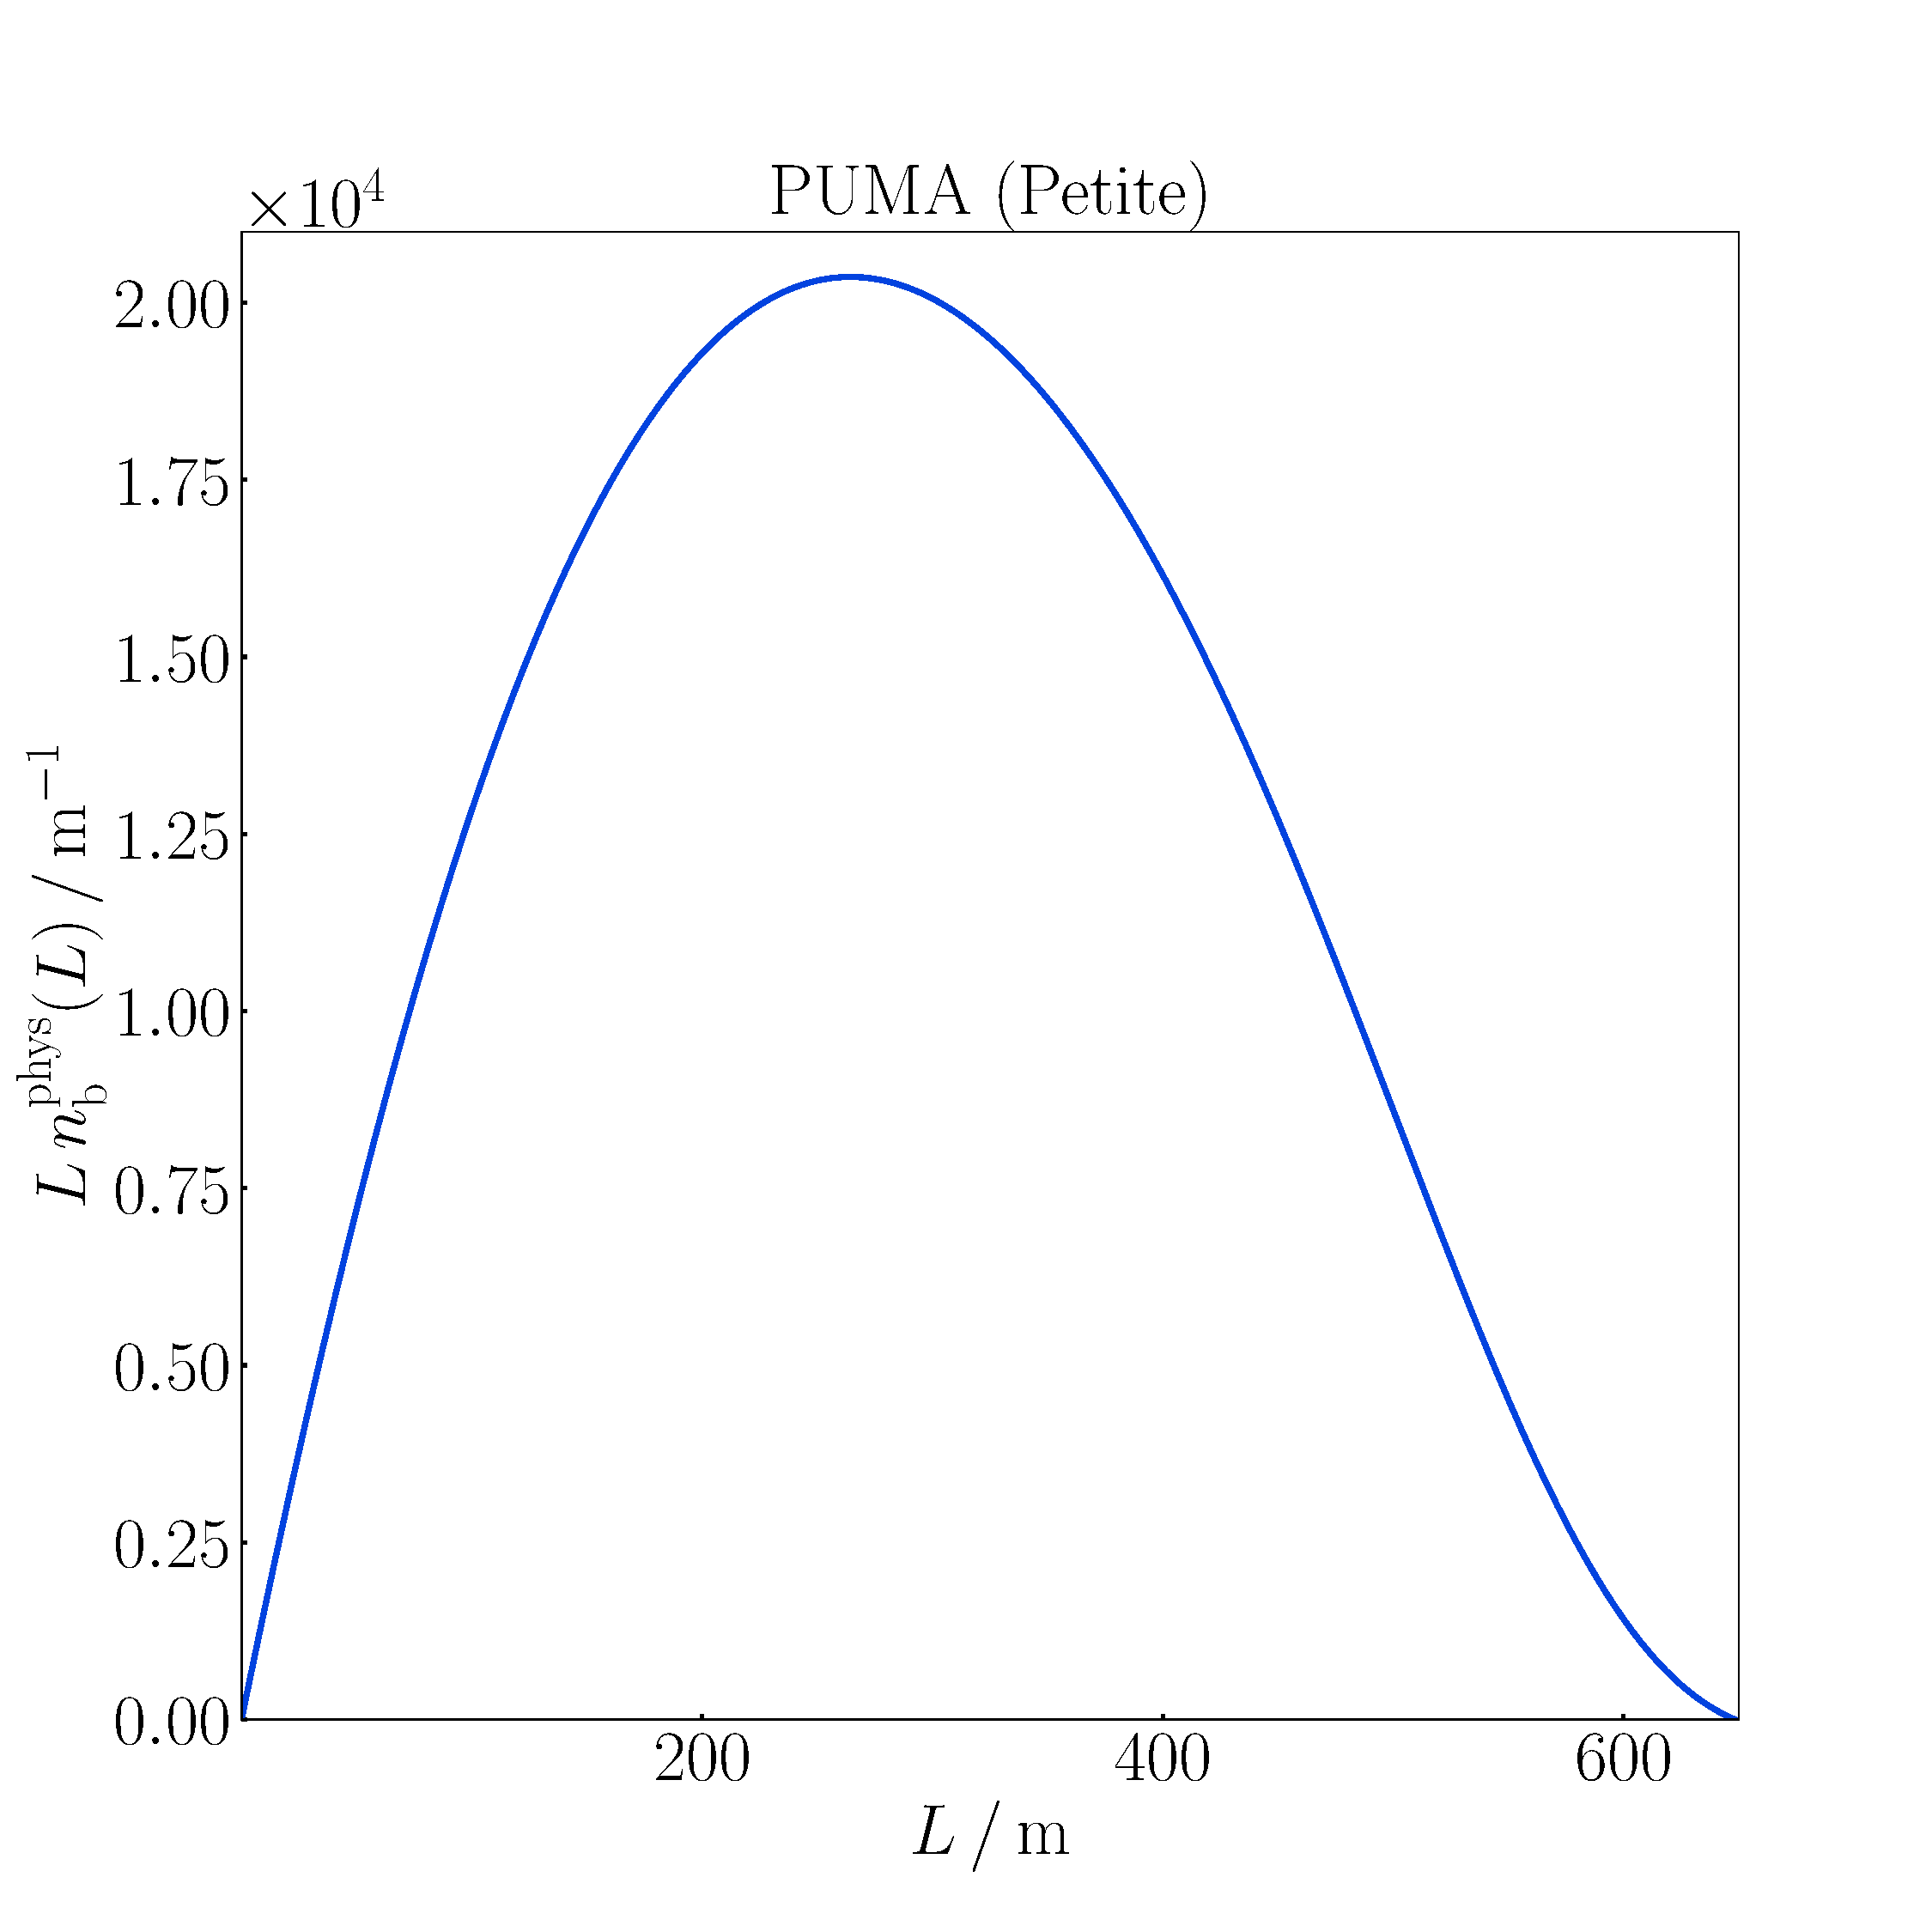
\includegraphics[width=.49\textwidth]{fig/nbPUMAPetite}
\vspace*{-0.5cm}
\caption{Physical baseline density models for HIRAX (left) and PUMA (right).}\label{nbphys}
\end{figure}
%\vspace*{-0.5cm}
\begin{figure}[!ht]
\centering
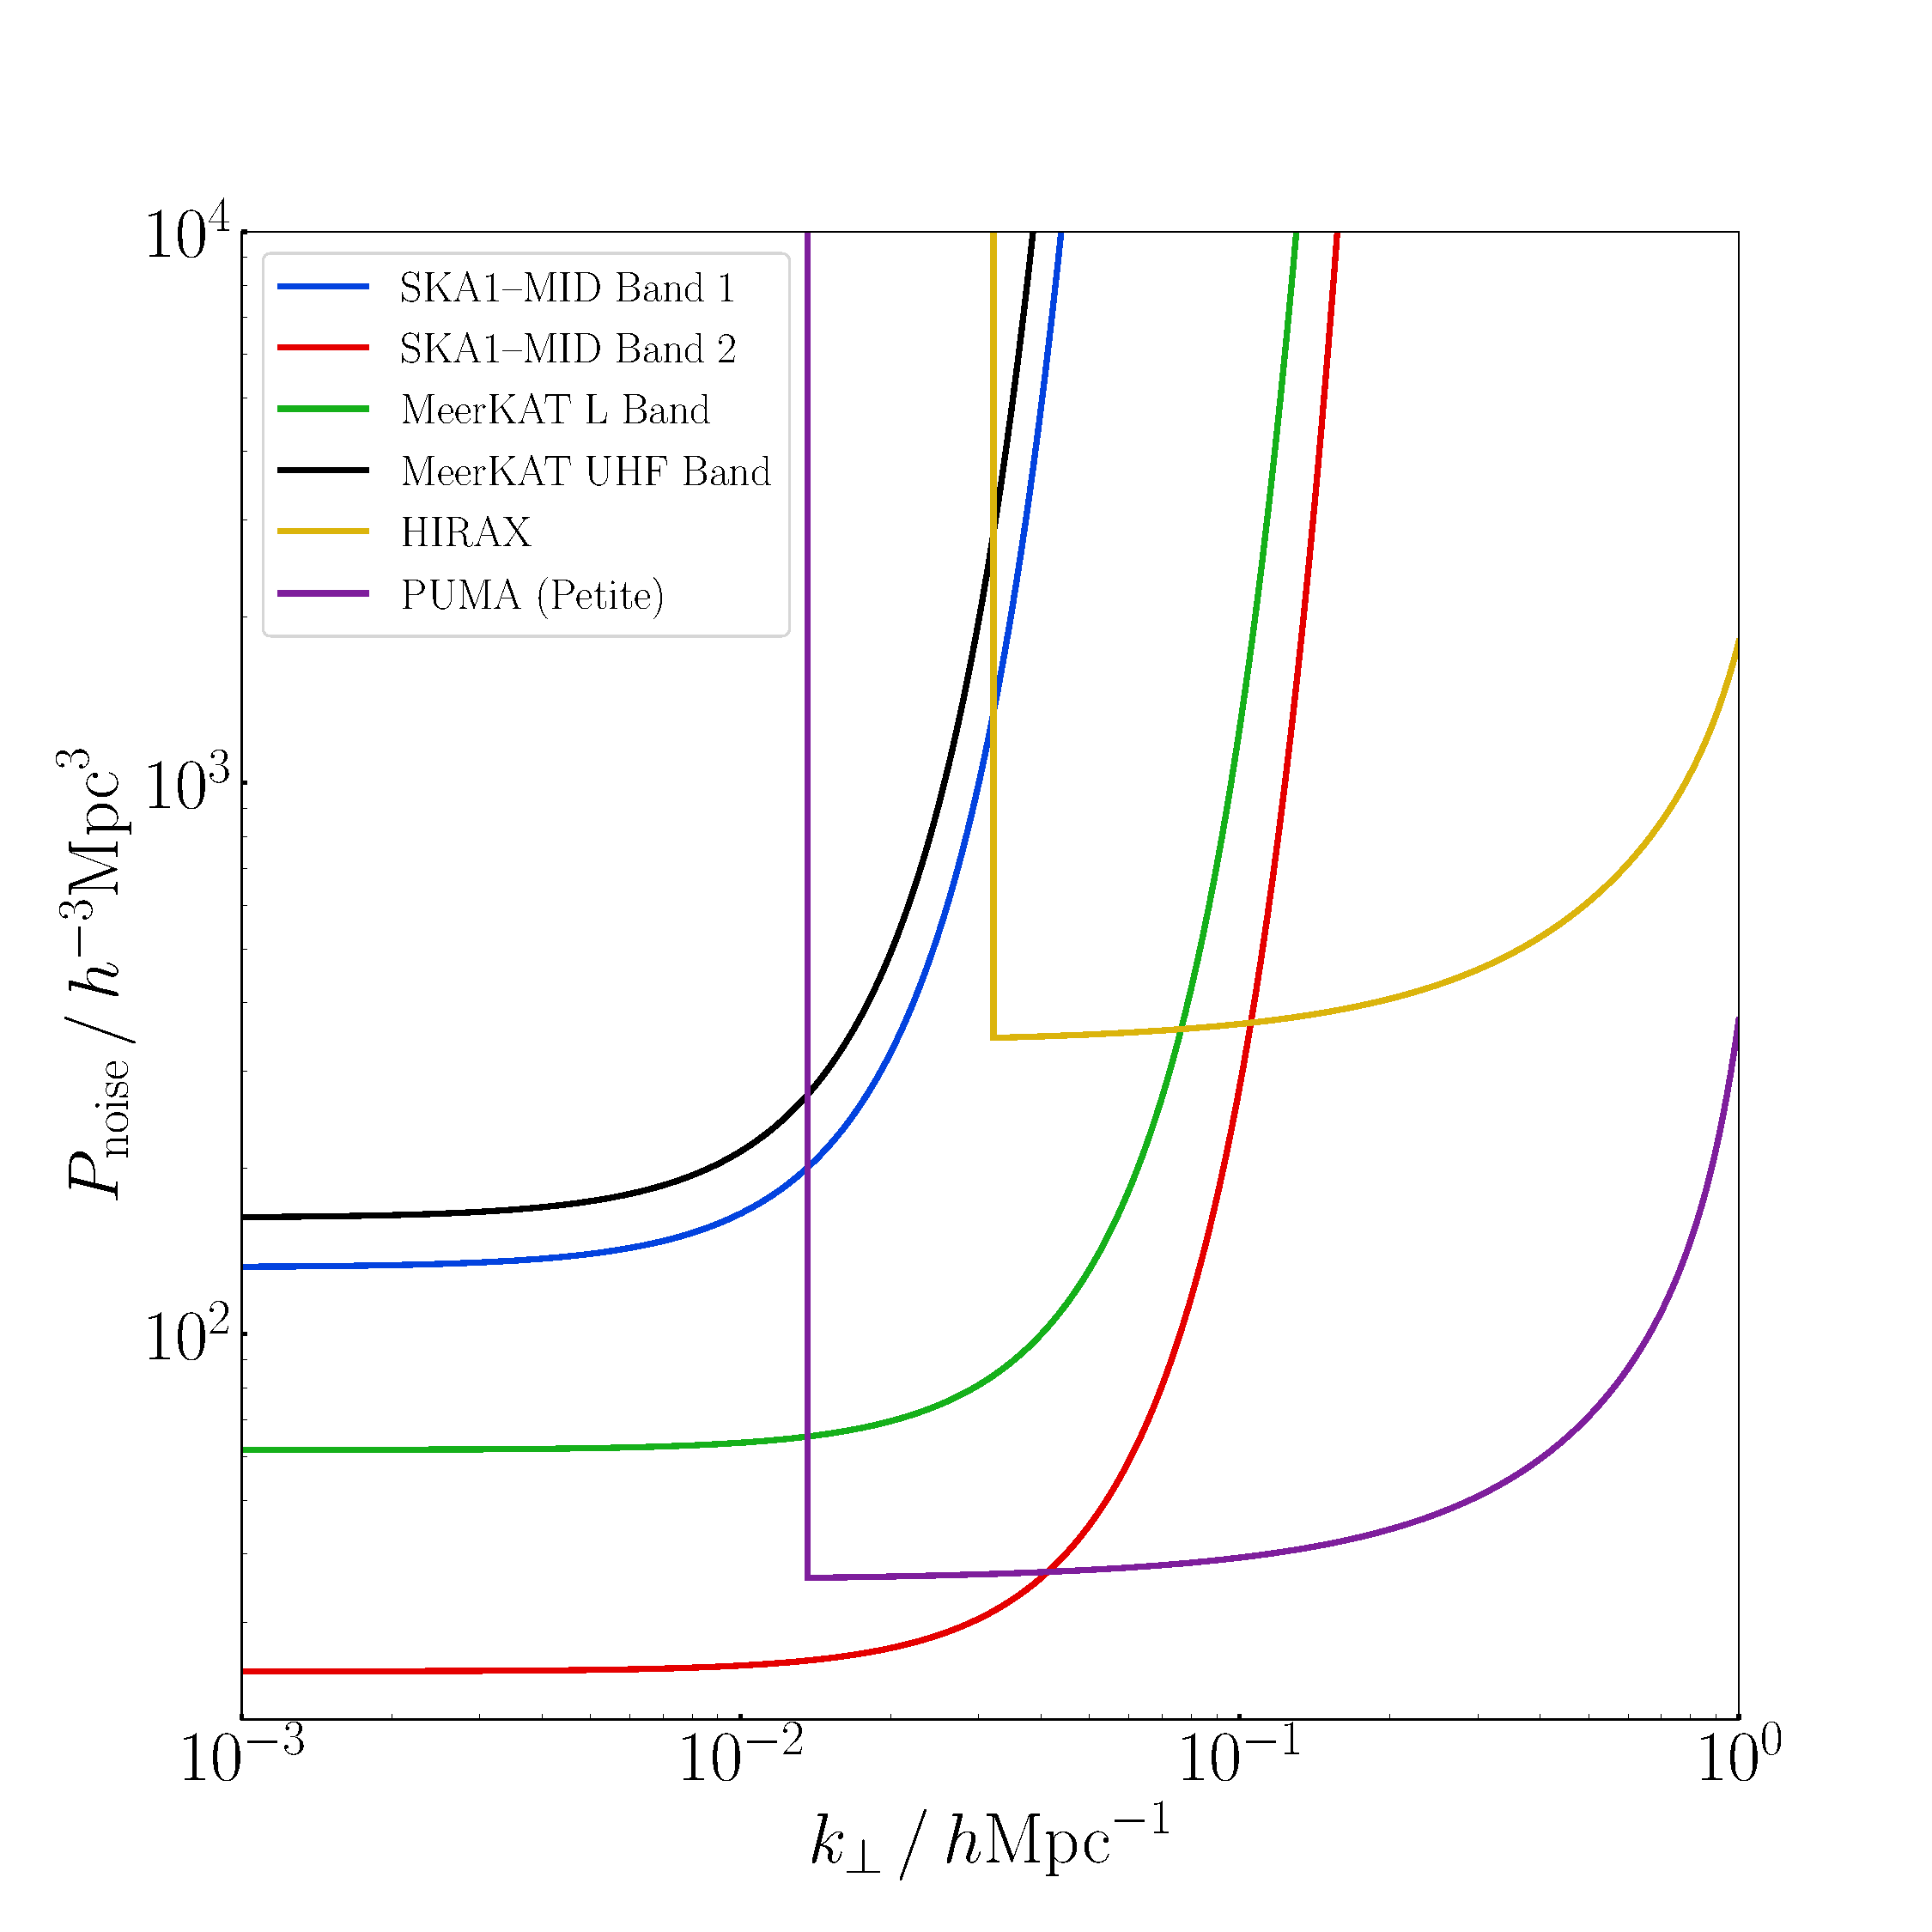
\includegraphics[width=.49\textwidth]{fig/Pnoise}
\vspace*{-0.5cm}
\caption{{Noise power spectra of the SD-mode surveys (at $z=0.4$ for low-$z_\mathrm{max}$ bands and $z=1$ for high-$z_\mathrm{max}$ bands) and IF-mode surveys (HIRAX at $z=1$, PUMA at $z=2$).}}\label{pnoise}
\end{figure}

{In the case of PUMA, we take account of the 50\% fill factor as follows. We use double the number of dishes to define $N_\mathrm{s}$ for the computation of \eqref{e3.4}, i.e. $N_\mathrm{s}^2= 2\times 5000$. Then  we  remove half of the dishes without changing the baseline, i.e. without changing the shape and ground-area of the array.

The noise power spectra of the surveys at fixed redshift are displayed in Figure \ref{pnoise}. For SD-mode surveys, the poor angular resolution is reflected in the blow-up of noise due to the beam in \eqref{sdn}.
The minimum transverse scale for IF-mode surveys  is shown as a sharp cut-off, as in  \eqref{kifmin}, with effectively infinite noise.
 Figure \ref{pnoise} also shows the smooth blow-up of IF-mode noise on small transverse scales, which results  from the fact that 
$n_\mathrm{b}\to 0$ as the baseline approaches its maximum $D_\mathrm{max}$ (see Figure \ref{nbphys}). The unbounded increase of noise kills the signal, corresponding to the approximate cut-off scale \eqref{kifmax}.}


























%
\chapter{Multipoles of the Bispectrum}
\label{chapter:multipoles}

introduction to the full theory : sheeans papers

Above the equality scale the galaxy bispectrum will be  a key probe for measuring primordial non-Gaussianity which can help differentiate between different inflationary models and other theories of the early universe. On these scales a variety of relativistic effects come into play once the galaxy number-count fluctuation is projected onto our past lightcone. By decomposing the Fourier-space bispectrum into invariant multipoles about the observer's line of sight we examine in detail how the relativistic effects contribute to these. We show how to perform this decomposition analytically, which is significantly faster for subsequent computations.  While all multipoles receive a contribution from the relativistic part, odd multipoles arising from the imaginary part of the bispectrum have no Newtonian contribution, making the odd multipoles a smoking gun for a relativistic signature in the bispectrum for single tracers.  The dipole and the octopole are significant on equality scales and above where the Newtonian approximation breaks down. This breakdown is further signified by the fact that the even multipoles receive a significant correction on very large scales.

\section{Introduction}
The bispectrum will play a key role in future galaxy surveys as an  important probe of large-scale structure and for measuring primordial 
non-Gaussianity and galaxy bias~\cite{Jeong:2009vd,Baldauf:2010vn,Celoria:2018euj}. It can help discriminate between different inflationary models and other theories of the early universe, and contains information that is complementary and additional to what is contained in the power spectrum. 
On super-equality scales, a variety of relativistic effects come into play once the galaxy number-count fluctuation is projected onto the past light cone. In the density contrast up to second order, relativistic effects arise from observing on the past lightcone, and they include all redshift, volume and lensing distortions and couplings between these. In Poisson gauge, these effects can be attributed to velocities (Doppler), gravitational potentials (Sachs-Wolfe, integrated SW, time delay) and lensing magnification and shear. In addition, there are corrections arising from a GR definition of galaxy bias~\cite{Bertacca:2014wga}. These effects generate corrections to the Newtonian approximation at order $\mathcal{O}(\cH/k)$ and higher. Non-Gaussianity generated by these relativistic projection effects could closely mimic the signature of \(\fnl\) on large scales which gives a correction in the halo bias $\mathcal{O}((\cH/k)^2)$, indicating the importance of precisely including all $\mathcal{O}(\cH/k)$ and higher effects in theoretical modelling. So far, a variety of relativistic effects in the galaxy Fourier bispectrum has been taken into account, see 
\cite{Umeh:2016nuh,Jolicoeur:2017nyt,Jolicoeur:2017eyi,Jolicoeur:2018blf,Clarkson:2018dwn,Maartens:2019yhx} under the assumption of the plane parallel approximation, and neglecting integrated effects. Other groups are working on this from different angles and approaches, for example by a spherical-Fourier formalism~\cite{Bertacca:2017dzm}, and calculating the angular galaxy bispectrum~\cite{DiDio:2016gpd,DiDio:2018unb}. Crucially, we have shown that the relativistic part should be detectable in a survey like Euclid without resorting to the multi-tracer technique, which is needed for the power spectrum~\cite{Maartens:2019yhx} . 

Once an observable like the galaxy number-count fluctuation is projected onto the past lightcone the orientation of the triangle in the Fourier space bispectrum becomes important. 
Analogously to how the Legendre multipole expansion is used for power spectrum analysis, one can expand the galaxy bispectrum in spherical harmonics, thus isolating the different invariant multipoles with respect to the observer's line of sight $\bm n$. We use the full spherical harmonics for the bispectrum rather than the Legendre polynomial expansion usually adopted for the power spectrum because of the azimuthal degrees of freedom associated with the orientation of the triangle with respect to the line of sight direction vector in Fourier space. In the power spectrum limit, there is only one angular degree of freedom after ensemble averaging. For the bispectrum, we have one angular and one azimuthal degree of freedom which when expanded in spherical harmonics leads to $(2\ell + 1)$ independent harmonics for each multipole value $\ell$. 

This has been done for the Newtonian bispectrum, which generates non-zero multipoles only for even 
\(\ell\) (up to \(\ell = 8\)) due to redshift-space distortions~\cite{Scoccimarro:1999ed,Nan:2017oaq}. Contrary to the Newtonian bispectrum, the relativistic galaxy bispectrum generates non-zero multipoles for both even and odd \(\ell\) up to \(\ell = 8\) and \(m = 6\) where the odd multipoles are induced by the general relativistic effects only. This means that these multipoles are a crucial signature of relativistic projection effects. We provide, for the first time, a multipole decomposition of the Fourier space galaxy bispectrum with relativistic effects included. Additionally we show that the coefficients of this expansion can be worked out analytically. We provide an exact analytic formula for this multipole expansion of the galaxy bispectrum. Previously, we examined for the first time the dipole of the galaxy bispectrum in detail, showing that its amplitude can be more than 10\% of that of the monopole even at equality scales~\cite{Clarkson:2018dwn}. 
In order to eliminate possible biases when analysing large scale structure data, it is important to include the relativistic effects. In addition to this, a variety of the effects that appear in the bispectrum are relativistic effects that have not been measured elsewhere and hence are interesting to study. By analysing the non-zero multipoles of the galaxy bispectrum both for a Euclid-like galaxy survey, and for an SKA-like HI intensity mapping survey, we show the behaviour of the higher multipoles and their corrections to the Newtonian bispectrum. In follow-up work, we are investigating possibilities of detecting the higher multipoles of the bispectrum. See for example~\cite{Maartens:2019yhx} for detection prospects of the leading order relativistic effects; the dipole is expected to have the strongest GR signature. 

The paper is organised as follows. We introduce the relativistic Fourier space bispectrum in section~\ref{sec:relbisp}, and present the multipole expansion of the relativistic bispectrum in section~\ref{sec:extrmulti}. An analysis of the multipoles can be found in section~\ref{sec:anal}. Finally, we summarise our conclusions in section~\ref{sec:concl}.

\section{The relativistic bispectrum}\label{sec:relbisp}

In Fourier space, the observed galaxy bispectrum \(B_g\) at a fixed redshift \(z\) is given by~\cite{Jolicoeur:2017nyt,Jolicoeur:2017eyi}
\begin{equation}
	\langle \Delta_g(z,\ka) \Delta_g(z,\kb) \Delta_g(z,\kc) \rangle = (2\pi)^3 B_g(z,\ka,\kb,\kc) \delta^D(\ka+\kb+\kc),
\end{equation}
where \(\Delta_g(z, \ka)\) is the number count contrast at redshift \(z\) (see~\cite{Jolicoeur:2017nyt} for the full expression). Here we work in the Poisson gauge; note that \(\Delta_g = \delta_g + \text{RSD}+\text{GR}\) projection effects, where the RSD term is the Kaiser RSD up to second order, which is part of the Newtonian approximation. Since redshift is fixed, in what follows we drop redshift dependence for brevity. Furthermore, since the observed direction \(\n\) is fixed in what follows, the plane-parallel approximation is necessarily assumed. Then, at tree level, and for Gaussian initial conditions, the following combinations of terms contribute, 
\begin{equation}
\langle \Delta_g(\ka)\Delta_g(\kb)\Delta_g(\kc) \rangle = \frac{1}{2} \langle \Delta_g^{(1)}(\ka)\Delta_g^{(1)}(\kb)\Delta_g^{(2)}(\kc)\rangle \text{ + 2 cyclic permutations.}
\end{equation}
Using Wick's theorem, this gives an expression for the galaxy bispectrum ~\cite{Jolicoeur:2017nyt}
\begin{equation}
B_g(\ka, \kb,\kc)= \ko^{(1)}(\ka) \ko^{(1)}(\kb) \ko^{(2)}(\ka,\kb,\kc)P(\ka) P(\kb)\text{ + 2 cyclic permutations},
\end{equation}
where \(P\) is the power spectrum of \(\delta_\mathrm{T}^{(1)}\), the first order dark matter density contrast in the total-matter gauge, which corresponds to an Eulerian frame. The first order kernel can be split into a Newtonian and a relativistic part as~\cite{Jeong:2011as}
\begin{equation}
\ko^{(1)} = \ko^{(1)}_\mathrm{N} + \ko^{(1)}_\mathrm{GR}, \qquad \ko^{(1)}_\mathrm{N}= b_1 + f \mu^2, \qquad \ko^{(1)}_\mathrm{GR} = \i \mu \frac{\gamma_1}{k} + \frac{\gamma_2}{k^2}, 
\end{equation}
with \(\mu = \hat\k \cdot \n \) (\(\hat\k = \k/k\)), \(b_1\) is the first-order Eulerian galaxy bias coefficient, \(f\) is the linear growth rate of matter perturbations, and redshift-dependent coefficients \(\gamma_i\) are~\cite{Jeong:2011as},
\begin{align}\label{eq:gamma1def}
\frac{\gamma_1}{\cH} &= f \left[ b_e - 2 \Q - \frac{2(1-\Q)}{\chi \cH} - \frac{\cH'}{\cH^2}\right], \\
\frac{\gamma_2}{\cH^2} &= f(3-b_e) + \frac{3}{2} \Omega_m \left[ 2+ b_e - f - 4\Q - \frac{2(1-\Q)}{\chi\cH} - \frac{\cH'}{\cH^2} \right].\label{eq:gamma2def}
\end{align}
In equations~\eqref{eq:gamma1def}~and~\eqref{eq:gamma2def}, \(\cH\) is the conformal Hubble rate \((\ln a)'\), where a prime denotes a derivative with respect to conformal time; \(b_e\) and \(\Q\) are the galaxy evolution and magnification biases respectively, \(\chi\) is the line-of-sight comoving distance and \(\Omega_m = \Omega_{m0} (1+z) H_0^2/\cH^2\) is the matter density parameter. At first order, the gauge-independent GR definition of galaxy bias is made in the common comoving frame of galaxies and matter, 
\begin{equation}\label{eq:comovinggalaxybiasdef}
	\delta_{g\mathrm{C}}^{(1)} = b_1 \delta_\mathrm{C}^{(1)} =  b_1 \delta_\mathrm{T}^{(1)}\,,
\end{equation}
where subscript C is for the comoving gauge and T is for total matter gauge, which is a gauge corresponding to standard Newtonian perturbation theory. The bias relation in Poisson gauge is then obtained by transforming~\eqref{eq:comovinggalaxybiasdef} to Poisson gauge~\cite{Bertacca:2014wga,Jolicoeur:2017eyi}:
\begin{equation}\label{eq:deltareln}
	\delta_g^{(1)} = \delta_{g\mathrm{C}}^{(1)} + (3 - b_e)\cH v^{(1)} = b_1 \delta_\mathrm{T}^{(1)} + (3-b_e)\cH v^{(1)},
\end{equation}
where \(v^{(1)}\) is the velocity potential. Since \(v^{(1)} =f \cH \delta_T^{(1)}/k^2\), the last term on the right of equation~\eqref{eq:deltareln} leads to the \(f(3-b_e)\) term in \(\gamma_2/\cH^2\), equation~\eqref{eq:gamma2def}.


Similarly to the first order kernel, the second order kernel can be split into a Newtonian and a relativistic part. The second order part of the Newtonian kernel is well studied and is given as~\cite{Bernardeau:2001qr,Karagiannis:2018jdt,Scoccimarro:1999ed,Verde:1998zr}
\begin{align}\label{newt2o}
	\ko_\mathrm{N}^{(2)}(\ka, \kb, \kc) &= b_1 F_2(\ka,\kb) + b_2 + f \mu_3^2 G_2(\ka,\kb) + f Z_2(\ka,\kb) + b_{s^2} S_2(\ka,\kb),
\end{align}
where \(\mu_i = \hat\k_i \cdot \n \), \( b_2\) is the second-order Eulerian bias parameter, and \(b_{s^2} \) is the tidal bias. \(F_2\) and \(G_2\) are the Fourier-space Eulerian kernels for second-order density contrast and velocity respectively~\cite{Jolicoeur:2017nyt,Villa:2015ppa}; 
\begin{align}
F_2(\ka,\kb) &= 1 + \frac{F}{D^2} + \left(\hat{\k}_1 \cdot \hat{\k}_2 \right)\left( \frac{k_1}{k_2} + \frac{k_2}{k_1}\right) + \left( 1-\frac{F}{D^2}\right) \left(\hat{\k}_1 \cdot \hat{\k}_2 \right)^2,\nonumber \\
G_2(\ka,\kb) &= \frac{F'}{D D'} + \left(\hat{\k}_1 \cdot \hat{\k}_2\right)\left(\frac{k_1}{k_2} + \frac{k_2}{k_1} \right) + \left( 2 - \frac{F'}{D D'} \right) \left(\hat{\k}_1 \cdot \hat{\k}_2\right)^2,
\end{align}
where \(F\) is a second-order growth factor, which is given by the growing mode solution of,
\begin{equation}
F'' + \cH F' - \frac{3}{2}\frac{H_0^2 \Omega_{m0}}{a} F = \frac{3}{2}\frac{H_0^2 \Omega_{m0}}{a} D^2.
\end{equation}
 In an Einstein-de Sitter background, \(F= 3 D^2 / 7\), which is a very good approximation for \(\Lambda\)CDM which we use here. The second-order RSD part of the Newtonian kernel is comprised of \(G_2\) above and the kernel \(Z_2\)~\cite{Verde:1998zr,Scoccimarro:1999ed},
\begin{equation}
	Z_2(\ka,\kb) = f \frac{\mu_1 \mu_2}{k_1 k_2}\left( \mu_1 k_1 + \mu_2 k_2 \right)^2 + \frac{b_1 }{k_1 k_2} \left[ \left( \mu_1^2 + \mu_2^2 \right)k_1 k_2 + \mu_1 \mu_2 \left( k_1^2 + k_2^2 \right) \right]\,.
\end{equation}

 Finally, \(S_2(\ka,\kb)\) is the kernel for the tidal bias,
\begin{equation}
	S_2(\ka,\kb) = (\hat{\k}_1 \cdot \hat{\k}_2)^2 - \frac{1}{3}\,.
\end{equation}
The Newtonian bias model is 
\begin{equation}\label{eq:newtbiasmodel}
	\delta_{g\mathrm{T}}^{(2)} = b_1 \delta_\mathrm{T}^{(2)} + b_2 \left[\delta_\mathrm{T}^{(1)}\right]^2 + b_{s^2} s^2\,,
\end{equation}
where \( s^2 = s_{ij}s^{ij}\), and \( s_{ij} = \Phi_{,ij} - \delta_{ij}\nabla^2 \Phi /3\) . 

The relativistic part of the second order kernel was first derived in~\cite{Umeh:2016nuh} in the simplest case and extended in~\cite{Jolicoeur:2017nyt,Jolicoeur:2017eyi,Jolicoeur:2018blf}. Neglecting sub-dominant vector and tensor contributions, we have 
\begin{align}\label{eq:soGRkernel}
\ko_\mathrm{GR}^{(2)}(\ka,\kb,\kc) &= \frac{1}{k_1^2 k_2^2} \left\{ \vphantom{\frac{k_1^2 k_2^2}{k_3}} \beta_1 + E_2(\ka,\kb,\kc) \beta_2 
+\i (\mu_1k_1+\mu_2k_2)\beta_3
+ \i \mu_3 k_3\left[ \beta_{4} + E_2(\ka, \kb, \kc)\beta_{5}\right] \right. \nonumber \\
&\left. +\frac{k_1^2 k_2^2}{k_3^2} \left[ F_2(\ka,\kb) \beta_{6} + G_2(\ka,\kb) \beta_{7} \right] + \left( \mu_1 k_1 \mu_2 k_2 \right)\beta_{8} + \mu_3^2 k_3^2 \left(\beta_{9} + E_2(\ka,\kb,\kc) \beta_{10} \right) \right. \nonumber \\
&\left. + \left(\ka \cdot \kb \right)\beta_{11} + \left( k_1^2 + k_2^2 \right) \beta_{12} + \left( \mu_1^2 k_1^2 + \mu_2^2 k_2^2 \right) \beta_{13} \right. \nonumber \\
&\left. + \i \left[\vphantom{\frac{k_1^2 k_2^2}{k_3}} \left( \mu_1 k_1^3 + \mu_2 k_2^3 \right)\beta_{14} + \left( \mu_1 k_1 + \mu_2 k_2 \right) \left(\ka\cdot\kb \right) \beta_{15} + k_1 k_2 \left(\mu_1 k_2 + \mu_2 k_1 \right) \beta_{16} \right. \right. \nonumber \\
&\left. \left. + \left( \mu_1^3 k_1^3 + \mu_2^3 k_2^3 \right)\beta_{17} + \mu_1 \mu_2 k_1 k_2 \left( \mu_1 k_1 + \mu_2 k_2 \right) \beta_{18} + \mu_3 \frac{k_1^2 k_2^2}{k_3} G_2(\ka,\kb) \beta_{19} \right] \right\}.
\end{align}
We have collected terms according to the overall powers of $k$ involved.
The \(\beta_i\) here are redshift- and bias-dependent coefficients, given in full in appendix  REF BETA APPENDIX, which updates  expressions in previous papers.
We have defined the kernel \(E_2\) which scales as \(k^0\) (like \(F_2\), \(G_2\), and \(Z_2\) do), 
\begin{equation}
E_2(\ka,\kb,\kc) = \frac{k_1^2 k_2^2}{k_3^4} \left[ 3 + 2 \left( \hat{\k}_1 \cdot\hat{\k}_2 \right) \left( \frac{k_1}{k_2} + \frac{k_2}{k_1} \right) + \left( \hat{\k}_1 \cdot \hat{\k}_2 \right)^2 \right],
\end{equation}
which incorporates some of the relativistic dynamical corrections to the intrinsic second-order terms.

At second order, the GR bias model, which corrects the Newtonian bias model~\eqref{eq:newtbiasmodel} is given by~\cite{Umeh:2019qyd},
\begin{equation}
	\delta_{g\mathrm{T}}^{(2)} = b_1 \delta_\mathrm{T}^{(2)} + b_2 \left[ \delta_\mathrm{T}^{(1)} \right]^2 + b_{s^2} s^2 + \delta_{\mathrm{C,GR}}^{(2)}\,,
\end{equation}
where the last term maintains gauge invariance on ultra-large scales, and is given by (using \( \delta_\mathrm{C}^{(1)} =  \delta_\mathrm{T}^{(1)}\) )
\begin{equation}\label{eq:grcorrdelta}
	\delta_{\mathrm{C,GR}}^{(2)} = 2 \cH^2 (3 \Omega_m + 2 f) \left[ \delta_\mathrm{T}^{(1)} \nabla^{-2} \delta_\mathrm{T}^{(1)} - \frac{1}{4} \partial_i \nabla^{-2} \delta_\mathrm{T}^{(1)} \partial^i \nabla^{-2} \delta_\mathrm{T}^{(1)} \right]\,.
\end{equation}
The GR correction~\eqref{eq:grcorrdelta} to the Newtonian bias model is contained in the GR kernel~\eqref{eq:soGRkernel}. Then, we also need to transform \(\delta_{g\mathrm{T}}^{(2)}\) to the Poisson	 gauge \( \delta_g^{(2)} \), the expression for this is given in~\cite{Jolicoeur:2017nyt}, 
\begin{align}
\delta_{g}^{(2)}  &= \delta_{g{\mathrm{T}} }^{(2)} + (3-b_e) \cH v^{(2)} +\Big[ (b_e-3) \cH' + b_e' \cH + (b_e-3)^2 \cH^2 \Big]  \big[v^{(1)}\big]^2 + (b_e-3)\cH   v^{(1)}  v^{(1)\prime} \nonumber\\
& +2(3-b_e)\cH  v^{(1)} \delta_{g{\mathrm{T}}}^{(1)}  - 2  v^{(1)} \delta_{g{\mathrm{T}}}^{(1)\prime} + 3 \left( b_e-3\right) \cH v^{(1)}\Phi^{(1)} \,.\label{dgpt}
\end{align}
All of the terms after $\delta_{g\mathrm{T}}^{(2)}$ on the right of equation~\eqref{dgpt} scale as $(\cH/k)^n \left[ \delta^{(1)}_\mathrm{T} \right]^2$, where $n = 2,4$. Therefore they are omitted in the Newtonian approximation. These GR correction terms maintain gauge-independence on ultra-large scales, and they are included in the GR kernel~\eqref{eq:soGRkernel}.


\section{Extracting the multipoles}\label{sec:extrmulti}

Our goal is to extract the spherical harmonic multipoles of $B_g$ with respect to the observer's line of sight. That is, for a fixed line of sight and triangle shape, the rotation of the plane of the triangle about $\n$ generates invariant moments, the sum of which add up to the full bispectrum. 
 This means that  
\begin{equation}
B_g =\sum_{\ell m} B_{\ell m}Y_{\ell m}(\n)\,,
\end{equation}
where we follow~\cite{Scoccimarro:1999ed,Nan:2017oaq} in our choice of decomposition of the bispectrum (an alternative basis can be found in~\cite{Sugiyama:2018yzo}).
To define the $B_{\ell m}$ we need to define an orientation for the $Y_{\ell m}$ to give the polar and azimuthal angles over which to integrate. We choose a coordinate basis for the vectors that span the triangle as follows: 
\begin{eqnarray}
	&&\k_1 = (0,0,k_1)\, \\
	&&\k_2 = (0, k_2 \sin\theta, k_2 \cos\theta)\,, \\
	&&\k_3 = (0, - k_2 \sin\theta, - k_1 - k_2\cos\theta )\,,\\
	&&\bm{n} = (\sin\theta_1 \cos\varphi, \sin\theta_1 \sin\varphi,\cos\theta_1)\,.
\end{eqnarray}
That is, we fix $\k_1$ along the $z$-axis, and require the other triangle vectors to lie in the $y$-$z$ plane, see figure~\ref{fig:geometry_overview} for a sketch of the relevant vectors. Then we define {\(\mu_1=\cos\theta_1\)} and use $\varphi$, which is the azimuthal angle giving the orientation of the triangle relative to $\n$. \(\theta_{12} = \theta\) is the angle between vectors \(\k_1\) and \(\k_2\), and we define $\mu=\cos\theta=\hat{\k}_1\cdot\hat{\k}_2$.
\begin{figure}[ht]
	\centering
	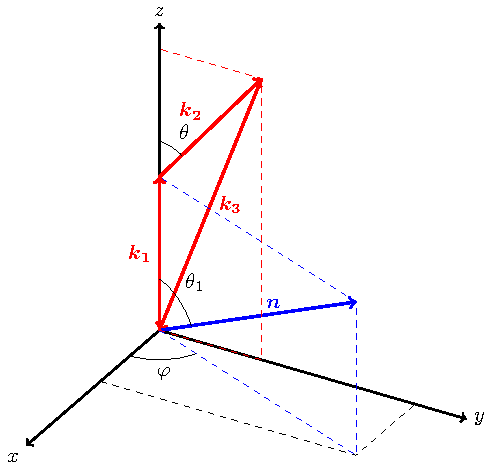
\includegraphics[width=0.6
	\linewidth]{fig/fig.pdf}
	\caption{Overview of the relevant vectors and angles for the Fourier-space bispectrum. \label{fig:geometry_overview} }
\end{figure}

The bispectrum can then be expressed in terms of five variables, \(\varphi\), \(\mu_1\), \(\theta\), \(k_1\) and \(k_2\), by using
\begin{align}
	\mu_2 &= \sqrt{1-\mu_1^2} \sin\theta \sin\varphi + \mu_1\cos\theta\,,  \\
	\mu_3 &= -\frac{k_1}{k_3}\mu_1 - \frac{k_2}{k_3}\mu_2.
\end{align}
Then 
\begin{equation}\label{eq:bgexpv1}
	B_g(\theta, k_1, k_2, \mu_1, \varphi) = \sum_{\ell m} B_{\ell m}(\theta, k_1, k_2) Y_{\ell m} (\mu_1, \varphi)\,,
\end{equation}
where we use standard orthonormal spherical harmonics,
\begin{equation}
	Y_{\ell m}(\mu_1,\varphi) = \sqrt{\frac{2\ell+1}{4 \pi}} \sqrt{\frac{(\ell-m)!}{(\ell+m)!}} P_\ell^m(\mu_1) e^{{\i} m \varphi},
\end{equation}
where the \(P_\ell ^m\) are the associated Legendre polynomials, 
\begin{equation}
	P_\ell ^m(\mu_1) = \frac{(-1)^m}{2^\ell \,\ell !} (1-\mu_1^2)^{m/2} \frac{{\diff}^{\ell +m}}{{\diff}\mu_1^{\ell +m}}(\mu_1^2 - 1)^\ell . 
\end{equation}
At this stage we can extract the multipoles numerically once a bias model and cosmological parameters are given. It is actually significantly quicker to perform this extraction algebraically however, as we now explain. 

The bispectrum in general can be considered as a function of
$k_1,k_2,k_3,\mu,\mu_1, \mu_2, \mu_3$ and $\varphi$. An alternative to the expansion~\eqref{eq:bgexpv1} is 
\begin{equation}\label{eq:bg_absum_reln}
B_g (\mu,k_1,k_2;\mu_1,\mu_2)= \sum_{a=0}^6\sum_{b=0}^6 \mathcal{B}_{ab}(\mu, k_1, k_2)  (\i\mu_1)^a(\i\mu_2)^b\,,
\end{equation}
where we used $\mu_2$ instead of $\varphi$ and $a,b=0\ldots6$, which is the maximum power of $\mu_1,\,\mu_2$ that can arise. This factors out all the angular dependence from the functions $\mathcal{B}_{ab}(\mu,k_1,k_2)$, where $\mu=\cos\theta$, which just depend on the triangle shape (and the cosmology). Note that by explicitly including factors of $\i$ in the sum, we have only real coefficients $\mathcal{B}_{ab}$. 
Schematically we can visualise $\mathcal{B}_{ab}$ in matrix form, split into Newtonian and relativistic contributions as (a bullet denotes a non-zero entry, open circles denote zero entries, and dots are non-existent entries; here that means $a+b > 8$ as higher powers don't occur):
\begin{equation} \label{eq:bab_newtrelmatrix}
\mathcal{B}_{ab}\sim  \underbrace{ 	
\left( 
\begin {array}{ccccccc}  
\bullet& \circ &\bullet& \circ &\bullet& \circ & \circ \\  
\circ  &\bullet& \circ  &\bullet& \circ &\bullet& \circ \\  
\bullet& \circ &\bullet& \circ &\bullet&  \circ&\bullet\\  
\circ  &\bullet& \circ &\bullet& \circ &\bullet& \cdot \\  
\bullet& \circ &\bullet& \circ &\bullet& \cdot &  \cdot\\  
\circ  &\bullet& \circ &\bullet&  \cdot & \cdot & \cdot \\  
\circ  & \circ &\bullet& \cdot & \cdot & \cdot &  \cdot 
\end {array} 
\right)
%\begin{blockarray}{rccccccc}
%a=&~0~&~1~&~2~&~3~&~4~&~5~&~6~\\
%\begin{block}{r(ccccccc)}
%b=0~~&\bullet& \circ &\bullet& \circ &\bullet& \circ & \circ \\  
%1~~&\circ  &\bullet& \circ  &\bullet& \circ &\bullet& \circ \\  
%2~~&\bullet& \circ &\bullet& \circ &\bullet&  \circ&\bullet\\  
%3~~&\circ  &\bullet& \circ &\bullet& \circ &\bullet& \cdot \\  
%4~~&\bullet& \circ &\bullet& \circ &\bullet& \cdot &  \cdot\\  
%5~~&\circ  &\bullet& \circ &\bullet&  \cdot & \cdot & \cdot \\  
%6~~&\circ  & \circ &\bullet& \cdot & \cdot & \cdot &  \cdot \\
%\end{block}
%\end{blockarray}
}_\text{Newtonian}
+
\underbrace{\left( \begin {array}{ccccccc}   \bullet & \bullet & \bullet & \bullet & \bullet & \bullet & \bullet \\   \bullet & \bullet & \bullet & \bullet & \bullet & \bullet & \bullet \\   \bullet & \bullet & \bullet & \bullet & \bullet & \bullet & \circ  \\   \bullet & \bullet & \bullet & \bullet & \bullet & \circ  & \cdot  \\   \bullet & \bullet & \bullet & \bullet & \circ  & \cdot  & \cdot  \\   \bullet &
 \bullet & \bullet &\circ   & \cdot  & \cdot  & \cdot  \\   \bullet & \bullet & \circ  &\cdot   &  \cdot &  \cdot 
& \cdot  \end {array} \right)}_\text{Relativistic}\,.
\end{equation}
(Note that the matrix row and column labelling start at $a,b=0,0$ for the top left element.) 
Thus, the Newtonian contributions always have $a+b=$\,even\,$\leq8$, contributing only to the real part of $B_g$, while there are relativistic contributions present for all $a+b\leq7$. When $a+b$ is odd, this implies an imaginary component to the full bispectrum.  

In terms of the powers of $\cH/k$ involved, we can visualise the maximum powers that appear in matrix form as follows:
\begin{equation}  \label{eq:maxpowerkmatrix}
\mathcal{B}_{ab}\sim \left( \begin {array}{ccccccc} {k}^{-8}&{k}^{-7}&{k}^{-6}&{k}^{-5}&{k
}^{-4}&{k}^{-3}&{k}^{-2}\\  
{k}^{-7}&{k}^{-6}&{k}^{-5
}&{k}^{-4}&{k}^{-3}&{k}^{-2}&{k}^{-1}\\  
{k}^{-6}&{k}
^{-5}&{k}^{-4}&{k}^{-3}&{k}^{-2}&{k}^{-1}&k^0\\  
{k}^{-
5}&{k}^{-4}&{k}^{-3}&{k}^{-2}&{k}^{-1}&k^0 & \cdot\\  
{k}^{-4
}&{k}^{-3}&{k}^{-2}&{k}^{-1}&k^0 &\cdot &\cdot \\  
{k}^{-3}&{k}^{-
2}&{k}^{-1}&k^0 & \cdot&\cdot &\cdot \\  
{k}^{-2}&{k}^{-1}&k^0 &\cdot & \cdot&\cdot & \cdot
\end {array} \right) \,.
\end{equation}

As in the matrix~\eqref{eq:bab_newtrelmatrix}, the matrix row and column labelling in~\eqref{eq:maxpowerkmatrix} starts at $(a,b) = (0,0)$. We see that higher powers $n$ of $(\cH/k)^n$ appear for lower $a+b$. Newtonian contributions are all $({\cal H}/k)^0$. Each element has only odd powers of $\cH/k$ if $a+b$ is odd, and similarly only even powers if $a+b$ is even.

The advantage of writing the bispectrum in this form is that we can derive analytic formulas for the multipoles. We need to find
\begin{align}
B_{\ell m} &= \int{\diff}\Omega \,\,B_g Y^*_{\ell m} \nonumber \\
&= \sum_{a,b} \mathcal{B}_{ab} X_{\ell m}^{ab} \label{eq:xabexp} \,,
\end{align}
where 
\begin{equation} X_{\ell m}^{ab} = \int_0^{2\pi} \diff\varphi\, \int_{-1}^1 \diff\mu_1\, (\i \mu_1)^a (\i \mu_2)^b \,Y_{\ell m}^*(\mu_1,\varphi).
\end{equation}
To do this we use the identity, derived in appendix REF APPENDIX WITH SUM DERIVATION, for $m \geq 0$,
\begin{align}\label{eq:sumformula} X_{\ell m}^{ab} &= 2^{\ell+m-1}\i^{a+b+m}\sqrt{\frac{\pi(2\ell+1)(\ell-m)!}{(\ell+m)!}}\nonumber\\
&\times
\sum_{p=m}^{\frac{1}{2}(b+m)}\sum_{q=m}^{\ell}
\frac{[1+(-1)^{a+b+q}]\,b!\,\cos^{b+m-2p}\theta\sin^{2p-m}\theta}{4^p(b+m-2p)!(\ell-q)!(p-m)!(q-m)!}
%\frac{[\frac{1}{2}(q+\ell-1)]!}{[\frac{1}{2}(q-\ell-1)]!}
%\frac{[\frac{1}{2}(a+b +q-p-1)]!}{[\frac{1}{2}(a+b+q+1)]!}
\frac{\Gamma[\frac{1}{2}(q+\ell+1)]}{\Gamma[\frac{1}{2}(q-\ell+1)]}
\frac{\Gamma[\frac{1}{2}(a+b +q-2p+1)]}{\Gamma[\frac{1}{2}(a+b+q+3)]}
\end{align}
for $m\leq b$ and zero otherwise. For $m < 0$, the result follows a similar pattern, using the simple relation \(X_{\ell -m}^{ab} = (-1)^{a+b+m} X_{\ell m}^{ax`'b*}\), see appendix REF DERIVATION SUM APPENDIX. 

The resulting expressions for $B_{\ell m}$ are rather massive, in part because the cyclic permutations become mixed together, so we do not present them here. We can visualise these in matrix form split into their Newtonian and relativistic contributions:
\begin{equation} \label{eq:blm_newtrelmatrix}
B_{\ell m}=
 \underbrace{\left( \begin {array}{ccccccccc} \bullet& \cdot  &  \cdot& \cdot  &  \cdot& \cdot  &  \cdot& \cdot  &  \cdot
\\  \circ & \circ  &  \cdot& \cdot  &  \cdot& \cdot  &  \cdot& \cdot  &  \cdot \\ \bullet&\bullet&\bullet& \cdot  &  \cdot& \cdot 
& \cdot  &  \cdot& \cdot \\  \circ & \circ  &  \circ& \circ  &  \cdot& \cdot  &  \cdot& \cdot  & \cdot \\ \bullet&\bullet&\bullet
&\bullet&\bullet& \cdot  &  \cdot& \cdot  & \cdot \\ \circ  & \circ  &  \circ& \circ  &  \circ& \circ  &  \cdot& \cdot  & \cdot 
\\ \bullet&\bullet&\bullet&\bullet&\bullet&\bullet&\bullet& \cdot  &  \cdot  \\ \circ  & \circ  &  \circ& \circ  &  \circ&  
\circ & \circ  &  \circ & \cdot \\ \bullet&\bullet&\bullet&\bullet&\bullet&\bullet&\bullet& \circ & \circ \end {array} \right)}_\text{Newtonian}
+
\underbrace{\left( \begin {array}{ccccccccc} \bullet&  \cdot&\cdot  &  \cdot&\cdot  &  \cdot&\cdot  &  \cdot&  \cdot
\\  \bullet&\bullet&  \cdot&\cdot  &  \cdot&\cdot  &  \cdot&\cdot  &  \cdot
\\  \bullet&\bullet&\bullet&  \cdot&\cdot  &  \cdot&\cdot  &  \cdot&  \cdot
\\  \bullet&\bullet&\bullet&\bullet&  \cdot&\cdot  &  \cdot&\cdot  &  \cdot
\\  \bullet&\bullet&\bullet&\bullet&\bullet&  \cdot&\cdot  &  
\cdot & \cdot \\  \bullet&\bullet&\bullet&\bullet&\bullet& \bullet &  \cdot&\cdot  & \cdot \\  \bullet&\bullet&\bullet&\bullet&
\bullet&\bullet&\bullet&  \cdot&  \cdot \\  \bullet&\bullet& \bullet &\bullet&\bullet&\bullet&\bullet& \circ & \cdot \\  \circ  & \circ 
&  \circ&\circ  &  \circ&\circ  &  \circ&\circ  & \circ \end {array} \right)}_\text{Relativistic}\,.
\end{equation}
Again, the matrix indices start at $(0,0$) in the top left, $(\ell,m) = (0,0)$. In the matrix~\eqref{eq:blm_newtrelmatrix}, consistent with previous matrix visualisations, a closed bullet represents a non-zero entry, while an open circle denotes a vanishing entry. The dots denote the non-existent elements of the matrix, here they are matrix elements where \(m > \ell\) and hence do not exist.
So, the Newtonian bispectrum only induces even multipoles up to and including $\ell=8$, while the relativistic part induces even and odd multipoles up to $\ell=7$ with multipoles higher than $\ell = 8$ vanishing exactly. Both the Newtonian and the relativistic part terminate at $m=\pm6$, because $m\leq b\leq6$, as can  be seen from~\eqref{eq:sumformula}. Note that for $m<0$ the pattern is the same.	
In terms of $({\cal H}/k)$ powers, the highest that appear for each $\ell$ is $({\cal H}/k)^{8-\ell}$, while the leading contribution is $({\cal H}/k)^{0~\text{or}~1}$ if the leading contribution is Newtonian or relativistic. These powers are even (odd) if $\ell$ is even (odd), as explained previously along with the visualisation of the powers $\cH/k$ in equation~\eqref{eq:maxpowerkmatrix}.


\subsection*{Presentation of the matrix $\mathcal{B}_{ab}$}

Here we describe in more detail how to calculate the matrix of coefficients $\mathcal{B}_{ab}$. These are far too large to write down, but most of the complexity comes from the $k_i$ permutations and the fact that they are made irreducible from substituting for $\mu_3$. However, the core part can be shown from which they can easily be calculated. First we note that once $\mu_3$ is substituted for, we can write the first cyclic permutation of the product of the kernels as  
\begin{equation}
	\ko_{123}=\ko^{(1)}(k_1,\mu_1)\ko^{(1)}(k_2,\mu_2)\ko^{(2)}(k_1,k_2,k_3,\mu_1,\mu_2)= \sum_{a=0}^5\sum_{b=0}^5 (\i \mu_1)^a (\i \mu_2)^b \ko_{ab}(k_1,k_2,k_3)\,,
\end{equation}
where \(\ko_{ab}(k_1,k_2,k_3)=\ko_{ab}(k_2,k_1,k_3)\) is a set of real \(\mu\)-independent coefficients which we give below, and here the maximum value of \(a,\,b = 5\). Given $\ko_{123}$ we can derive the permutations $\ko_{321}$ and $\ko_{312}$ as
\begin{align}
	&\ko_{321} = \sum_{a,b} \sum_{c=0}^a \binom{a}{c} \frac{k_1^{a-c} k_2^c}{k_3^a} (-1)^a (\i \mu_1)^{a-c} (\i \mu_2)^{b+c} \ko_{ab}(k_3,k_2,k_1)\label{eq:ko_321perm}, \\
	&\ko_{312} = \sum_{a,b} \sum_{c=0}^a \binom{a}{c} \frac{k_1^{a-c} k_2^c}{k_3^a} (-1)^a (\i \mu_1)^{a+b-c} (\i \mu_2)^{c} \ko_{ab}(k_3,k_1,k_2),\label{eq:ko_312perm}
\end{align} 
where, as in general, the range of \(a,\,b = 0 \dots 6\).
Given these, the full bispectrum is just $B_g=\ko_{123}P_1P_2+2\,$permutations, but now explicitly written in terms of sums over powers of $\mu_1,\mu_2$.  From this $\mathcal{B}_{ab}$ can be found by inspection. The difference in dimension between the permutations originates from the other cyclic permutations being added, where one substitutes \(\mu_3 = - \left( k_1 \mu_1 + k_2 \mu_2 \right)/k_3\). In~\eqref{eq:ko_321perm}  the largest power of $\mu_2$ is 6, and~\eqref{eq:ko_312perm} has the largest power of $\mu_1$ as 6.

To present $\ko_{ab}(k_1,k_2,k_3)$ we will show powers of ${\cal H}/k$ separately, and write $\ko_{ab}(k_1,k_2,k_3)=\sum_{n=0}^8 \ko_{ab}^{(n)}(k_1,k_2,k_3)$ where $n$ represents the power of ${\cal H}/k$.  Then the Newtonian and leading GR correction  part look like (again, a bullet denotes a non-zero entry)
\begin{equation}         
  \ko_{ab}^{(0)} = \left( \begin {array}{cccccc} 
 \bullet&\circ &\bullet&\circ &\bullet&\circ \\ 
  \circ &\bullet&\circ &\bullet &\circ &\bullet\\ 
   \bullet&\circ &\bullet&\circ &\bullet&\circ \\ 
    \circ &\bullet&\circ &\bullet&\circ &\bullet\\ 
 \bullet&\circ &\bullet&\circ &\bullet&\circ \\ 
  \circ &\bullet&\circ &\bullet&\circ &\circ 
\end {array} \right)~~~~~ 
\ko_{ab}^{(1)} = \left( \begin {array}{cccccc} 
  \circ&\bullet&\circ&\bullet&\circ&\bullet\\ \bullet&\circ&\bullet&\circ
&\bullet&\circ\\ \circ&\bullet&\circ&\bullet&\circ&\bullet\\ \bullet&\circ&\bullet&\circ&\bullet&\circ
\\ \circ&\bullet&\circ&\bullet&\circ&\circ\\ \bullet&\circ&\bullet&\circ&\circ&\circ
\end {array}
  \right)
\end{equation}
where, writing $F=F_2(\bm k_1,\bm k_2)$, $G=G_2(\bm k_1,\bm k_2)$, $S=S_2(\bm k_1,\bm k_2)$,  
\begin{align}
\ko^{(0)}_{00}&= 
b_{1}^{2}\left(b_{s^2} S+b_{2}\right)+F b_{1}^{3}
 \\ \ko^{(0)}_{02}&= - b_1f
 \left[b_{1}^{2}+b_{s^2} S +b_{2}+\left(F+\frac{G k_{2}^{2}}{k_{3}^{2}}\right) b_{1}\right]
 \\ \ko^{(0)}_{04}&= 
b_1f^2 \left(\frac{G k_{2}^{2} }{k_{3}^{2}}+b_{1}\right)
 \\ \ko^{(0)}_{11}&= 
-b_1^2f\left[\frac{\left(k_{1}^{2}+k_{2}^{2}\right) b_{1}}{k_{1} k_{2}}+\frac{2 G k_{1}  k_{2} }{k_{3}^{2}}\right] 
 \\ \ko^{(0)}_{13}&= 
 b_1f^2\left[\frac{\left(k_{1}^{2}+2 k_{2}^{2}\right) b_{1}}{k_{1} k_{2}}+\frac{2 G k_{1}  k_{2} }{k_{3}^{2}}\right]
 \\ \ko^{(0)}_{15}&= 
-\frac{b_{1}f^{3} k_{2} }{k_{1}}
 \\ \ko^{(0)}_{20}&= 
- b_1 f \left[b_{1}^{2}+b_{s^2} S + b_{2}+\left(F+\frac{G k_{1}^{2}}{k_{3}^{2}}\right) b_{1}\right]
 \\ \ko^{(0)}_{22}&= 
f^{2}\left[4 b_{1}^{2}+b_{s^2} S+b_{2}+\left(F+\frac{G\left(k_{1}^{2}+k_{2}^{2}\right)}{k_{3}^{2}}\right) b_{1}\right]
 \\ \ko^{(0)}_{24}&= 
 -f^{3}\left(\frac{G k_{2}^{2}}{k_{3}^{2}}+3 b_{1}\right) 
 \\ \ko^{(0)}_{31}&= 
b_1f^{2}\left[\frac{b_{1}\left(2 k_{1}^{2}+k_{2}^{2}\right) }{k_{1} k_{2}}+\frac{2 G k_{1}  k_{2} }{k_{3}^{2}}\right] 
 \\ \ko^{(0)}_{33}&= 
 -f^{3}\left[\frac{2b_{1}\left(k_{1}^{2}+k_{2}^{2}\right) }{k_{1} k_{2}}+\frac{2 G k_{1}  k_{2}}{k_{3}^{2}}\right]
 \\ \ko^{(0)}_{35}&= 
\frac{f^{4} k_{2}}{k_{1}}
 \\ \ko^{(0)}_{40}&= 
b_{1}f^{2}\left(b_1+\frac{G k_{1}^{2} }{k_{3}^{2}}\right) 
 \\ \ko^{(0)}_{42}&= 
 -f^3\left(3b_{{1}}+ {\frac {Gk_{{1}}^{2}}{k_{{3}}^{2}}}
 \right)
 \\ \ko^{(0)}_{44}&= 
2 f^{4}
 \\ \ko^{(0)}_{51}&= 
-\frac{ b_{1}f^{3} k_{1}}{k_{2}}
 \\ \ko^{(0)}_{53}&= 
\frac{f^{4} k_{1}}{k_{2}}.
\end{align}
Similarly, the leading GR correction $\mathcal{O}(\cH/k)$  coefficients are, 
\begin{align}
\ko^{(1)}_{01}=&
 b_{1}\gamma_{1}\frac{\left( b_{2}+b_{s^2} S \right)}{k_{2}}
+ b_{1}^{2}
\left(\frac{F \gamma_{1}+\beta_{16}}{k_{2}}+\frac{\beta_{15} \mu}{k_{1}}+\frac{\beta_{14}k_{2} }{k_{1}^{2}}-\frac{  \beta_{19}G k_{2}}{k_{3}^{2}}\right)
%
 \\ \ko^{(1)}_{03}=& b_{1}f\left[\frac{\left(\beta_{19}-\gamma_{1}\right) G k_{2}}{k_{3}^{2}}-\frac{\beta_{16}}{k_{2}}-\frac{\beta_{15} \mu}{k_{1}}-\frac{\beta_{14} k_{2} }{k_{1}^{2}}\right] 
 -b_{1}^{2}\left(\frac{f \gamma_{1}}{k_{2}}+\frac{ \beta_{17}k_{2}}{k_{1}^{2}}\right) 
 %
 \\ \ko^{(1)}_{05}=&  \frac{b_{1}f \beta_{17}k_{2} }{k_{1}^{2}}
 \\ \ko^{(1)}_{10}=& b_{1}\gamma_{1}\frac{\left(b_{2}+b_{s^2} S \right)}{k_{1}}+  b_{1}^{2}\left[\left(-\frac{G \beta_{19}}{k_{3}^{2}}+\frac{\beta_{14}}{k_{2}^{2}}\right) k_{1}+\frac{\beta_{15} \mu}{k_{2}}+\frac{F \gamma_{1}+\beta_{16}}{k_{1}}\right]
 %
 \\ \ko^{(1)}_{12}=&  - \gamma_{1} f\frac{\left(b_{s^2} S+b_{2}\right)}{k_{1}}-  b_{1}^{2}\left[\gamma_{1} f\left(\frac{k_{1}}{k_{2}^{2}}+\frac{2}{k_{1}}\right) +\frac{\beta_{18}}{k_{1}}\right]\\&
 + b_{1}f\left\{\left[\left(-\frac{2 k_{1}}{k_{3}^{2}}-\frac{k_{2}^{2}}{k_{1} k_{3}^{2}}\right) \gamma_{1}+\frac{k_{1} \beta_{19}}{k_{3}^{2}}\right] G-\frac{F \gamma_{1}}{k_{1}}-\frac{\beta_{14} k_{1}}{k_{2}^{2}}-\frac{\beta_{15} \mu}{k_{2}}-\frac{\beta_{16}}{k_{1}}\right\}
 %%
 \\ \ko^{(1)}_{14}=&  b_{1}f\frac{2 \gamma_{1} f+\beta_{18}}{k_{1}}+\frac{G k_{2}^{2} \gamma_{1} f^{2}}{k_{1} k_{3}^{2}}
 %%
 \\ \ko^{(1)}_{21}=& -\gamma_{1} f\frac{\left(b_{s^2} S+ b_{2}\right)}{k_{2}}
  -b_{1}^{2}\left[\gamma_1 f\left(\frac{2}{k_{2}}+\frac{k_{2}}{k_{1}^{2}}\right) +\frac{\beta_{18}}{k_{2}}\right] \\
 &+b_1f\left\{\left[\left(-\frac{k_{1}^{2}}{k_{2} k_{3}^{2}}-\frac{2 k_{2}}{k_{3}^{2}}\right) \gamma_{1}+\frac{k_{2} \beta_{19}}{k_{3}^{2}}\right] G-\frac{F \gamma_{1}}{k_{2}}-\frac{\beta_{16}}{k_{2}}-\beta_{14}\left(\frac{ \mu}{k_{1}}+\frac{k_{2} }{k_{1}^{2}}\right)\right\}
 %%
 \\ \ko^{(1)}_{23}=&  b_{1}f\left[\left(\frac{4}{k_{2}}+\frac{2 k_{2}}{k_{1}^{2}}\right) \gamma_{1} f+\frac{\beta_{18}}{k_{2}}+\frac{\beta_{17} k_{2} }{k_{1}^{2}} \right]+f^{2}\left[G\left(3 \gamma_{1}-\beta_{19}\right) \frac{k_{2} }{k_{3}^{2}}+\frac{\beta_{16}}{k_{2}}+\frac{\beta_{15} \mu}{k_{1}}+\frac{\beta_{14} k_{2} }{k_{1}^{2}}\right]
 %%
 \\ \ko^{(1)}_{25}=& -f^2(\gamma_1f+\beta_{17})\frac{k_{2} }{k_{1}^{2}}
 %%
 \\ \ko^{(1)}_{30}=& - b_{1}^{2}\left(\frac{f \gamma_{1}}{k_{1}}+\frac{\beta_{17} k_{1} }{k_{2}^{2}}\right)+b_{1}f\left[G\left(- \gamma_{1}+\beta_{19}\right)  \frac{k_{1} }{k_{3}^{2}}-\frac{\beta_{14} k_{1}}{k_{2}^{2}}-\frac{\beta_{15} \mu}{k_{2}}-\frac{\beta_{16}}{k_{1}}\right] 
 %%
 \\ \ko^{(1)}_{32}=& b_{1}f\left[\left(\frac{2 k_{1}}{k_{2}^{2}}+\frac{4}{k_{1}}\right) \gamma_{1} f+\frac{ \beta_{17} k_{1}}{k_{2}^{2}}+\frac{\beta_{18}}{k_{1}}\right] +f^2\left[G\left(3 \gamma_{1}- \beta_{19}\right) \frac{k_{1} }{k_{3}^{2}}+\frac{\beta_{14} k_{1}}{k_{2}^{2}}+\frac{\beta_{15} \mu}{k_{2}}+\frac{\beta_{16}}{k_{1}}\right]
 %%
 \\ \ko^{(1)}_{34}=& -\frac{f^{2}\left(3 f \gamma_{1}+\beta_{18}\right)}{k_{1}}
 % %
 \\ \ko^{(1)}_{41}=& b_{1}f\frac{\left(2 \gamma_{1} f+ \beta_{18}\right)}{k_{2}} +\frac{G \gamma_{1} f^{2} k_{1}^{2} }{k_{2} k_{3}^{2}}
 %%
 \\ \ko^{(1)}_{43}=&-\frac{f^{2}\left(3 f \gamma_{1}+\beta_{18}\right)}{k_{2}}
 %
 \\ \ko^{(1)}_{50}=& \frac{b_1 \beta_{17} f k_1}{k_2^2}
 \\ \ko^{(1)}_{52}=&-\frac{f^{2} k_{1}\left(f \gamma_{1}+\beta_{17}\right)}{k_{2}^{2}}\,.
\end{align}
The remaining matrices are of the form 
\begin{align}
 \ko^{(2)}_{ab}&= 
 \left( \begin {array}{cccccc} \bullet &\circ &\bullet &\circ 
&\bullet &\circ \\  \circ &\bullet &\circ &
\bullet &\circ &\bullet \\  \bullet &\circ 
&\bullet &\circ &\bullet &\circ \\  \circ &
\bullet &\circ &\bullet &\circ &\circ \\  
\bullet &\circ &\bullet &\circ &\circ &\circ 
\\  \circ &\bullet &\circ &\circ &\circ &
\circ \end {array} \right) 
~~~ \ko^{(3)}_{ab}= 
 \left( \begin {array}{cccccc} \circ &\bullet &\circ &\bullet 
&\circ &\bullet \\  \bullet &\circ &
\bullet &\circ &\bullet &\circ \\  \circ &
\bullet &\circ &\bullet &\circ &\circ \\  
\bullet &\circ &\bullet &\circ &\circ &\circ 
\\  \circ &\bullet &\circ &\circ &\circ &
\circ \\  \bullet &\circ &\circ &\circ &
\circ &\circ \end {array} \right) 
~~~ \ko^{(4)}_{ab}= 
 \left( \begin {array}{cccccc} \bullet &\circ &\bullet &\circ 
&\bullet &\circ \\  \circ &\bullet &\circ &
\bullet &\circ &\circ \\  \bullet &\circ &
\bullet &\circ &\circ &\circ \\  \circ &
\bullet &\circ &\circ &\circ &\circ \\  
\bullet &\circ &\circ &\circ &\circ &\circ 
\\  \circ &\circ &\circ &\circ &\circ &
\circ \end {array} \right) 
~~~ \ko^{(5)}_{ab}= 
 \left( \begin {array}{cccccc} \circ &\bullet &\circ &\bullet 
&\circ &\circ \\  \bullet &\circ &\bullet &
\circ &\circ &\circ \\  \circ &\bullet &
\circ &\circ &\circ &\circ \\  \bullet &
\circ &\circ &\circ &\circ &\circ \\  
\circ &\circ &\circ &\circ &\circ &\circ 
\\  \circ &\circ &\circ &\circ &\circ &
\circ \end {array} \right) \nonumber
\\ \ko^{(6)}_{ab}&= 
 \left( \begin {array}{cccccc} \bullet &\circ &\bullet &\circ 
&\circ &\circ \\  \circ &\bullet &\circ &
\circ &\circ &\circ \\  \bullet &\circ &
\circ &\circ &\circ &\circ \\  \circ &
\circ &\circ &\circ &\circ &\circ \\  
\circ &\circ &\circ &\circ &\circ &\circ 
\\  \circ &\circ &\circ &\circ &\circ &
\circ \end {array} \right) 
~~~ \ko^{(7)}_{ab}= 
 \left( \begin {array}{cccccc} \circ &\bullet &\circ &\circ &
\circ &\circ \\  \bullet &\circ &\circ &
\circ &\circ &\circ \\  \circ &\circ &
\circ &\circ &\circ &\circ \\  \circ &
\circ &\circ &\circ &\circ &\circ \\  
\circ &\circ &\circ &\circ &\circ &\circ 
\\  \circ &\circ &\circ &\circ &\circ &
\circ \end {array} \right) 
~~~ \ko^{(8)}_{ab}= 
 \left( \begin {array}{cccccc} \bullet &\circ &\circ &\circ &
\circ &\circ \\  \circ &\circ &\circ &
\circ &\circ &\circ \\  \circ &\circ &
\circ &\circ &\circ &\circ \\  \circ &
\circ &\circ &\circ &\circ &\circ \\  
\circ &\circ &\circ &\circ &\circ &\circ 
\\  \circ &\circ &\circ &\circ &\circ &
\circ \end {array} \right).
\end{align}
Their coefficients are extracted in similar fashion, and can be found in full in appendix  REF APPENDIX Kab COEFF%~\ref{sec:kabappendix}. 



\section{Analysis}\label{sec:anal}

Here we present an analysis of the behaviour of the  multipoles. 

\subsection*{ Co-linear, squeezed and equilateral limits}


To help understand further the multipoles we can evaluate their equilateral $(k_1=k_2=k_3)$, co-linear ($\theta=0$ or $\theta=\pi$) and squeezed limits analytically.  
Non-zero co-linear multipoles exist only for $m=0$ components. This is the one limit that is easy to evaluate by hand~-- it follows directly from~\eqref{eq:sumformula}. 
The equilateral case is significantly more complicated to evaluate.
Non-zero equilateral multipoles exist for all even $m$, for any $\ell$, the one exception being the $m=0$ part of the dipole, for which the equilateral configuration is identically zero. These are summarised in Fig.~\ref{fig:blm_overview}, together with the powers of $k$ which appear in each multipole.
\begin{figure}[ht]
\centering
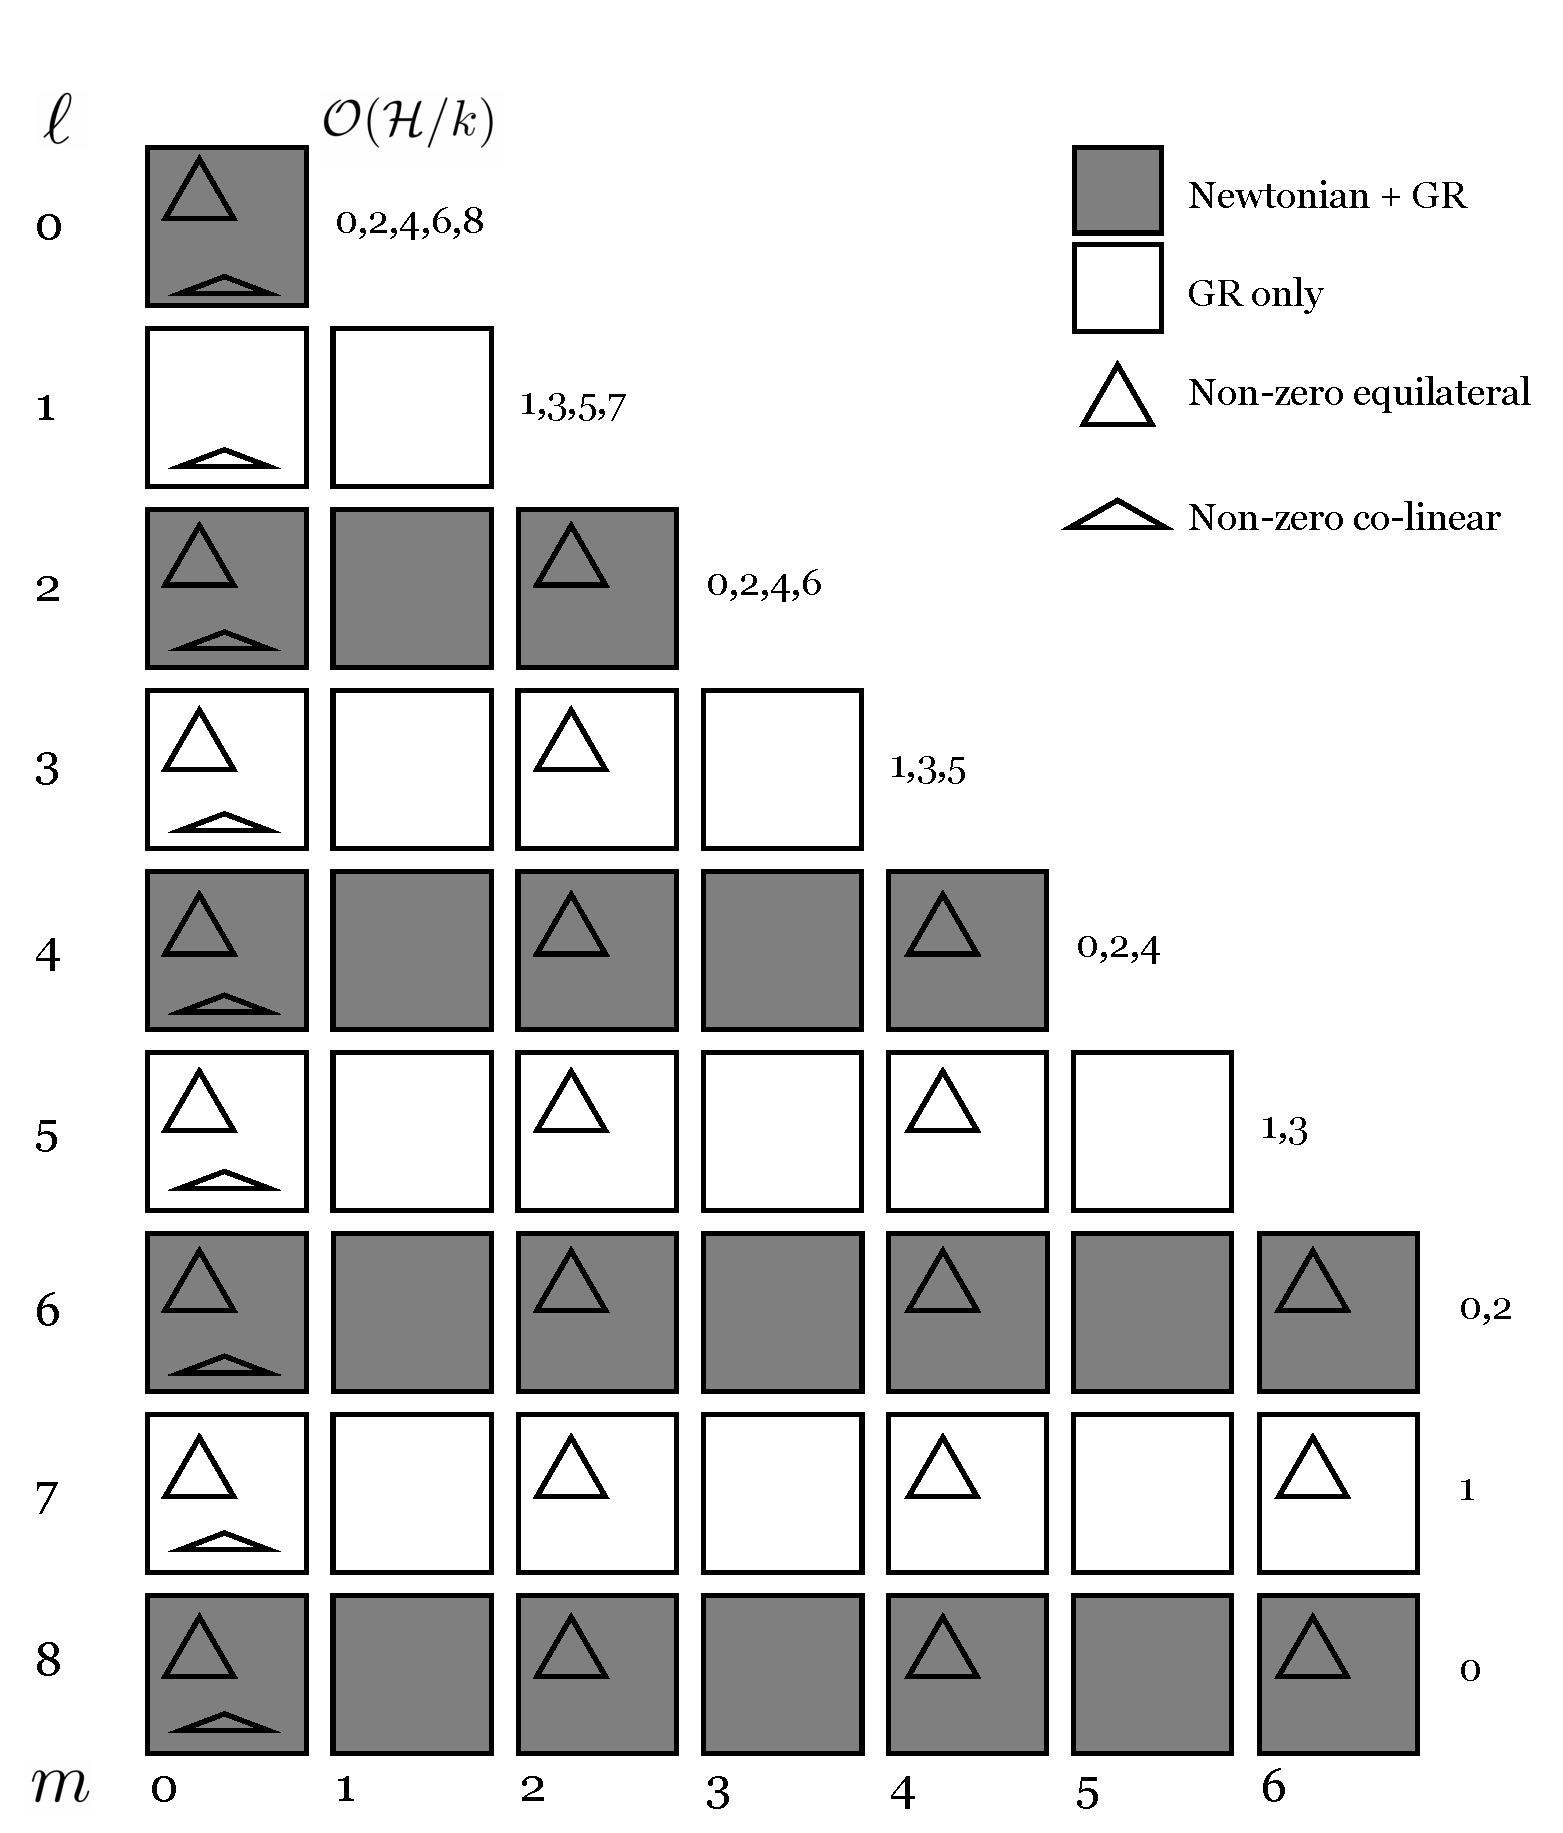
\includegraphics[width=0.5\textwidth]{fig/overview.pdf}
\caption{Overview of all non-zero multipoles for the bispectrum, which includes $\ell$ from 0 to 8, and $m$ from $-\ell$ to $\ell$; the pattern here is the same for $m < 0$, so only $m \geq 0$ are displayed. Denoted in the figure are whether components are Newtonian+GR or GR only, triangle shapes indicating whether given components are non-vanishing in flattened (co-linear) or equilateral limits. Note how the dipole is unique in having the equilateral case vanish for every value of \(m\). Also given is which powers of $\cH/k$ appear in each of the multipoles. \label{fig:blm_overview}}
\end{figure}

The squeezed limit was explicitly evaluated in~\cite{Clarkson:2018dwn} for the leading $\mathcal{O}(\mathcal{H}/k_L)$ contribution, where $k_L$ is the long mode, which we expand further here. {Note that in what follows, we have assumed that the small-scale modes are sufficiently sub-equality scale, and that the large-scale modes are larger than the equality scale. The leading corrections in the even multipoles require us going beyond leading order $\mathcal{O}(\mathcal{H}/k_L)$ in the squeezed limit. We let 
\begin{equation}
k_{1}=k_{2}=k_S, ~~k_{3}=\epsilon k_S\,,
\end{equation}
to write the wavenumber in terms of the short mode $k_S\gg k_L$, which implies
\begin{equation}
\mu=-1+\frac{\epsilon^2}{2}\,.
\end{equation}
We then take the limit as $\epsilon\to0$ with the short mode $k_S$ fixed, and keep only the leading terms in $\cH/k_L$, neglecting factors of $\cH/k_S$ and $P(k_S)^2$.  For each multipole we are then left with the squeezed limit as a polynomial in $\cH/k_L$. The leading contributions are:
\begin{equation}
\underbrace{\left(\frac{\cH}{k_L}\right)^0 
 \left( \begin {array}{ccccccccc} \bullet &\cdot &\cdot &\cdot &\cdot &\cdot &\cdot &\cdot &\cdot 
\\  \circ &\circ &\cdot &\cdot &\cdot &\cdot &\cdot &\cdot &\cdot \\  \bullet &\circ &\bullet &\cdot &\cdot &\cdot 
&\cdot &\cdot &\cdot \\  \circ &\circ &\circ &\circ &\cdot &\cdot &\cdot &\cdot &\cdot \\  \bullet &\circ &\bullet 
&\circ &\bullet &\cdot &\cdot &\cdot &\cdot \\  \circ &\circ &\circ &\circ &\circ &\circ &\cdot &\cdot &\cdot 
\\  \bullet &\circ &\bullet &\circ &\bullet &\circ &\circ &\cdot &\cdot \\  \circ &\circ &\circ &\circ &\circ &\circ 
&\circ &\circ &\cdot \\  \bullet &\circ &\bullet &\circ &\bullet &\circ &\circ &\circ &\circ \end {array} \right) 
}_{\text{Newtonian part}}
+
%%
\underbrace{
 \left(\frac{\cH}{k_L}\right)^1\left( \begin {array}{ccccccccc} {\circ }&\cdot &\cdot &\cdot &\cdot &\cdot &\cdot &\cdot &\cdot \\ \circ &\bullet &\cdot &\cdot &\cdot &\cdot &\cdot &\cdot &\cdot \\ {\circ }&\circ &{\circ }&\cdot &\cdot &\cdot &\cdot &\cdot &\cdot \\ \circ &\bullet &\circ &\bullet &\cdot &\cdot &\cdot &\cdot &\cdot \\ {\circ }&\circ &{\circ }&\circ &\circ &\cdot &\cdot &\cdot &\cdot \\ \circ &\bullet &\circ &\bullet &\circ &\circ &\cdot &\cdot &\cdot \\ {\circ }&\circ &{\circ }&\circ &\circ &\circ &\circ &\cdot &\cdot \\ \circ &\bullet &\circ &\bullet &\circ &\circ &\circ &\circ &\cdot \\ \circ &\circ &\circ &\circ &\circ &\circ &\circ &\circ &\circ \end {array} \right) 
+
%%
\left(\frac{\cH}{k_L}\right)^2 \left( \begin {array}{ccccccccc} \bullet &\cdot &\cdot &\cdot &\cdot &\cdot &\cdot &\cdot &\cdot \\ \circ &\circ &\cdot &\cdot &\cdot &\cdot &\cdot &\cdot &\cdot \\ \bullet &\circ &\bullet &\cdot &\cdot &\cdot &\cdot &\cdot &\cdot \\ \circ &\circ &\circ &\circ &\cdot &\cdot &\cdot &\cdot &\cdot \\ \bullet &\circ &\bullet &\circ &\circ &\cdot &\cdot &\cdot &\cdot \\ \circ &\circ &\circ &\circ &\circ &\circ &\cdot &\cdot &\cdot \\ \bullet &\circ &\bullet &\circ &\circ &\circ &\circ &\cdot &\cdot \\ \circ &\circ &\circ &\circ &\circ &\circ &\circ &\circ &\cdot \\ \circ &\circ &\circ &\circ &\circ &\circ &\circ &\circ &\circ \end {array} \right) }_\text{GR contributions}
\end{equation}
Here, the matrices represent the $\ell,m$ values from $\ell=0,m=0$ (top left entry). We see that the Newtonian part has non-zero squeezed limits for some even $m$, terminating at $m=4$. GR corrections come in up to $m=3$ for $\ell\leq 7$. For odd $m$ these contributions come in for the leading terms $\mathcal{O}(\mathcal{H}/k)$, while for $m$ even the order is lower, $\mathcal{O}((\mathcal{H}/k)^2)$. Note that we assume primordial Gaussianity. In the presence of primordial non-Gaussianity, the squeezed limit has higher powers of $\cH/k$. Current work investigates how primordial non-Gaussianity will change our results. The effect of local primordial non-Gaussianity on the Newtonian galaxy bispectrum is presented in~\cite{Umeh:2016nuh}.


\subsection*{Numerical results}

Here we present a numerical analysis of the multipoles of the galaxy bispectrum. We use three different survey models, two of which are appropriate for future surveys; i.e. SKA HI intensity mapping, and a Stage IV \(H\alpha\) spectroscopic galaxy survey similar to Euclid. The third model we consider is a simplified `toy model' for illustrative purposes. The parameters we use are introduced below. 

Evolution and magnification bias are defined as~\cite{Alonso:2015uua}, 
\begin{equation}\label{eq:beQdefs}
	b_e = - \frac{\partial \ln n_g}{\partial \ln(1+z)}, \quad \Q = - \evaluat*{\frac{\partial\ln n_g}{\partial \ln L}}_{c},
\end{equation}
where \(n_g\) is the comoving galaxy number density, \(L\) the luminosity, and \(|_c\) denotes evaluation at the flux cut. 

For an HI intensity mapping survey, we estimate the bias from the halo model following~\cite{Umeh:2015gza}.  
This yields the following fitting formulae for first and second order bias, 
\begin{align}
	b^{\mathrm{HI}}_1(z) &=    0.754 + 0.0877 z + 0.0607 z^2 - 0.00274 z^3 \,, \\ 
	b^{\mathrm{HI}}_2(z) &=  -0.308 - 0.0724 z - 0.0534 z^2 + 0.0247 z^3  \,.
\end{align}
For the tidal bias, we assume zero initial tidal bias which relates \(b_{s^2}\) to \(b_1\) as,
\begin{equation}
	b_{s^2}^{\mathrm{HI}}(z) = - \frac{4}{7} (b_1(z) -1),
\end{equation}
so that, 
\begin{equation}
	b_{s^2}^{\mathrm{HI}}(z) = 0.141 - 0.0501 z - 0.0347 z^2 + 0.00157 z^3.
\end{equation}
The HI intensity mapping evolution bias is given by the background HI brightness temperature~\cite{Fonseca:2018hsu},
\begin{equation}
	b_e^{\mathrm{HI}}(z) = - \frac{\diff \ln \left[ (1+z)^{-1} \cH \mean{T}_{\mathrm{HI}}\right]}{\diff \ln\left[1+z \right]}\,,
\end{equation}
where \(\mean{T}_{\mathrm{HI}}\) is given by the fitting formula, 
\begin{equation}
	\mean{T}_{\mathrm{HI}}(z) = (5.5919 + 23.242  z - 2.4136  z^2)\times 10^{-2} \, \mathrm{mK}.
\end{equation}
The effective magnification bias for HI intensity mapping is~\cite{Fonseca:2018hsu}
\begin{equation}
	\Q^{\mathrm{HI}} = 1.0\,,
\end{equation}
and clustering bias is independent of luminosity, 
\begin{equation}
	\frac{\partial b_1^\mathrm{HI}}{\partial \ln L} = 0\,.
\end{equation}

We consider a Stage IV \(H\alpha\) spectroscopic survey similar to Euclid, and use the clustering biases given in~\cite{Maartens:2019yhx}, 
\begin{align}
	b^{H\alpha}_1(z) &= 0.9 + 0.4 z,\\
	b^{H\alpha}_2(z) &= -0.741 - 0.125 z + 0.123 z^2 + 0.00637 z^3,\\
	b^{H\alpha}_{s^2}(z) &= 0.0409 - 0.199 z - 0.0166 z^2 + 0.00268 z^3.
\end{align}
The magnification bias and evolution bias are~\cite{Maartens:2019yhx},
\begin{align}
	\Q^{H\alpha}(z) &= \frac{ y_c(z)^{\alpha + 1} \exp\left[-y_c(z)\right] }{\Gamma(\alpha+1, y_c(z))},\\
	b_e^{H\alpha}(z) &= - \frac{\diff \ln \Phi_\ast (z)}{\diff \ln(1+z)} + \frac{\diff \ln y_c(z)}{\diff \ln (1+z)}\Q^{H\alpha}(z)\,,
\end{align}
where \(\alpha = - 1.35\), \(\Gamma\) is the upper incomplete gamma function, \(\Phi_\ast\) is given in~\cite{Maartens:2019yhx} and \(y_c(z) = \left[ \chi(z) / \left( 2.97 h \times 10^3 \right) (\mathrm{Mpc}/h) \right]^2\). Table 1 in~\cite{Maartens:2019yhx} summarises the numerical values of the bias parameters discussed above. Finally, we follow~\cite{Maartens:2019yhx} and take
\begin{equation}
	\evaluat*{\frac{\partial b_1^{H\alpha}}{\partial \ln L}}_\text{c} = 0\,.
\end{equation}


For the simple model of galaxy bias, we use
\begin{align}
	b_1(z) &= \sqrt{1+z}, \\
	b_2(z) &= -0.3 \sqrt{1+z}, \\
	b_{s^2}(z) &= - \frac{4}{7} (b_1(z) -1),\\
	b_e &= 0, \\
	\Q &= 0.
\end{align}

For cosmological parameters we use Planck 2018~\cite{Aghanim:2018eyx}, giving the best-fit parameters \(h = 0.6766,\,\Omega_{m0}=0.3111,\,\Omega_{b0}h^2=0.02242,\,\Omega_{c0}h^2 = 0.11933,\,n_s = 0.9665,\,\gamma = \ln f / \ln \Omega_m = 0.545\). The linear matter power spectrum is calculated using CAMB~\cite{Lewis:1999bs}.

We examine numerically three different triangular configurations, the squeezed, co-linear, and equilateral triangles, as a function of triangle size. For our numerical analysis, we choose a moderately squeezed triangle shape with \(\theta\approx 178^\circ\), which corresponds to \(k_3 = k, \, k_1 = k_2 = 28k\) (such that long mode \(k_3\) is the reference wavevector, and the other vectors are defined in relation to the long mode). For the co-linear case, we use flattened isosceles triangles with \(\theta  \approx 2.3^\circ\), corresponding to \(k_3 = k, \, k_1 = k_2 = 0.5001 k.\) All plots are at redshift \(z=1\), with the exception of figure~\ref{fig:fnofz}, where we look at the amplitude as a function of redshift. 

Firstly, we consider the total amplitude of the different multipoles with respect to the Newtonian monopole, plotting the total power contained in each of the multipoles and normalising by the Newtonian monopole of the galaxy bispectrum, 
\begin{equation}\label{eq:totpower}
b_\ell(k_1,k_2,\theta) = \frac{1}{ B_{\mathrm{N},00}(k_1,k_2,\theta)}{\sqrt{\frac{1}{2 \ell + 1} \displaystyle\sum_{m=-\ell}^\ell |B_{\ell m}(k_1,k_2,\theta)|^2}}. 
\end{equation}
We present this for all multipoles \(\ell = 0 \ldots 8\) and separately for each of the triangle shapes introduced above (i.e. fixing triangle shape, and varying size by varying \(k\)), as well as for both bias models which are relevant for future surveys. The results can be viewed in figures~\ref{fig:totpowersq},~\ref{fig:totpowerfl} and~\ref{fig:totpowereq}.

We have created colour-intensity plots to give an overview of the relative amplitudes of the first few multipoles of the galaxy bispectrum, \(\ell = 0 \ldots 3\). Because of the simple relationship between \(B_{\ell,m}\) and \(B_{\ell, -m}\), we do not show plots for negative \(m\). These as well are done for both HI intensity mapping bias and \(H\alpha\) bias. The results are shown in figures~\ref{fig:euclidtriangle} and~\ref{fig:imtriangle} for the Euclid-like survey and for SKA intensity mapping respectively. 

To further investigate the dependence on triangle shape we investigate the reduced bispectrum. We define the reduced bispectrum as
\begin{equation}
	Q_{\ell m}(k_1,k_2,\theta) = \frac{B_{\ell m}(k_1,k_2,\theta)}{P_0(k_1) P_0(k_2) + P_0(k_2) P_0(k_3) + P_0(k_1) P_0(k_3)},
\end{equation}
where %\(\theta\) is the angle between \(\ka\) and \(\kb\) as before. 
\(P_0\) is the monopole of the galaxy power spectrum,
\begin{equation}
	P_0(k) = \frac{1}{2} \int_{-1}^1 \diff\mu \, P_g(\k), 
\end{equation}
with the galaxy power spectrum \(P_g(\k) = (b_1 + f \mu^2)^2 P\), \(P\) being the linear dark matter power spectrum. (An alternative definition would be to use the relativistic galaxy power spectrum which would induce small changes $O((\cH/k)^2)$ on Hubble scales.) The reduced bispectrum \(Q\) is hence dependent on magnitude of wavevectors \(\ka\) and \(\kb\), and the angle  between these (\(\pi-\theta\)). We fix \(k_1 = \SI{0.1}{\mega\parsec\tothe{-1}}\) and \(k_1 = \SI{0.01}{\mega\parsec\tothe{-1}}\), and use differently coloured lines to indicate the ratio of \(k_2/k_1\), which ranges from isosceles triangles in which \(k_1 = k_2\), to \(k_2/k_1 = 4.5\). The angle \(\theta\) ranges from \([0,\pi]\), except for the isosceles shape, for which we stop at \(\theta = \pi - 0.01\) (for \(k_1 = \SI{0.1}{\mega\parsec\tothe{-1}}\)), and at \(\theta = \pi - 0.02\) (for \(k_1 = \SI{0.01}{\mega\parsec\tothe{-1}}\)). The reason for this is the inclusion of relativistic \(\cH/k\) contributions, which cause unobservable divergences as \(k \to 0\), occurring here for the isosceles shape when the angle between \(\ka\) and \(\kb\) goes to \(\pi\) and \(k_3 \to 0\). 
%The choice of size of \(\Delta\theta\) away from \(\pi\) is motivated purely by visualisation, as it is clear analytically that this is a divergent limit (for the isosceles triangles only). 

The bias used is again that for the Euclid-like \(H\alpha\) spectroscopic survey. Results are in figure~\ref{fig:Q_rb}. The layout is similar to figures~\ref{fig:euclidtriangle} and~\ref{fig:imtriangle}, with \(\ell = 0 \ldots 3\) plotted. Once again, negative \(m\) are not shown. 

Lastly, we fix triangle shape and size, and plot the relative total power (as defined in ~\eqref{eq:totpower}) as a function of redshift, where redshift ranges from \( z = 0.1 \ldots 2.0\). This is done for the toy model for bias only. The three panels in figure~\ref{fig:fnofz} show the results for \(\ell = 0 \ldots 3\), for each of the three wavevector triangles discussed earlier; equilateral, squeezed and flattened shapes. Solid and dashed lines indicate the relative total power for \(k_1 = \SI{0.1}{\mega\parsec\tothe{-1}}\) and \(k_1 = \SI{0.01}{\mega\parsec\tothe{-1}}\) respectively. 

\clearpage
\begin{figure}[ht]
%\centering
\begin{subfigure}{0.5\textwidth}
%\centering	
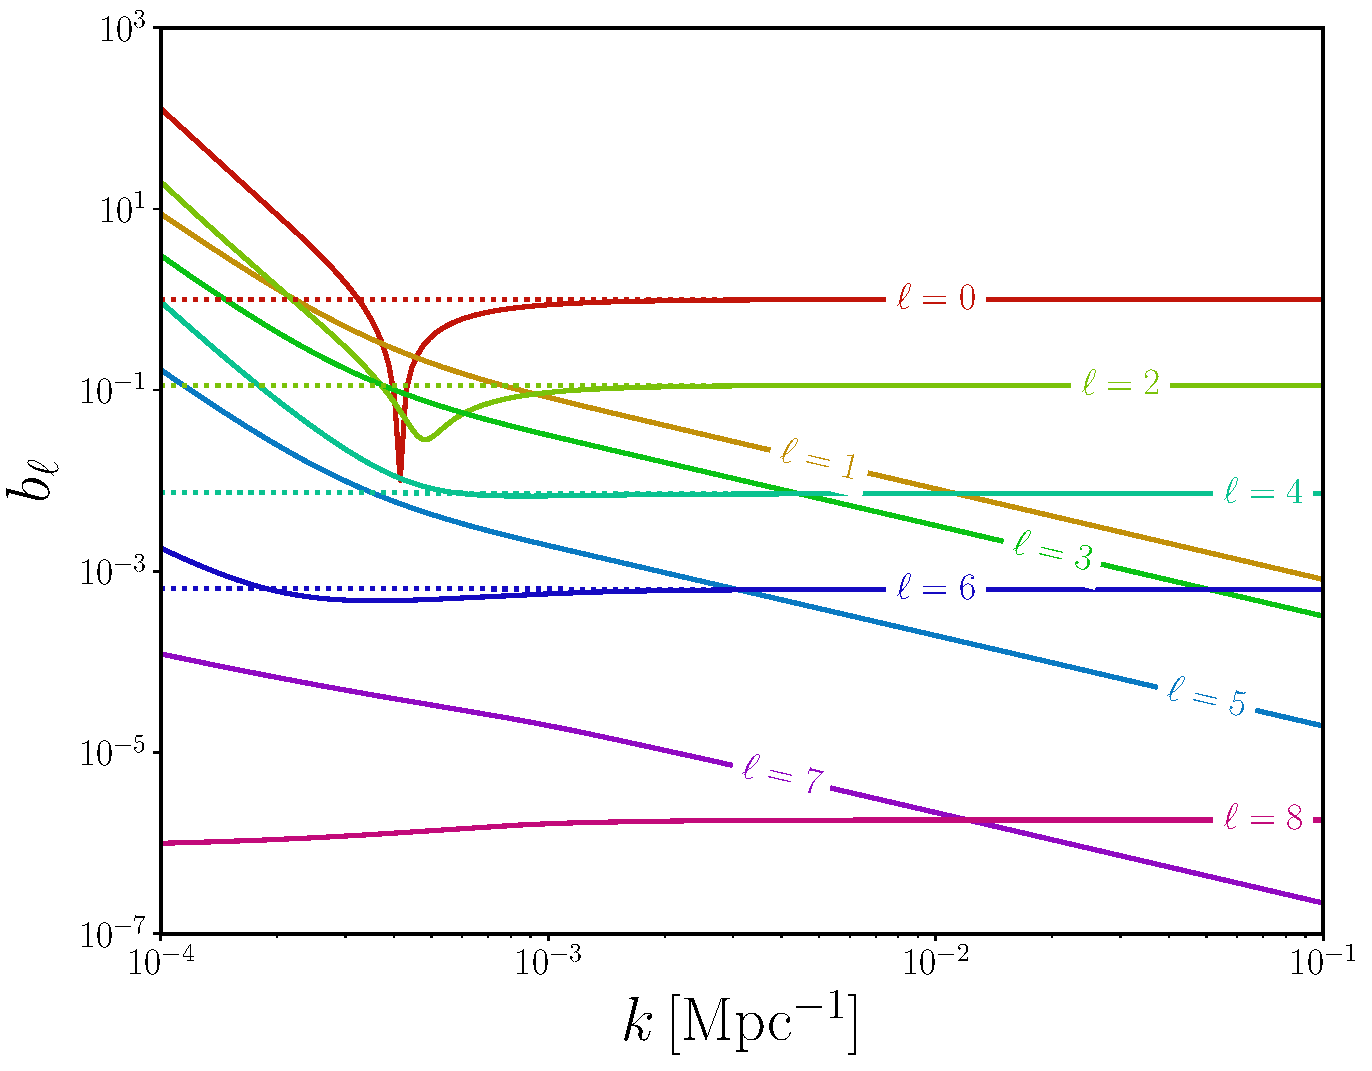
\includegraphics[width=0.85\linewidth]{fig/totP_Euclid_sq2.pdf}
\end{subfigure}%
\begin{subfigure}{0.5\textwidth}
%\centering
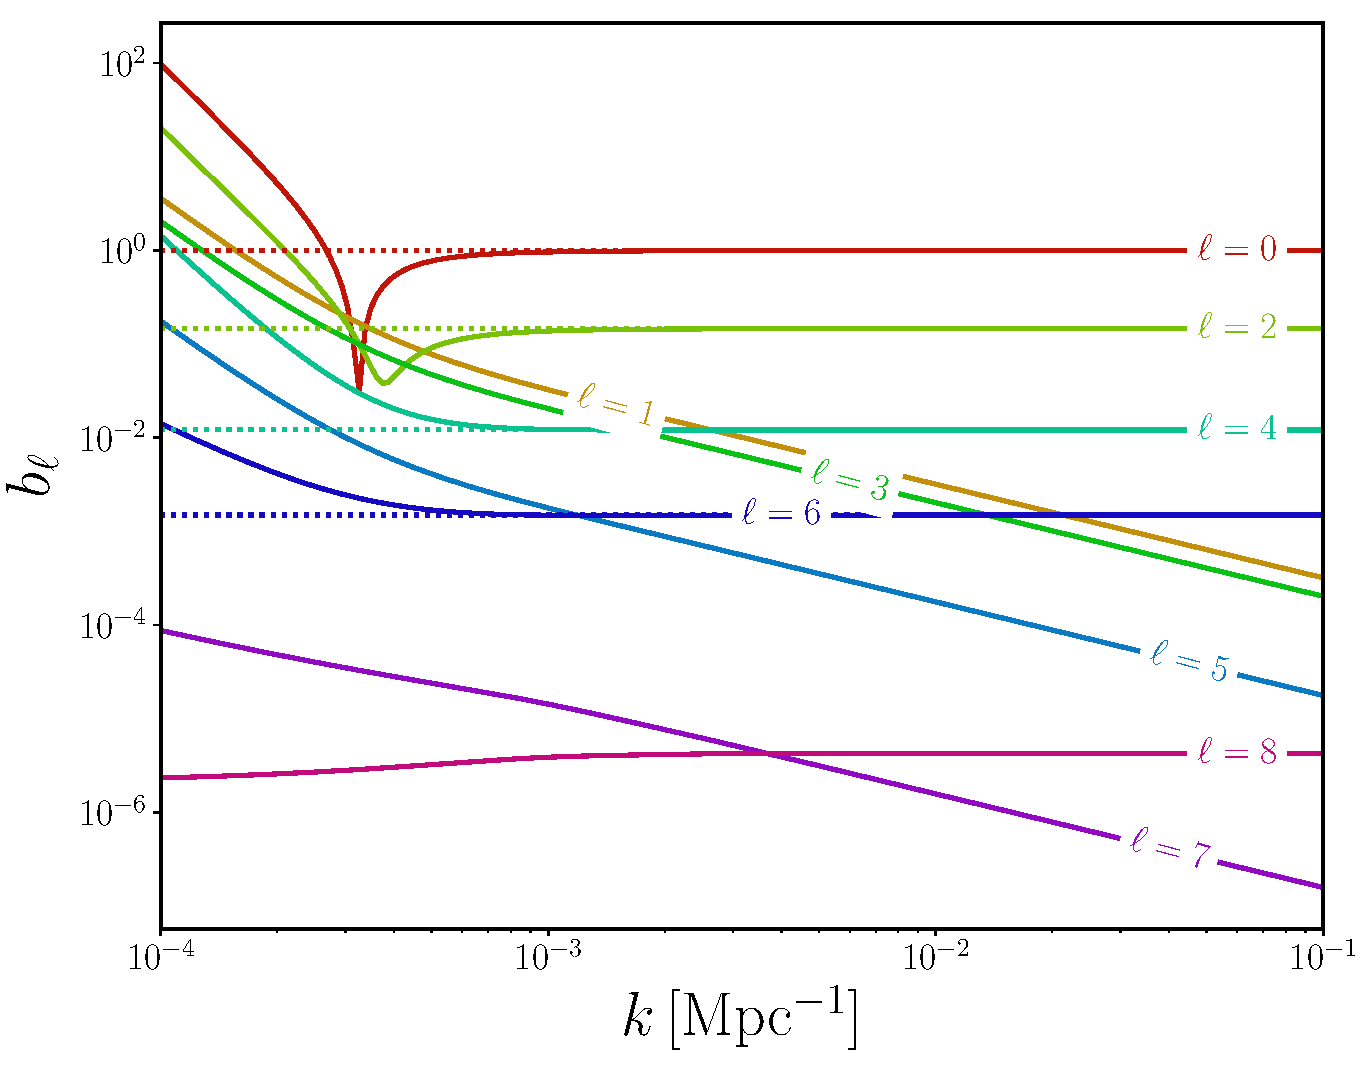
\includegraphics[width=0.85\linewidth]{fig/totP_IM_sq2.pdf}
\end{subfigure}
\caption{Normalised total power for squeezed configuration for Euclid-like (left) and SKA HI intensity mapping (right) surveys. Long mode \(k_3\) is plotted along the \(x\)-axis. \label{fig:totpowersq}}
\end{figure}
\begin{figure}[ht]
%\centering
\begin{subfigure}{0.5\textwidth}
%\centering	
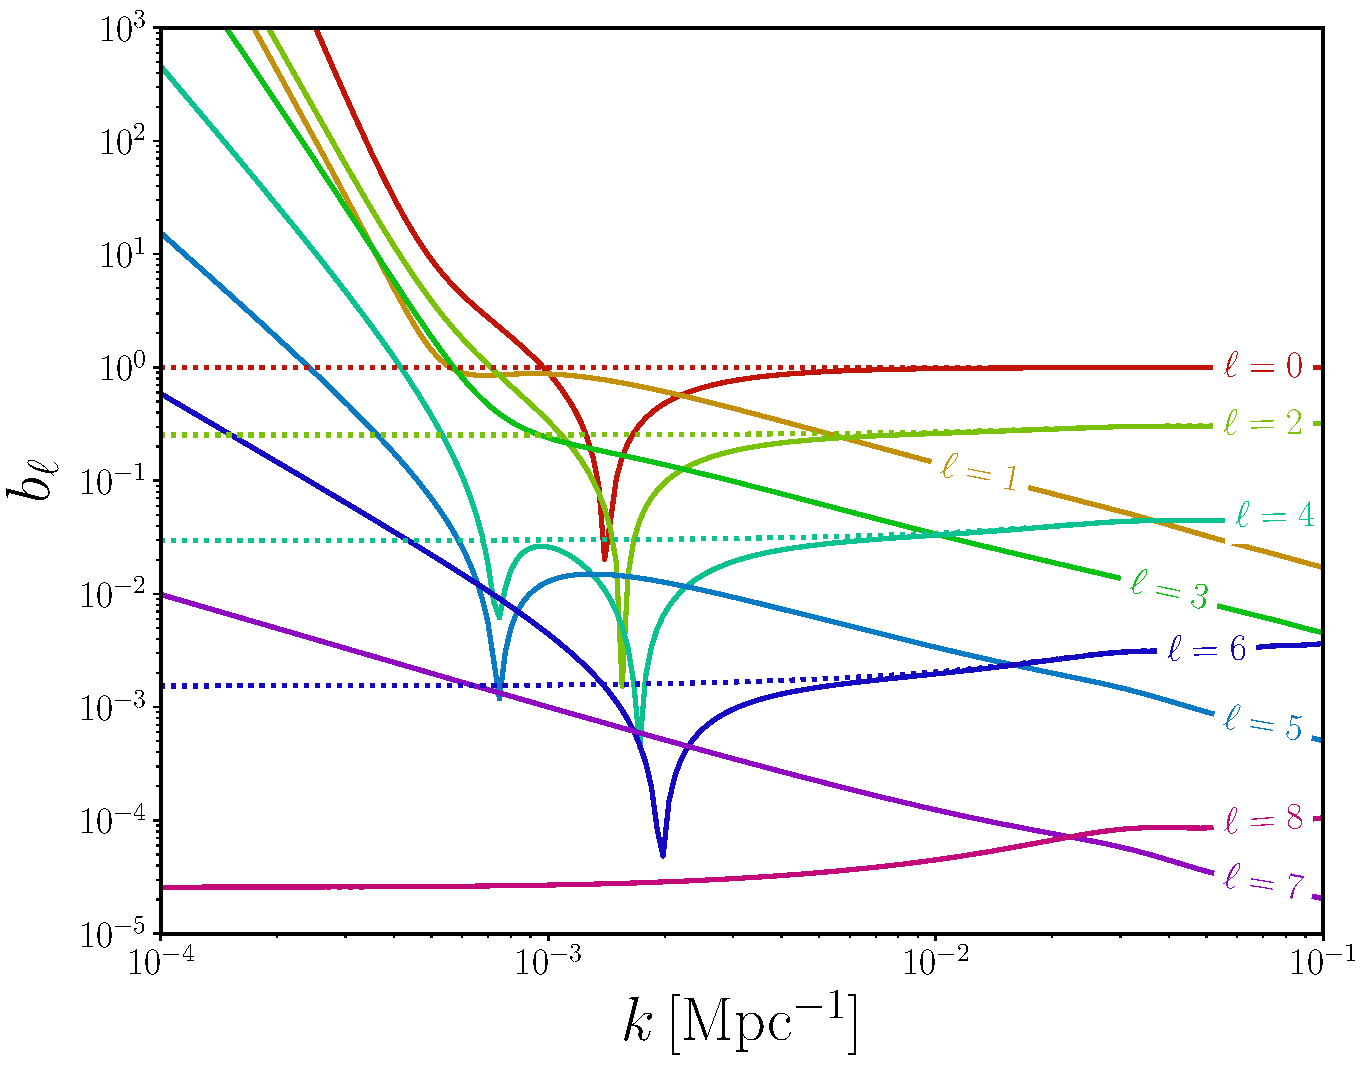
\includegraphics[width=0.85\linewidth]{fig/totP_Euclid_flat2.pdf}
\end{subfigure}%
\begin{subfigure}{0.5\textwidth}
%\centering
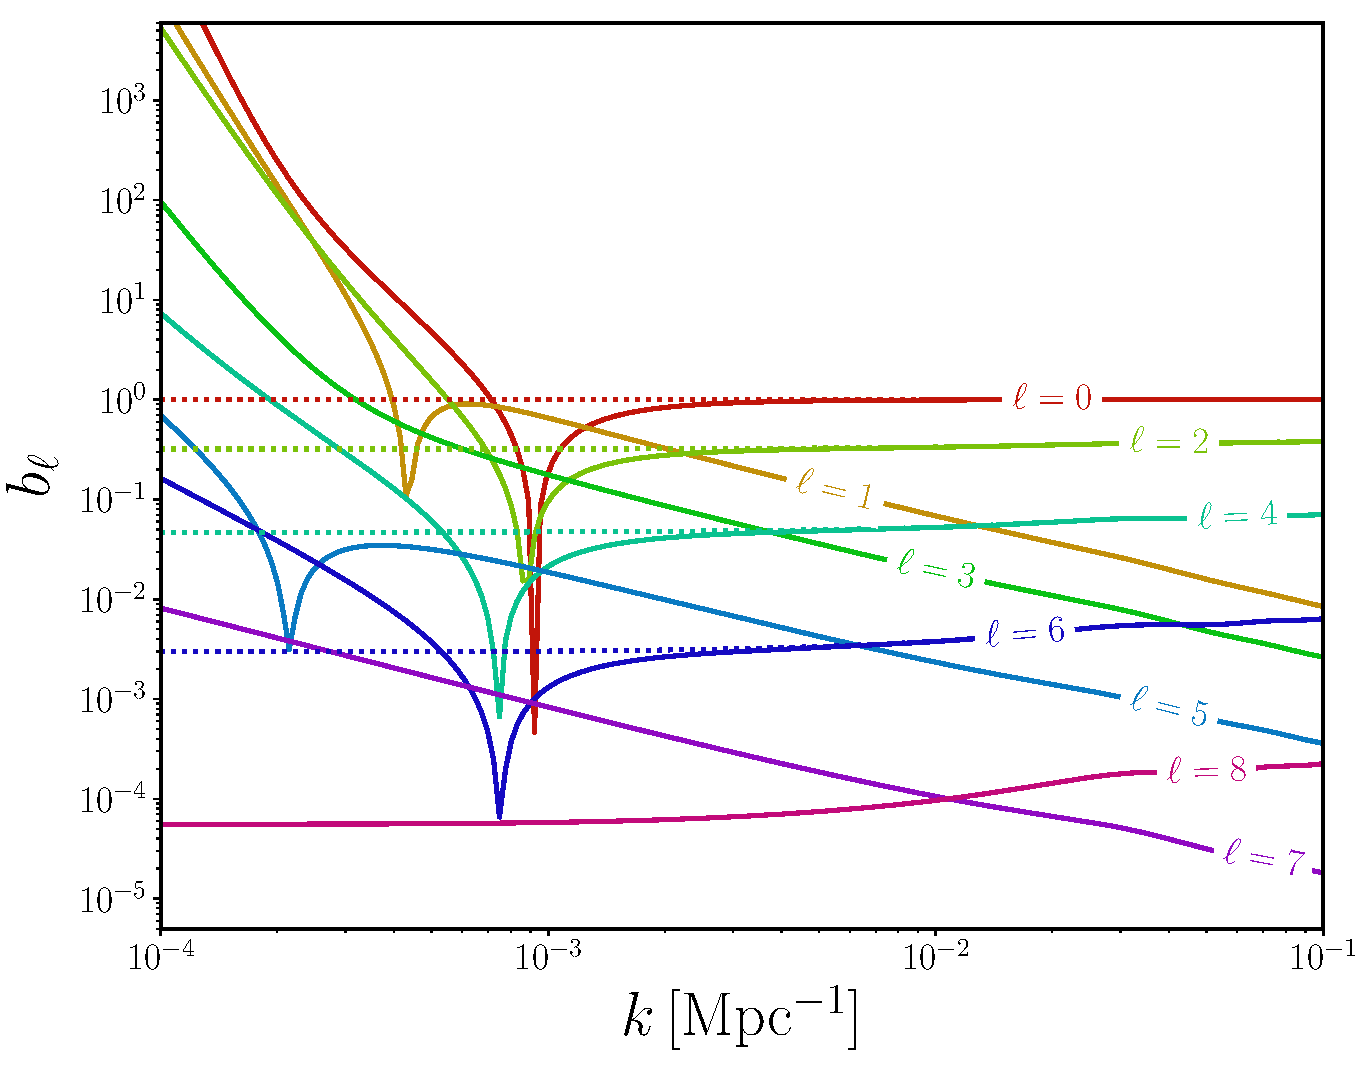
\includegraphics[width=0.85\linewidth]{fig/totP_IM_flat2.pdf}
\end{subfigure}
\caption{Total power for flattened configuration for Euclid-like (left) and SKA HI intensity mapping (right) surveys. Long mode \(k_3\) is plotted along the \(x\)-axis. \label{fig:totpowerfl}}
\end{figure}
\begin{figure}[ht]
%\centering
\begin{subfigure}{0.5\textwidth}
%\centering	
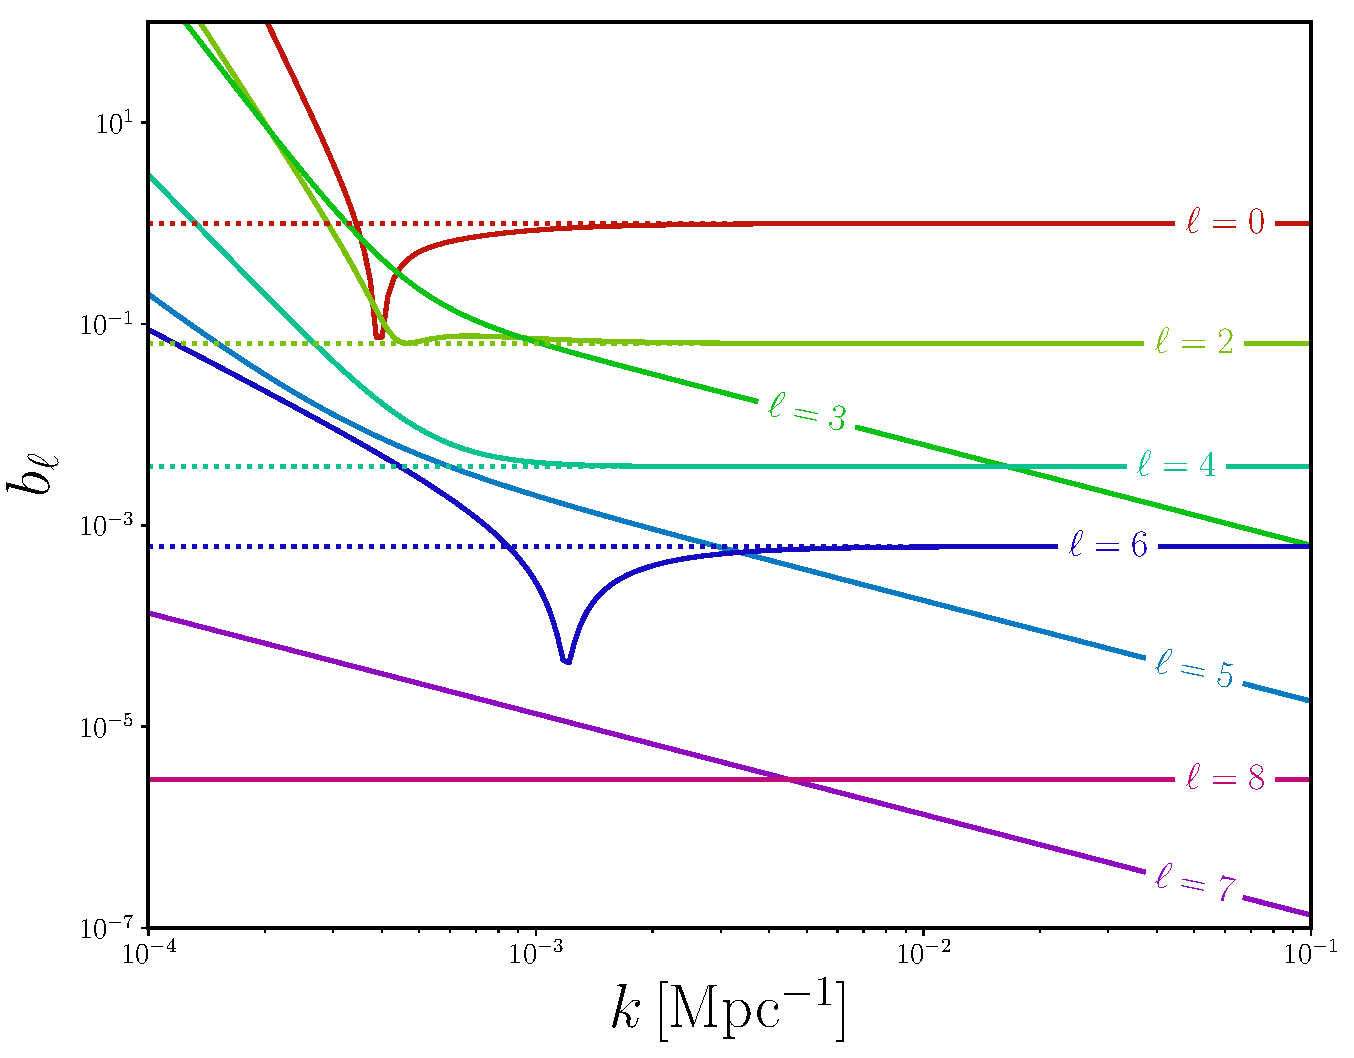
\includegraphics[width=0.85\linewidth]{fig/totP_euclid_equi2.pdf}
\end{subfigure}%
\begin{subfigure}{0.5\textwidth}
%\centering
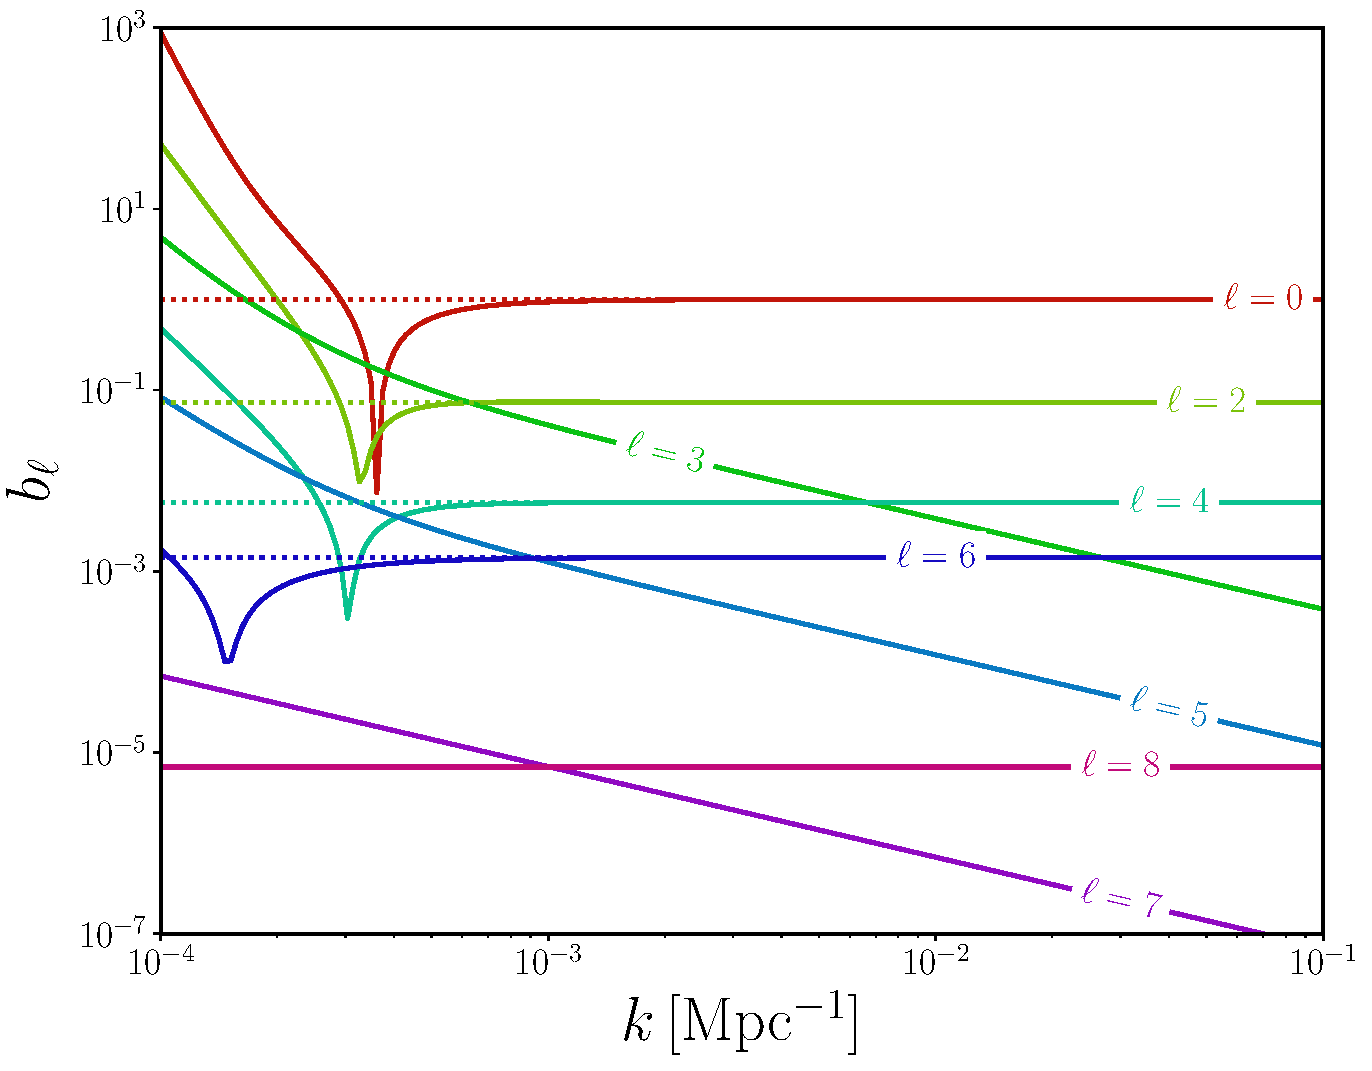
\includegraphics[width=0.85\linewidth]{fig/totP_IM_equi2.pdf}
\end{subfigure}
\caption{Total power for equilateral configuration for Euclid-like (left) and SKA HI intensity mapping (right) surveys. Since the dipole vanishes in this limit, the \(\ell = 1\) line is absent.\label{fig:totpowereq}}
\end{figure}


\clearpage
\begin{figure}[ht]
\centering
    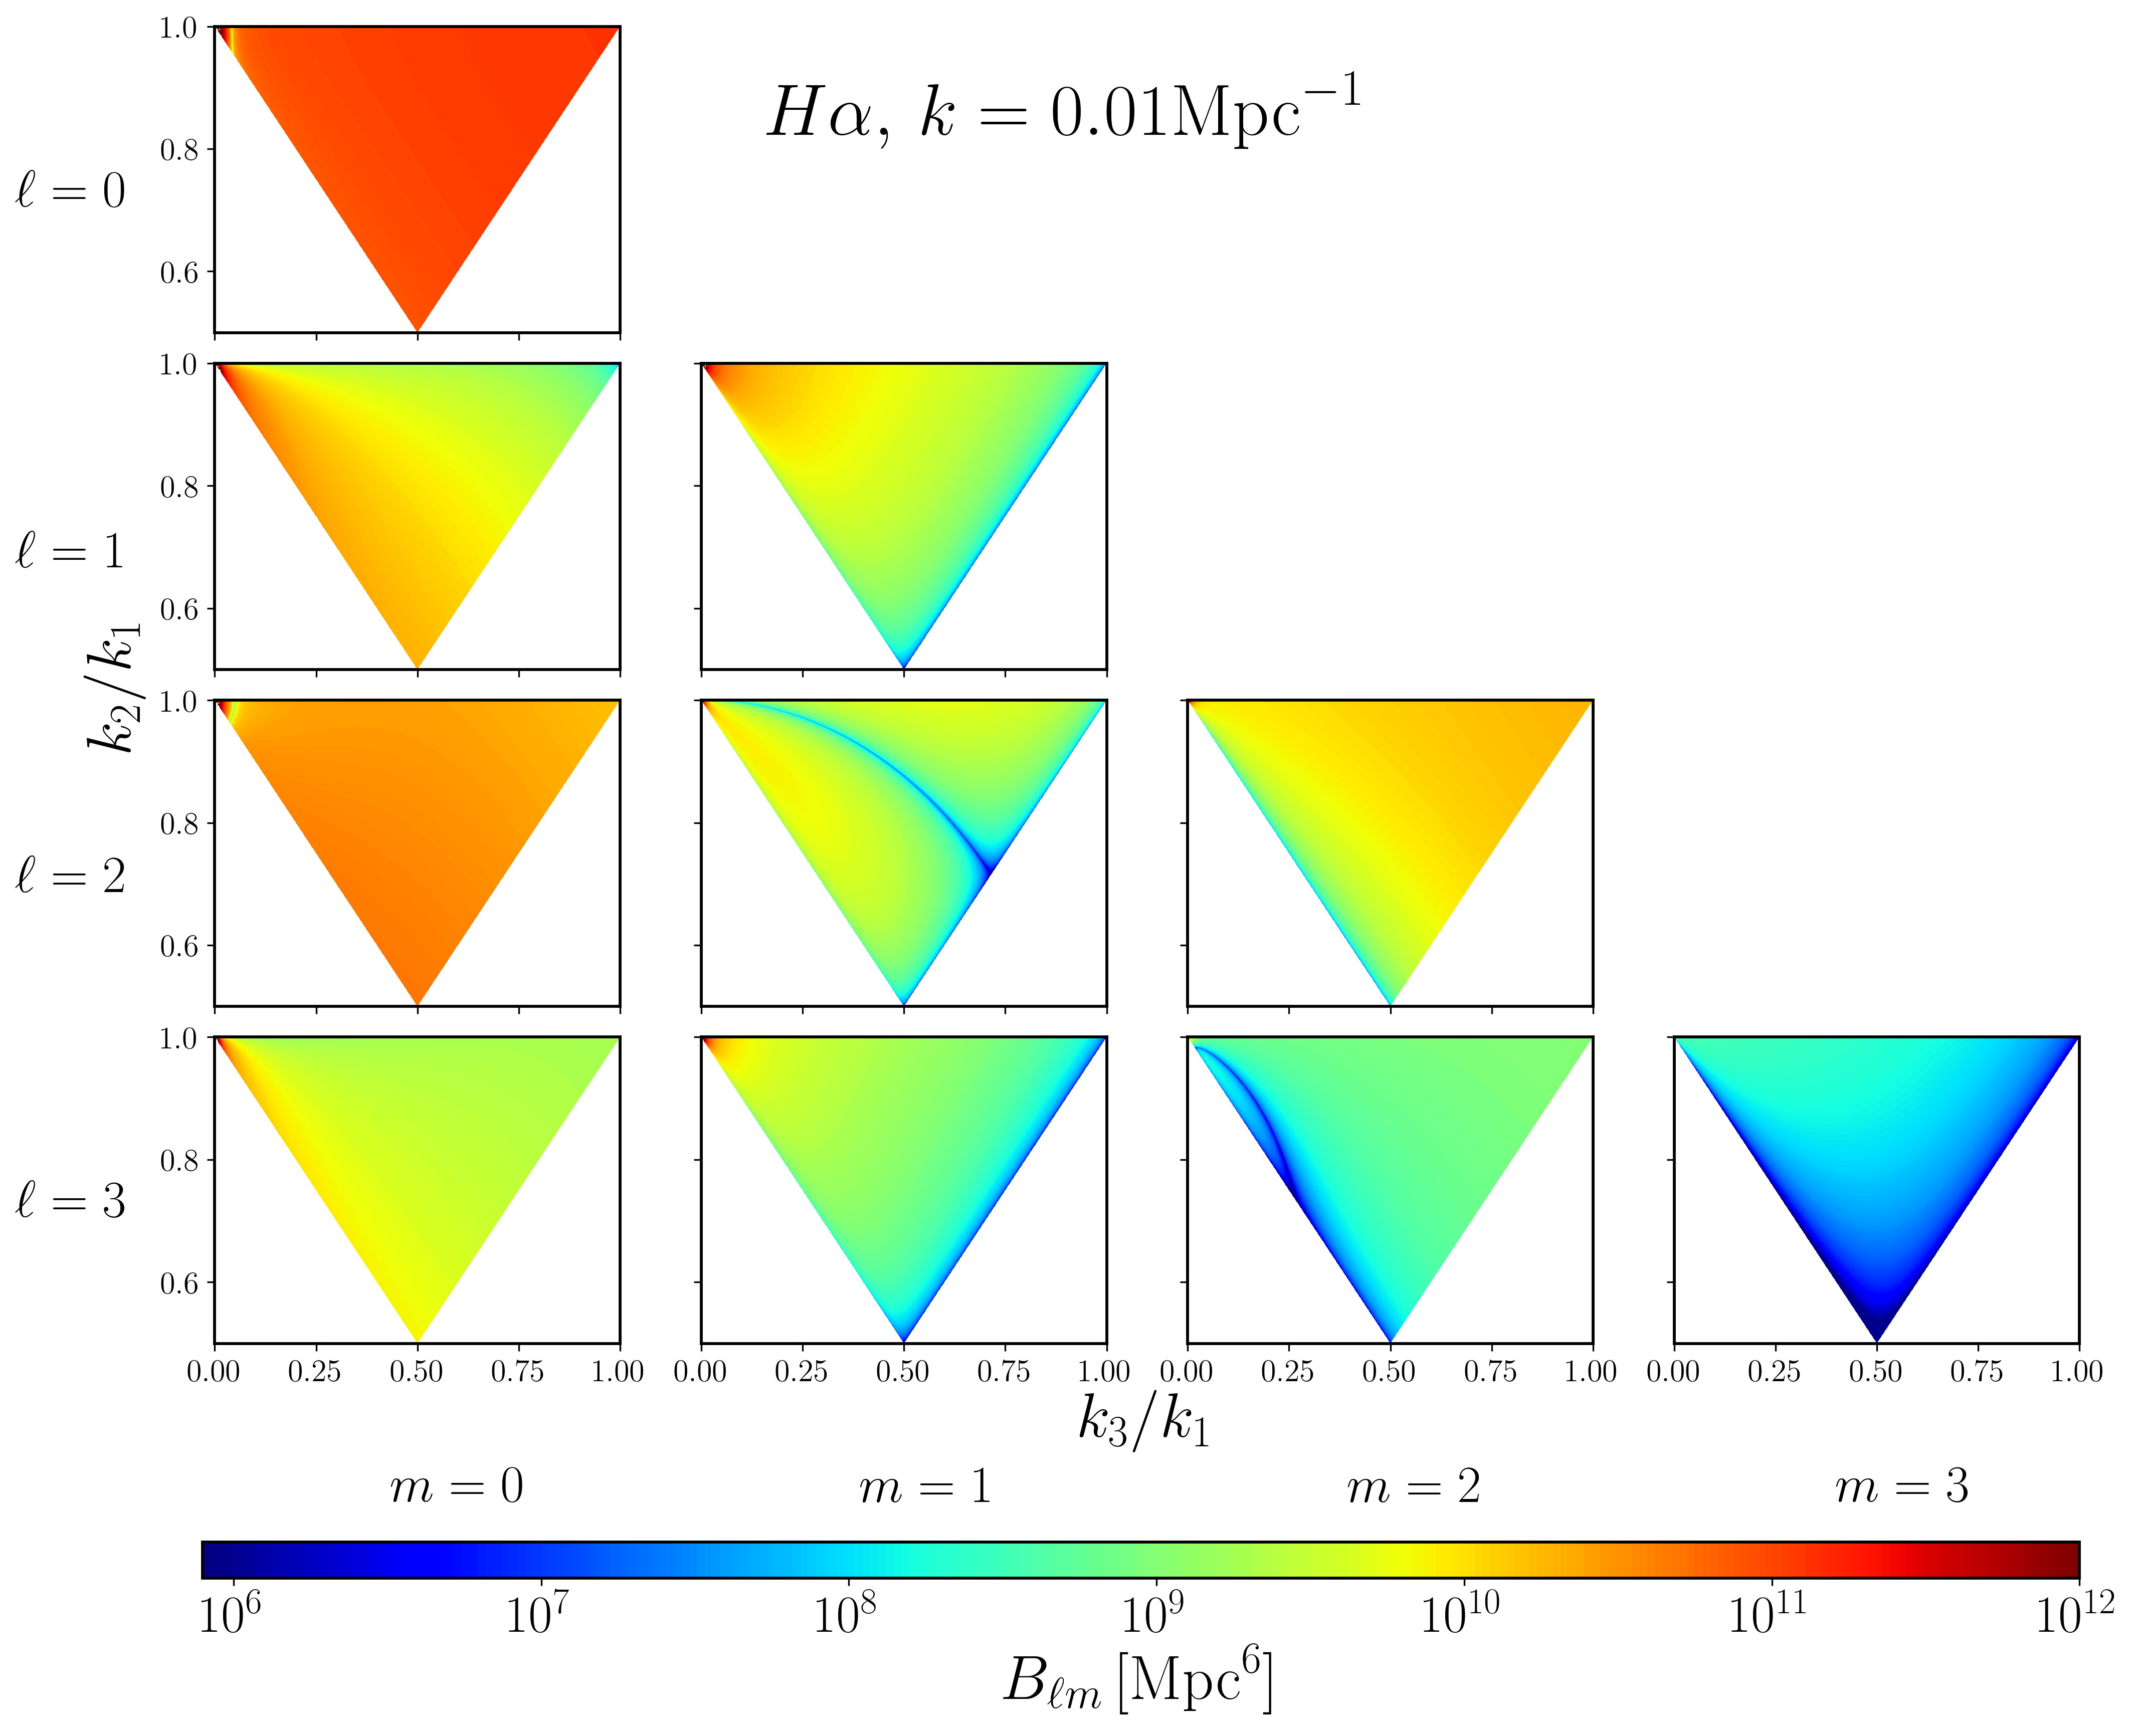
\includegraphics[width=0.7\textwidth]{fig/triangles_all_k001_Euclid.png}
	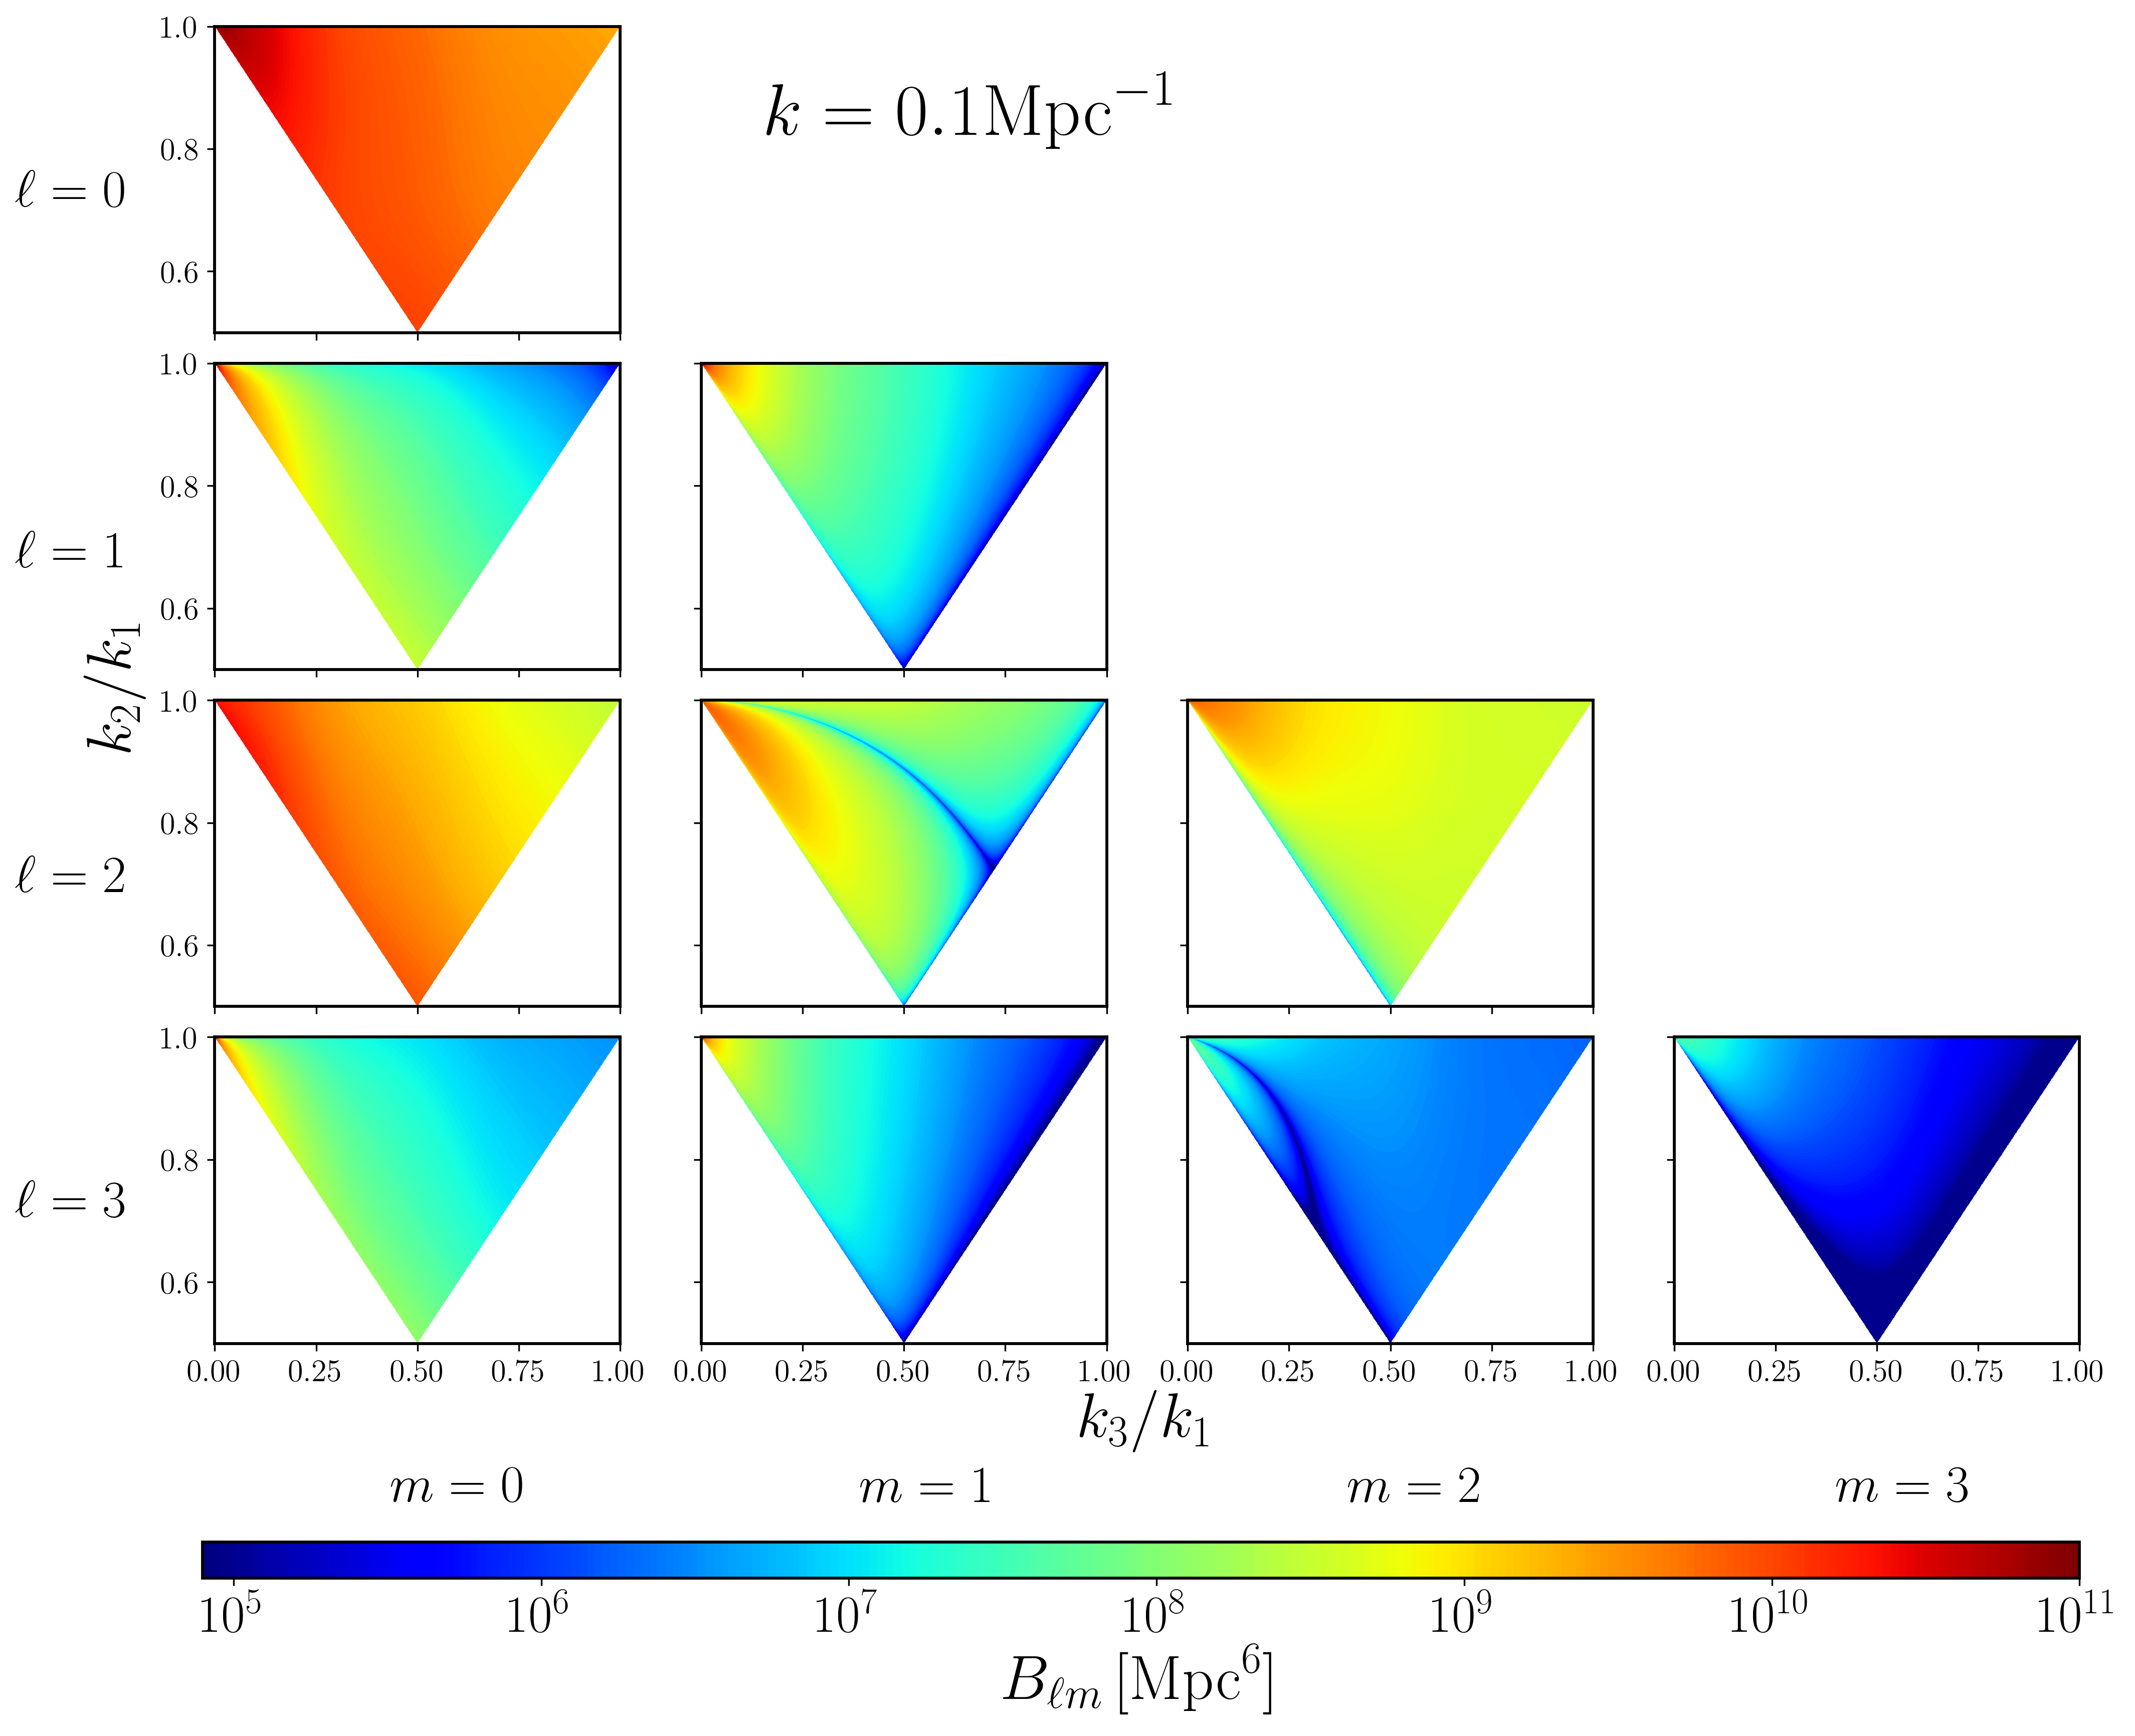
\includegraphics[width=0.7\textwidth]{fig/triangles_all_k01_Euclid.png}
	\caption{A selection of multipoles of the galaxy bispectrum, \(B_{\ell m}\), with \(\ell = 0 \ldots 3\) and \(m = 0 \ldots \ell\) as indicated in the figure. Bias model used is that for \(H\alpha\)/Euclid-like survey. \(k_1\) is kept fixed, the value of which is given alongside the plot, and the \(x\) and \(y\) axes vary respectively \(k_3\) and \(k_2\) with respect to the fixed \(k_1\). The upper left corner of the wedge shape is the squeezed limit, the upper right corner is the equilateral configuration, and the lower corner is the co-linear configuration. Note the difference in range of the colour bars.}
		\label{fig:euclidtriangle}
\end{figure}

\clearpage
\begin{figure}[ht]
	\centering
	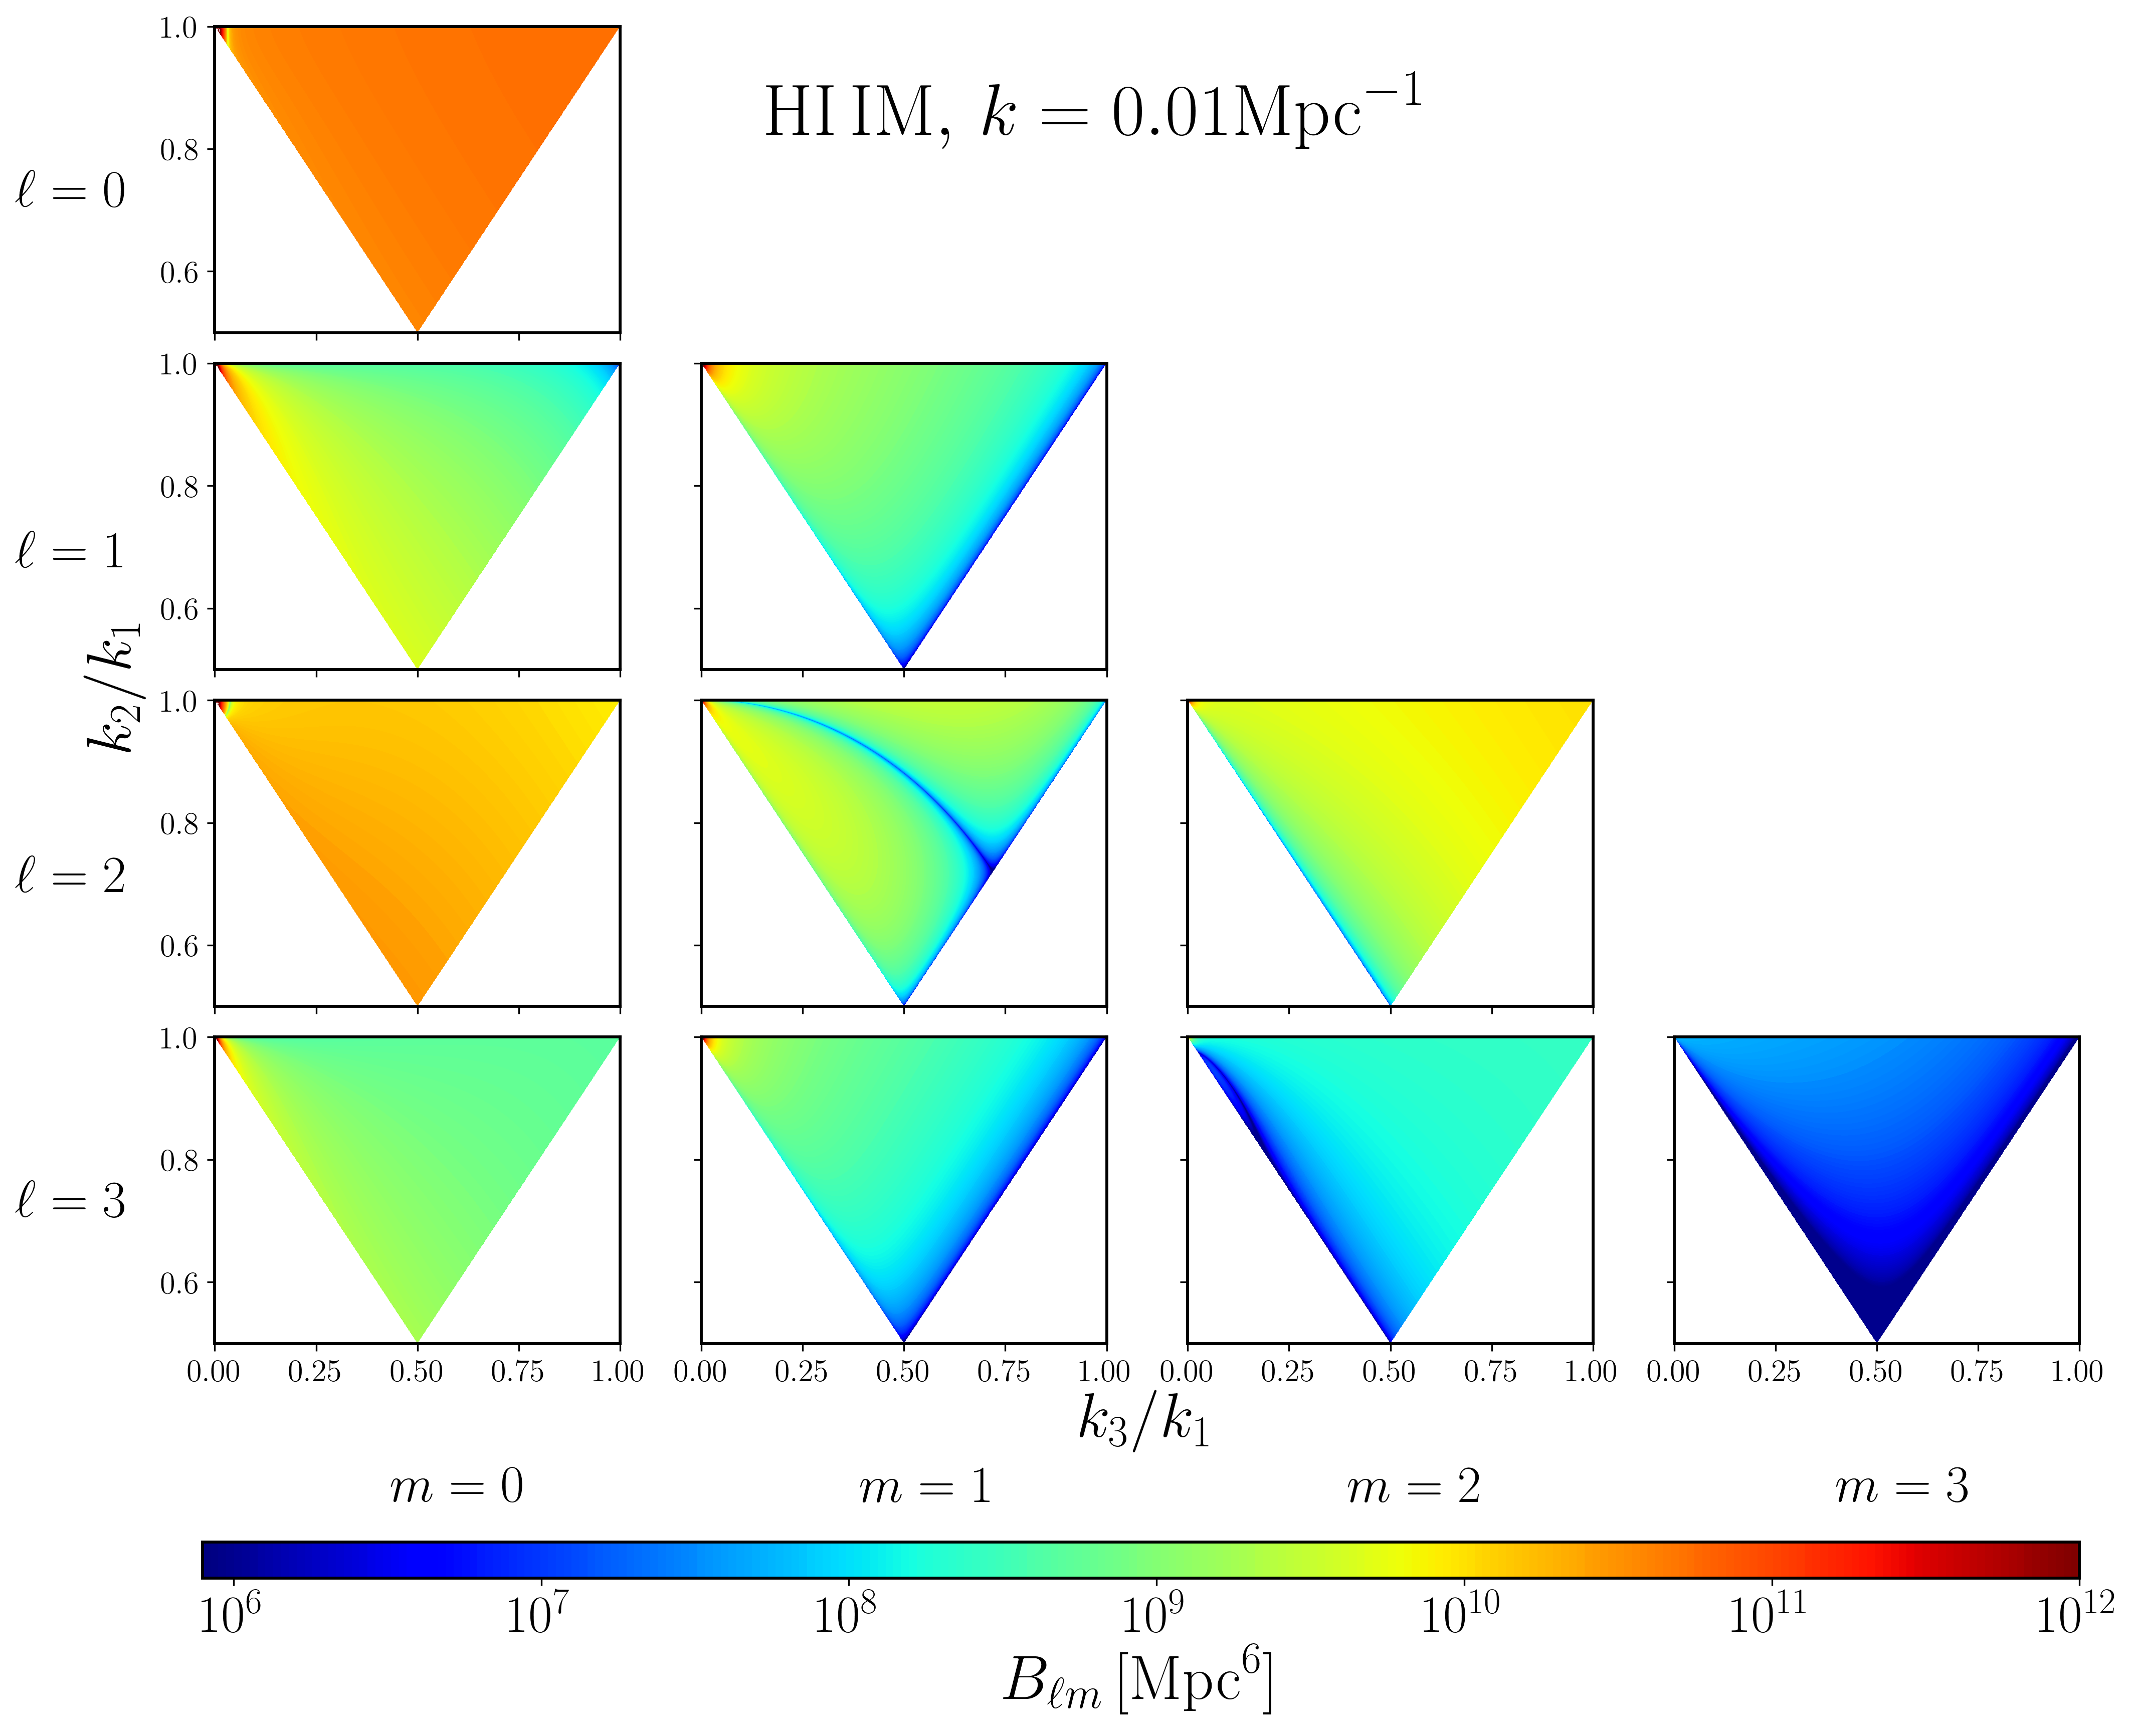
\includegraphics[width=0.8\textwidth]{fig/triangles_all_k001_IM.png}
	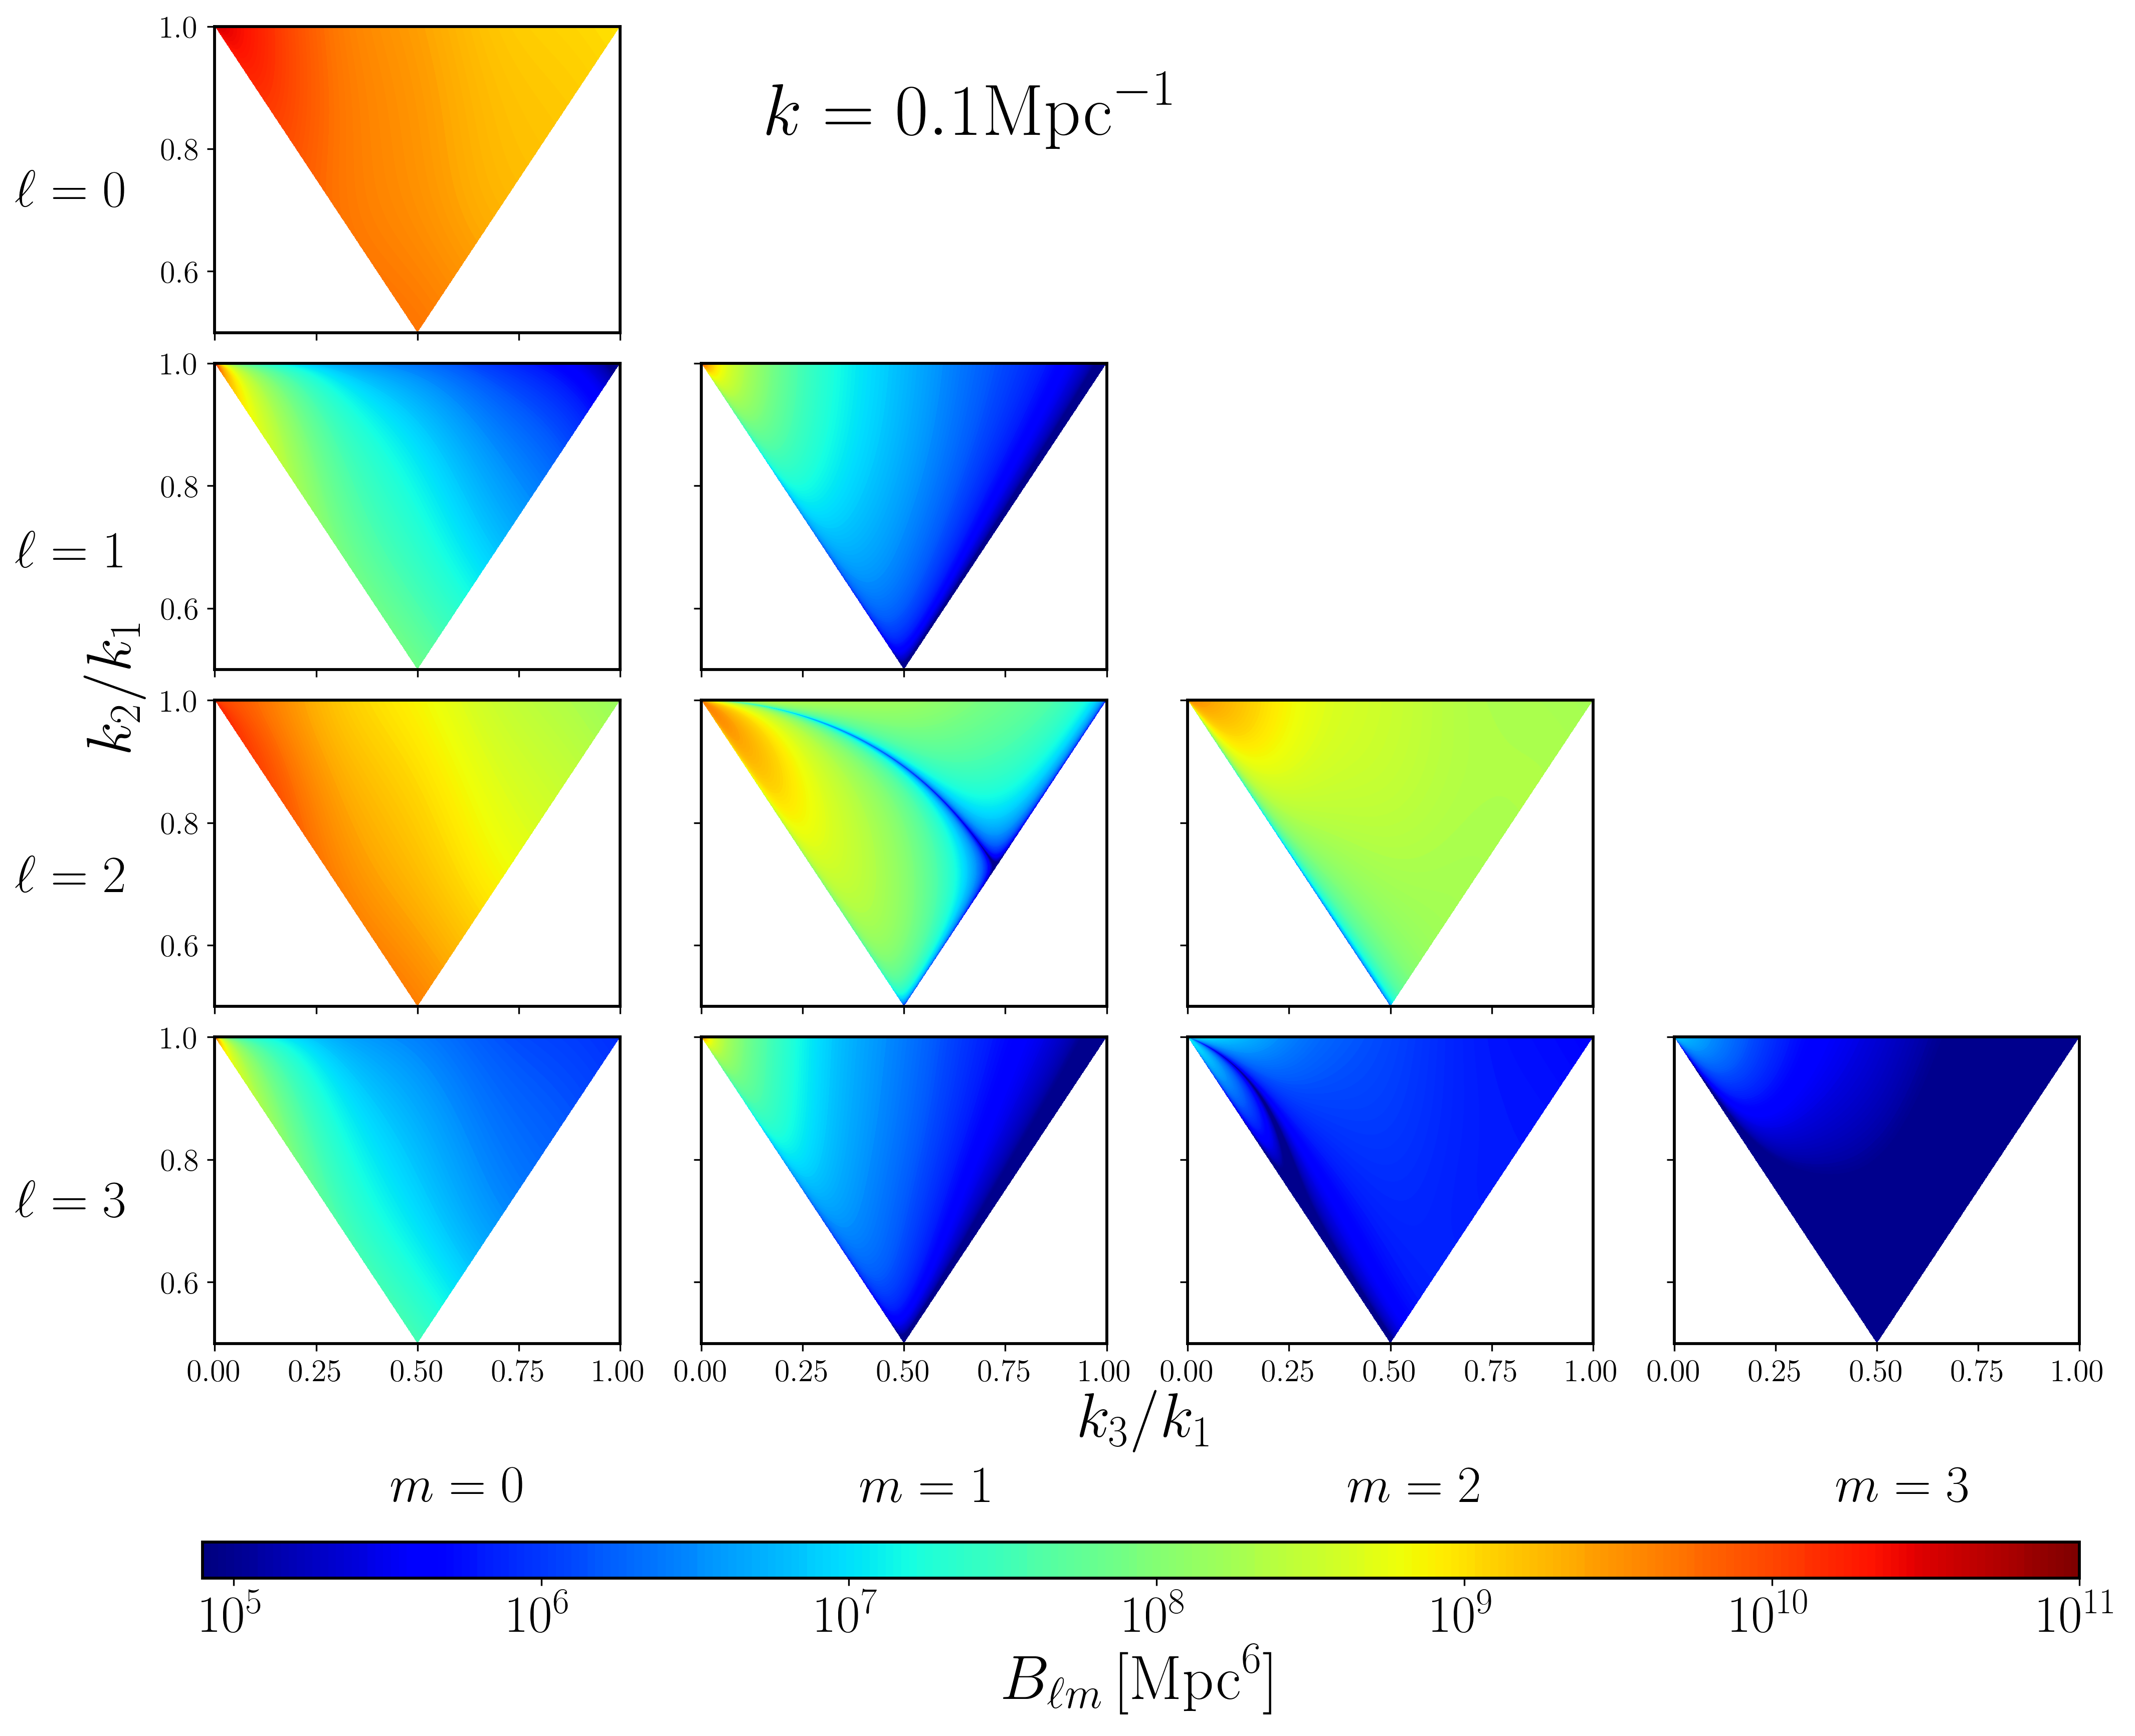
\includegraphics[width=0.8\textwidth]{fig/triangles_all_k01_IM.png} 
	\caption{Selected multipoles of the galaxy bispectrum, similar to figure~\ref{fig:euclidtriangle}, but with the bias model appropriate for intensity mapping. The value of fixed \(k_1\) is indicated on the figures. The upper left corner of a wedge shape is the squeezed limit, the upper right corner is the equilateral configuration, and the lower corner is the co-linear configuration. \label{fig:imtriangle}}
\end{figure}

\clearpage
\begin{figure}[ht]
	\centering
	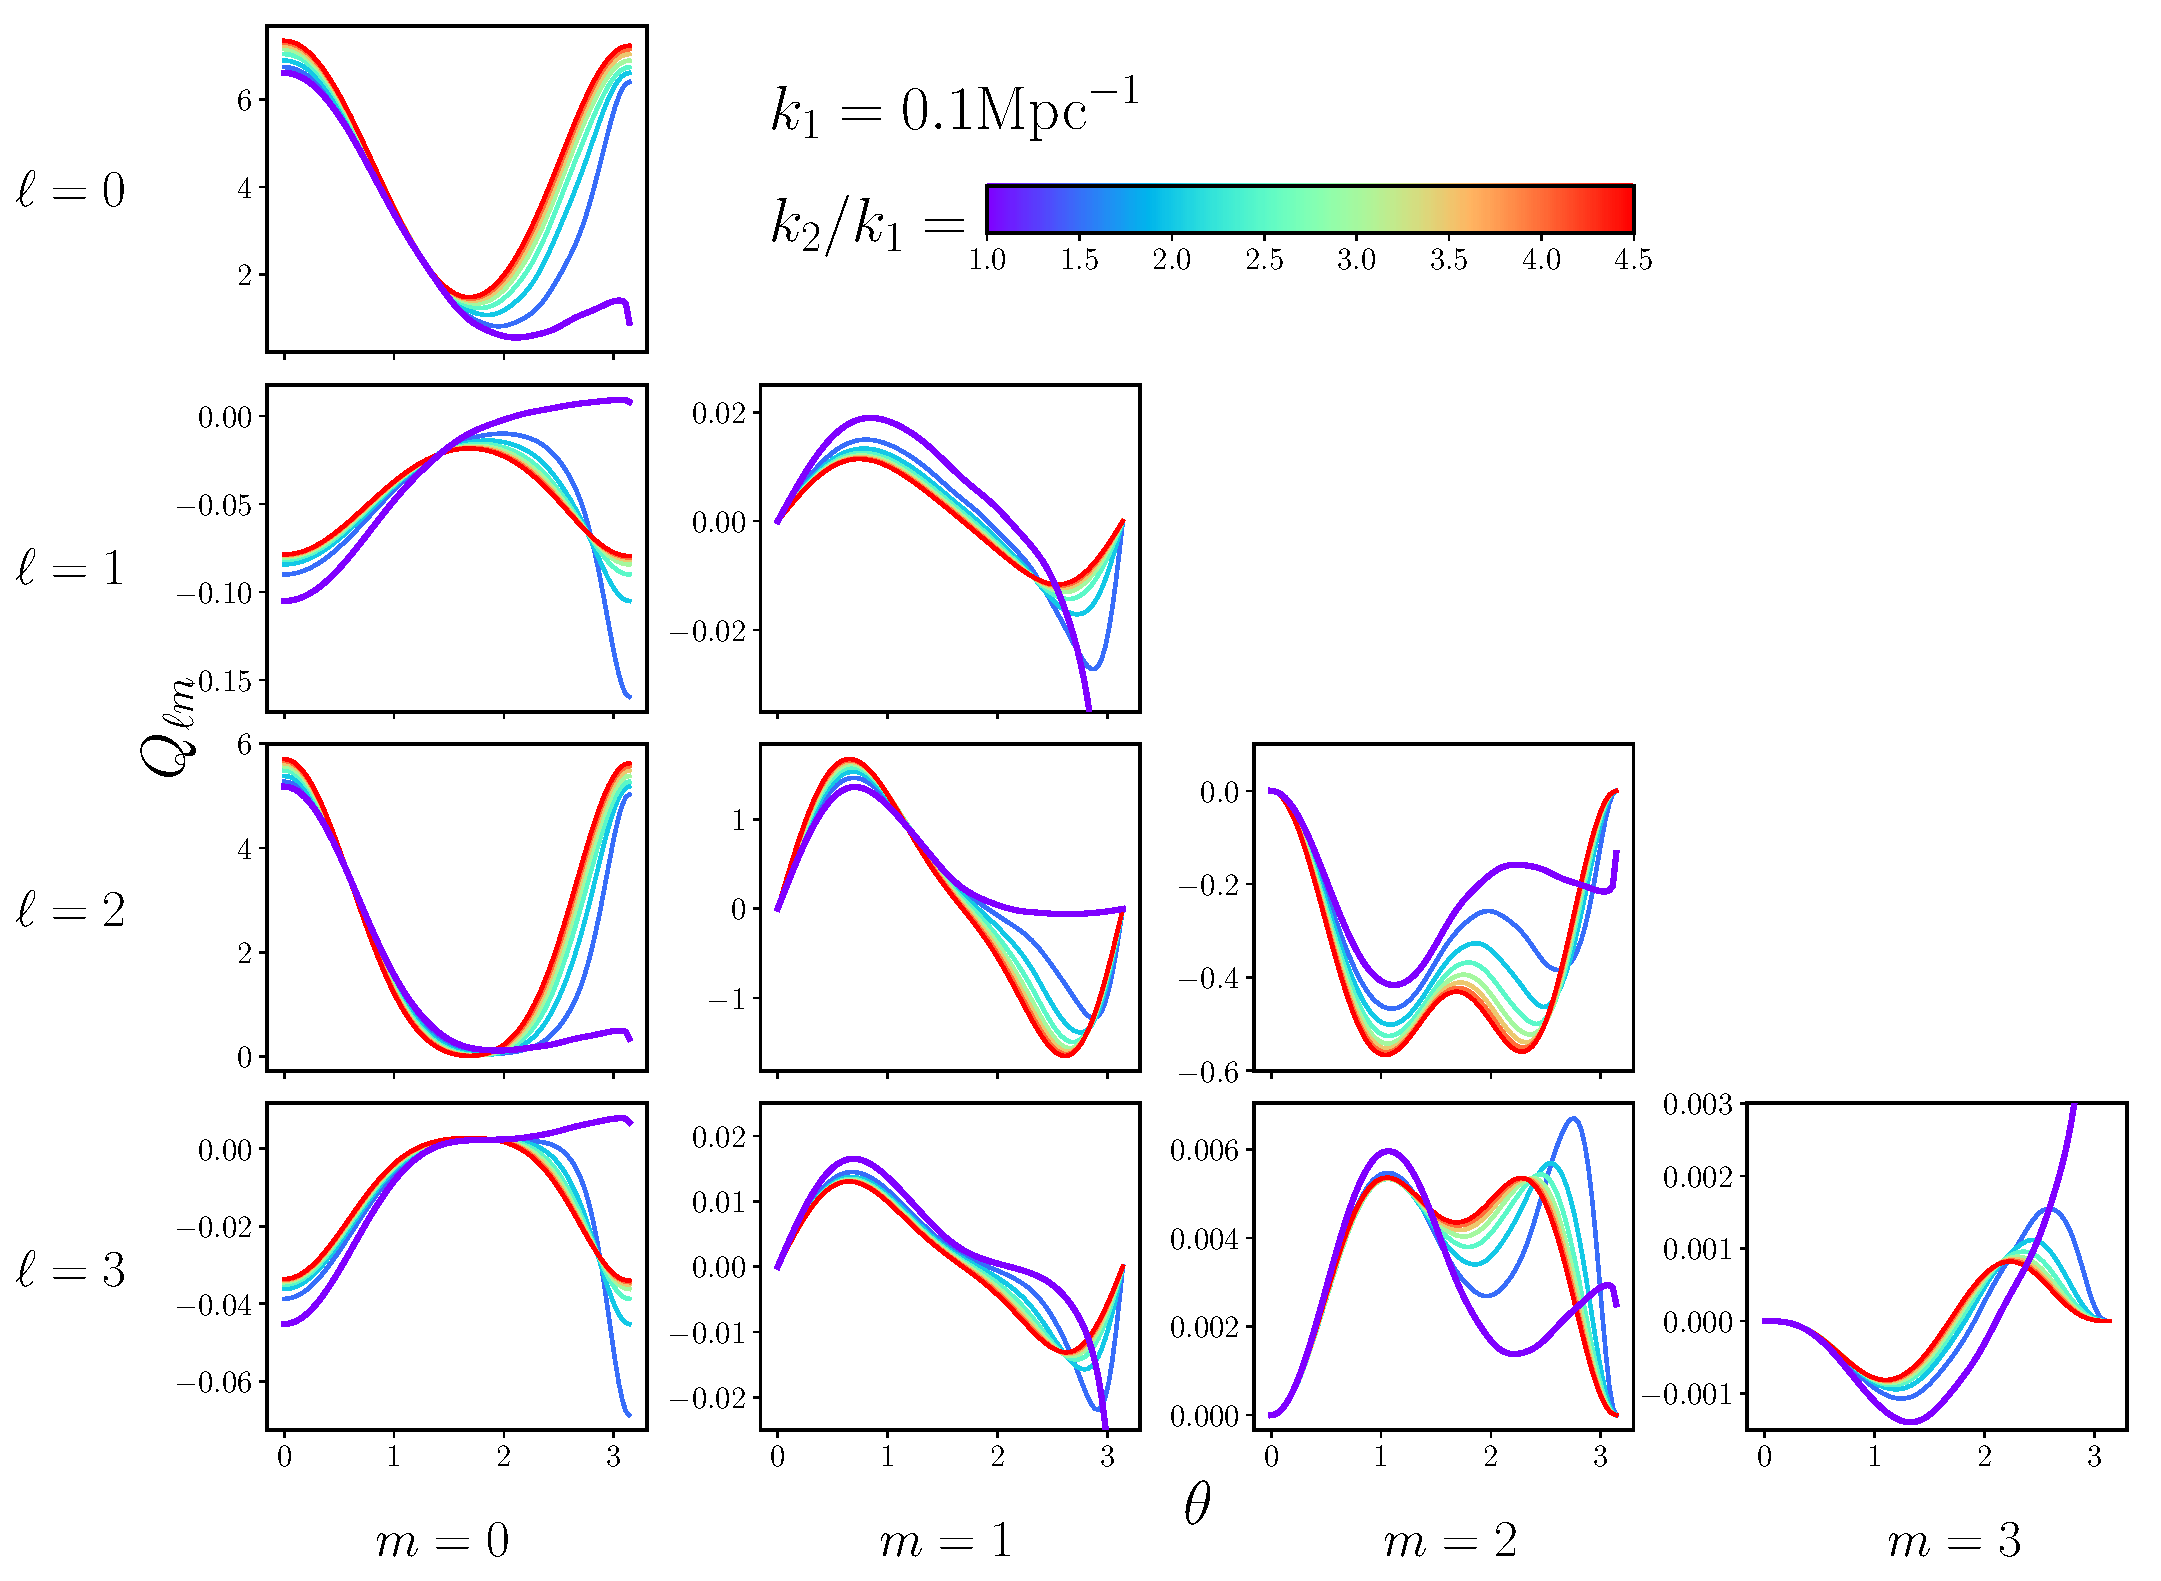
\includegraphics[width=0.85\linewidth]{fig/redB_k01.pdf}
	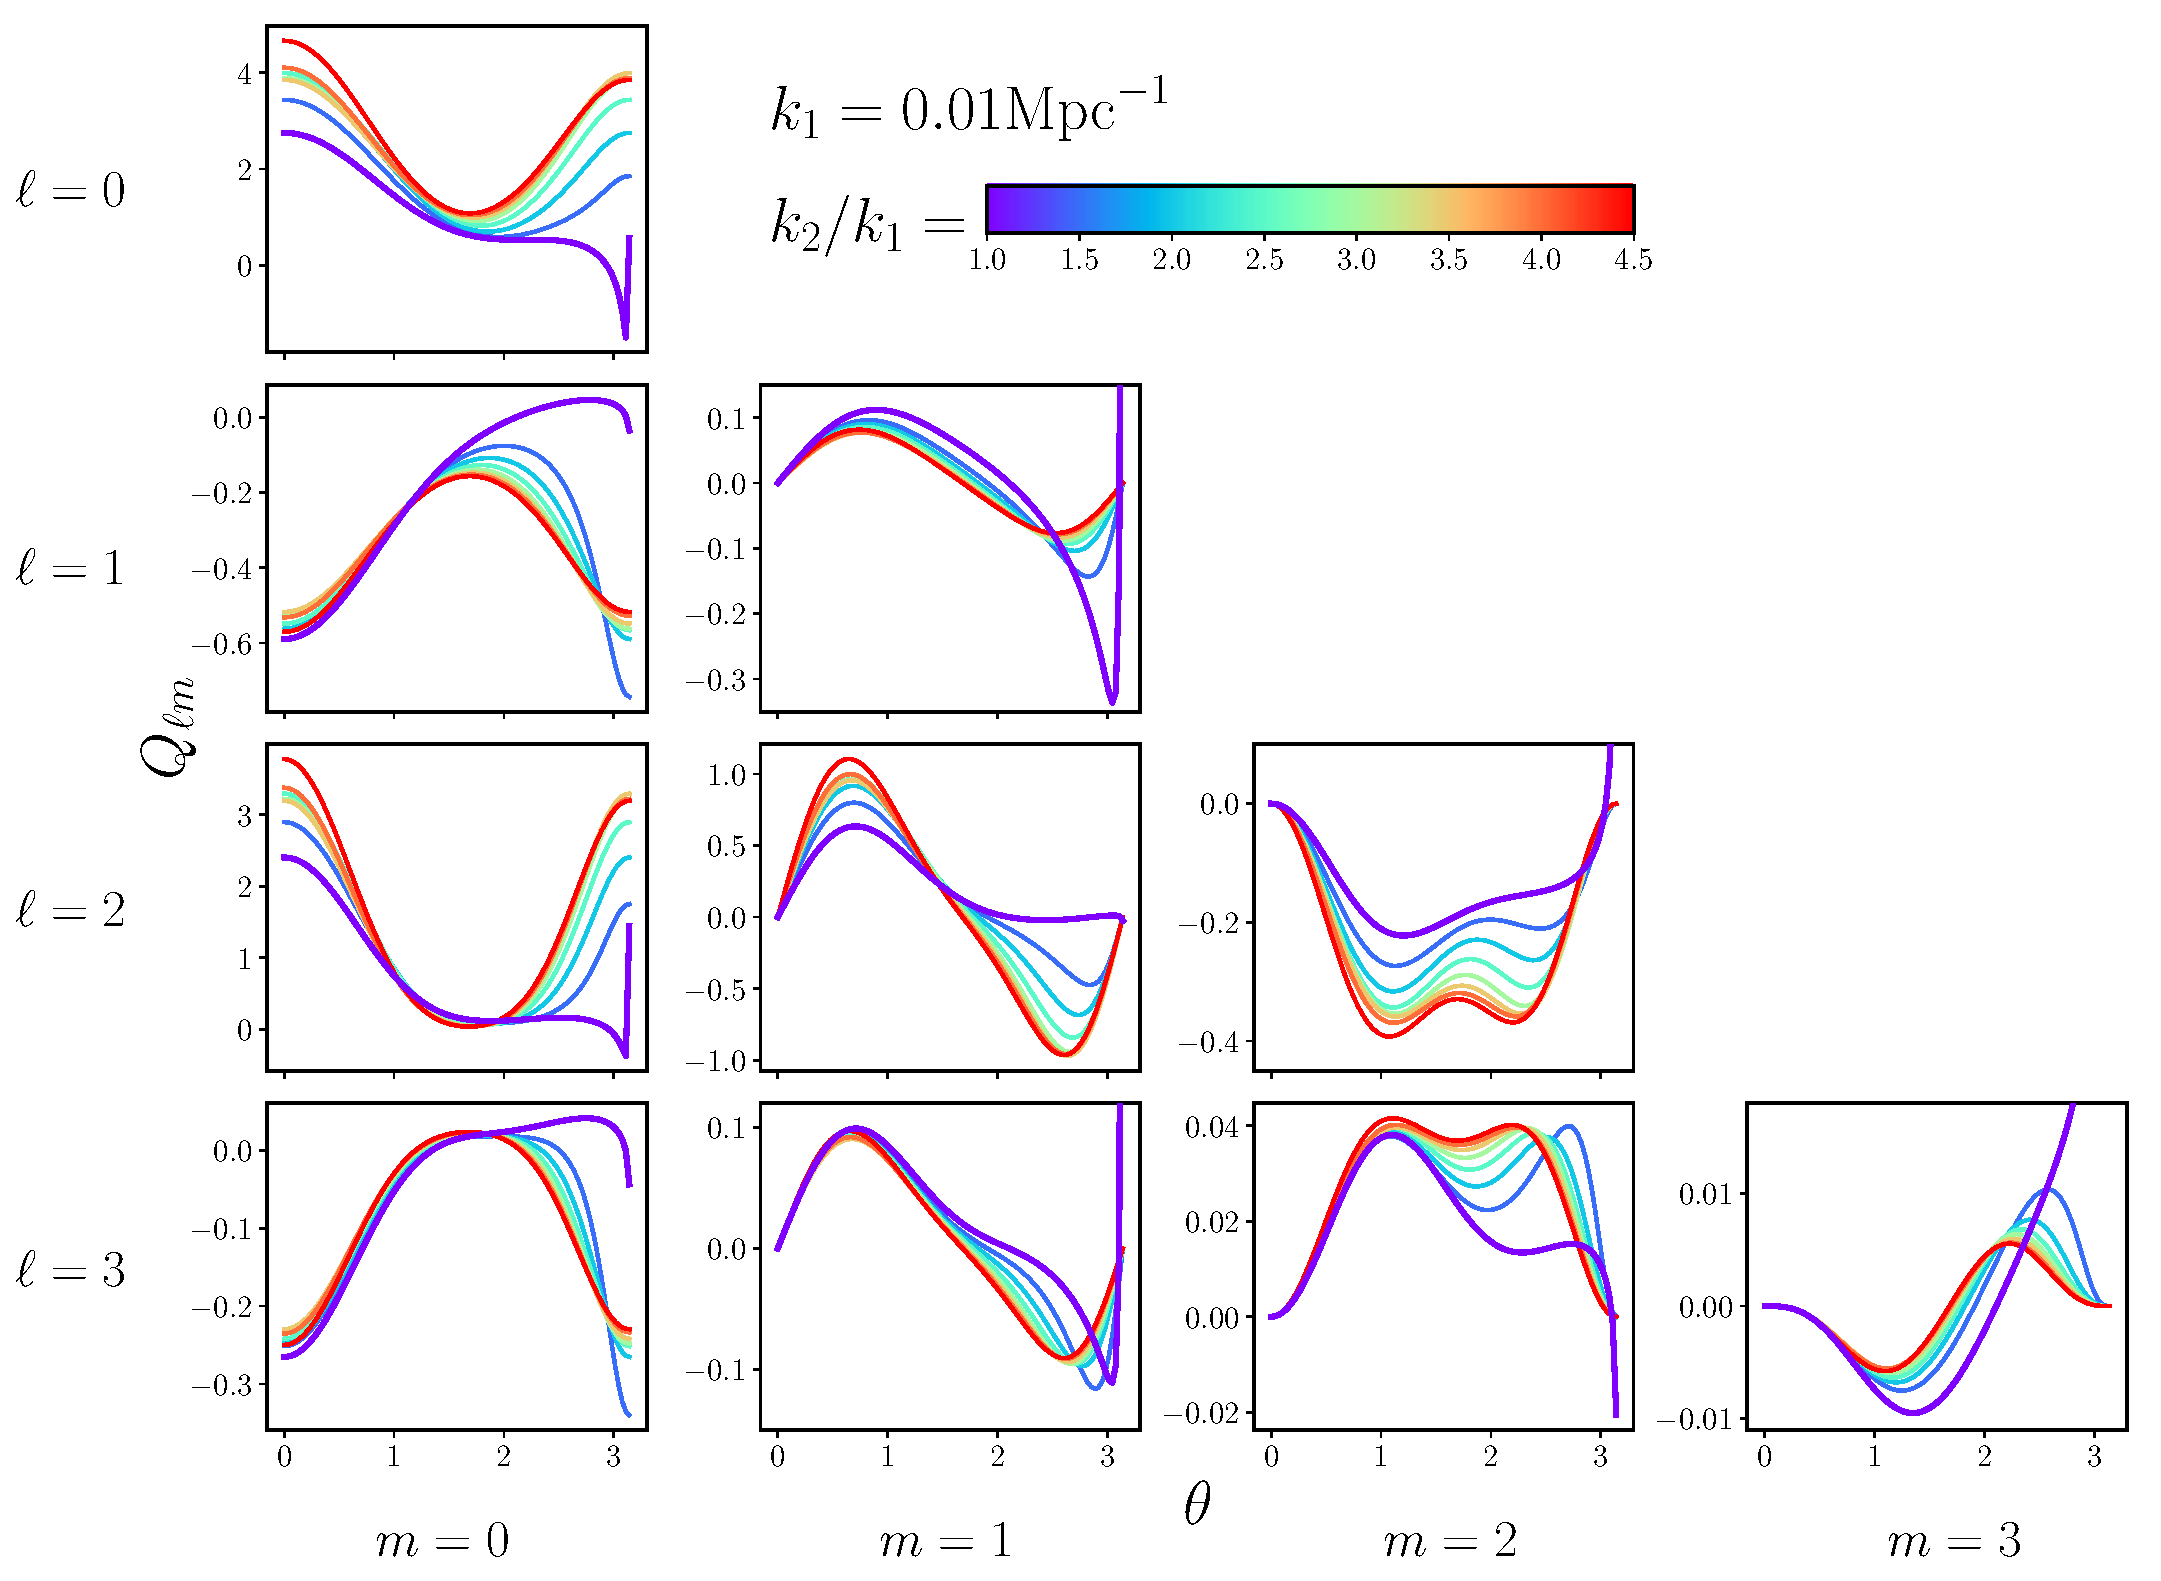
\includegraphics[width=0.85\linewidth]{fig/redB_k001.pdf}
	\caption{Results for the reduced bispectrum \(Q_{\ell m}\), where \(\ell = 0 \ldots 3\) and negative \(m\) not shown. The multipoles \(\ell,m\) are indicated on the figure, as well as the value of \(k_1\) which is kept fixed. The colourbar and different colours denote the ratio of \(k_2/k_1\), where the slightly thicker purple line is the isosceles triangle, which diverges as \(\theta\to\pi\) since there \(k_3\to 0\). \label{fig:Q_rb}}
\end{figure}

\clearpage
\begin{figure}[ht]
\centering
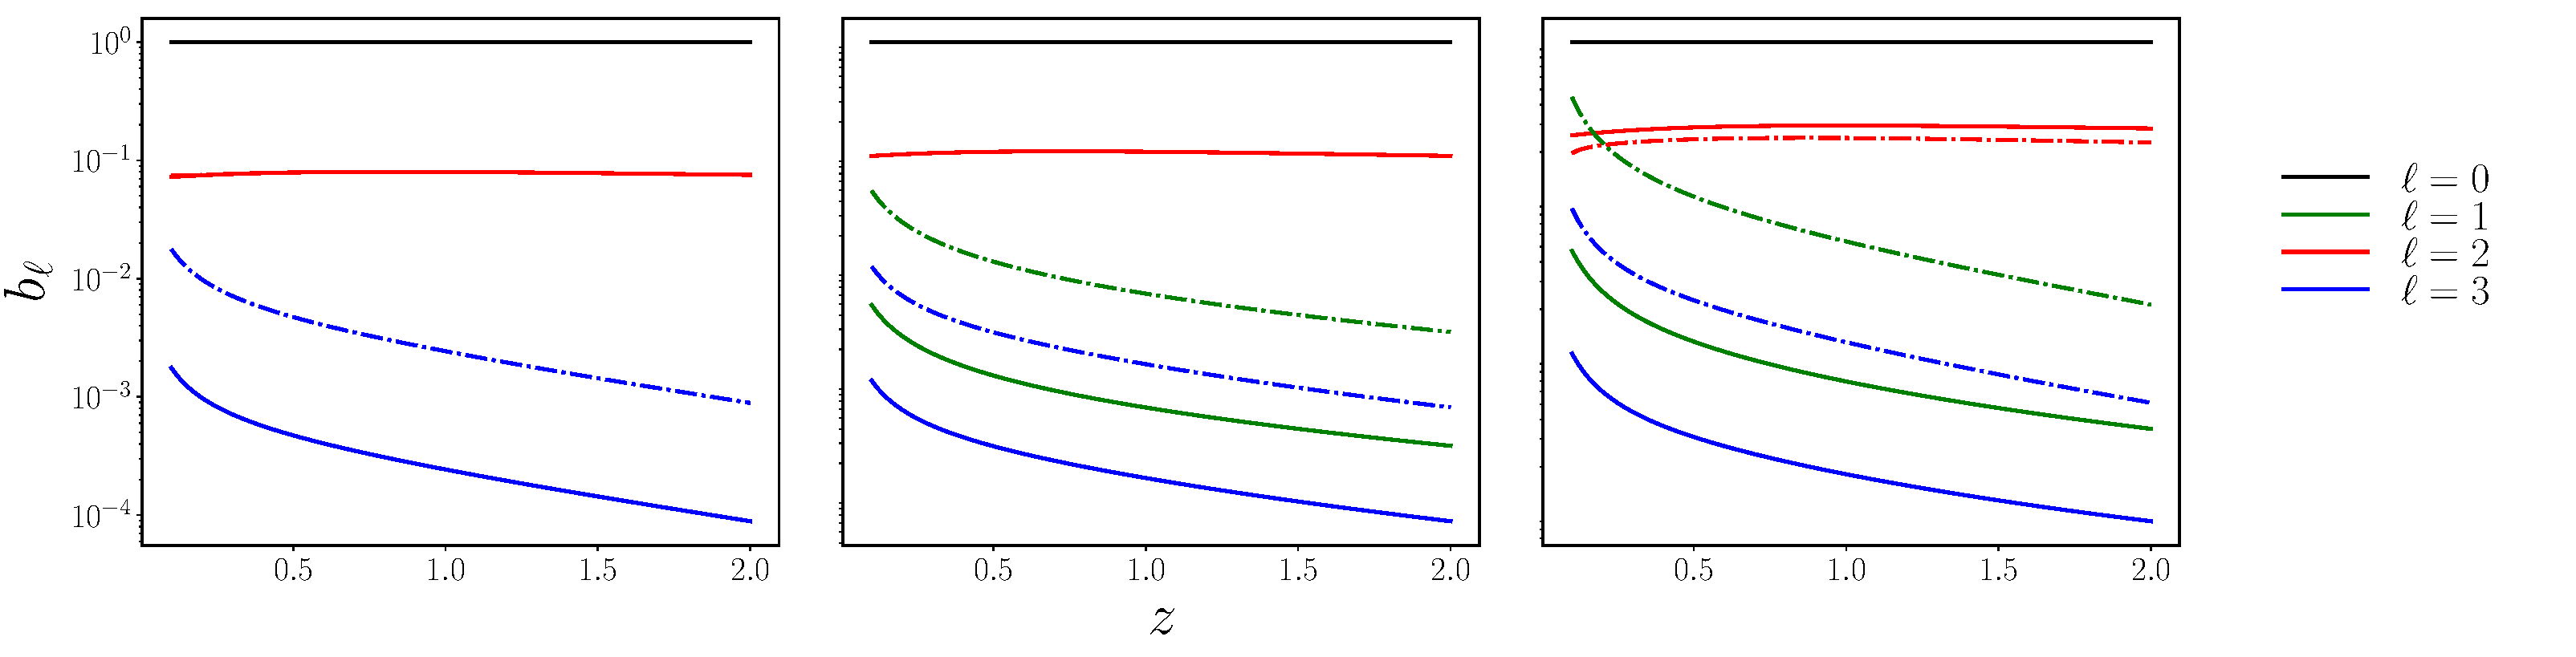
\includegraphics[width=\linewidth]{fig/fnofz.pdf}
\caption{Total power contained in the relativistic bispectrum normalised by the Newtonian monopole as a function of redshift \(z\) ranging from 0.1 to 2. The three panels are the equilateral configuration (left, with \(\ell = 1\) vanishing), squeezed (middle) and co-linear flattened configuration (right). Solid lines for \(k = 0.1 \, \mathrm{Mpc^{-1}}\), and dash-dotted for \(k = 0.01 \, \mathrm{Mpc^{-1}}\).\label{fig:fnofz}}
\end{figure}

Figures~\ref{fig:totpowersq},\ref{fig:totpowerfl} and~\ref{fig:totpowereq} show the amplitude of the total power as defined in~\eqref{eq:totpower}. For each $\ell$ this contains all orientations per multipole divided by the amplitude of the Newtonian monopole. Values of \(\ell\) are labelled on the figure, with the dotted lines denoting the Newtonian contribution (for even \(\ell\) only). For small scales (larger wavenumber \(k\)), the Newtonian contributions are generally larger than the relativistic \(b_\ell\) (i.e. odd \(\ell\)), however at larger scales,  above equality, the relative power contained in relativistic contributions increases. This shows up in the even multipoles as a divergence between the dotted (purely Newtonian) lines and solid (GR-corrected) lines. In the odd multipoles, we see an increase in amplitude, which at the largest scales become larger than the purely Newtonian signal. This is dependent on bias model and triangular configuration.

The colour-intensity maps in figures~\ref{fig:euclidtriangle} and~\ref{fig:imtriangle} show the amplitude of the relativistic bispectrum over the \(k_3/k_1\), \(k_2/k_1\) plane. The amplitude of the bispectrum signal peaks in the squeezed limit where \(k_1=k_2\), \(k_3\to 0\) which is in the top left corner in these plots. For the odd multipoles \(\ell = 1\) and \(\ell = 3\),  the amplitude of the dipole is higher than the \(\ell=3\) case in most configurations. The amplitude of the relativistic bispectrum is also higher for larger scales (smaller \(k\)). For \(\ell = 1\), the equilateral configuration, which lies in the upper right corner of the plots, is vanishing as we established analytically. 
We can also observe from these plots that there is a rough trend that more power is contained in the lower $m$ multipoles.

The reduced bispectrum is plotted in figure~\ref{fig:Q_rb}, showing large relativistic contributions to the bispectrum odd-multipoles especially at large scales. This also shows the significant dependence on the triangle shape, depending on the orientation of the harmonic.  

Finally figure~\ref{fig:fnofz} shows the total power divided by the Newtonian monopole, as a function of redshift. The model for bias used here is not physically realistic, but this illustrates the generic behaviour with redshift we can expect. It is interesting to observe how, when going towards lower redshift, the power in the relativistic corrections to the bispectrum grows compared to the Newtonian signal. This is especially noticeable in squeezed and flattened shapes where the dipole approaches or surpasses the \(\ell = 2\) line. Of course, at low redshift the plane-parallel assumption that we have used becomes a worse approximation.

\section{Conclusion}\label{sec:concl}
%
We have considered in detail for the first time the multipole decomposition of the observed relativistic galaxy bispectrum. In section~\ref{sec:extrmulti} we have shown how the multipoles may be derived analytically, with an analytic formula given in equation~\eqref{eq:sumformula}, and have illustrated how they behave in the squeezed, equilateral and co-linear limits (which includes the flattened case) in section~\ref{sec:anal}. We have shown how the amplitude of the relativistic signals behaves for two types of upcoming surveys~-- a Euclid-like galaxy survey, and an SKA intensity mapping survey. Our key findings are:
\begin{description}
\item[odd multipoles] Relativistic effects generate a hierarchy of odd multipoles which are absent in the Newtonian picture, plus an additional contribution to all multipoles up to $\ell=7$. In particular we find that the octopole is similar in amplitude to the dipole; it is only about a factor of 5 or so smaller than the dipole. These are both larger than the Newtonian hexadecapole on large scales. Higher multipoles are suppressed. This effect can be seen clearly in figures~\ref{fig:totpowersq},~\ref{fig:totpowerfl},~\ref{fig:totpowereq}.
%
\item[powers of $k$] The leading power of the relativistic correction in each $\ell$ harmonic is $(\cH/k)^1$ for odd multipoles and $(\cH/k)^2$, for even multipoles. Furthermore, all odd multipoles contain the leading $(\cH/k)$ correction, while lower values of \(\ell\) contain the higher powers of \(\cH/k\), going up to \((\cH/k)^7\) for \(\ell=1\) (though these are probably unobservable). An overview of occurring powers of \(k\) is given in figure~\ref{fig:blm_overview}.
%
\item[special limits] the co-linear case ($\theta=0$ or $\pi$) only generates non-zero $m=0$ multipoles and vanishes for all other values of \(m\). The equilateral case is always zero for $m$ odd, and is always zero for the special case of the dipole. For the squeezed limit we have leading $(\cH/k)$ relativistic corrections for $\ell$ and $m\leq3$ odd.
%
\item[multipoles with shape] We computed the amplitude of each $\ell,m$ over the range of triangle shapes in figures~\ref{fig:euclidtriangle},~\ref{fig:imtriangle}. For each $\ell$ most of the power is contained in the lower $m$ multipoles. 
%
\item[multipoles with scale] We analysed the total power in each multipole as a function of scale for 3 triangle shapes at $z=1$. Roughly speaking the even-$\ell$ are dominated by the Newtonian part and have little scale dependence relative to the Newtonian monopole, though this changes approaching the Hubble scale. For odd-$\ell$ the leading relativistic part dominates and the dipole reaches the size of the Newtonian quadrupole around equality scales.
%, while the octopole is only about a factor of 5 or so smaller than the dipole.
%
\item[redshift dependence] Relative to the Newtonian monopole, all the relativistic multipoles decay with redshift, while the quadrupole is roughly constant. For large squeezed triangles the dipole is comparable in size to the quadrupole for small redshift as shown in figure~\ref{fig:fnofz}.
%
\end{description}
Of course, the analysis here is limited by the fact we have neglected wide angle effects which will alter the multipoles.  Integrated effects will also contribute, but their effect will be suppressed when we analyse the multipoles. We leave these contributions for future work. Also currently under investigation is detectability of the galaxy bispectrum, with the leading order contribution examined in~\cite{Maartens:2019yhx}.

%
% !TEX root = ../thesis.tex

\chapter{Local primordial non-Gaussianity in the bispectrum}
\label{chapter:localpng}


Next-generation galaxy and 21cm intensity mapping surveys will rely on a combination of the power spectrum and bispectrum for high-precision measurements of primordial non-Gaussianity. In turn, these measurements will allow us to distinguish between various models of inflation. However, precision observations require theoretical precision at least at the same level. We extend the theoretical understanding of the galaxy bispectrum by incorporating a consistent general relativistic model of galaxy bias at second order, in the presence of local primordial non-Gaussianity. {The influence of primordial non-Gaussianity on the bispectrum extends beyond the  galaxy bias and the dark matter density, due to redshift-space effects. The standard redshift-space distortions at first and second order produce a well-known primordial non-Gaussian  imprint on the bispectrum. Relativistic corrections to redshift-space distortions
generate new contributions to this primordial non-Gaussian signal, arising from: (1)~a coupling of first-order scale-dependent bias with first-order relativistic observational effects, and (2)~linearly evolved non-Gaussianity in the second-order velocity and metric potentials which appear in relativistic observational effects.}
Our analysis allows for a consistent separation of the relativistic  `contamination' from the primordial signal, in order to avoid biasing the measurements by using an incorrect theoretical model. We show that the bias from using a Newtonian analysis of the squeezed bispectrum could be $\Delta \fnl\sim 5$ for a Stage IV H$\alpha$ survey. 

The content discussed in this chapter is taken from~\cite{Maartens:2020jzf}. The chapter is structured as follows. Section~\ref{ss-mvp} reviews the relativistic correction to the galaxy bias, including  the case of local PNG. In addition, we show how the linearly evolved second-order metric and velocity potentials carry a primordial non-Gaussian signal, which is imprinted in the bispectrum by relativistic projection effects. In Section~\ref{sec3}, after presenting the relativistic correction to the matter bispectrum, we discuss the number density contrast in redshift space, which brings into play the relativistic projection effects. We combine the various results to derive the relativistic galaxy bispectrum, including all local PNG effects, and we show examples of the galaxy bispectrum for a Stage IV H$\alpha$ spectroscopic survey. We summarise and conclude in Section~\ref{sec4}.

\section{Galaxy clustering statistics and primordial non-Gaussianity}

Galaxy number counts are distorted by projection effects that arise from observing on the past lightcone. {The dominant perturbative effect on sub-Hubble  scales is from redshift-space distortions (RSD) \cite{Sargent:1977,Kaiser:1987qv}, 
which constitute the standard Newtonian approximation to projection effects. Lensing magnification produces the best-known relativistic correction to RSD \cite{Villumsen:1995ar}, but there are further relativistic effects \cite{Yoo:2009au,Yoo:2010ni,Challinor:2011bk,Bonvin:2011bg}.
The basic idea is the following. The number of sources, $\ud \mathbb{N} $,  {above the luminosity threshold} that are counted by the observer in a solid angle element about unit direction $\n$ and in a redshift interval about a central redshift $z$, is given by 
\begin{equation} \label{dn}
\ud \mathbb{N} =N_g\, \ud z\,\ud\Omega_{\n}=  n_g\, \ud {\cal V} \,. 
\end{equation}
The second equality relates the observed quantities to those measured in the rest frame of the source.
$N_g$ is the number that is counted by the observer per redshift per solid angle, while 
$ n_g$ is the number per proper volume, which is not observed by the observer but is the quantity that would be measured at the source. Similarly,  $\ud {\cal V}$ is not the observed volume element but the corresponding proper volume element at the source.  

Then the observed number density contrast, $\Delta_g=(N_g-\bar{N}_g)/\bar{N}_g$, is related to the proper number density contrast at the source, $\delta_g=(n_g-\bar{n}_g)/\bar{n}_g$, by volume, redshift and {luminosity} perturbations. 
At first order  in Poisson gauge,  the gauge-independent relation \eqref{dn} leads to
\begin{align}
 \Delta_g&=\delta_g +\,\mbox{RSD +  lensing effect + other relativistic effects} \notag\\
\label{obdel}
&= \delta_g - \frac{1}{{\cal H}}\n \cdot \bm\nabla \big(\v  \cdot \n \big) + 2(1-{\cal Q})\kappa +  A\big(\v  \cdot \n \big)+B \Psi + \int\! \ud \chi\,C\Psi' +\int\! \ud \chi\,E\Psi \,.
\end{align}
Here ${\cal H}=\ud\ln a/\ud \eta=(\ln a)'$ is the conformal Hubble rate, $\v=\bm{\nabla} V$ is the peculiar velocity ($V$ is not to be confused with the often-used alternative $v=|\v|$), $\kappa$ is the integrated lensing convergence,  ${\cal Q}$ is the magnification bias, $\chi$ is the comoving line-of-sight distance and the integrals are from source to observer. 
The perturbed metric is given by
\begin{equation} \label{pds}
a^{-2}\ud s^2=-\big(1+2\Phi \big)\ud \eta^2+ \big(1-2\Psi \big)\ud \x^2\,,
\end{equation}
and we have assumed $\Phi=\Psi$. The time-dependent factors $A,B,C,E$ in \eqref{obdel} correspond respectively to Doppler, Sachs-Wolfe, integrated Sachs-Wolfe and time-delay effects. In Fourier space the Doppler term scales as $\partial V \propto ({\cal H}/k)\delta_m$, while the remaining terms scale as $\Psi \propto ({\cal H}/k)^2\delta_m$. Thus the other relativistic effects are suppressed on sub-Hubble scales, unlike the lensing effect, which scales as $\partial^2 \Psi \propto \delta_m$.

{The case of 21cm intensity mapping follows from the number count expressions  by using the `dictionary' given in \cite{Hall:2012wd,Alonso:2015uua,Fonseca:2015laa} at first order and in \cite{Umeh:2015gza,DiDio:2015bua,Jolicoeur:2020eup} at second order.}

The physical definition of linear Gaussian galaxy bias is in the joint matter-galaxy rest frame, which corresponds to the comoving gauge (`C gauge'),\footnote{In the $\Lambda$CDM model  the comoving and synchronous gauges coincide.} so that (omitting luminosity dependence for brevity), 
\begin{equation} \label{b1}
\delta_{g{\mathrm{C}}}(a,\x)=b_1(a)\delta_{m{\mathrm{C}}}(a,\x)\,.
\end{equation}
This relation is gauge-independent because C gauge corresponds to the physical rest frame.
When transforming to other gauges, $\delta_g$ is in general no longer proportional to $\delta_m$ \cite{Challinor:2011bk,Bruni:2011ta,Jeong:2011as}. For example,  in the Poisson gauge of  \eqref{obdel} and~\eqref{pds}, 
\begin{equation} \label{b1pg}
\delta_g =b_1\delta_{m{\mathrm{C}}} + (3-b_e){\cal H}V\,,\quad b_e = \frac{\partial \ln (a^3\bar{n}_g)}{\partial \ln a}\,,
\end{equation}
where $b_e$ is known as the evolution bias, which encodes the non-conservation of the background comoving galaxy number density. The velocity potential $V$ scales as $\Psi$ by the {Euler} equation, $ V\propto  \Psi \propto ({\cal H}/k)^2\delta_m$, and therefore
the gauge correction $(3-b_e){\cal H}V$ is only non-negligible on Hubble scales and may be neglected in a Newtonian approximation. 

Local  primordial non-Gaussianity (PNG) generates scale-dependent linear bias, with constant parameter $\fnl$ 
\cite{Dalal:2007cu,Matarrese:2008nc}:
\begin{equation} \label{b1ng}
 b_{1}(a)~\to~ b_1(a)+3\,\delta_{\mathrm{crit}}\Omega_{m0}H_0^2 \, \frac{\big[b_1(a)-1 \big]}{D(a)}\, 
 g_{\in}\, \frac{\fnl}{T(k)k^2}\,.
\end{equation}
The threshold density contrast for collapse is usually taken to be $\delta_{\mathrm{crit}}=1.686$, and the growth factor $D$  is normalised to 1 today ($a_0=1$), i.e. $\delta_m(a,\k)=D(a)\delta_{m0}(\k) $. The growth suppression factor for the potential $\Psi$ is $g=D/a$, which is thus also normalised as $g_0=1$, with initial value $g_{\in}$ deep in the matter era,  and $T$ is the  transfer function. Note that \eqref{b1ng} follows the CMB convention
%\footnote{In this convention, the $g_{\in}$ factor can be removed if $D$ is normalised as $D_{\in}=a_{\in}$; see e.g.  \cite{Desjacques:2016bnm}.} 
for $\fnl$ \cite{Baldauf:2010vn,Desjacques:2016bnm};  $g_{\in}$ can be removed from \eqref{b1ng} if $D$ is normalised as $D_{\in}=a_{\in}$.  
In a $\Lambda$CDM model we have the useful relation \cite{Villa:2015ppa}
\begin{equation} \label{ggin}
\frac{g_{\in}}{g}= \frac{3}{5}\Big(1+ \frac{2f}{3\Omega_m} \Big),
\end{equation}
where the growth rate of linear matter perturbations, $f=\ud \ln D/\ud \ln a$, is very well approximated by $f(a)=\Omega_m(a)^{0.545}$. 

The PNG component of galaxy bias in \eqref{b1ng} 
scales as $H_0^2/k^2$ on ultra-large scales, i.e. above the equality scale, $k< k_{\mathrm{eq}}$, where $T\approx 1$. It
is strongly suppressed on scales $k\gg k_{\mathrm{eq}}$ by $T(k)$. PNG has a similar impact on the power spectrum to the impact of ultra-large-scale relativistic effects. This means that relativistic effects contaminate the primordial signal --  leading to  biases if a Newtonian approximation is used to model the galaxy power spectrum (see \cite{Bruni:2011ta, Jeong:2011as, Camera:2014sba}). 
The relativistic galaxy power spectrum has been used to analyse and predict the capability of future galaxy and intensity mapping surveys to
measure the local PNG parameter $\fnl$, while avoiding the bias  that is inherent in a Newtonian analysis (see e.g. \cite{Bruni:2011ta, Jeong:2011as, LopezHonorez:2011cy, Yoo:2012se, Raccanelli:2013dza,Camera:2014bwa, Camera:2014sba, Raccanelli:2015vla, Alonso:2015uua, Alonso:2015sfa, Fonseca:2015laa, Fonseca:2016xvi, Abramo:2017xnp, Lorenz:2017iez, Fonseca:2018hsu, Ballardini:2019wxj, Grimm:2020ays, Bernal:2020pwq, Wang:2020ibf}).  

The tree-level bispectrum requires the number counts
in redshift space up to second order.
In the Newtonian approximation, the projection effects are the second-order RSD terms (see e.g. \cite{Tellarini:2016sgp}). The relativistic corrections
 to RSD at second-order  are extremely complicated, since they involve quadratic couplings of all the first-order terms, as well as introducing new terms that do not enter at first order, such as the {transverse peculiar velocity}, the lensing deflection angle and the lensing shear  \cite{Bertacca:2014dra, Bertacca:2014wga, Yoo:2014sfa, DiDio:2014lka, Bertacca:2014hwa}.   {There are further relativistic corrections that are not projection effects. Firstly,
 the Newtonian model of second-order galaxy bias in the comoving frame requires a relativistic correction, unlike the first-order bias (see Section~\ref{sdb}). Secondly,
 and similar to the first-order case, the second-order galaxy bias relation needs  relativistic gauge corrections  when using non-comoving gauges such as the Poisson gauge. These are second-order extensions of equations like \eqref{b1pg}.}  
{In summary, the second-order relativistic corrections to the galaxy bispectrum in the Gaussian case are: 
\begin{itemize}
\item
relativistic projection corrections to the Newtonian RSD  \cite{Bertacca:2014dra, Bertacca:2014wga, Yoo:2014sfa, DiDio:2014lka, Bertacca:2014hwa};
\item
relativistic corrections to the Newtonian bias model in the comoving frame at second order, which were only recently derived  \cite{Umeh:2019qyd, Umeh:2019jqg};
\item  
 relativistic gauge corrections to the second-order number density when using non-comoving gauges   \cite{Bertacca:2014dra, Bertacca:2014wga}. 
 \end{itemize}}

As in the case of the power spectrum, local PNG affects the bispectrum on very large scales, which is also where the relativistic effects are strongest. This leads again to a contamination of the primordial signal by relativistic effects, necessitating a relativistic analysis. A Gaussian primordial universe could be mistakenly interpreted as non-Gaussian if a Newtonian model is used for the bispectrum in analysis of the data, as shown by 
\cite{Kehagias:2015tda,Umeh:2016nuh,Jolicoeur:2017nyt,Koyama:2018ttg}. 

{There are important differences between the power spectrum and bispectrum:
\begin{itemize}
%\item
%The relativistic signal in the tree-level  bispectrum can reach smaller scales than in the tree-level power spectrum, because of the coupling of ultra-long to short modes in the 3-point correlations. 
\item
At first order, there is no relativistic correction to the bias model in comoving gauge -- the relativistic correction arises at second order \cite{Umeh:2019qyd, Umeh:2019jqg}. Therefore the tree-level bispectrum contains a relativistic correction to the bias model, but the tree-level power spectrum does not.
\item
There is no PNG signal in the primordial {\em matter} power spectrum at tree level, so that the local PNG signal in the tree-level galaxy power spectrum is sourced only by scale-dependent bias. 
\item
By contrast, local PNG in the galaxy bispectrum is sourced by scale-dependent bias, by the primordial matter bispectrum {and by RSD at second order (see \cite{Tellarini:2016sgp} and Section \ref{ss-mvp} below)}.
\item
 Second-order relativistic {corrections to RSD}  induce new local PNG effects in the bispectrum, via~(1) a coupling of first-order scale-dependent bias to first-order relativistic projection effects,  and {(2)~the linearly evolved PNG in second-order velocity and metric potentials, which appear in relativistic projection effects (absent in the standard Newtonian analysis)}. 
\end{itemize}}

Since local PNG affects the power spectrum and bispectrum differently, a Newtonian analysis could mistakenly identify inconsistencies between the power spectrum and bispectrum $\fnl$ measurements, which could wrongly lead to an inference of hidden systematics or deviations from general relativity.}

PNG in the galaxy bispectrum has been extensively investigated in the Newtonian approximation. Most work has used the Fourier bispectrum, implicitly incorporating a plane-parallel assumption (see e.g. 
\cite{Verde:1999ij,Scoccimarro:2003wn,Sefusatti:2006pa,Sefusatti:2007ih,Giannantonio:2009,Baldauf:2010vn,Tellarini:2015faa,Tellarini:2016sgp,Desjacques:2016bnm,Watkinson:2017zbs,Majumdar:2017tdm,Karagiannis:2018jdt,Yankelevich:2018uaz,Sarkar:2019ojl,Karagiannis:2019jjx,Bharadwaj:2020wkc,Karagiannis:2020dpq, MoradinezhadDizgah:2020whw}) and we follow this approximation.
Our previous work~\cite{Umeh:2016nuh} included the local (non-integrated) relativistic effects in the Fourier bispectrum for the first time. This was extended by our work~\cite{Jolicoeur:2017nyt, Jolicoeur:2017eyi, Jolicoeur:2018blf,Clarkson:2018dwn,Maartens:2019yhx,deWeerd:2019cae, Jolicoeur:2020eup, Umeh:2020cag}, all in the case of primordial Gaussianity. 
Here we incorporate local PNG into the relativistic bispectrum. This involves applying the recent results of~\cite{Umeh:2019qyd, Umeh:2019jqg} on relativistic corrections to the second-order galaxy bias model. {In addition, we derive the new local  PNG terms induced by  a coupling of first-order scale-dependent bias and first-order relativistic projection effects and by linearly evolved second-order relativistic projection effects.}
%
%\newpage
~\\ \noindent {\textbf{\em Conventions used:}} 
%
We assume  a flat $\Lambda$CDM model, based on general relativity and perturbed up to second order, in which the matter is pressure-free and irrotational on perturbative scales. Generalisations to allow dynamical dark energy and relativistic modified gravity are straightforward, but are not included. For numerical calculations, we use the Planck 2018 best-fit parameters \cite{Aghanim:2018eyx}.
Perturbed quantities are expanded as
$X+X^{\tw}/2$, and may be split as  $X_{\mathrm{N}}+X_{\mathrm{GR}}+X_{\mathrm{nG}}$, 
and similarly at second order, where N denotes the Newtonian approximation, GR denotes the relativistic correction and  nG denotes the local PNG contribution. {GR corrections are highlighted in \blue{magenta}.}
%
Our definition of the metric potentials in \eqref{pds} leads to the first-order Poisson equation 
\begin{equation} \label{pe1}
\nabla^2 \Psi= + \frac{3}{2}\Omega_m{\cal H}^2\,\delta_{\mathrm{C}} \,,
\end{equation}
where  $ \Phi= \Psi$ in $\Lambda$CDM. Here and in the remainder of the paper, we omit the subscript $m$ on the matter density contrast for brevity.
At second order, the perturbed metric in Poisson gauge is given by
\begin{equation} \label{pds2}
a^{-2}\ud s^2=-\big[1+2\Psi + \Phi^{\tw}\big]\ud \eta^2+ \big[1-2\Psi -  \Psi^{\tw}\big]\ud \x^2\,.
\end{equation}
\bro{Here we have neglected the relativistic vector and tensor modes that are generated by scalar mode coupling, so that we only consider the relativistic scalar contribution to the bispectrum. This approximation is justified by the fact that the relativistic vector contribution to the bispectrum is typically 2 orders of magnitude below the relativistic scalar contribution on observable scales, while the relativistic tensor contribution is typically an order of magnitude below that of the vector contribution (see \cite{Jolicoeur:2018blf}).}
%
%The comoving curvature perturbation ${\cal R}$ generated in the primordial inflationary era,  is gauge invariant and constant in time on super-Hubble scales.  On these scales, it is related to the primordial potential as ${\cal R}^{\on}(\x)=5 \Psi^{\on}_{\rm p}(\x)/3$.
%following \citep{Villa:2015ppa}, with $\Phi$ and $\Psi$ interchanged.
%--------------------------------------------------------------------------
%
%
\section{Local primordial non-Gaussianity in the galaxy bias}
\label{sdb}
%
Local PNG is defined as a simple form of nonlinearity in the primordial curvature perturbation, which is local in configuration space. In terms of the gravitational potential {deep in the matter era}, we have
%\footnote{{We have omitted an additional non-local term: see \cite{Umeh:2019jqg} for details.}} 
\begin{equation}
-\Big[\Psi_{\in}(\x) + \frac{1}{2} \Psi^{\tw}_{\in}(\x)\Big] = \varphi_{\in}(\x) + \fnl\big[\varphi_{\in}(\x)^{2}  - \big\langle \varphi_{\in}^{2} \big\rangle\big],
%\tilde{f}_{\rm NL}\,\nabla^{-2} \big(\partial_i\varphi_{\rm p} \partial^i\varphi_{\rm p}\big)  - \big\langle \mbox{2nd order terms} \big\rangle .}
\label{e1.1} 
\end{equation}
where $\varphi_{\in}$ is the first-order Gaussian part.
The standard definition of $\fnl$ uses a convention for $\Psi$ that is different to ours, with a minus on the right of the Poisson equation \eqref{pe1}. In order to keep the standard sign of $\fnl$, we made a sign change on the left of \eqref{e1.1}.
($\fnl$  in  \cite{Villa:2015ppa,Koyama:2018ttg, Umeh:2019jqg} is  of opposite sign to the standard sign that we use.) 
%
\subsection{First-order bias}
%
In~\eqref{e1.1}, the Gaussian part of the potential deep in the matter era {(but after decoupling)} is {related to the linear primordial potential by the transfer function:
\begin{equation} \label{vpe}
\varphi_{\in}(\k)=T(k)\,\varphi_{\mathrm{p}}(\k) {\quad \mbox{for}\quad a_{\mathrm{p}}\ll a_{\mathrm{eq}} \ll a_{\in} \,. }
\end{equation}
{Here $\varphi_{\mathrm{p}}(\k)=-9
\Psi(a_{\mathrm{p}},\k)/10$, where  the factor 9/10 ensures conservation of the curvature perturbation on super-Hubble scales.}
After equality, the potential evolves with the growth suppression factor, so that
\begin{equation}\label{pottp}
{\varphi(a,\k) = \frac{g(a)}{g_{\in}}  \varphi_{\in}(\k) \quad \mbox{for}\quad a\geq a_{\in}> {a_{\mathrm{dec}}}\,.}
\end{equation}
\begin{figure}[!ht]
\centering
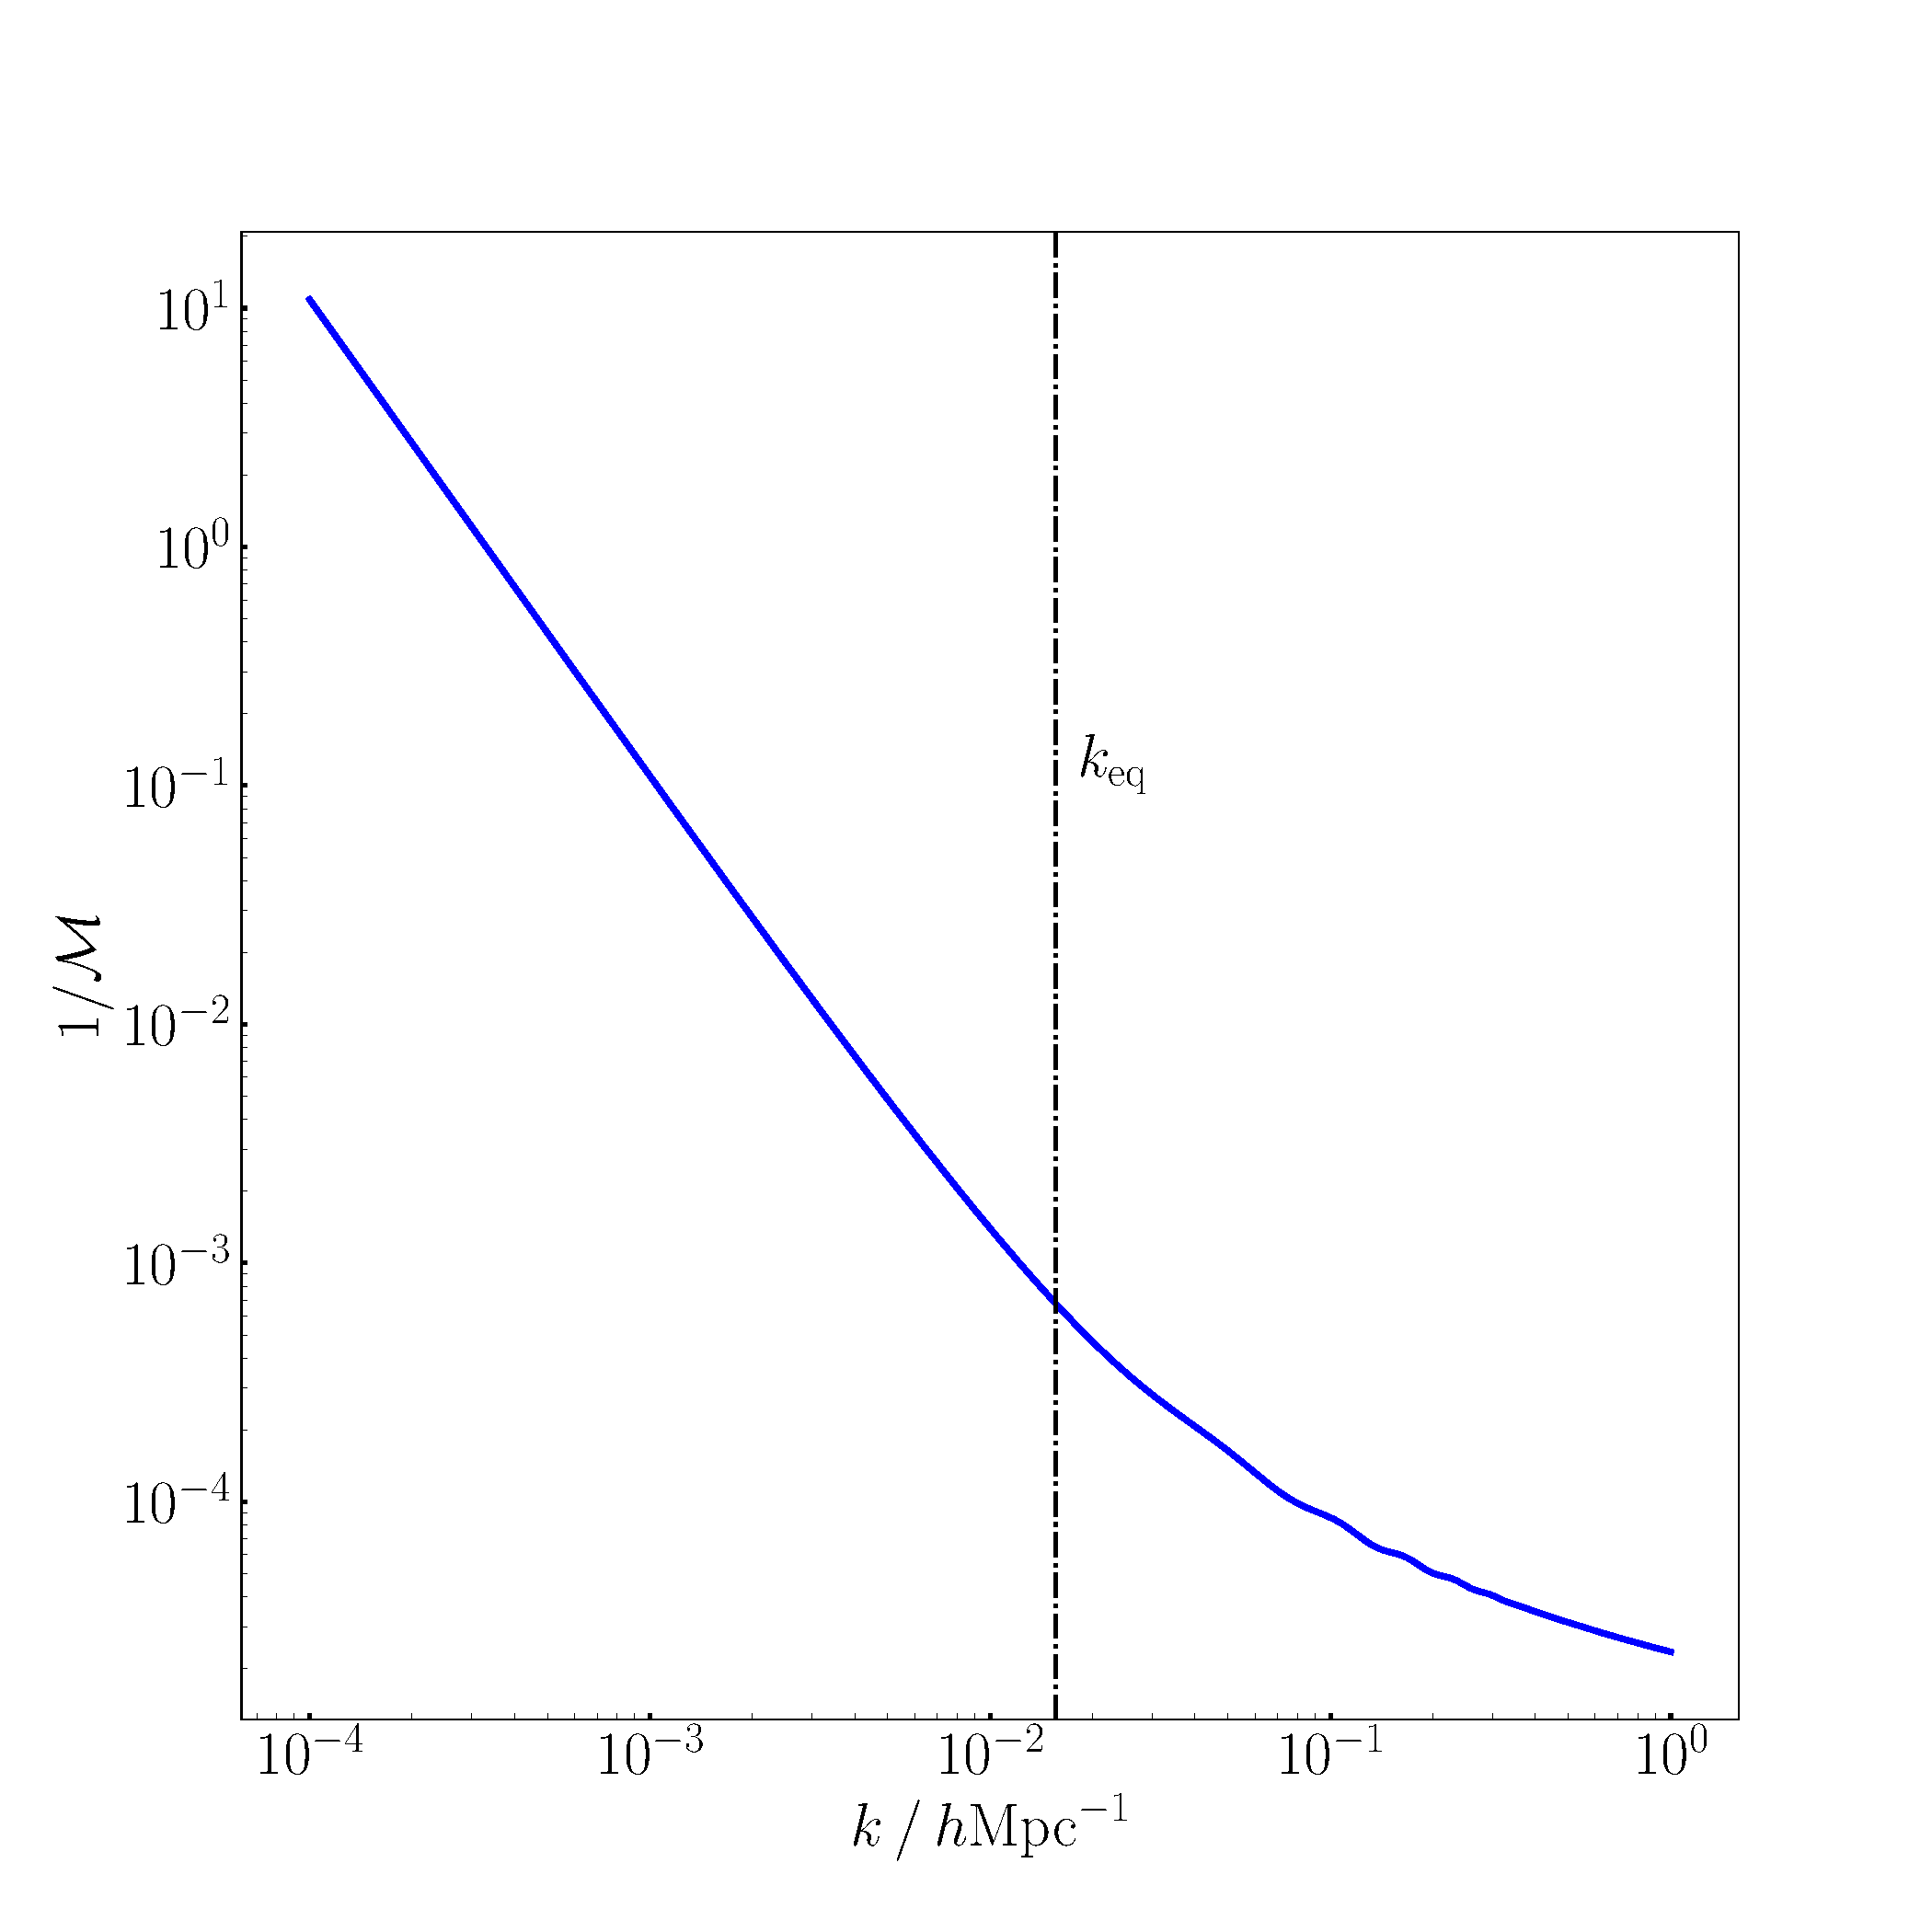
\includegraphics[width=.8\textwidth]{fig/Mplot.pdf}
\caption{{${\cal M}^{-1}= \varphi_{\mathrm{p}}/\delta^{\on}_{\mathrm{C}}$ at $z=1$.}}
\label{mplot}
\end{figure}

We relate the late-time matter density contrast  to the primordial potential via the Poisson equation \eqref{pe1}, using \eqref{ggin}, \eqref{vpe} and \eqref{pottp}:
\begin{align} \label{alpha}
\delta_{\mathrm{C}}(a,\k)=  {\cal M} (a,k)  \varphi_{\mathrm{p}} (\k) \quad \mbox{where} \quad 
{{\cal M} (a,k)  = \frac{10}{3\cH(a)^2\big[3\Omega_m(a) +2f(a) \big]}\,k^2 \, T(k)}\,.
% = {2 \over 3\Omega_{m0} H_0^2 }\,{D(a)\over g_{\in}}\,T(k)\,k^2\,.
\end{align}
This relation is illustrated in Figure~\ref{mplot}. 
{The matter and number density contrasts can be written as 
\begin{equation} \label{dcng}
\delta_{\mathrm{C}}= \delta_{\mathrm{C,N}} \quad \mbox{and}\quad
\delta_{g\mathrm{C}}= \delta_{g\mathrm{C,N}}+ \delta_{g\mathrm{C,nG}} \,.
\end{equation}
This follows since there is no GR correction to either contrast and no PNG in the Gaussian matter density contrast:}
\begin{equation} \label{dgro1}
\blue{\delta_{{\mathrm{C,GR}}} = 0 =\delta_{g{\mathrm{C,GR}}}}\,,\quad \delta_{{\mathrm{C,nG}}} =0\,.
%\qquad \delta_{g{\rm C}}=\delta_{g{\rm C,N}}=\delta_{g{\rm C,GR}}\,.
\end{equation}
Then it follows that}
\begin{equation}\label{dg1b}
\delta_{g{\mathrm{C}}}= \delta_{g \mathrm{C,N}}+ \delta_{g{\mathrm{C,nG}}}=   b_{10}\,\delta_{\mathrm{C}}+ b_{01}\,\varphi_{\mathrm{p}}\,, 
\end{equation}
where the Gaussian and non-Gaussian  bias coefficients are 
\begin{equation}
\label{bias1}
b_{10}= b_1\,,\quad
b_{01}= 2\fnl \delta_{\mathrm{crit}}(b_{10}-1)\,.
\end{equation}
The relations \eqref{alpha}--\eqref{bias1} then recover \eqref{b1ng}.

{At first order,  there is {\em no} GR correction to the  bias relation  expressed in the matter-galaxy rest frame. This is no longer true at second order.

The first-order metric  potential is Gaussian by \eqref{e1.1} and has no GR correction by \eqref{dgro1} and  the Poisson equation. From the Euler equation ($V'+{\cal H}V=- \Psi$) it follows that the velocity also has no GR and no PNG corrections:
\begin{equation} \label{pvo1}
\Psi=\Psi_{\mathrm{N}}\,,\qquad V=V_{\mathrm{N}}\,.
\end{equation}
%
\subsection{Second-order bias: {Newtonian} approximation}
%
At second order, the  galaxy bias is {physically} defined in comoving gauge, {but any gauge may be used in general relativity. Standard Newtonian perturbation theory is often given in an Eulerian frame, and so it is useful for comparison}  to express the  bias in a suitable Eulerian frame. We use Poisson gauge here, following~\cite{Umeh:2016nuh,Tram:2016cpy, Jolicoeur:2017nyt, Jolicoeur:2017eyi, Jolicoeur:2018blf,Clarkson:2018dwn,Maartens:2019yhx,deWeerd:2019cae}, but with the galaxy and matter density contrasts in total-matter gauge (`T gauge').}  {The total-matter gauge is a convenient  Eulerian choice  for the density contrasts, since it has the same spatial coordinates as the Poisson gauge at first order and the same time-slicing as the comoving gauge at first and second orders~\cite{Bartolo:2015qva,Villa:2015ppa,Tram:2016cpy}. 
As a result, at first order
the total-matter density contrasts coincide with those of the comoving gauge: 
$\delta_{{\mathrm{T}}}=\delta_{{\mathrm{C}}}$, $\delta_{g{\mathrm{T}}}=\delta_{g{\mathrm{C}}}$, 
and we can rewrite  \eqref{dg1b} as 
\begin{align}
\delta_{g{\mathrm{T}}} &={\delta_{g \mathrm{T,N}} + \delta_{g{\mathrm{T,nG}}}} \\
&=b_{10}\,\delta_{\mathrm{T}}+ b_{01}\,\varphi_{\mathrm{p}}={\Big(b_{10} + \frac{b_{01}}{{\cal M}} \Big) \delta_{\mathrm{T}}}\,.
 \label{dg1bt}
\end{align}

 
At second order, the total-matter and Poisson matter density contrasts agree in the Newtonian approximation: 
$\delta_{\mathrm{T,N}}^{\tw}=\delta^{\tw}_{\mathrm{N}}$, while the comoving and total-matter Newtonian density contrasts are related via a purely spatial gauge transformation \cite{Bertacca:2015mca,Villa:2015ppa, Jolicoeur:2017nyt,Umeh:2019qyd}: 
\begin{equation} \label{ttc2}
{\delta_{\mathrm{T,N}}^{\tw}} = {\delta_{\mathrm{C,N}}^{\tw}}+2\xi^i\partial_i \delta_{{\mathrm{C}}} \,,\quad {\delta_{g\mathrm{T,N}}^{\tw}} = {\delta_{g\mathrm{C,N}}^{\tw}}+2\xi^i\partial_i \delta_{{g\mathrm{C}}} \,, 
\end{equation}
where
\begin{equation} \label{xi}
\xi^i = \partial^i \nabla^{-2}\delta_{{\mathrm{C}}} = \partial^i \nabla^{-2}\delta_{{\mathrm{T}}} \,.
\end{equation}
(The GR parts of the second-order density contrasts in comoving and total-matter gauges are equal; see below.)

{For the small scales involved in local clustering of matter density, the Poisson equation at second order has the same Newtonian form as at first order.
%\footnote{Relativistic corrections to the Poisson equation \cite{Bruni:2013qta,Bartolo:2015qva,Umeh:2019jqg} are related to the relativistic corrections that we describe in the following.}
 {Then we can extend~\eqref{alpha} up to second order to define the linearly evolved local PNG part of the density contrast, whose nonlinearity is purely primordial: 
\begin{equation} \label{alpha1a}
\delta_{\mathrm{T,nG}}^{\tw}={\cal M} \,\varphi_{\mathrm{p}}^{(2)} = 2\fnl  \,{\cal M} \,\varphi_{\mathrm{p}}*\varphi_{\mathrm{p}}\,,
\end{equation}
where the $*$ denotes a convolution in Fourier space.
%Thus 
%\be \label{alpha1a}
%\delta_{\rm T}+ {1\over 2}\,{\delta_{\rm T,nG}^{\tw}} = {\cal M}\big( \varphi_{\rm p} +\fnl \,\varphi_{\rm p}*\varphi_{\rm p}\big),
%\ee
This leads to
\begin{equation} \label{alpha2}
\delta_{\mathrm{T,nG}}^{\tw}= 2\fnl \,{\cal M} (a,k)\int \frac{\ud \k'}{(2\pi)^3}\, \frac{\delta_{\mathrm{T}}(a,\k')}{{\cal M} (a,k')}\, \frac{\delta_{\mathrm{T}}(a,\k-\k')}{{\cal M} (a,|\k-\k'|)}\,.
\end{equation}

In order to include the nonlinearity due to gravitational evolution, we add the standard Newtonian  contribution for Gaussian initial conditions to the local PNG part:}  
\begin{align} \label{alpha3}
%\delta_{\rm T,N}^{\tw}(a,\k)&=& 
&\delta_{\mathrm{T,{N}}}^{\tw}(a,\k) + \delta_{\mathrm{T,nG}}^{\tw}(a,\k)  
\\ \notag 
&{}= \int \frac{\ud \k'}{(2\pi)^3}\, \bigg[{F_{2}}(a,\k',\k-\k') +  2\fnl \,\frac{{\cal M} (a,k)}{{\cal M} (a,k')\, {\cal M} (a,|\k-\k'|)} \bigg] \delta_{\mathrm{T}}(a,\k')\,\delta_{\mathrm{T}}(a,\k-\k') \,.
\end{align}
The standard Newtonian mode-coupling kernel
%\footnote{Our perturbative convention leads to an $F_2$ that is twice the $F_2$ in the alternative convention.} 
for $\Lambda$CDM is~\cite{Villa:2015ppa}:
\begin{equation}
F_{2}(a,\bm{k}_{1},\bm{k}_{2}) = 1 + \frac{F(a)}{D(a)^2} + \Big(\frac{k_1}{k_2}+ \frac{k_2}{k_1}\Big)\hat{\k}_1\cdot \hat{\k}_2 +\bigg[1 - \frac{F(a)}{D(a)^2}\bigg]\big( \hat{\k}_1\cdot \hat{\k}_2\big)^2\,,\label{f2k}
\end{equation}
where $F$ is the second-order growth factor.  The Einstein--de Sitter relation $F/D^2=3/7$ is a very good approximation in $\Lambda$CDM. We use this approximation, in which $F_2$ is effectively time independent.}

At second order, the standard Newtonian bias model, including tidal bias in the Gaussian part and all local PNG contributions, is given by (see~\cite{Desjacques:2016bnm} for a comprehensive treatment):
\begin{align}
\delta^{\tw}_{g{\mathrm{T,{N}}}} +\delta_{g\mathrm{T,nG}}^{\tw} &= b_{10}\, {\delta^{\tw}_{{\mathrm{T,{N}}}}}+ b_{20} \big(\delta_{{\mathrm{T}}}\big)^2   + b_s\,s^2 
\notag \\
& +b_{10}\, \delta_{\mathrm{T,nG}}^{\tw} + b_{11}\, \delta_{{\mathrm{T}}}\,\varphi_{\mathrm{p}} +  b_{{n}}\, \xi^i\,\partial_i\,\varphi_{\mathrm{p}}+b_{02} \big(\varphi_{\mathrm{p}}\big)^2\,. \label{dg2bn}
\end{align}
The (Eulerian) bias parameters in the case of Gaussian initial conditions are in the first line on the right-hand side:  the  linear and quadratic biases, $b_{10}$ and $b_{20}$, and the tidal bias $b_s$, where  
\begin{equation} \label{ts}
s^2=s_{ij}s^{ij}\,, \quad s_{ij} =\Big(\partial_i \partial_j - \frac{1}{3}\delta_{ij}\nabla^2 \Big){\nabla^{-2}\delta_{\mathrm{T}}} 
\,.
\end{equation}
The second line of~\eqref{dg2bn} contains the local PNG contribution, with three new bias parameters $b_{11}, b_{{n}}, b_{02}$. The first term is the {primordial dark matter contribution}, from~\eqref{alpha3}; note that $\tilde\delta^{\tw}_{{\mathrm{T,N}}}$ is proportional to $\fnl$.
{The $b_{11}, b_n$ terms scale as $(\cH^2/k^2)\,(\delta_{\mathrm{T}})^2$, while the $b_{02}$ term is $\mathcal{O}(\cH^4/k^4)$.}
 The new bias parameters vanish when $\fnl=0$; in the presence of local PNG, they are given by~\cite{Tellarini:2015faa, Desjacques:2016bnm,Umeh:2019jqg}: 
\begin{align}
b_{11} &= 4\fnl \Big[\delta_{\mathrm{crit}}\,b_{20}+\Big(\frac{13}{21}\delta_{\mathrm{crit}}-1 \Big) (b_{10}-1)+1\Big] 
\,, \label{b11}
\\
b_{{n}} &= 4\fnl \Big[ \delta_{\mathrm{crit}}(1-b_{10}) +1\Big] \,,  \label{bxi}
\\
b_{02} &= 4\fnl^2 \delta_{\mathrm{crit}}\Big[\delta_{\mathrm{crit}}\,b_{20}-2\Big( \frac{4}{21}\delta_{\mathrm{crit}}+1 \Big) (b_{10}-1)\Big]. \label{b02}
\end{align}
Note that the expressions for the bias coefficients in~\eqref{b11}--\eqref{b02}, as well as for $b_{01}$ in~\eqref{bias1}, are based on a universal halo mass function. {(For recent work on the limits of the universality assumption, see~\cite{Barreira:2020kvh,Barreira:2020ekm}.)} 
%
\subsection{Second-order bias: {relativistic corrections}}
%
{The relativistic second-order galaxy bias model has been derived in~\cite{Umeh:2019qyd} (Gaussian case) and~\cite{Umeh:2019jqg} (with local PNG). {The key feature to bear in mind is the following:
 \begin{quote} 
{\em GR corrections in the galaxy number density contrast $\delta^{\tw}_{g{\mathrm{T}}}$ do not change the galaxy bias terms in \eqref{dg2bn}, which contain all the local PNG effects.}
\end{quote}
This separation between GR effects and local PNG in the number density can be understood as follows. 
\begin{itemize}
\item
The intrinsic  nonlinearity of GR  modulates the galaxy number density  via large-scale modes. 
However,  this does not affect small-scale clustering: GR effects do {\em not} modulate the variance of small-scale density modes~\cite{Koyama:2018ttg,Dai:2015jaa,dePutter:2015vga}.
\item
By contrast, local PNG imprints a primordial long-short coupling that induces a long-mode modulation of the variance and thus changes the galaxy bias.
\end{itemize}
As a consequence, we expect that relativistic corrections to the bias relation should be independent of  non-Gaussianity and apply only on ultra-large scales  (for a different view, see~\cite{Matarrese:2020why}). 
These two features are consistent with the behaviour of~\eqref{dg2bn} under change of gauge:
 \begin{quote} 
{\em The Newtonian bias relation~\eqref{dg2bn} is gauge-independent only on small scales.\\
Relativistic
corrections to~\eqref{dg2bn}  are needed to enforce gauge-independence of the bias relation on ultra-large scales.}
\end{quote}

As shown in~\cite{Umeh:2019qyd,Umeh:2019jqg}, gauge-independence requires the addition to~\eqref{dg2bn} of the relativistic part of the second-order matter density contrast. The relativistic modes are super-Hubble at equality and arise from nonlinear GR corrections to the Newtonian Poisson equation~\cite{Bruni:2013qta,Bartolo:2015qva,Villa:2015ppa,Tram:2016cpy}: 
\begin{align} \label{dtgr2}
\blue{\delta_{\mathrm{C,GR}}^{\tw}=\delta_{\mathrm{T,GR}}^{\tw} =
\frac{20}{3}\, \delta_{{\mathrm{T}}}\,{\hat{\varphi}_{\mathrm{in}}} 
- \frac{5}{3}\, \xi^i\,\partial_i \, {\hat\varphi_{\mathrm{in}}} \equiv \delta^{\tw}_{g{\mathrm{T,GR}}}}\,. 
\end{align}
Here $\hat\varphi_{\mathrm{in}}$ is the ultra-large scale potential deep in the matter era, 
\begin{equation} \label{hatv}
 \hat\varphi_{\mathrm{in}}(\k) =  \varphi_{\mathrm{in}}\big(\k\, | \, k<k_{\mathrm{eq}}\big) \,.
\end{equation}
When we relate $\hat\varphi_{\mathrm{in}}$ to the density contrast today, via \eqref{vpe} and \eqref{alpha}, we need to impose $T=1$ on the transfer function, by \eqref{hatv}.}

The relativistic second-order galaxy bias model of~\cite{Umeh:2019jqg} can  be written in T-gauge as
\begin{equation}
\delta^{\tw}_{g{\mathrm{T}}} = \delta^{\tw}_{g{\mathrm{T,N}}}+ \delta_{g\mathrm{T,nG}}^{\tw} +\blue{\delta^{\tw}_{g{\mathrm{T,GR}}}}
\,,
\label{dg2b1}
\end{equation}
where
\begin{align}
\delta^{\tw}_{g{\mathrm{T,N}}} &= b_{10}\, \delta^{\tw}_{{\mathrm{T,N}}}+ b_{20} \big(\delta_{{\mathrm{T}}}\big)^2   + b_s\,s^2 \,,
\label{dg2b2}\\
\delta_{g\mathrm{T,nG}}^{\tw} &= b_{10}\,  \delta_{\mathrm{T,nG}}^{\tw}
 + b_{11}\, \delta_{{\mathrm{T}}}\,\varphi_{\mathrm{p}} +  b_{{n}}\, \xi^i\,\partial_i\,\varphi_{\mathrm{p}}+b_{02} \big(\varphi_{\mathrm{p}}\big)^2,
\label{dg2b3} \\
\blue{\delta^{\tw}_{g{\mathrm{T,GR}}}}&\blue{=} \blue{\frac{20}{3}\, \delta_{{\mathrm{T}}}\,\hat\varphi_{{\mathrm{in}}} - \frac{5}{3}\, \xi^i\,\partial_i\,\hat\varphi_{{\mathrm{in}}}} \,. \label{dg2b}
\end{align}
Here~\eqref{dg2b2} and~\eqref{dg2b3} recover the Newtonian relation~\eqref{dg2bn}.  
%highlighted in \blue{magenta}. 

{Both the local PNG and GR terms scale as  $(\cH^2/k^2)\,(\delta_{\mathrm{T}})^2$, {so that the GR correction {\em cannot} be neglected.
Although they are of the same order of magnitude, there is a key distinction between them:} 
 {local PNG induces a short-long mode coupling, and thus affects the primordial potential $\varphi_{\mathrm{p}}$ on small scales, while the GR corrections affect only the ultra-large-scale primordial  modes.} In the absence of local PNG, i.e. for $\fnl=0$, the GR terms  survive
and constitute the relativistic bias correction in the case of Gaussian initial conditions, as derived in \cite{Umeh:2019qyd}.


Finally, we transform \eqref{dg1bt} and \eqref{dg2b1} to Poisson gauge: 
\begin{align}
\delta_{g}&= \delta_{g{\mathrm{T}}}  + \blue{(3-b_e){\cal H} V}\,,\label{dg1bp}
\\ \label{dg2bp}
\delta^{\tw}_{g} &= \delta^{\tw}_{g{\mathrm{T}}} +\blue{(3-b_e){\cal H}V^{\tw} + \Big[ (b_e-3){\cal H}'+(b_e-3)(b_e-4){\cal H}^2 +b_e'{\cal H}\Big]\big( V\big)^2}
\notag \\
&\blue{{}+ 2(3-b_e){\cal H} V\,\delta_{g{\mathrm{T}}} - 2V\,\delta_{g{\mathrm{T}}}'
+2(3-b_e){\cal H} V\,\Psi}\,,
\end{align}
{where the GR corrections in {magenta} scale as $(\cH^2/k^2)\,\delta_{\mathrm{T}}$ at first order, and as $(\cH^2/k^2)\,(\delta_{\mathrm{T}})^2$ or $(\cH^4/k^4)\,(\delta_{\mathrm{T}})^2$ at second order.}
For \eqref{dg2bp} we followed \cite{Bertacca:2014wga,  Jolicoeur:2017nyt,deWeerd:2019cae}, but we significantly  simplified their expressions, using the first-order Euler equation $V'+{\cal H}V=- \Psi$ and the {relation 
\begin{equation}\label{vpsi}
 V = - \frac{2f}{3\Omega_m\cH}\, \Psi\,, 
\end{equation}
which follows from the continuity equation, $\delta_{\mathrm{T}}'=-\nabla^2 V$, and the Poisson equation.}  We also included the evolution bias terms that are omitted in \cite{Umeh:2019jqg}.
%
\subsection{{Second-order metric and velocity potentials}} \label{ss-mvp}
%
{At second order,  the number density contrast has a GR correction in addition to a PNG correction, as shown in~\eqref{dg2b1}.
 Unlike the  first-order case, the metric and velocity potentials at second order also have nonzero GR and PNG corrections:
\begin{align}
\Psi^{\tw} &= \Psi^{\tw}_{{\mathrm{N}}}+\blue{\Psi^{\tw}_{{\mathrm{GR}}}}+ \Psi^{\tw}_{{\mathrm{nG}}}\,, \\
\Phi^{\tw} &= \Psi^{\tw}_{{\mathrm{N}}}+\blue{\Phi^{\tw}_{{\mathrm{GR}}}}+ \Psi^{\tw}_{{\mathrm{nG}}}\,, \\
V^{\tw} &= V^{\tw}_{{\mathrm{N}}}+\blue{V^{\tw}_{{\mathrm{GR}}}}+ V^{\tw}_{{\mathrm{nG}}}\,,
\end{align}
where we note that 
\begin{equation} \label{potnng}
\Phi^{\tw}_{{\mathrm{N}}}=\Psi^{\tw}_{{\mathrm{N}}} \quad \mbox{and} \quad \Phi^{\tw}_{{\mathrm{nG}}}=\Psi^{\tw}_{{\mathrm{nG}}}\,.
\end{equation}
 The GR corrections are derived in~\citep{Villa:2015ppa} (which only considers modes $k<k_{\mathrm{eq}}$). Here we derive the PNG contributions, which include modes $k > k_{\mathrm{eq}}$.

The PNG corrections to metric and velocity potentials are linearly evolved, i.e., their nonlinearity is purely primordial, the same as in the case of the density contrast. They follow from  constraint and energy conservation equations applied to the linearly evolved PNG part of the matter density contrast, $\delta^{\tw}_{{\mathrm{T,{nG}}}}$. As we argued in deriving \eqref{alpha2}, $\delta^{\tw}_{{\mathrm{T,{nG}}}}$ obeys the linear Newtonian Poisson equation. The same applies to the linearly evolved $ \Psi^{\tw}_{{\mathrm{nG}}}$. From the Newtonian Poisson equation we find that
\begin{align}
 \Psi^{\tw}_{{\mathrm{nG}}}(a,\k) &= - \frac{3\Omega_m(a) \cH(a)^2}{2 k^2}\, \delta^{\tw}_{{\mathrm{T,{nG}}}}(a,\k) 
%= -3\fnl \,\Omega_m  \,{{\cal M}(k_3)\cH^2 \over k_3^2}\,\big(\varphi_{\rm p} * \varphi_{\rm p}\big)(\k_3)
 \notag\\ \label{ps2ng}
 &= - \frac{10}{3}\fnl\,\bigg[1 + \frac{2f(a)}{3\Omega_m(a)} \bigg]^{-1} \, T(k)\,\big(\varphi_{\mathrm{p}} * \varphi_{\mathrm{p}}\big)(\k)\,,
\end{align}
where we used~\eqref{alpha} and~\eqref{alpha2}.

{By~\eqref{ps2ng}, $\Psi^{\tw}_{{\mathrm{nG}}}$ grows as $(1+2f/3\Omega_m)^{-1}$, and thus
\begin{equation} \label{p2ngp}
\Psi^{\tw \prime}_{{\mathrm{nG}}} = - \frac{2f}{\big(3\Omega_m+2f \big)} \bigg( \frac{f'}{f}+\cH + 2 \frac{\cH'}{\cH } \bigg)
\, \Psi^{\tw}_{{\mathrm{nG}}}\,.
\end{equation}}

The first-order linear equation~\eqref{vpsi}, based on energy conservation and the Poisson equation, extends to second order for the linearly evolved PNG parts of the velocity and the potential. This determines the PNG part of the velocity:
\begin{equation} \label{v2ng}
V^{\tw}_{{\mathrm{nG}}} = - \frac{2f}{3\Omega_m\cH }\,\Psi^{\tw}_{{\mathrm{nG}}}\,.
\end{equation}
The linearly evolved PNG part of the second-order RSD term then follows as
\begin{equation} \label{k2ng}
\partial_\|^2V^{\tw}_{{\mathrm{nG}}}(a,\k) = -2\fnl\,\cH(a) f(a)\mu^2\, {\cal M}(a,k) \,\big(\varphi_{\mathrm{p}} * \varphi_{\mathrm{p}} \big)(\k) \,,
\end{equation}
where $\partial_{\parallel}=\bm{n}\cdot\bm{\nabla}$ and  $\mu=\hat{\k}\cdot\n$.
Finally, the first-order linear relation $\Phi=\Psi$ extends to second order for the linearly evolved PNG part of $\Phi^{\tw}$, giving the second equality of~\eqref{potnng}.}
%\be \label{ph2ng}
%\Phi^{\tw}_{{\rm nG}} = \Psi^{\tw}_{{\rm nG}}\,.
%\ee
%
%--------------------------------------------------------------------------
%
%
\section{Local primordial non-Gaussianity in the relativistic bispectrum}\label{sec3}
\vspace*{0.5cm}
\subsection{Matter bispectrum}
%
{The primordial contribution of matter, independent of halo formation,  is given by the Newtonian approximation \eqref{alpha3},  corrected by the GR contribution in \eqref{dtgr2}:
\begin{equation}
\delta^{\tw}_{{\mathrm{T}}} = \delta^{\tw}_{{\mathrm{T,N}}} + {\delta^{\tw}_{{\mathrm{T,nG}}}} + \blue{ \frac{20}{3}\, \delta_{{\mathrm{T}}}\,{\hat\varphi_{{\mathrm{in}}}} - \frac{5}{3}\, \xi^i\,\partial_i\,{\hat\varphi_{{\mathrm{in}}}}}\,. \label{dm2b}
\end{equation}
The kernels in Fourier space corresponding to the GR terms in~\eqref{dm2b} are:
\begin{equation}
\delta_{{\mathrm{T}}}\,{\hat\varphi_{\mathrm{in}}}~\rightarrow~- \frac{\big(k_1^2+ k_2^2\big)}{2 k_1^2 k_2^2}\,,\quad
 \xi^i\,\partial_i\,{\hat\varphi_{\mathrm{in}}} ~\rightarrow~ - \frac{{\k}_1\cdot {\k}_2}{k_1^2 k_2^2} \,.
\end{equation}
Then the  tree-level matter bispectrum  $\big\langle \delta_{\mathrm T}\, \delta_{\mathrm T}\,\delta^{\tw}_{\mathrm{T}} \big \rangle$ at equal times is  given  by 
\begin{align}
B_m(\bm{k}_{1},\bm{k}_{2},\bm{k}_{3}) &= \bigg\{ F_{2}(\bm{k}_{1},\bm{k}_{2})
+{2\fnl} \frac{{\cal M}(k_3)}{{\cal M}(k_1) {\cal M}(k_2)}
\notag\\
&-\blue{\big(3\Omega_m+2f\big) \cH^2 \, \frac{\big[2\big(k_1^2+ k_2^2\big) - {\k}_1\cdot {\k}_2 \big]}{2k_1^2 k_2^2}} \bigg\}
P(k_{1})P(k_{2}) + \mbox{2 cp}\,, \label{e1.11} 
\end{align} 
where  we  omit the time dependence for brevity, and `cp' denotes cyclic permutation. 
Here
$P\equiv P_{\mathrm{T}}$ is the linear matter power spectrum and}
\begin{equation}
\frac{{\cal M}(k_3)}{{\cal M}(k_1) {\cal M}(k_2)} = \frac{3}{10} \big(3\Omega_m+2f \big)
\cH^2\, \frac{T(k_3)}{T(k_1) T(k_2)}\, \frac{k_3^2}{k_1^2 k_2^2}\,.
\end{equation}
%Here and below we consider the equal-time correlations and omit the time dependence for brevity. 
The standard Newtonian result (see e.g.~\cite{Tellarini:2015faa}) is modified in GR by the magenta terms in~\eqref{e1.11}. 
For Gaussian initial conditions, the GR correction is suppressed by $\cH^2/k^2$ relative to the Newtonian approximation, but {\em in the non-Gaussian case, the GR correction is of the same order of magnitude as the local PNG term.}

%
%{A further Gaussian GR correction to the matter bispectrum arises from the effects of radiation on sub-equality modes \cite{Tram:2016cpy}. Radiation changes the initial conditions deep in the matter era and its interaction with baryons imprints a BAO signal in the dark matter bispectrum. This correction can be determined numerically using a second-order Einstein-Boltzmann code. However, an analytical approximation is derived in the squeezed limit in \cite{Tram:2016cpy}, and shown to be accurate also for non-squeezed configurations. This analytical formula leads to an additional contribution with kernel
%\be
%-\big(3\Omega_m +2f\big){\cH^2\over k_3^2}\Big( 1+ {\cH^2\over k_3^2}\Big)\Big[1+ {\partial \ln \delta_{\rm T}(k_3)\over \partial \ln k_3}\Big]\, { \big(k_1^2-k_2^2\big)^2 \over 2k_1^2k_2^2}.
%\ee
%We do not include this correction since it is negligible except when the long mode is super-Hubble today.}
 
% {Beyond tree-level, a relativistic treatment of the matter bispectrum is given in \cite{Castiblanco:2018qsd}. A possible 1-loop extension for the relativistic galaxy bispectrum in the Gaussian limit is discussed in  \cite{Calles:2019prs}.}
%
\subsection{{Observed number density}}\label{ss-ond}
%
The observed number density contrast is $\Delta_{g}+ \Delta_{g}^{(2)}/2$, which modifies the source  quantity $\delta_{g}+ \delta_{g}^{(2)}/2$ by RSD and other redshift space effects. It  can be split into {Newtonian, relativistic and non-Gaussian parts as follows. 
\begin{itemize}
\item
The {\bfseries first order} parts are:
\begin{align}
 \Delta_{g{\mathrm{N}}} &= b_{10}\delta_{{\mathrm{T,N}}} - \frac{1}{\HH}  \partial_{\|}^2 V\,, \label{d1n} \\ 
 \Delta_{g\mathrm{nG}} &= b_{01} \varphi_{\mathrm{p}}\,,
 \label{eq:linearNewtonian}
\\
\blue{\Delta_{g{\mathrm{GR}}}} &\blue{=} \blue{\Big[ b_e   - 2 \mathcal{Q}  + \frac{2\left( \mathcal{Q}-1 \right)}{\chi \HH} - \frac{\HH'}{\HH^2} \Big]\big( \partial_{\|} V-  \Psi\big)}
\notag\\
& \blue{+\,(2 \mathcal{Q} -1)  \Psi   + \frac{1}{\HH} \Psi' + (3- b_e )\HH V}\,.
\,\label{eq:linearGR}
\end{align}
Recall that $\delta_{\mathrm{T}}$, $V$ and $\Psi$ have no GR and no PNG corrections, by \eqref{dgro1} and \eqref{pvo1}.

\item
The {\bfseries second-order Newtonian} part of the observed number density contrast is formed from the density contrast and RSD terms and their couplings:
\begin{align} 
\Delta^{{{({2})}}}_{g{\mathrm{N}}}
  &= \delta_{g\mathrm{T,N}}^{{{({2})}}} - \frac{1}{\mathcal{H}}\partial_{\parallel}^{2}V^{{{({2})}}}_{\mathrm{N}}
  \notag\\
& - 2\frac{b_{10}}{\mathcal{H}} \bigg[\delta_{\mathrm{T}}\,\partial_{\parallel}^{2}V + \partial_{\parallel}V\,\partial_{\parallel}\delta_{\mathrm{T}}\bigg]
  + \frac{2}{\mathcal{H}^{2}}\bigg[\big(\partial_{\parallel}^{2}V\big)^{2} + \partial_{\parallel}V\,\partial_{\parallel}^{3}V\bigg]. \label{eq:SecondorderNewtonian}
 \end{align}
 
\item
  The {\bfseries second-order relativistic} part is  \cite{Jolicoeur:2017nyt,Jolicoeur:2017eyi}:\blue{
\begin{align}
\Delta_{g\mathrm{GR}}^{(2)} &= \delta^{\tw}_{g{\mathrm{T,GR}}} 
- \frac{1}{\mathcal{H}}\partial_{\parallel}^{2}V_{\mathrm{GR}}^{(2)}+ \bigg[b_{e} - 2\mathcal{Q} +\frac{2(\mathcal{Q} -1)}{\chi\mathcal{H}}- \frac{\mathcal{H}'}{\mathcal{H}^{2}} \bigg] \nonumber \\
& \cdot \left[\partial_{\parallel}V^{(2)}_{\mathrm{N+GR}} -\Phi^{(2)}_{\mathrm{N+GR}} \right] + 2 (\mathcal{Q}-1)\Psi^{(2)}_{\mathrm{N+GR}}  +\Phi^{(2)}_{\mathrm{N+GR}} + \frac{1}{\mathcal{H}}\Psi^{(2)\prime}_{\mathrm{N+GR}} \nonumber \\
&+(3-b_e){\cal H}V^{\tw}_{\mathrm{N+GR}} \nonumber \\
\label{odg2}
& +\mbox{very many terms quadratic in first-order  quantities,}
\end{align}}
where 
\begin{equation}
V_{\mathrm{N+GR}}^{(2)}\equiv V_{\mathrm{N}}^{(2)}+\blue{V_{\mathrm{GR}}^{(2)}}\,, 
\end{equation}
and similarly for the metric potentials.

The Newtonian parts of the metric potentials $\Psi^{\tw}, \Phi^{\tw}$ appear in the GR part of $\Delta_{g}^{(2)}$ because there is {\em no Newtonian projection effect involving these potentials}. For the velocity potential, the Newtonian part $V^{(2)}_{\mathrm{N}}$ is present only in the RSD term in~\eqref{eq:SecondorderNewtonian}; the remaining velocity terms occur {\em only in the GR part} of $\Delta_{g}^{(2)}$ and therefore   $V^{(2)}_{\mathrm{N}}$ is included in the GR terms.

The  quadratic terms in~\eqref{odg2} are given in full by~\cite{Jolicoeur:2017nyt}. For convenience,  Appendix~\ref{app_betas} presents all of the terms in~\eqref{odg2}, correcting some errors in~\cite{Jolicoeur:2017nyt}. 

\item
 The {\bfseries second-order local PNG} part is 
 \begin{align}
\Delta_{g\mathrm{nG}}^{(2)} &= \delta^{\tw}_{g{\mathrm{T,nG}}} 
- \frac{1}{\mathcal{H}}\partial_{\parallel}^{2}V_{\mathrm{nG}}^{(2)}\nonumber \\
& + \pink{\left[b_{e} - 2\mathcal{Q} +\frac{2(\mathcal{Q}-1)}{\chi\mathcal{H}}- \frac{\mathcal{H}'}{\mathcal{H}^{2}} \right]\!\!\left[\partial_{\parallel}V^{(2)}_{\mathrm{nG}} -\Psi^{(2)}_{\mathrm{nG}} \right] + (2\mathcal{Q}-1) \Psi^{(2)}_{\mathrm{nG}}} \nonumber \\
& \pink{+ \frac{1}{\mathcal{H}} \Psi^{(2)\prime}_{\mathrm{nG}} +(3-b_e){\cal H}V^{\tw}_{\mathrm{nG}}}
 \nonumber \\
\label{ngdg2}
&- 2\frac{b_{01}}{\mathcal{H}}\bigg(\varphi_{\mathrm{p}}\,\partial_{\parallel}^{2}V + \partial_{\parallel}V\,\partial_{\parallel}\varphi_{\mathrm{p}}\bigg) \notag\\
& + \pink{b_{01} \Big(c_1 \Psi \varphi_{\mathrm{p}} + c_2 V \varphi_{\mathrm{p}}+c_3 \varphi_{\mathrm{p}} \partial_{\parallel}V + c_4 \Psi \partial_{\parallel}\varphi_{\mathrm{p}} \Big)}\,.
\end{align}
In this expression, lines 1, 2, and 3 contain the linearly evolved second-order terms  whose nonlinearity is purely primordial. Lines 4 and 5 contain the quadratic coupling terms. 

Line 1 is the Newtonian density + RSD  part, given by \eqref{dg2bn} and  \eqref{k2ng}. 

Line 2 and 3 arise from {\em GR projection terms that are absent in the Newtonian approximation:} these terms are given by \eqref{potnng}--\eqref{k2ng}. 

Line 4 arises from the first quadratic RSD term  in line 2 of \eqref{eq:SecondorderNewtonian}, given by the coupling of $\delta_{\mathrm{T,nG}}$ to velocity gradients.

Line 5 arises from the {\em coupling of $\delta_{\mathrm{T,nG}}$  to first-order GR projection terms.}  The  coefficients $c_I(a)$ are explicitly given below and in Appendix~\ref{app_pngb}.

{Apart from the $b_{02}$ term in $\delta^{\tw}_{g{\mathrm{T,nG}}}$, the Newtonian terms in \eqref{ngdg2} scale as $(\cH^2/k^2)\,(\delta_{\mathrm{T}})^2$  and dominate the  GR correction terms, which scale as ${\mathrm{i}}(\cH^3/k^3)\,(\delta_{\mathrm{T}})^2$ or $(\cH^4/k^4)\,(\delta_{\mathrm{T}})^2$.}

%\newpage
{In summary  the local PNG part at second order has the following origins:
\begin{itemize}
\item[\bfseries *] the primordial matter density contrast;
\item[\bfseries *]  the scale-dependent bias; 
\item[\bfseries *]  the linearly evolved second-order projection effects in velocity and metric potentials -- from RSD and from GR corrections;
\item[\bfseries *]  the coupling of first-order scale-dependent bias with first-order projection effects -- from RSD and from GR corrections. \\

\end{itemize} }

\end{itemize}
}
%
\subsection{Galaxy bispectrum}
%
At leading order the observed galaxy bispectrum is defined by \citep{Umeh:2016nuh}
\begin{equation}
 2\big \langle \Delta_{g}({\bm{k}_{1}}) \Delta_{g}({\bm{k}_{2}}) \Delta_{g}^{(2)}({\bm{k}_{3}}) \big \rangle + \mbox{2 cp} =(2\pi)^{3} B_{g}(\bm{k}_{1},\bm{k}_{2},\bm{k}_{3})\delta^{\mathrm{Dirac}}(\bm{k}_{1}+\bm{k}_{2}+\bm{k}_{3})\,, \label{e2.13_1} 
\end{equation}
where here, and below, we  omit the time dependence for brevity and we assume equal-time correlations.
The bispectrum can be written in terms of Fourier kernels as
\begin{equation} \label{bisker}
 B_{g}(\bm{k}_{1},\bm{k}_{2},\bm{k}_{3}) = \mathcal{K}(\k_1)\, \mathcal{K}(\k_2)\, \mathcal{K}^{(2)}(\k_1,\k_2,\k_3)\,P(k_1)P(k_2)  + \mbox{2 cp},
\end{equation}
where
\begin{align}
\Delta_{g}(\k) &= \mathcal{K}(\k) \, \delta_{\mathrm{T}}(\k)\,,\label{k1} \\
\Delta_{g}^{(2)}(\k_3) &= \int \frac{\ud\k_1}{(2\pi)^3}\,\ud \k_2\, \delta^{\mathrm{Dirac}}(\bm{k}_{1}+\bm{k}_{2}-\bm{k}_{3})\, \mathcal{K}^{(2)}(\k_1,\k_2,\k_3)\, \delta_{\mathrm{T}}(\k_1)\,  \delta_{\mathrm{T}}(\k_2)  .\label{k2}
\end{align}

 In \citep{Jolicoeur:2017eyi}, the Newtonian and GR kernels   are presented, including all local relativistic effects, from projection, evolution and bias, but in the case of Gaussian initial conditions. Here we have updated these results and extended them to include the effects of local PNG. From Section \ref{ss-ond},  we find the following kernels.

%----------------------------------
\begin{itemize}
\item
At {\bfseries first order}, using \eqref{d1n}--\eqref{eq:linearGR} and \eqref{k1}:
\begin{align}
\mathcal{K}_{\mathrm{N}}(\bm{k}_{a}) &= b_{10}+f\mu_a^{2}\,,
\label{kn} \\ 
\blue{\mathcal{K}_{\mathrm{GR}}(\bm{k}_{a})} &\blue{=} \blue{\mathrm{i}\,\mu_{a} \frac{\gamma_{1}}{k_{a}} + \frac{\gamma_{2}}{k_{a}^{2}}}\,,  \label{e2.21}\\
\mathcal{K}_{\mathrm{nG}}(\bm{k}_a) &= \frac{b_{01}}{{\cal M}(k_a)}\,, \label{e2.14} 
\end{align}
where   $\mu_a=\hat{\k}_a\cdot\n$ and \blue{
\begin{align}
\frac{\gamma_{1}}{\cH} &= f\bigg[b_{e}-2\Q-\frac{2(1-\Q)}{\chi \cH} - \frac{\cH'}{\cH^{2}}\bigg], 
\label{gam1}\\
\frac{\gamma_{2}}{\cH^{2}} &= f(3-b_{e})+\frac{3}{2}\Omega_{m}\bigg[2+b_{e}-f-4\Q-\frac{2(1-\Q)}{\chi \cH}-\frac{\cH'}{\cH^{2}}\bigg] . \label{e2.22}
\end{align}}

\item
The  {\bfseries second-order Newtonian part} follows from~\eqref{eq:SecondorderNewtonian} and~\eqref{k2} (see e.g.~\cite{Tellarini:2016sgp}): 
\begin{align}
\mathcal{K}^{(2)}_{\mathrm{N}}(\bm{k}_{1}, \bm{k}_{2},\bm{k}_3) &= b_{10}F_{2}(\bm{k}_{1}, \bm{k}_{2}) + b_{20} + f\mu_{3}^{2}G_{2}(\bm{k}_{1}, \bm{k}_{2}) + b_{s}S_{2}(\bm{k}_{1}, \bm{k}_{2}) 
 \label{e2.15}\\ &
+b_{10}{f \big(\mu_1k_1+\mu_2k_2\big)\Big(\frac{\mu_1}{k_1} + \frac{\mu_2}{k_2} \Big)} 
+  f^2 \frac{\mu_1\mu_2}{k_1k_2}\big( \mu_1k_1+\mu_2k_2\big)^2 ,
\nonumber 
\end{align}
where
\begin{align}
G_{2}(\bm{k}_{1},\bm{k}_{2}) &= \frac{F'}{DD'}+ \Big( \frac{k_1}{k_2}+ \frac{k_2}{k_1}\Big)\hat{\k}_1\cdot \hat{\k}_2 +\bigg(2 - \frac{F'}{DD'}\bigg)\big( \hat{\k}_1\cdot \hat{\k}_2\big)^2\,, \label{g2k}
\\
S_{2}(\bm{k}_{1}, \bm{k}_{2}) &= \big( \hat{\k}_1\cdot \hat{\k}_2\big)^2- \frac{1}{3}\,. \label{e2.18}
\end{align}
Since we use the approximation $F/D^2=3/7$ in $F_2$,  we have $F'/(DD')=6/7$ in $G_2$.

%--------------------------------------
\item
The {\bfseries second-order relativistic part} follows from~\eqref{odg2} and~\eqref{k2} (see~\cite{Jolicoeur:2017eyi}, with some errors that are corrected here):\blue{ 
\begin{align}
\mathcal{K}^{(2)}_{\mathrm{GR}}(\bm{k}_{1}, \bm{k}_{2}, \bm{k}_{3}) &= \frac{1}{k_{1}^{2}k_{2}^{2}}\Bigg\{\beta_{1} {+ E_{2}(\bm{k}_{1}, \bm{k}_{2},\bm{k}_3)\,\beta_2}  
\label{e2.23} \\
&
\qquad \quad + {\i}\bigg[\left(\mu_{1}k_{1} + \mu_{2}k_{2}\right)\beta_{3}  {+ {\mu_{3}k_{3}{\Big(\beta_4+E_{2}(\bm{k}_{1}, \bm{k}_{2},\bm{k}_3)\,\beta_5 \Big)}}}\bigg]   \nonumber \\
& \qquad \quad   + \frac{k_{1}^2k_{2}^2}{k_{3}^2} \Big[{F_{2}(\bm{k}_{1}, \bm{k}_{2})}\,\beta_{6} + {G_{2}(\bm{k}_{1}, \bm{k}_{2})}\,\beta_{7} \Big] + \left(\mu_{1}k_{1}\mu_{2}k_{2}\right)\beta_{8}  
\nonumber \\
& 
\qquad \quad +{{\mu_{3}^{2}k_{3}^{2}{\Big[\beta_9+ E_{2}(\bm{k}_{1}, \bm{k}_{2},\bm{k}_3)\,\beta_{10} \Big]}}} + \left(\bm{k}_{1}\cdot \bm{k}_{2}\right)\beta_{11} 
\nonumber \\
&
 \qquad \quad 
+ \left(k_{1}^{2} + k_{2}^{2}\right)\beta_{12}+ \left(\mu_{1}^{2}k_{1}^{2} + \mu_{2}^{2}k_{2}^{2}\right)\beta_{13} 
\nonumber \\
& 
\qquad \quad+ {\i}\bigg[\left(\mu_{1}k_{1}^{3} + \mu_{2}k_{2}^{3}\right)\beta_{14} + \left(\mu_{1}k_{1} + \mu_{2}k_{2}\right)\left(\bm{k}_{1} \cdot \bm{k}_{2}\right)\beta_{15}
\nonumber \\
& 
\qquad \quad    + k_{1}k_{2}\left(\mu_{1}k_{2} + \mu_{2}k_{1}\right)\beta_{16}+ \left(\mu_{1}^{3}k_{1}^{3}+ \mu_{2}^{3}k_{2}^{3}\right)\beta_{17}
 \nonumber \\ \notag
& 
\qquad \quad   + \mu_{1}\mu_{2}k_{1}k_{2}\left(\mu_{1}k_{1} + \mu_{2}k_{2}\right)\beta_{18}
+ \mu_{3}\frac{k_{1}^{2}k_{2}^{2}}{k_{3}}\,{G_{2}(\bm{k}_{1}, \bm{k}_{2})}\,\beta_{19}\bigg]\Bigg\}, 
\end{align}}
where
\begin{equation}
E_{2}(\bm{k}_{1}, \bm{k}_{2},\bm{k}_3)=\frac{k_{1}^{2}k_{2}^{2}}{k_{3}^{4}}
\bigg[3+2\bigg(\frac{k_{1}}{k_{2}} + \frac{k_{2}}{k_{1}}\bigg) \hat{\k}_1\cdot \hat{\k}_2 + \big( \hat{\k}_1\cdot \hat{\k}_2\big)^2\bigg]\,. %\label{e2.24}
\end{equation}
The kernel~\eqref{e2.23} is derived from the many terms in $\Delta_g^{(2)}(\x)$, as given in~\cite{Bertacca:2014dra, Bertacca:2014hwa} (we neglect the integrated terms). For convenience, in Table~\ref{tabc1},  Appendix~\ref{app_betatables},  we summarise  which terms in $\Delta_g^{(2)}(\x)$ contribute to which of the terms in  \eqref{e2.23}. The time-dependent functions $\beta_{I}$ are also given in Appendix~\ref{app_betas}
 
\item
The {\bfseries second-order local PNG part}  follows from~\eqref{ngdg2}:
\begin{align}
\mathcal{K}^{(2)}_{\mathrm{nG}}(\bm{k}_{1},\bm{k}_{2},\bm{k}_{3}) &= {2}\,f_{\mathrm{NL}}\left(b_{10} + f\mu_{3}^{2}\right) \frac{{\cal M}_{3}}{{\cal M}_{1}{\cal M}_{2}} \nonumber \\
+& f b_{01}\left(\mu_1k_1+\mu_2k_2\right) \left(\frac{\mu_1}{k_1{\cal M}_{2}} + \frac{\mu_2}{k_2 {\cal M}_{1}} \right)
\notag 
\\  &
+ b_{n}{N}_{2}(\bm{k}_{1},\bm{k}_{2})  + \frac{b_{11}}{2}\bigg(\frac{1}{{\cal M}_{1}} + \frac{1}{{\cal M}_{2}}\bigg) 
+\frac{b_{02}}{{\cal M}_{1}{\cal M}_{2}} 
\notag \\ &
\blue{{}+\frac{{\cal M}_3}{{\cal M}_{1}{\cal M}_{2}}\bigg( \frac{\Upsilon_{1}}{k_3^2} + \mathrm{i}\,\frac{\mu_{3}}{k_3}\,\Upsilon_{2} \bigg) 
+{\Upsilon_{3}} \bigg(\frac{1}{k_{1}^{2}{\cal M}_{2}} + \frac{1}{k_{2}^{2}{\cal M}_{1}}\bigg) }
\nonumber \\
 &
\blue{{} + \i\,\bigg[{\Upsilon_{4}}\bigg(\frac{\mu_{1}k_{1}}{k_2^2{\cal M}_{1}} + \frac{\mu_{2}k_{2}}{k_1^2{\cal M}_{2}}\bigg)  
 +{\Upsilon_{5}} \bigg(\frac{\mu_{1}}{k_1{\cal M}_{2}} + \frac{\mu_{2}}{k_2{\cal M}_{1}}\bigg) \bigg] ,} \label{e2.35} 
\end{align}
where ${\cal M}_a \equiv {\cal M}(k_a)$ and
\begin{equation}
N_{2}(\bm{k}_{1},\bm{k}_{2}) = \frac{1}{2} \bigg(\frac{k_1}{k_2{\cal M}_1 }+ \frac{k_2}{k_1{\cal M}_2 } \bigg) \hat{\k}_1\cdot \hat{\k}_2 . \label{n2k}
\end{equation}
%{[RM: The old $\Upsilon_3$ is {\em zero} since that term was the $O(2)$ Kaiser term in line 1; thus $\Upsilon_{4,5,6} \to \Upsilon_{3,4,5}$.  $\Upsilon_{1,2}$ and their kernels are corrected in  App. B. Table 3 also wrongly has $\Phi^{(2)}_{\rm nG} \neq \Psi^{(2)}_{\rm nG}$ and $\Phi^{(2)\prime}_{\rm nG}$ was wrong [see \eqref{p2ngp}]. Note: Villa-Rampf $\fnl$ terms are only valid for $T=1$.]}


In the first line of \eqref{e2.35}, the first term is a sum of the  matter density term in line 2 of \eqref{dg2bn} and the linearly evolved PNG part of the second-order RSD term [line 1 of  \eqref{ngdg2}]. The second term is the quadratic RSD term from line 3 of \eqref{ngdg2}. 

The second line gives the scale-dependent bias contribution from \eqref{dg2bn}. The first two lines recover the Newtonian approximation (see \cite{Tellarini:2015faa}). 

Lines 3 and 4 in {magenta} are the PNG contributions that arise from relativistic projection effects, as explained in Section \ref{ss-ond}. 
These projection terms in the non-Gaussian kernel involve new time-dependent functions $\Upsilon_I$, which are given in Appendix~\ref{app_pngb}.
{The terms in $\Delta_g^{(2)}(\x)$ corresponding to those in \eqref{e2.35}, lines 4 and 5, are summarised in Table~\ref{tabc3}, Appendix~\ref{app_pngb}.}

{The Newtonian terms scale as $(\cH^2/k^2)\,(\delta_{\mathrm{T}})^2$ except for the $b_{02}$ term which scales as $(\cH^4/k^4)\,(\delta_{\mathrm{T}})^2$. The relativistic $\Upsilon_1, \Upsilon_3$ terms scale as $(\cH^4/k^4)\,(\delta_{\mathrm{T}})^2$, while the $\Upsilon_2, \Upsilon_4, \Upsilon_5$ terms are  ${\cal O}(\cH^3/k^3)$.}

Note that $\Upsilon_1,\Upsilon_2$ are proportional to $\fnl$, and $\Upsilon_3,\Upsilon_4,\Upsilon_5$ are  proportional to $b_{01}$ (which itself is proportional to $\fnl$).

For Gaussian initial conditions, $\mathcal{K}^{(2)}_{\mathrm{nG}}$ vanishes: 
\begin{equation}
\fnl=0~~\Rightarrow~~b_{01}=b_n=b_{11}=b_{02}=\Upsilon_I=0 ~~\Rightarrow~~ \mathcal{K}^{(2)}_{\mathrm{nG}}(\bm{k}_{1}, \bm{k}_{2}, \bm{k}_{3})=0\,.
\end{equation}

\end{itemize}
%
\subsection{Numerical examples}
{The GR corrections to the Newtonian bispectrum, for both Gaussian and local PNG cases, are sensitive to the following astrophysical parameters of the tracer: Gaussian bias $b_{10}$, PNG bias $b_{01}$,  and magnification bias ${\cal Q}$, together with  their first derivatives in time and luminosity; evolution bias $b_e$ and its first  time derivative. This can be seen from the kernels presented above,  with the details given in Appendices \ref{app_betatables} and \ref{app_pngb}.} 

In order to illustrate the GR corrections, we need to use physically self-consistent values for these parameters, as well as for the second-order Newtonian clustering bias parameters $b_{20}$ and $b_s$.  
For a Stage IV H$\alpha$ spectroscopic survey, similar to Euclid,  we use \cite{Maartens:2019yhx} for the  clustering biases, evolution bias and magnification bias. {We neglect the luminosity derivatives of first-order clustering bias and magnification bias. For the PNG biases $b_{11}, b_n, b_{02}$ we use \eqref{b11}--\eqref{b02}.}

We start by showing the contribution of GR corrections to
the monopole of the reduced   bispectrum,
\begin{equation} \label{redb}
Q^{00}_g(k_1,k_2,k_3) = \frac{ B^{00}_g(k_1,k_2,k_3)}{P(k_1)P(k_2)+ P(k_3)P(k_1)+ P(k_2)P(k_3) }\,,
\end{equation}
where \cite{deWeerd:2019cae}
\begin{equation} \label{monob}
B^{\ell m}_g(k_1,k_2,k_3)= \int_0^{2\pi} \ud\phi \int_{-1}^1 \ud\mu_1 B_g(k_1,k_2,k_3,\mu_1,\phi)\,Y^*_{\ell m}(\mu_1,\phi) \,.
\end{equation}
Here $\phi,\mu_1$ determine the orientation of the triangle relative to the line of sight. 
Figure \ref{qmono} shows the monopole
for squeezed configurations. We use fixed equal sides 
$k_1=k_2=0.1\,h$/Mpc and varying long mode $k_3<k_1=k_2$. The isosceles triangle is increasingly squeezed as $k_3$ decreases. 
The left panel shows the Newtonian approximation (dash-dot lines) and the right panel shows the monopole without the GR bias correction \eqref{dg2b}. 
%{Note that the $\Upsilon_2, \Upsilon_4, \Upsilon_5$ terms  in  \eqref{e2.35} do not contribute to the monopole, so that the GR correction to the local PNG kernel scales as $(\cH^4/k^4)\,(\delta_{\rm T})^2$ -- and is thus suppressed relative to the dominant Newtonian terms, which are $\mathcal{O}(\cH^2/k^2)$.}  

\begin{figure}[ht]
\centering
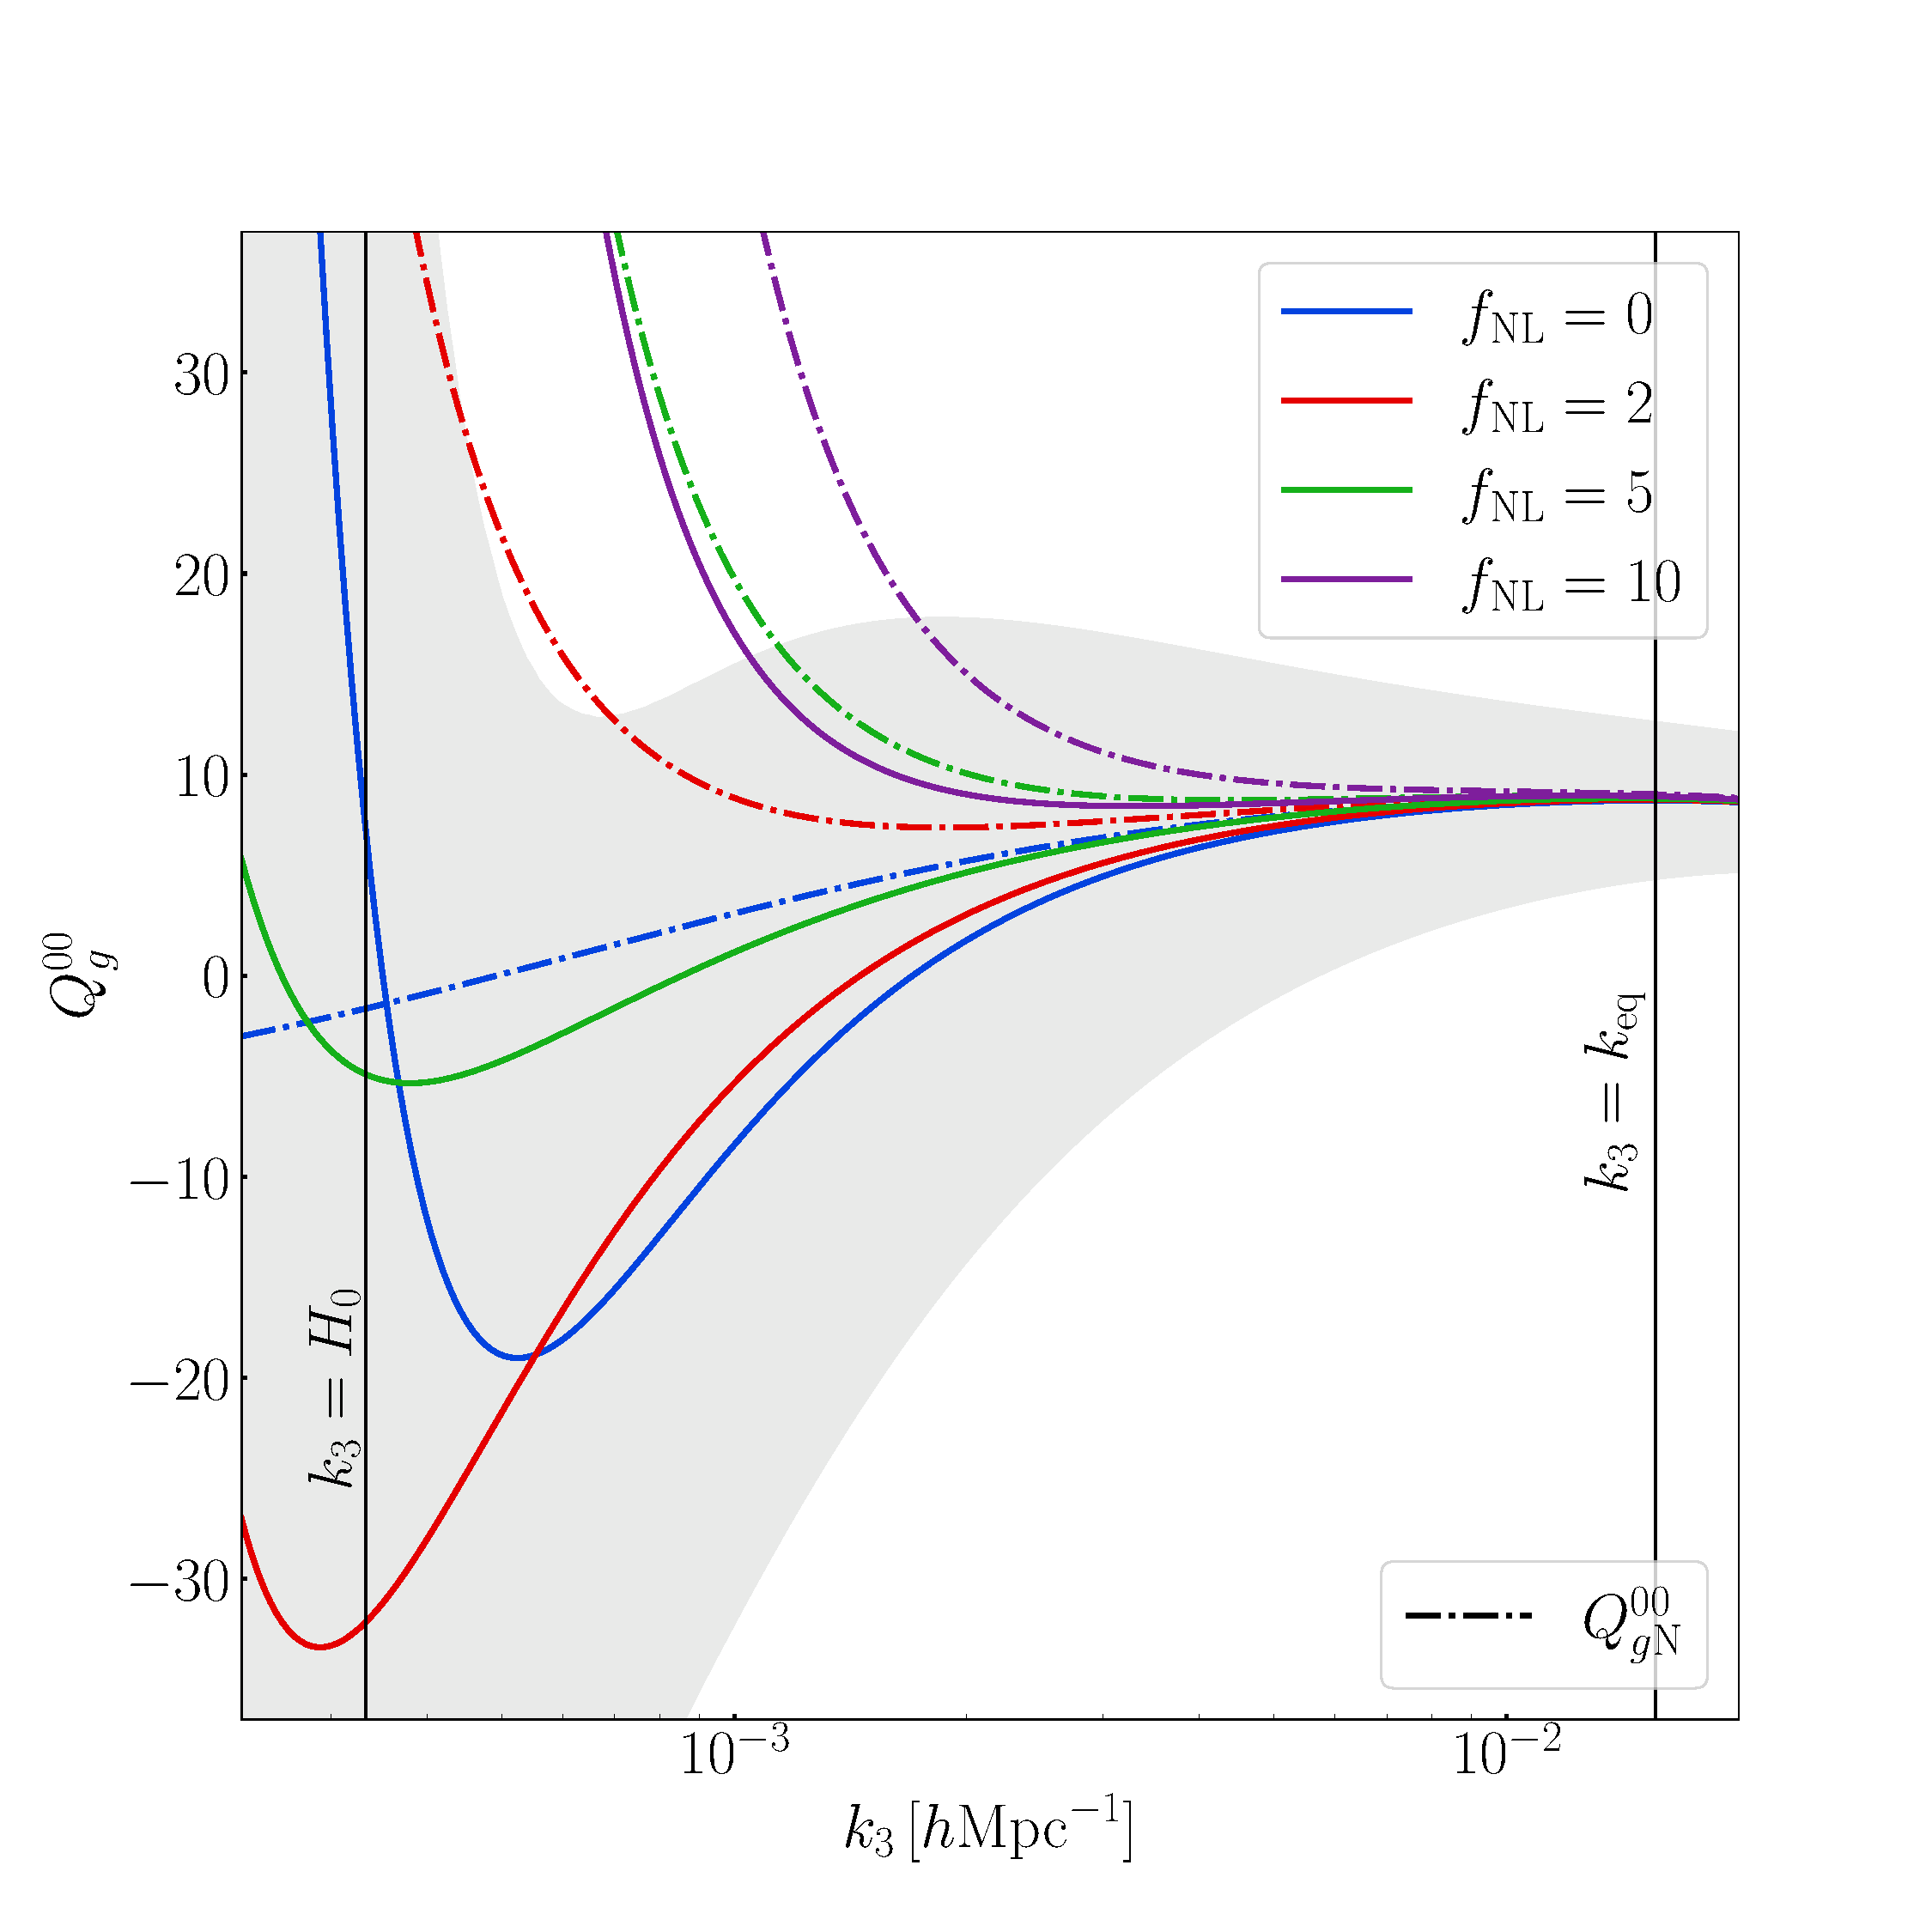
\includegraphics[width=0.49\textwidth]{fig/Q_k0_1_noShotnoise1.pdf}
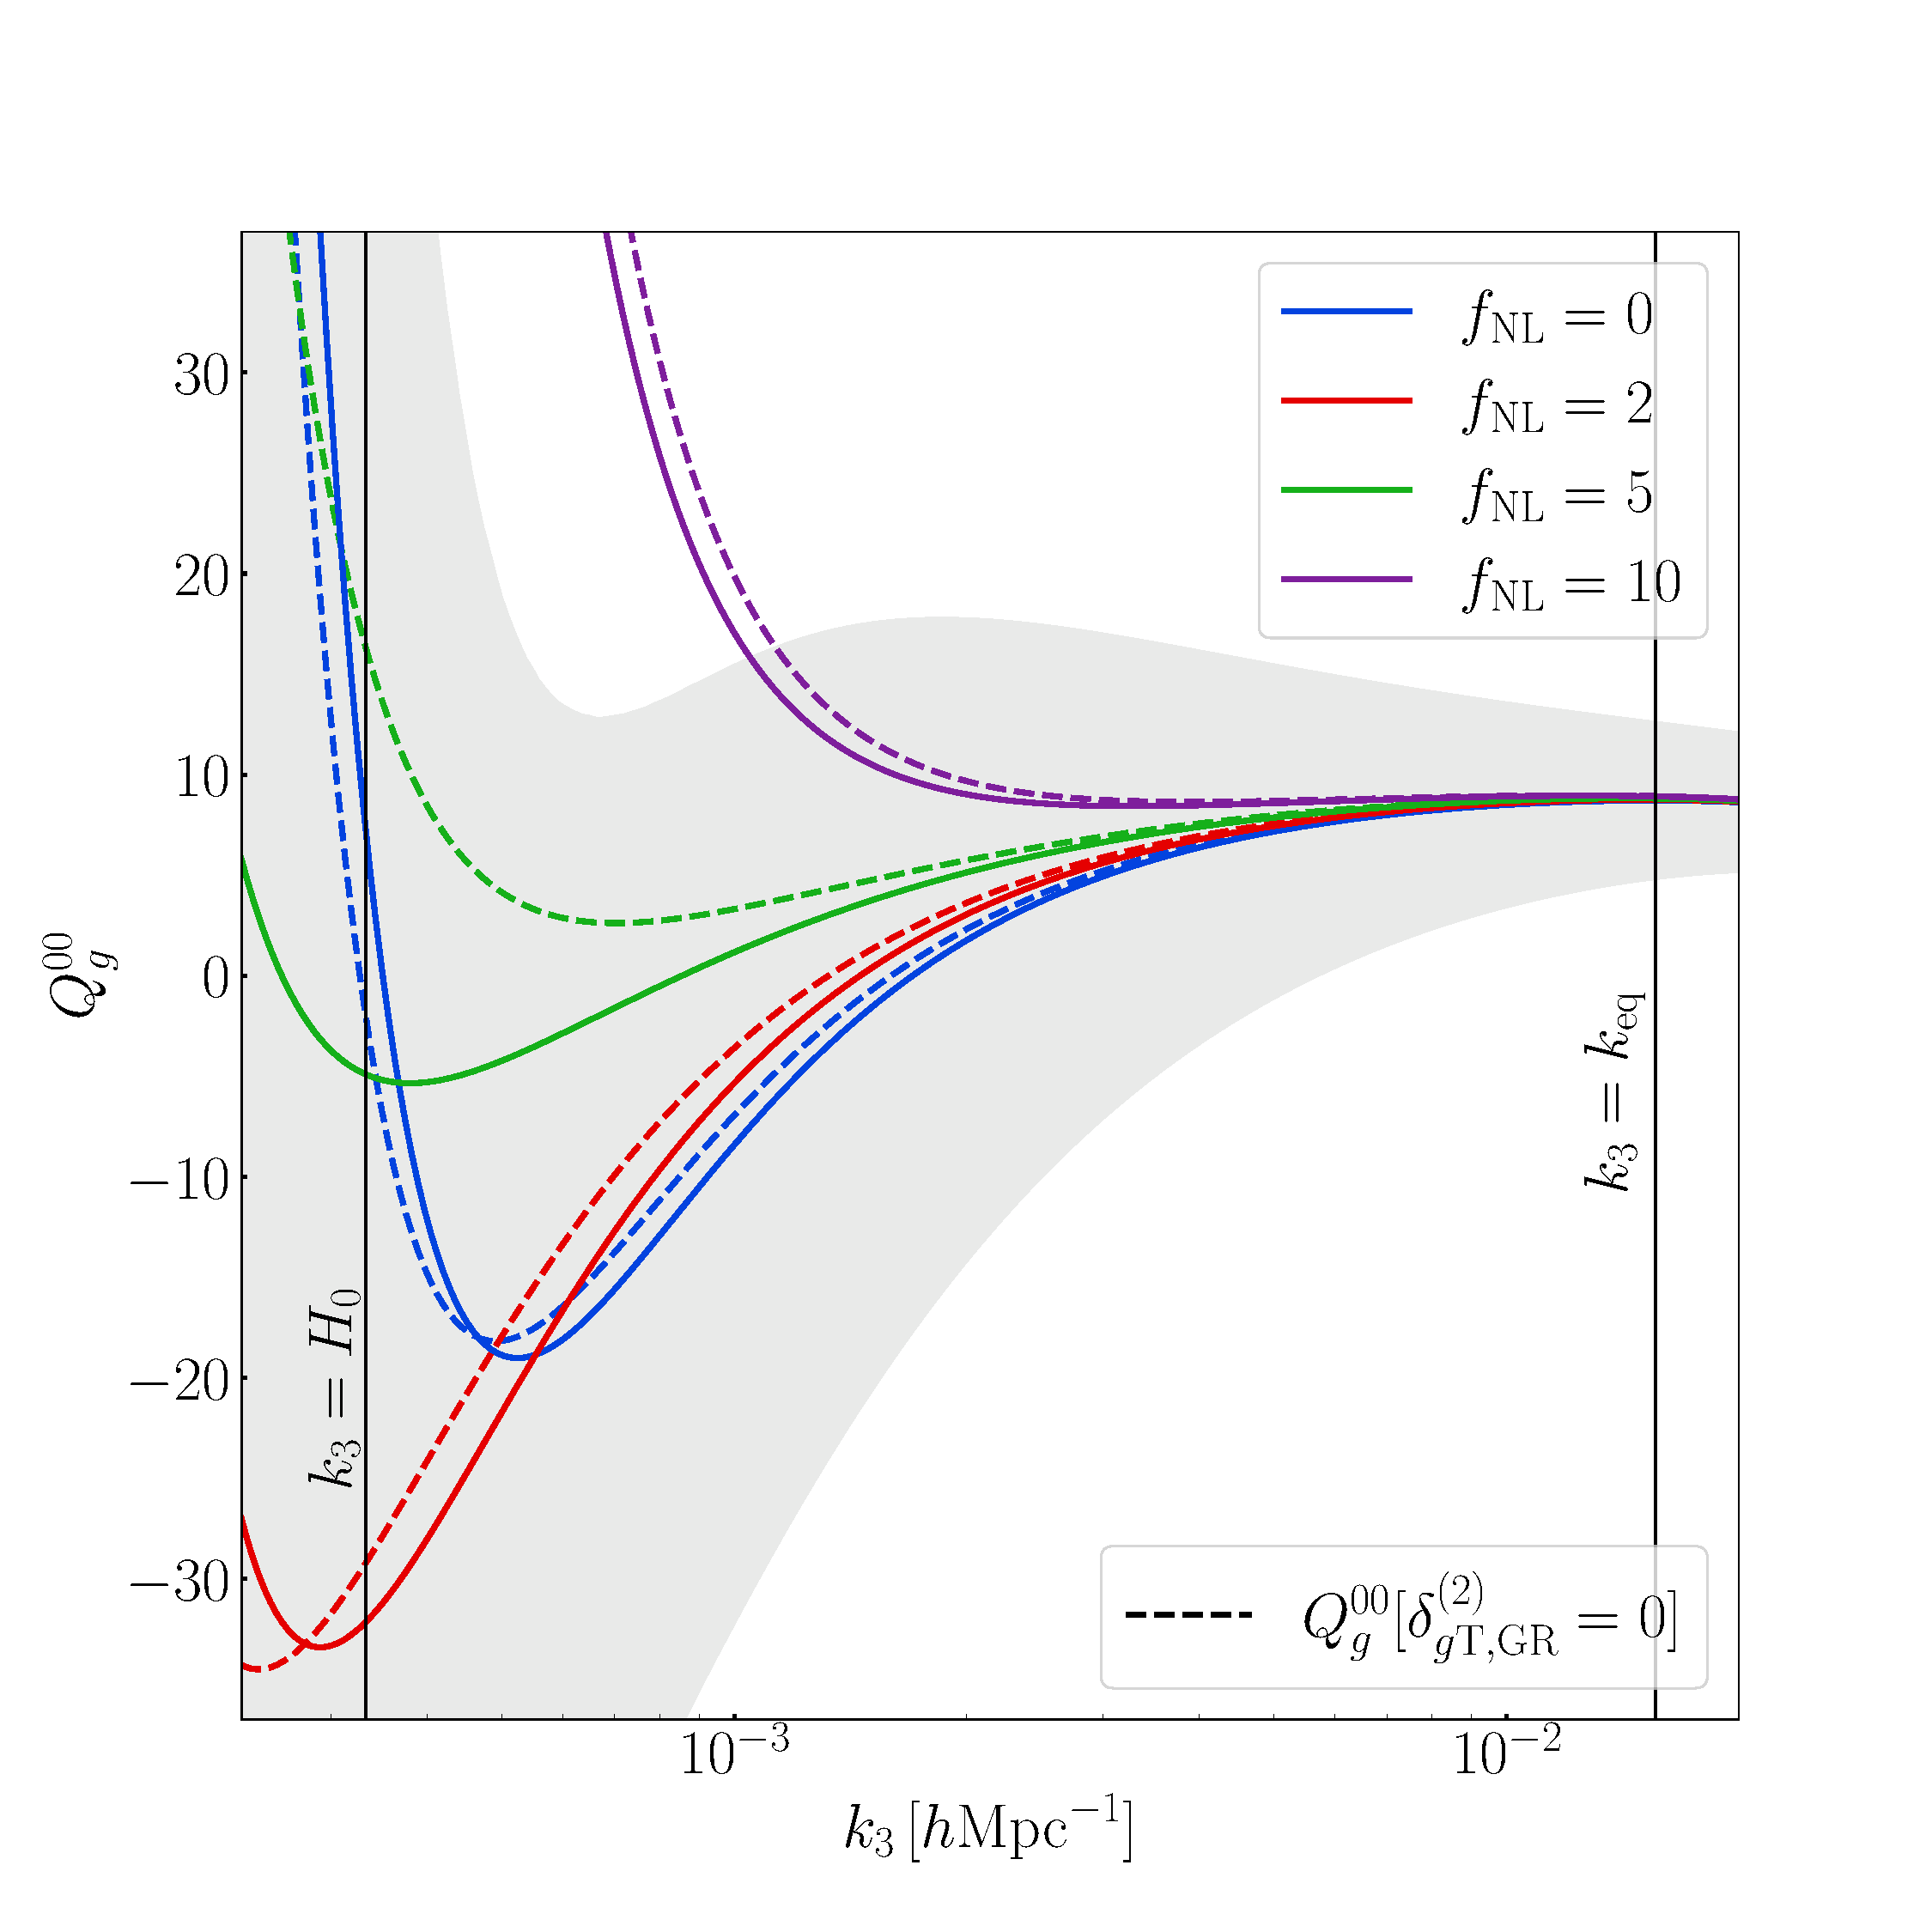
\includegraphics[width=0.49\textwidth]{fig/Q_k0_1_noShotnoise2.pdf}
\caption{ {Monopole of the reduced bispectrum for a Stage IV H$\alpha$ survey at $z=1$,  for various $\fnl$, with $k_1=k_2=0.1\,h$/Mpc. 
Shading indicates the 1$\sigma$ uncertainty (neglecting shot noise) for the $\fnl=0$ case (solid blue curve).
{\em Left:} Comparing the full relativistic monopole to the Newtonian approximation (dash-dot curves).   {\em Right:} Comparing the full relativistic monopole to the monopole without the GR correction to second-order  galaxy bias, \eqref{dtgr2} (dashed curves). }}
\label{qmono}
\end{figure}

The shading in Figure~\ref{qmono} is defined by the cosmic variance limited error $\sigma_{B}$ on the $\fnl=0$ monopole, given by \cite{Gagrani:2016rfy}: 
\begin{equation}
{\big(\sigma_{B}\big)^2=\frac{{\cal V}^{\,\mathrm{com}}}{\pi k_1k_2 k_3\, \Delta k}\,
\int \ud \mu_1\, \ud \phi \,P_g(k_1,\mu_1) \,P_g(k_2,\mu_2)\, P_g(k_3,\mu_3)}
\,,\label{sigb}
\end{equation}
where the galaxy power spectrum, from \eqref{kn}--\eqref{e2.14}, is
\begin{equation}
{P_g(k_a,\mu_a)=  \left| b_{10}
%+{b_{01} \over {\cal M}(k_a)} 
+f\mu_a^2+ \frac{\gamma_2}{k_a^2} +{\i}\,\mu_a \frac{\gamma_1}{k_a}\right|^2P(k_a)}\,. \label{pg0}
% \bigg[P^0_g(k_1)+ {1 \over n_g^{\rm com}} \bigg]  \bigg[P^0_g(k_2)+ {1 \over n_g^{\rm com}} \bigg]  \bigg[P^0_g(k_3)+ {1 \over n_g^{\rm com}} \bigg],
\end{equation}
In \eqref{sigb}, ${\cal V}^{\,\mathrm{com}}$ is the comoving volume of the redshift bin, $\Delta k$ is chosen as the fundamental mode, $2\pi ({\cal V}^{\,\mathrm{com}})^{-1/3}$, $k_1=k_2=0.1\,h$/Mpc, and \cite{Clarkson:2018dwn} $\mu_2=\mu_1\cos\theta_{12}+\sqrt{1-\mu_1^2}\sin\theta_{12}\,\cos\phi$, $\mu_3=-(k_1\mu_1+k_2\mu_2)/k_3$. Here $\theta_{12}$ is the {tail-to-tail} angle between $\k_1$ and $\k_2$, so that the squeezed limit is $\theta_{12}=\pi$.

The majority of curves corresponding to the different values of $\fnl$ plotted in Figure~\ref{qmono} fall within the shaded region. This means that these curves fall within the uncertainty region for $\fnl = 0$, and would be indistinguishable. Only for higher values $\fnl$, one can see a departure from the shaded area when going towards larger scales, and would potentially be distinguishable from the $\fnl = 0$ case. However, one should keep in mind the Planck 2018 constraints suggesting a small negative value for $\fnl$ as mentioned first in the Introduction chapter to this thesis~\ref{chapter:introgen}. 


\begin{figure}[ht]
	\centering
	\includegraphics[width=\textwidth]{fig/redB_lineandlake_v3.pdf}
\caption{Monopole of reduced bispectrum for isosceles triangles, as in Figure \ref{qmono}. {\em Left:} As a function of $\fnl$, for various values of $\theta\equiv\theta_{12}$, where $\theta=\pi$ is the squeezed limit. Dashed curves indicate negative values. {\em Right:} 2D colour map  as a function of $\fnl$ and $\theta/\pi$.}\label{rb2d}
\end{figure}
\begin{figure}[ht]
\centering
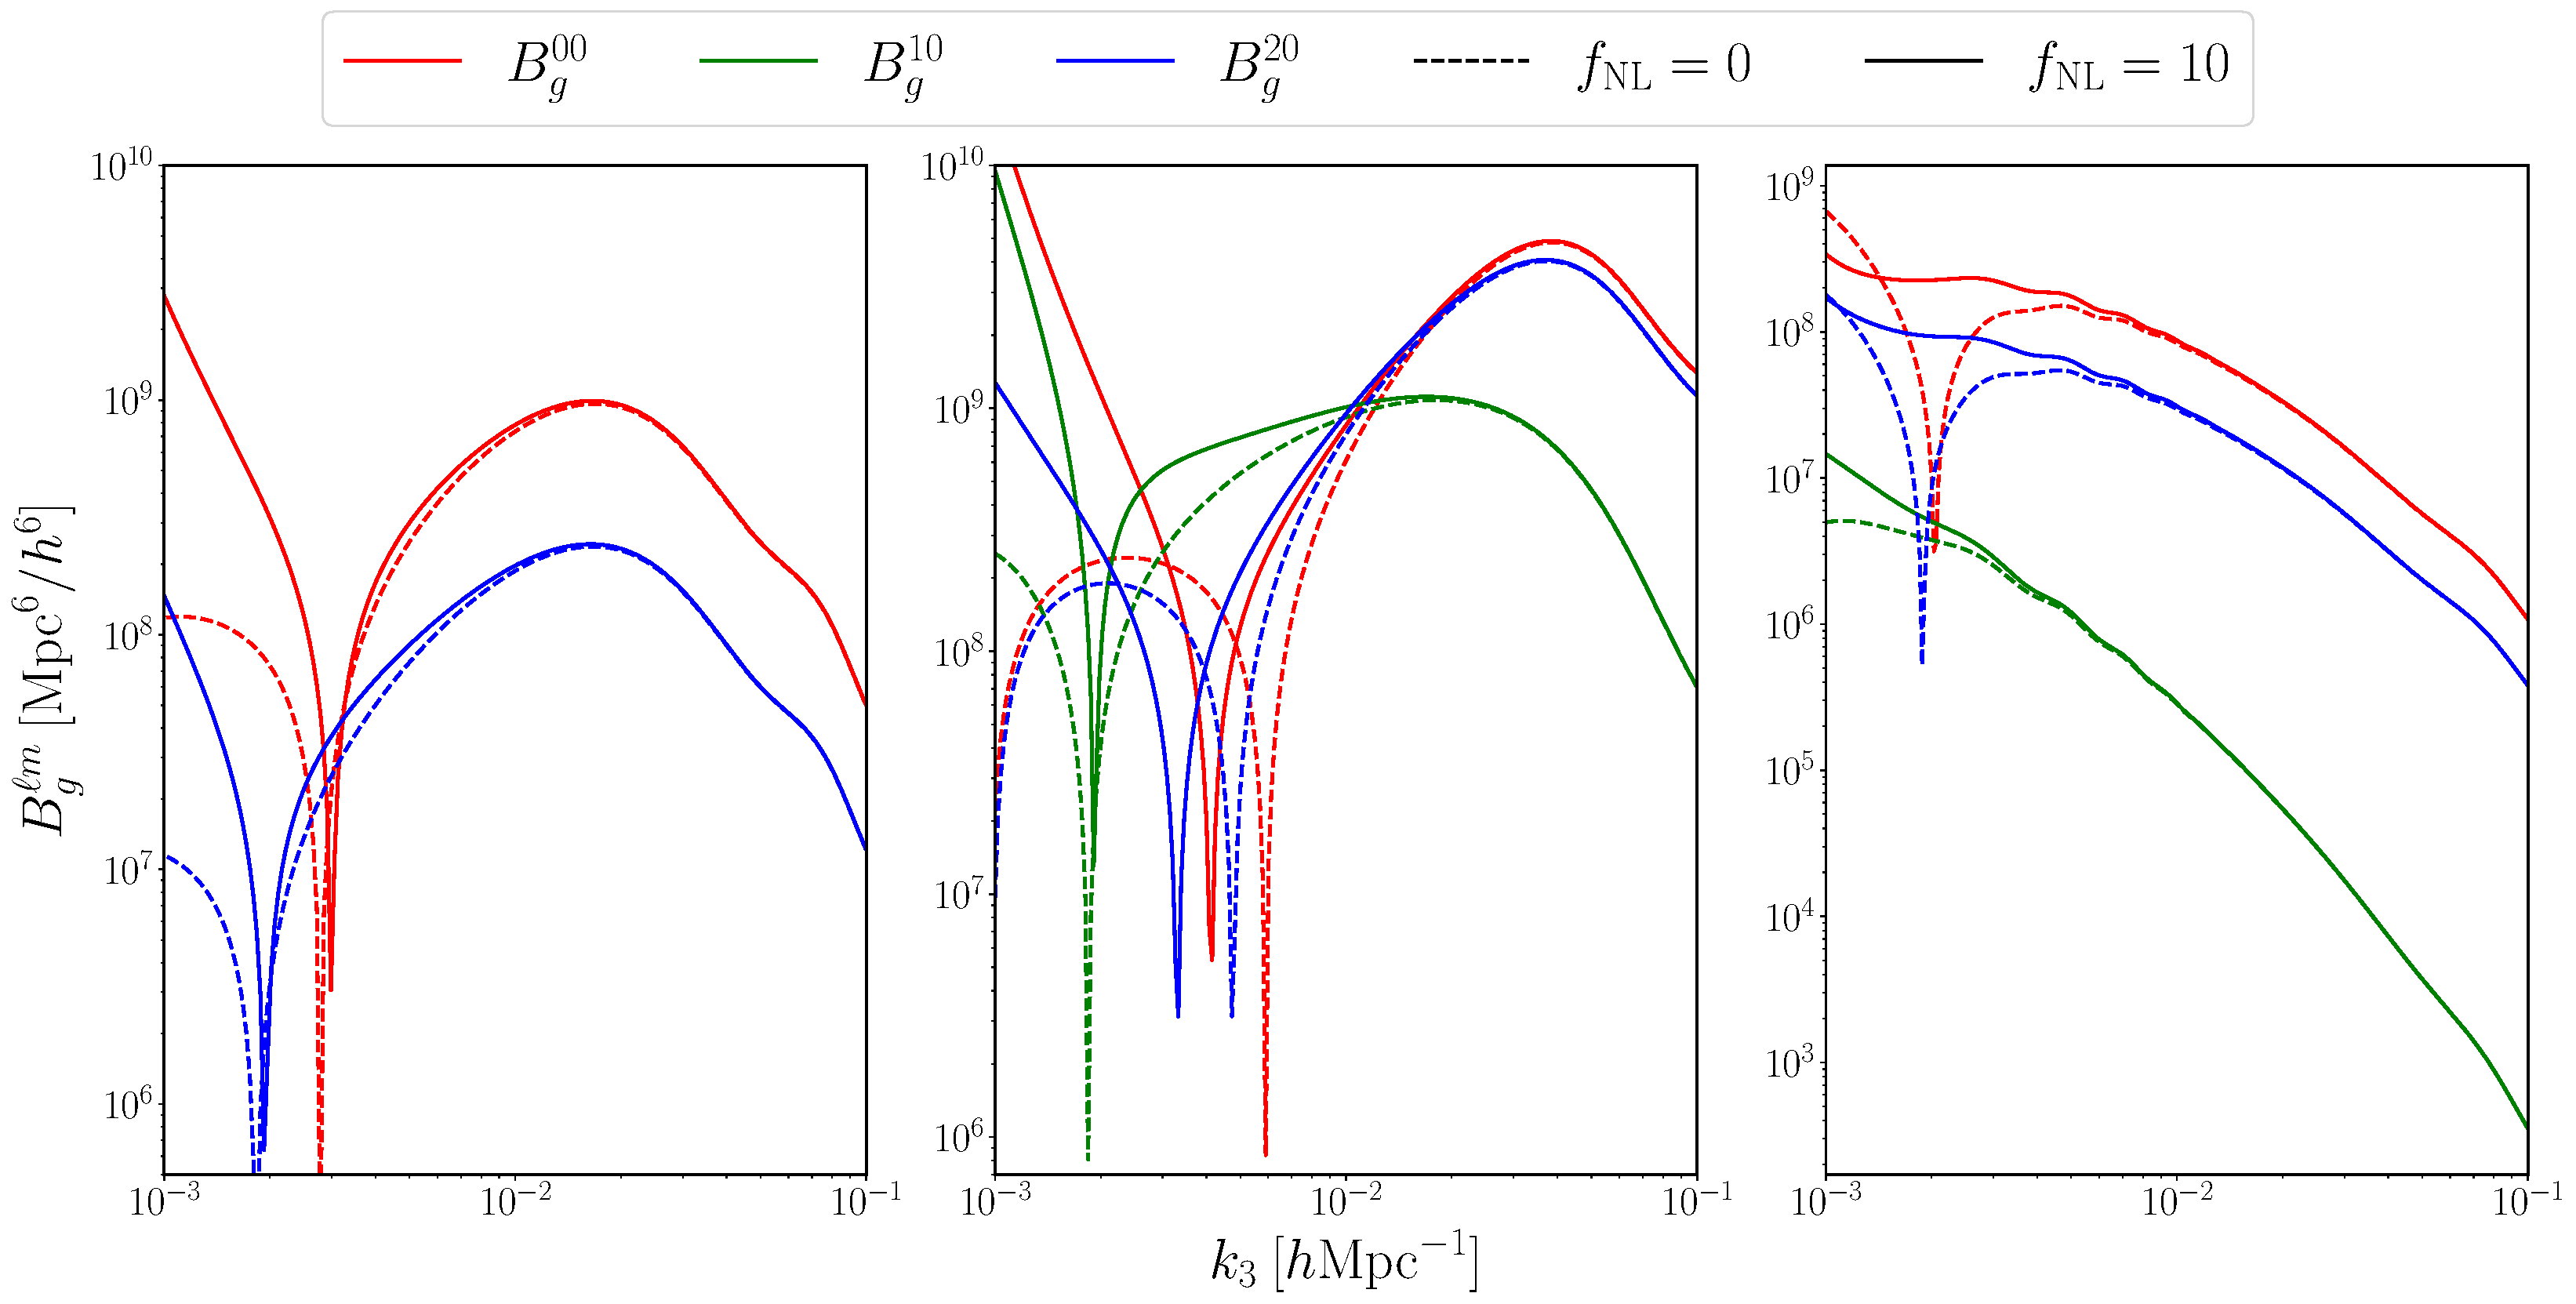
\includegraphics[width=\textwidth]{fig/multipoles_allpanels_v3.pdf}
\caption{First few nonzero multipoles for fixed triangle shape as a function of $k_3$, with {$\fnl=10$ (solid) and $\fnl=0$} (dashed).
{\em Left:} Equilateral configuration, $k_1=k_2=k_3$. {\em Middle:} Flattened configuration, $k_1=k_2\approx k_3/2$, with $\theta_{12}=2\degree$. {\em Right:} Squeezed configuration with $\theta_{12}=178\degree$ and $k_1=k_2=k_3/(2\sin \theta_{12})\approx 14\, k_3$.}
\label{eqfl}
\end{figure}

The effect of $\fnl$ is strongest in the monopole and competes with the GR contribution on ultra-large scales, since they both affect the Newtonian Gaussian bispectrum at ${\cal O}(\mathcal{H}^{2} / k^{2})$. We see this in Figure \ref{qmono} left panel, which shows the monopole of the reduced bispectrum for an increasingly squeezed isosceles triangle. 
In the Gaussian case (blue) we see that the Newtonian reduced monopole (dot-dash blue) becomes negative when the long mode is close to the Hubble scale, due to the effects of second-order galaxy bias.
The Gaussian GR correction to the Newtonian approximation is negative for super-equality long modes until close to the Hubble scale (this was pointed out in  \cite{Jolicoeur:2018blf}). GR effects drive the reduced monopole (solid blue) below zero for $H_0 \lesssim k_3\lesssim 0.002\,h$/Mpc  (the locations of the zero-crossings  are dependent on the Gaussian bias parameters, evolution bias and magnification bias). 

As $\fnl$ is increased above zero, the amplitude of the Newtonian reduced monopole (dot-dash curves) increases monotonically. When GR effects are taken into account, the reduced monopole is pushed upwards, but remains negative on observable scales for $\fnl \lesssim 5$, until it becomes always positive for $\fnl>5$   -- the precise turnaround value of $\fnl$ depends on astrophysical parameters. This means that for  $\fnl \lesssim 5$, 
local PNG {\em decreases} the amplitude of the reduced monopole on observable scales, in contrast to the Newtonian approximation. Comparing the green solid and blue dot-dash curves shows that {\em the Newtonian approximation is very close to the true reduced monopole with $\fnl \sim 5$}. For a universe with $\fnl \sim 5$, a Newtonian analysis of the squeezed bispectrum would conclude that the primordial universe is Gaussian. Similarly, a universe with $\fnl \sim 10$ would appear to have $\fnl \sim 5$ in a Newtonian approximation.
%For $\fnl>5$, local PNG and GR corrections act in the same direction. 

The GR contribution to the monopole is made up of: ${\cal O}(\mathcal{H}^{2} / k^{2})$ Gaussian projection terms, ${\cal O}(\mathcal{H}^{2} / k^{2})$  second-order galaxy bias correction (the same for Gaussian and PNG cases) and ${\cal O}(\mathcal{H}^{4} / k^{4})$ second-order local PNG contributions from GR projection effects.  The last contribution is effectively negligible on observable scales.
In the right panel of Figure \ref{qmono} we show that the GR bias correction is dominated by the Gaussian GR projection terms:  the effect of removing the GR correction to second-order galaxy bias is small. Note that the GR bias correction has a similar effect to a small negative value of $\fnl$.

In Figure \ref{rb2d}  we include  negative $\fnl$ and explore how  local PNG changes the monopole of the reduced bispectrum as we approach the squeezed limit, $\theta_{12}\to\pi$. For $\fnl\geq0$, the results provide a different perspective on Figure \ref{qmono} left panel. For negative $\fnl$, local PNG and GR effects act together to drive the monopole negative, so that the zero-crossing of the monopole occurs for smaller $\theta_{12}$, equivalently larger $k_3$. 
%This new effect would not be present without the inclusion of the GR contribution.

Figure \ref{eqfl} shows the effect of $\fnl$ on
the first three multipoles of the relativistic galaxy bispectrum, also including equilateral and flattened triangle shapes.
 In general, the Newtonian RSD effect induces only even multipoles, while the GR corrections modify the even multipoles and induce new odd multipoles. We show here the $m=0$  dipole (absent without GR corrections) and quadrupole (mainly Newtonian), compared to the monopole. 
 
 For the equilateral shape (left panel), the dipole vanishes exactly in the Gaussian case  \cite{Clarkson:2018dwn,deWeerd:2019cae} and nonzero $\fnl$ does not changes this result. The effect of $\fnl$ on the quadrupole is very similar to the case of the monopole. 
 
 For the flattened shape (middle panel), the dipole is the dominant part of the bispectrum for $0.002 \lesssim k_3/(h {\mathrm{Mpc}}^{-1})\lesssim 0.01$, and we see that $\fnl>0$ increases this effect further. The dipole $B_g^{1m}$ is purely relativistic: it vanishes in the Newtonian approximation  \cite{Clarkson:2018dwn,Maartens:2019yhx,Jolicoeur:2020eup}. 
 
 Finally, in the squeezed case (right panel), the effect on the monopole of  $\fnl=10$ is consistent with Figure \ref{qmono}. The quadrupole has a similar behaviour, and dominates the dipole. It is interesting that the three multipoles are approximately equal at scales near $k= 0.002\,h$/Mpc. Once again, this value is sensitive to astrophysical parameters.
%
%\SI{0.1}{\mega\parsec\tothe{-1}}
%---------------------------------------------------------------------------
%
%
\section{Conclusions}\label{sec4}
Upcoming galaxy surveys  and 21cm intensity mapping surveys will deliver high-precision cosmological measurements and constraints, based on a combination of the power spectrum and bispectrum. This advance demands a commensurate advance in theoretical precision. Here we contribute to the development of theoretical precision by deriving for the first time the local relativistic corrections to the tree-level redshift-space bispectrum in the presence of local primordial non-Gaussianity (PNG).

At first order in perturbations, there are no relativistic corrections to the comoving matter and galaxy density contrasts -- and therefore no correction to the galaxy clustering bias relation.  There are also no relativistic corrections to the velocity and metric potentials.  Consequently, there is no relativistic contribution to local PNG. The only relativistic correction is to the Newtonian projection effect, i.e. standard redshift-space distortions (RSD). 

At second-order, relativistic corrections go beyond projection effects to alter the galaxy bias relation and local PNG in the galaxy bispectrum. In summary, there are: 
\begin{itemize}
\item
relativistic projection corrections to the Newtonian RSD at first and second order;
\item
relativistic corrections to the Newtonian bias model in the comoving frame at second order;
\item
 second-order relativistic projection  corrections to the local PNG carried by Newtonian RSD -- from a coupling of first-order scale-dependent bias to first-order relativistic projection effects,  and from the linearly evolved local PNG in second-order velocity and metric potentials. 
 \end{itemize}

Our previous work \cite{Umeh:2016nuh,Jolicoeur:2017nyt, Jolicoeur:2017eyi, Jolicoeur:2018blf,Clarkson:2018dwn,Maartens:2019yhx,deWeerd:2019cae, Jolicoeur:2020eup} presented local (non-integrated) relativistic effects in the case of primordial Gaussianity and without the relativistic correction to galaxy bias. We have made corrections to these earlier results. In addition,  we have presented for the first time the galaxy bispectrum with relativistic corrections to galaxy clustering bias and new local PNG contributions that are encoded in relativistic projection effects.
Our main results are given  in Fourier space in \eqref{e2.15}--\eqref{e2.35}, with further details in Appendices \ref{app_betatables} and \ref{app_pngb}.

In Figures \ref{qmono} and \ref{rb2d}  we show examples of the squeezed monopole of the  reduced relativistic bispectrum for a Stage IV H$\alpha$ survey similar to Euclid, using physical models for the astrophysical parameters (clustering biases, evolution bias, magnification bias). These figures reveal various interesting relativistic features. In particular, they show  the bias in the estimate of $\fnl$ from using a Newtonian analysis. This bias is given by
\begin{equation}
\fnl^{\mathrm{Newt}} = \fnl + \Delta \fnl\,.
\end{equation}
For the Stage IV survey at $z=1$, the bias can be roughly estimated by eye as $\Delta \fnl\sim 5$, for the long mode above the equality scale. Although the precise level of bias is sensitive to astrophysical parameters and redshift, the point is that next-generation precision demands that relativistic corrections are included in the bispectrum.

\bro{In common with nearly all work on the Fourier-space bispectrum with RSD and PNG, we implicitly make a flat-sky assumption, based on the fixed global direction $\bm n$.  
As a consequence, wide-angle correlations are not included, so that the flat-sky analysis loses accuracy as $\theta$ increases, where $\theta$ is the maximum opening angle to 
the three-point correlations at the given redshift. This leads to a systematic bias in the separation of observational effects from the PNG signal, and therefore in the best-fit value  of $\fnl$.
 Including wide-angle effects  is a key target for future work. 
Corrections to the global flat-sky analysis of  the Fourier bispectrum can be made by using a local or `moving' line of sight  \cite{Scoccimarro:2015bla,Sugiyama:2018yzo,Shirasaki:2020vkk}.
However, corrections of this type are approximate and do not incorporate all the wide-angle effects. Ultimately, one needs to use the full-sky 3-point correlation function or the full-sky angular bispectrum (see e.g. \cite{Kehagias:2015tda, DiDio:2016gpd, DiDio:2018unb, Durrer:2020orn}) to properly include all wide-angle correlations. A major problem is that both of these alternatives are computationally more intensive. }
%---------------------------------------------------------------------------
%
\chapter{Fisher forecasts}
\label{chapter:fishers}

Mihi cordis gravitas \\
res videtur gravis; \\
iocus est amabilis \\
dulciorque favis; \\
quicquid Venus imperat, \\
labor est suavis, \\
quae numquam in cordibus \\
habitat ignavis.
% 
% !TEX root = ../thesis.tex

\chapter{Conclusions and Outlook}
\label{chapter:summary}
In this thesis, we have examined the relativistic contributions to the observed galaxy bispectrum. For the first part of this thesis, we focussed on the leading-order $\ord(\cH/k)$ corrections, which are absent in the power spectrum of a single tracer, but present in the bispectrum of single tracers and hence form a unique relativistic signature. In the second part of this thesis, we examined the higher-order relativistic corrections, and included local primordial non-Gaussianity in our theoretical description of the galaxy bispectrum. Local PNG and relativistic corrections have similar signatures ($k$-dependence) on large scales. Since detecting primordial non-Gaussianity is a key aim of next-generation (Stage IV) LSS surveys, it is crucial to include both relativistic effecs and PNG in the theoretical description of the observed bispectrum, in order to avoid misinterpreting measurements.

In Chapter~\ref{chapter:introgen}, we introduced the standard model of cosmology, $\Lambda$CDM, which is assumed throughout this work. We descibed the history of observational cosmology, and introduced two statistical tools that are employed to extract information from galaxy surveys: the power spectrum and the bispectrum, the latter of which is the main focus of this work. We briefly introduced primordial non-Gaussianity of the local type, which corresponds to squeezed shape triangles and is predicted by a wide range of inflationary scenarios. PNG gives rise to scale dependence in the galaxy bias, which we discussed next. This scale dependence comes in at next-to-leading-order in $\cH/k$, and motivates the need for inclusion of relativistic corrections.

In Chapter~\ref{chapter:dipole}, we analyse the $\cH/k$ effects in the bispectrum. We have shown that the relativistic galaxy bispectrum has a leading-order correction, which gives rise to a local dipole with resprect to the observer's line-of-sight. This dipole exists even for the bispectrum of a single tracer, in contrast with the power spectrum. Even on equality scales, at redshift $z=1$, the amplitude of this dipole is about 10\% of that of the monopole. Although we have used Gaussian initial conditions in these predicitons, the dipole will be unaffected by non-Gaussianity at leading order, since these corrections start at $\ord(\cH^2/k^2)$. As such, the dipole of the bispectrum is a unique signature of GR on cosmological scales, and offers a new observational window into modifications of GR.

In Chapter~\ref{chapter:detect}, we continue our consideration of the leading-order corrections first examined in Chapter~\ref{chapter:dipole}. Since the relativistic contribution to the bispectrum couples to short-scale Newtonian terms, the signal is not confined to very large scales, unlike the case of the power spectrum. We confirmed the expectations of detectability of such a signal by showing that the signal-to-noise ratio on this relativistic part is $\ord 10$ for a Stage IV H$\alpha$ spectroscopic survey similar to \emph{Euclid}. We checked that the detectability is not compromised by including the uncertainties on two cosmological growth parameters, $\sigma_8$ and $\gamma$, assuming that other cosmological and nuisance parameters are determined by the Newtonian power spectrum and bispectrum. 

The relativistic SNR is dependent on the $k_\mathrm{max}$ assumed, i.e. on the small scales where perturbation theory breaks down, because of the coupling of the relativistic effects to short-scale Newtonian terms. Further, the SNR depends on the largest available scales too, although not as strongly. Little signal is lost if $k_\mathrm{min}$ is increased.  In contrast, the SNR more strongly depends on accurate modelling of the second-order part of the relativistic correction, and in particular is dependent on two astrophysical parameters that do not appear in the Newtonian approximation: the evolution and magnification bias parameters $b_e$ and $\Q$. A key feature of this work was the inclusion of physically self-consistent derivations of these quantities from the luminosity function, which we did for two luminosity function models relevant for future H$\alpha$ surveys.

HI intensity mapping surveys require significant additions to deal with foreground contamination and complexities of instrumental noise, which dominates over shot noise. The loss of signal due to foreground cleaning and telescope beam effects reduces the SNR for next-generation IM surveys on MeerKAT, SKA1-MID and HIRAX, with marginally detectable SNR forecasts of $\sim 6$ for SKA1 and $\sim 5$ for HIRAX. The PUMA survey, which is still in proposal stage, would deliver a SNR of $\sim 14$ in its Petite or first phase (before the futuristic full survey). 

In Chapter~\ref{chapter:ho}, we summarised past work on the Fourier-space galaxy bispectrum including all orders of relativistic projection effects in the observed bispectrum. This meant going beyond the leading-order relativistic correction that was considered in the previous chapters. We included an overview of how the Fourier-space bispectrum of galaxies is constructed from observed galaxy overdensities, and motivate the inclusion of these higher order GR corrections, as they mimic the signal of PNG on large scales. We also showed that corrections that arise from vector and tensor modes are subdominant compared to scalar contributions, and hence can safely be ignored.

Next, in Chapter~\ref{chapter:multipoles}, we present a full analytic decomposition of the Fourier space bispectrum into invariant multipoles about the observer's line-of-sight. We have found that relativistic corrections generate a hierarchy of odd multipoles, which are absent in the Newtonian picture. They also contribute to even multipoles. The leading power of the relativistic correction in each $\ell$ harmonic is $(\cH/k)^1$ for odd multipoles and $(\cH/k)^2$ for even multipoles. We have found that the co-linear configuration only generates non-zero $m = 0$ multipoles, and vanishes for all other values of $m$. Equilateral configurations are always zero for odd $m$, and always zero for the special case of the dipole. Relative to the Newtonian monopole, we have found that all relativistic multipoles decay with redshift. Depending on the scales of interest, higher-order Newtonian terms can exceed second-order GR terms in amplitude. 

Finally, in Chapter~\ref{chapter:localpng}, we have presented the local relativistic corrections to the tree-level redshift-space bispectrum of galaxies in the presence of local PNG. In summary, there are: relativistic projection corrections to the Newtonian RSD at first and second order, relativistic corrections to the Newtonian bias model in the comoving frame at second order, and second-order relativistic projection corrections to the local PNG carried by Newtonian RSD-- from a coupling of first-order scale-dependent bias to first-order relativistic projection effects, and from the linearly evolved local PNG in second-order velocity and metric potentials. We have also shown the bias in the estimate of non-Gaussian parameter $\fnl$ from using a Newtonian analysis, which for a Stage IV survey at $z = 1$ is about $\Delta \fnl \sim 5$, for the long mode above the equality scale. The precise level of bias is of course sensitive to astrophysical parameters and redshift, but the key result is that next-generation precision demands that relativistic corrections are included in the bispectrum. 

Further work could take multiple different directions. Some lower-hanging fruits would be for example Fisher forecasts using the bispectrum to improve cosmological constraints, e.g. including $\fnl$ and scale-dependent bias. Due to the sensitivity of the bispectrum on evolution and magnification bias $b_e$ and $\Q$, it may offer potential for improved constraints on bias parameters. The bispectrum of multiple tracers is not yet fully understood either. The advantages and limitations of measuring parameters using the power spectrum of multiple tracers is already well understood, but it is unclear in what regimes and for what parameters the multi-tracer bispectrum would be a better suited observable. 

In terms of predictions for detectability, it is necessary to include the window function, which we have neglected to do in our Chapter~\ref{chapter:detect}. The window function can also have an imaginary part, similar to the leading-order relativistic correction to the bispectrum. This will need to be corrected for. The dipole that arises from the imaginary part of the bispectrum vanishes identically for equilateral triangle configurations, which may help disentangle the relativistic dipole from that of the window function. There is also no simulation-based model for the bispectrum RSD damping parameter, which we have taken to be equal to the power spectrum damping parameter. From testing the impact of increasing the bispectrum damping parameter, it leads to only a small change in our results, but a complete analysis would require a consistent model of bispectrum RSD damping.

In common with other work on the Fourier-space bispectrum, our analysis as presented here implicitly uses the plane-parallel approximation, since we have fixed the line-of-sight direction $\n$. This approximation can be avoided, for example by using a Fourier-Bessel analysis of bispectrum multipoles, but this will come at the cost of a significant increase in complexity. Note however that errors from the plane-parallel approximation are mitigated in high redshift surveys such as considered in this thesis.

Further work also needs to include the effects of lensing magnification, which are excluded in the standard Fourier analysis. These have been included in work on the galaxy angular bispectrum, and in a spherical Bessel analysis of the bispectrum. 

We also neglected cross-correlations among redshift bins throughout this thesis. This is justified by exquisite redshift accuracy in future surveys, which allows for sharp-edged redshift bins with little to no overlap between them. Integrated effects however will induce correlations along the line-of-sight direction. Ultimately, integrated effects and cross-bin correlations need to be included, which requires a complete treatment using the angular bispectrum or 3-point correlation function. The inclusion of integrated contributions may also change the impact that corrections due to vector and tensor modes have on the bispectrum, and may mean that these corrections can no longer be neglected.


%
\begin{appendices}
%
\chapter{Beta coefficients}
\label{app_betas}
%
\begin{align} 
\frac{\beta_{1}}{\mathcal{H}^{4}} &= \frac{9}{4}\Omega_{m}^{2}\Bigg[6-2f\bigg(2b_{e}-4\Q-\frac{4(1-\Q)}{\chi\cH}-\frac{2\cH'}{\cH^{2}}\bigg)-\frac{2f'}{\cH}+b_{e}^{2}+5b_{e}-8b_{e}\Q + 4\Q + 16\Q^{2} \nonumber\\ 
& - 16\frac{\p \Q}{\p \ln{\bar{L}}} - 8\frac{\Q'}{\cH} + \frac{b_{e}'}{\cH}+\frac{2}{\chi^{2}\cH^{2}}\bigg(1-\Q+2\Q^{2}-2\frac{\p \Q}{\p \ln{\bar{L}}}\bigg)
 \nonumber\\ 
& - \frac{2}{\chi\cH}\bigg(3+2b_{e}-2b_{e}\Q-3\Q +8\Q^{2}-\frac{3\cH'}{\cH^{2}}(1-\Q) -8\frac{\p \Q}{\p \ln{\bar{L}}} - 2\frac{\Q'}{\cH}\bigg) \nonumber \\
& + \frac{\cH'}{\cH^{2}}\bigg(-7-2b_{e}+8\Q+\frac{3\cH'}{\cH^{2}}\bigg) - \frac{\cH''}{\cH^{3}}\Bigg] \nonumber \\
&  +\frac{3}{2}\Omega_{m}f\Bigg[5-2f(4-b_{e})+\frac{2f'}{\cH}+2b_{e}\bigg(5+\frac{2(1-\Q)}{\chi\cH}\bigg)-\frac{2b_{e}'}{\cH} -2b_{e}^{2} + 8b_{e}\Q - 28\Q \nonumber \\
& - \frac{14(1-\Q)}{\chi\cH}-\frac{3\cH'}{\cH^{2}} +4\bigg(2-\frac{1}{\chi\cH}\bigg)\frac{\Q'}{\cH}\Bigg] \nonumber \\
&  +\frac{3}{2}\Omega_{m}f^{2}\bigg[-2+2f-b_{e}+4\Q+\frac{2(1-\Q)}{\chi\cH}+\frac{3\cH'}{\cH^{2}}\bigg] \nonumber \\
&  +f^{2}\bigg[12-7b_{e}+b_{e}^{2}+\frac{b_{e}'}{\cH}+(b_{e}-3)\frac{\cH'}{\cH^{2}}\bigg] - \frac{3}{2}\Omega_{m}\frac{f'}{\cH} \\
\nonumber\\
%----------------
\frac{\beta_{2}}{\cH^{4}} &= \frac{9}{2}\Omega_{m}^{2}\bigg[-1+b_{e}-2\Q-\frac{2(1-\Q)}{\chi\cH}-\frac{\cH'}{\cH^{2}}\bigg] + 3\Omega_{m}f\bigg[-1+2f{-b_{e}}+4\Q+\frac{2(1-\Q)}{\chi\cH}+\frac{3\cH'}{\cH^{2}}\bigg] \nonumber \\
&  +3\Omega_{m}f^{2}\bigg[-1+b_{e}-2\Q-\frac{2(1-\Q)}{\chi\cH}-\frac{\cH'}{\cH^{2}}\bigg] + 3\Omega_{m}\frac{f'}{\cH}\; \\ 
%----------------
\frac{\beta_{3}}{\mathcal{H}^{3}} &= \frac{9}{4}\Omega_{m}^{2}(f-2+2\Q) \nonumber \\
&  + \frac{3}{2}\Omega_{m}f\Bigg[-2 -f\bigg(-3+f+2b_{e}-3\Q-\frac{4(1-\Q)}{\chi\cH}-\frac{2\cH'}{\cH^{2}}\bigg)-\frac{f'}{\cH}\nonumber \\
& +{3}b_{e}+b_{e}^{2}-6b_{e}\Q{+4}\Q +8\Q^{2}-8\frac{\p \Q}{\p \ln{\bar{L}}} -6\frac{\Q'}{\cH} +\frac{b_{e}'}{\cH} \nonumber \\
& +\frac{2}{\chi^{2}\cH^{2}}\bigg(1-\Q+2\Q^{2}-2\frac{\p \Q}{\p \ln{\bar{L}}}\bigg) + \frac{2}{\chi \cH}\bigg({-1} -2b_{e}+2b_{e}\Q{+}\Q-6\Q^{2}  \nonumber \\
& +\frac{3\cH'}{\cH^{2}}(1-\Q) +6\frac{\p \Q}{\p \ln{\bar{L}}} + 2\frac{\Q'}{\cH}\bigg) -\frac{\cH'}{\cH^{2}}\bigg({3}+2b_{e}-6\Q-\frac{3\cH'}{\cH^{2}}\bigg) - \frac{\cH''}{\cH^{3}}\Bigg] \nonumber \\
&  {+} f^{2}\Bigg[-3+2b_{e}\bigg(2+\frac{(1-\Q)}{\chi\cH}\bigg)-b_{e}^{2}+2b_{e}\Q -6\Q-\frac{b_{e}'}{\cH}-\frac{6(1-\Q)}{\chi\cH}\nonumber \\
& +2\bigg(1-\frac{1}{\chi\cH}\bigg)\frac{\Q'}{\cH}\Bigg]  \\ 
%----------------
\frac{\beta_{4}}{\cH^{3}} &= \frac{9}{2}\Omega_{m}f\bigg[-b_{e}+2\Q+\frac{2(1-\Q)}{\chi \cH}+\frac{\cH'}{\cH^{2}}\bigg]\\ 
%----------------
{{\frac{\beta_5}{\cH^{3}}}} &= 3\Omega_{m}f\bigg[b_{e}-2\Q-\frac{2(1-\Q)}{\chi\cH}-\frac{\cH'}{\cH^{2}}\bigg] \\ 
%------
\frac{\beta_6}{\cH^{2}} &= \frac{3}{2}\Omega_{m}\Bigg[2-2f+b_{e}-4\Q-\frac{2(1-\Q)}{\chi\cH}-\frac{\cH'}{\cH^{2}}\Bigg] \\
%---------
\frac{\beta_7}{\cH^{2}} &= f(3-b_{e}) \\ 
%----------------
\frac{\beta_8}{\cH^{2}} &= {3\Omega_{m}f(2-f-2\Q)} + f^{2}\Bigg[4+b_{e}-b_{e}^{2}+4b_{e}\Q-{6}\Q-4\Q^{2}+4\frac{\p \Q}{\p \ln{\bar{L}}} + 4\frac{\Q'}{\cH} - \frac{b_{e}'}{\cH}  \nonumber \\\nonumber\\
& - \frac{2}{\chi^{2}\cH^{2}}\bigg(1-\Q+2\Q^{2}-2\frac{\p \Q}{\p \ln{\bar{L}}}\bigg) - \frac{2}{\chi\cH}\bigg(3-2b_{e}+2b_{e}\Q-\Q-4\Q^{2}+\frac{3\cH'}{\cH^{2}}(1-\Q) \nonumber\\
& + 4\frac{\p \Q}{\p \ln{\bar{L}}} + 2\frac{\Q'}{\cH}\bigg) - \frac{\cH'}{\cH^{2}}\bigg(3-2b_{e}+{4}\Q+\frac{3\cH'}{\cH^{2}}\bigg) + \frac{\cH''}{\cH^{3}}\Bigg] \\ 
%----------------
\frac{\beta_{9}}{\cH^{2}} &= -\frac{9}{2}\Omega_{m}f \\ 
%----------------
{\frac{\beta_{10}}{\cH^{2}}} &= 3\Omega_{m}f \\ 
%----------------
\frac{\beta_{11}}{\cH^{2}} &= 3\Omega_{m}\bigg(\frac{1}{2}+f\bigg) + f - f^{2}\Bigg[-1+b_{e}-2\Q- \frac{2(1+\Q)}{\chi\cH}-\frac{\cH'}{\cH^{2}}\Bigg] \\ 
%-----------------
\frac{\beta_{12}}{\cH^{2}} &= \frac{3}{2}\Omega_{m}\Bigg[-2+b_{1}\bigg(2+b_{e}-4\Q-\frac{2(1-\Q)}{\chi\cH} -\frac{\cH'}{\cH^{2}}\bigg) + \frac{b_{1}'}{\cH} + 2\bigg(2-\frac{1}{\chi\cH}\bigg)\frac{\p b_{1}}{\p \ln{\bar{L}}}\Bigg] \nonumber \\
&- f\Bigg[2+b_{1}(f-3+b_{e}) + \frac{b_{1}'}{\cH}\Bigg]  \\ 
%----------------
\frac{\beta_{13}}{\cH^{2}} &= \frac{9}{4}\Omega_{m}^{2} {+ \frac{3}{2}\Omega_{m}f\Bigg[1-2f+2b_{e}-{6}\Q-\frac{4(1-\Q)}{\chi\cH}-\frac{3\cH'}{\cH^{2}}\Bigg]} + f^{2}(3-b_{e}) \\ 
%----------------
\frac{\beta_{14}}{\cH} &= -\frac{3}{2}\Omega_{m}b_{1} \\
%----------------
\frac{\beta_{15}}{\cH} &= 2f^{2}  \\ 
%----------------
\frac{\beta_{16}}{\cH} &= f\Bigg[b_{1}\bigg(f+b_{e}-2\Q-\frac{2(1-\Q)}{\chi\cH}-\frac{\cH'}{\cH^{2}}\bigg) + \frac{b_{1}'}{\cH} + 2\bigg(1-\frac{1}{\chi\cH}\bigg)\frac{\p b_{1}}{\p \ln \bar{L}}\Bigg] \\
%----------------
\frac{\beta_{17}}{\cH} &= -\frac{3}{2}\Omega_{m}f \\
%----------------
\frac{\beta_{18}}{\cH} &= \frac{3}{2}\Omega_{m}f -f^{2}\Bigg[3-2b_{e}+{4}\Q+\frac{4(1-\Q)}{\chi\cH}+\frac{3\cH'}{\cH^{2}}\Bigg] \\
%----------------
\frac{\beta_{19}}{\cH} &= f\Bigg[b_{e}-2Q-\frac{2(1-\Q)}{\chi\cH}-\frac{\cH'}{\cH^{2}}\Bigg] 
\end{align}
%
\chapter{Beta coefficient tables}
\label{app_pnga}
%
% \begin{longtable}{| p{.20\textwidth} | p{.80\textwidth} |} 
% \caption{Your caption here}\\
% \hline
% foo & bar \\ \hline 
% foo & bar \\ \hline
% foo & bar \\ \hline
% foo & bar \\ \hline
% foo & bar \\ \hline
% foo & bar \\ \hline
% foo & bar \\ \hline
% foo & bar \\ \hline
% foo & bar \\ \hline
% foo & bar \\ \hline
% foo & bar \\ \hline
%  % needs to go inside longtable environment
% \label{tabc1}
% \end{longtable}

Here we present a table of individual terms in the observed density fluctuation $\Delta_g^{(2)}$, with the corresponding $\beta$ function $\beta_I$ in the second column (N for standard Newtonian terms), Fourier space kernel $\mathcal{F}$, and the coefficients of the terms that appear in $\Delta_g^{(2)}$ in the fourth column. 

\begingroup
\tiny
\begin{longtable}{| c | c | c | c |} 
\caption{ {Individual terms in the observed $\Delta_g^{(2)}(a,\bm{x})$ [see \eqref{eq:SecondorderNewtonian}, \eqref{odg2}] for $\fnl=0$ are shown in column 1. The related $\beta_I$ functions in \eqref{e2.23} are listed in column 2. The Fourier-space kernels ${\cal F}$  corresponding to column 1, given by 
$ \int \!{\ud \k'}\, {\cal F}(\k',\k-\k')\delta_{\mathrm{T}}(\k')\delta_{\mathrm{T}}(\k-\k')/(2\pi)^3$, are shown in column~3. Column 4 gives
the coefficients of the terms in $\Delta_g^{(2)}$ (column 1). The line-of-sight derivative is $\partial_\|=\bm{n}\!\cdot\!\bm{\nabla}$ and $\Phi=\Psi$.
The superscript (1) on first-order quantities has been omitted and N denotes Newtonian. This table updates the one in \cite{Jolicoeur:2017nyt}.}} \label{tabc1} \\
\hline 
&  &  & \\
TERM & $~~\beta~~$ & FOURIER KERNEL    & COEFFICIENT \\ 
&  &  & \\ \hline \hline
&  &  & \\
%%----------------------- Newtonian
$\delta^{(2)}_{\mathrm{T,{N}}}$ & N & $F_{2}(\!\bm{k}_{1},\!\bm{k}_{2}\!)$ & $b_{10}$ \\ 
&  &  & \\
%%-----------------------
${\big(\delta_{\mathrm{T}}\big)^2}$ & N & 1 & $b_{20}$ \\ 
&  &  & \\
%%-----------------------
${s^2}$ & N & $S_2(\!\bm{k}_{1},\!\bm{k}_{2}\!)$ & $b_{s}$ \\ 
&  &  & \\
%%-----------------------
$\partial_{\parallel}^{2}V^{(2)}_{{\mathrm{N}}}$ & N & $f^{2}\cH \mu_{3}^{2}G_{2}(\!\bm{k}_{1},\!\bm{k}_{2}\!)$ & $-1/\cH$ \\ 
&  &  & \\
%%-----------------------
$\delta_{\mathrm{T}}\partial_{\parallel}^{2}V$ & N & $-f\cH \big(\mu_{1}^{2} + \mu_{2}^{2}\big)/2 $ & $-2b_{10}/\cH$ \\
&  &  & \\ 
%%-----------------------
$\partial_{\parallel}V \partial_{\parallel}\delta_{\mathrm{T}}$ & N\ & $-f\cH {{\mu_{1}\mu_{2}\big(k_{1}^{2} + k_{2}^{2}\big)}/{\big(2k_{1}k_{2}\big)}}$& $-2b_{10}/\cH$ \\ 
&  &  & \\
%%-----------------------
$\partial_{\parallel}V \partial_{\parallel}^{3}V $  & N & $f^{2} \cH^2{{\big(\mu_{1}\mu_{2}^{3}k_{2}^{2} + \mu_{2}\mu_{1}^{3}k_{1}^{2}\big)}/{\big(k_{1}k_{2}\big)}}$ & $ {2}/{\cH^{2}}$  \\
&  &  & \\ 
%%-----------------------
$\big[\partial_{\parallel}^{2}V\big]^{2}$  & N &$f^{2}\cH^2 \,\mu_{1}^{2}\mu_{2}^{2}$ & ${2}/{\cH^{2}}$ \\ 
&  &  & \\
\hline 
&  &  & \\
%%----------------------- beta_{1}, beta_{2}
$\big(\Psi\big)^{2}$ & $\beta_{1}$ & ${9}\Omega_{m}^{2}\cH^{4}/{\big(4k_{1}^{2}k_{2}^{2}\big)}$ & $\mathcal{A}_{1}$ \\ 
&  &  & \\
%%-----------------------
${\Psi V}$ & $\beta_{1}$ & $-{3}\Omega_{m}\cH^{3}f/{\big(2k_{1}^{2}k_{2}^{2}\big)}$  & $\mathcal{A}_{2}$ \\ 
&  &  & \\
%%-----------------------
$VV' $ & $\beta_{1}$  & ${ f\cH^{3}\big(3\Omega_{m}-2f\big)/{\big(2k_{1}^{2}k_{2}^{2}\big)} }$ & $ (b_{e}-3)\cH$ \\ 
&  &  & \\
%%-----------------------
$\big(V\big)^{2}$ & $\beta_{1}$ & $f^{2} \cH^{2}/{\big(k_{1}^{2}k_{2}^{2}\big)}$ & $(b_{e}-3)^{2}\cH^2+{b_{e}'\cH} +(b_{e}-3){\cH'} $ \\ 
&  &  & \\
%%-----------------------
${V^{(2)}_{\mathrm{GR}}}$ & $\beta_1,\beta_2$ & $-3\Omega_{m}\cH^{3}\big[3 -2 E_{2}(\!\bm{k}_{1},\!\bm{k}_{2},\!\bm{k}_{3}\!)\big]/\big(4k_{1}^{2}k_{2}^{2}\big)$ & $(3-b_{e})\cH$ \\
&  &  & \\
%%-----------------------
${\Phi^{(2)}_{\mathrm{GR}}}$ & $\beta_1,\beta_2$ & $3\Omega_{m}\cH^{4}\big[{f-\mathcal{C}_1 + \mathcal{C}_1} E_{2}(\!\bm{k}_{1},\!\bm{k}_{2},\!\bm{k}_{3}\!)\big]/\big(2k_{1}^{2}k_{2}^{2}\big)$ & $1-b_e+2\Q+\mathcal{R}$ \\
&  &  & \\
%%-----------------------
${\Psi^{(2)}_{\mathrm{GR}}}$ & $\beta_1,\beta_2$ & $3\Omega_{m}\cH^{4}\big[{\mathcal{C}_1-3f+2f^2 +2 f} E_{2}(\!\bm{k}_{1},\!\bm{k}_{2},\!\bm{k}_{3}\!)\big]/\big(2k_{1}^{2}k_{2}^{2}\big)$ & $2\big(\Q - 1\big)$ \\
&  &  & \\
%%-----------------------
${\Psi^{(2)\prime}_{\mathrm{GR}}}$ & $\beta_1,\beta_2$ & $3\Omega_{m}\cH^{5}\big[{\mathcal{C}_2 +  \mathcal{C}_{3}} E_{2}(\!\bm{k}_{1},\!\bm{k}_{2},\!\bm{k}_{3}\!)\big]/\big(2k_{1}^{2}k_{2}^{2}\big)$ & ${1}/{\cH}$ \\
%%-----------------------
&  &  & \\
\hline 
&  &  & \\
%%----------------------- beta_{3}
$V\partial_{\parallel}V $ & $\beta_{3}$ & $ \mathrm{i}\,f^{2}\cH^{2}
{\big(\mu_{1}k_{1} + \mu_{2}k_{2}\big)}/{\big(2k_{1}^{2}k_{2}^{2}\big)}$ &  $\mathcal{A}_{3}$ \\ 
&  &  & \\
%%-----------------------
$\Psi\partial_{\parallel}V$ & $\beta_{3}$ & $-{\i}\,3f\Omega_{m}\cH^{3}\,{\big(\mu_{1}k_{1} + \mu_{2}k_{2}\big)}/{\big(4k_{1}^{2}k_{2}^{2}\big)}$ & $\mathcal{A}_{4}$ \\ 
&  &  & \\
%%-----------------------
$\Psi\partial_{\parallel}\Phi$ & $\beta_{3}$ & ${\i}\,9\Omega_{m}^{2}\cH^{4}{\big(\mu_{1}k_{1} + \mu_{2}k_{2}\big)}/{\big(8k_{1}^{2}k_{2}^{2}\big)}$ & ${2}(f-2+2\mathcal{Q})/{\cH}$  \\ 
&  &  & \\
\hline
&  &  & \\ 
%%----------------------- beta_{4}, beta_{5}
${\partial_{\parallel}V^{(2)}_{\mathrm{GR}}}$ & $\beta_{4},\beta_{5}$ & $-\mathrm{i}\,3\Omega_{m}\cH^{3}\big[3 -2 E_{2}(\!\bm{k}_{1},\!\bm{k}_{2},\!\bm{k}_{3}\!)\big]\mu_3 k_3/\big(4k_{1}^{2}k_{2}^{2}\big)$ & $b_{e}-2Q-\mathcal{R}$ \\
&  &  & \\
\hline
&  &  & \\ 
%%----------------------- beta_{6}
${\Psi^{(2)}_{\mathrm{N}}=\Phi^{(2)}_{\mathrm{N}}}$ & $\beta_{6}$ & $-{3}\Omega_{m}{\cH^{2}}F_{2}(\!\bm{k}_{1},\!\bm{k}_{2}\!)/{\big(2k_{3}^{2}\big)}$ & $4\mathcal{Q}-1-b_{e}+\mathcal{R}$ \\
&  &  & \\ 
%%-----------------------
${\Psi_{\mathrm{N}}^{(2)\prime} = \Phi_{\mathrm{N}}^{(2)\prime}}$  & $\beta_{6}$ & $-{3}\Omega_{m}{\cH^{3}}(2f-1)F_{2}(\!\bm{k}_{1},\!\bm{k}_{2}\!)/{\big(2k_{3}^{2}\big)}$ & ${1}/{\cH}$ \\
&  &  & \\ 
\hline\
&  &  & \\ 
%%----------------------- beta_{7}
$V^{(2)}_{\mathrm{N}}$ & $\beta_{7}$ & $f{\cH}G_{2}(\!\bm{k}_{1},\!\bm{k}_{2}\!)/{k_{3}^{2}}$ & $(3-b_{e})\cH$ \\ 
&  &  & \\
\hline 
&  &  & \\
%%----------------------- beta_{8}
$\big(\partial_{\parallel}V\big)^{2} $ & $\beta_{8}$ & $-f^{2}\cH^{2}{\mu_{1}\mu_{2}}/{\big(k_{1}k_{2}\big)}$ & $\mathcal{A}_{5}$ \\
&  &  & \\ 
%%-----------------------
$\partial_{\parallel}V\partial_{\parallel}\Psi$ & $\beta_{8}$ & ${3}f\Omega_{m}\cH^{3}{\mu_{1}\mu_{2}/{\big(2k_{1}k_{2}\big)}}$ & ${2}(2-f-2\mathcal{Q})/{\cH}$ \\
&  &  & \\ 
\hline
&  &  & \\ 
%%----------------------- beta_{9}, beta_{10}
${\partial_{\parallel}^{2}V^{(2)}_{\mathrm{GR}}}$ & $\beta_{9},\beta_{10}$ & $\mathrm{i}\,3\Omega_{m}\cH^{3}\big[3 -2 E_{2}(\!\bm{k}_{1},\!\bm{k}_{2},\!\bm{k}_{3}\!)\big]\mu_3^{2} k_3^{2}/\big(4k_{1}^{2}k_{2}^{2}\big)$ & $-1/\cH$ \\
&  &  & \\ 
\hline
&  &  & \\ 
%%----------------------- beta_{11}
$\partial_{i}V\,\partial^{i}V$ & $\beta_{11}$ & $-f^{2}\cH^{2}\,{\bm{k}_1\!\cdot\! \bm{k}_2}/{\big(k_{1}^{2}k_{2}^{2}\big)}$  & $ b_{e} -1- 2\mathcal{Q} - \mathcal{R}$ \\ 
&  &  & \\
%%-----------------------
$\partial_{i}V\partial^{i}\Psi$  &$\beta_{11}$ & $3f\Omega_{m}\cH^{3} \,{\bm{k}_{1}\!\cdot\! \bm{k}_{2}}/{\big(2k_{1}^{2}k_{2}^{2}\big)} $ & ${2}/{\cH}$  \\
&  &  & \\ 
\hline 
&  &  & \\
%%----------------------- beta_{12}
${\Psi\delta_{\mathrm{T}}}$ & $\beta_{12}$ &$-{3}\Omega_{m}\cH^{2}{\big(k_{1}^{2}+k_{2}^{2}\big)}/{\big(4k_{1}^{2}k_{2}^{2}\big)} $& $2b_{10}\big(4\mathcal{Q}+\mathcal{R} -2-b_{e}\big) -{\mathcal{S}}$  \\ 
&  &  & \\
%%-----------------------
${V \delta_{\mathrm{T}}}$& $\beta_{12}$ & $f\cH{\big(k_{1}^{2}+k_{2}^{2}\big)}/{\big(2k_{1}^{2}k_{2}^{2}\big)} $  & $b_{10}' + 2b_{10}\big(3-b_e-f\big)\cH$ \\ 
&  &  & \\
\hline 
&  &  & \\
%%----------------------- delta2-gr
{$\delta^{(2)}_{{g \mathrm{T,GR}}}$}& ${\beta_{11},\beta_{12}}$ & {$\big(3\Omega_m+2f\big)\cH^2\big[\bm{k}_{1}\cdot\!\bm{k}_{2}-2\big(k_1^2+k_2^2\big)\big]/\big(2k_{1}k_{2}\big)$} & 1 \\
&  &  & \\ 
\hline
&  &  & \\
%%----------------------- beta_{13}
$\Psi \partial^{2}_{\parallel}V$ & $\beta_{13}$ & ${3}f\Omega_{m}\cH^{3}{\big(\mu_{1}^{2}k_{1}^{2} + \mu_{2}^{2}k_{2}^{2}\big)}/{\big(4k_{1}^{2}k_{2}^{2}\big)}$ &${2}\big[{1}-2f+2b_{e}-{6}\mathcal{Q}-2{\cal R}-\big({\cH'}/{\cH^{2}}\big)\big]/{\cH}$ \\ 
&  &  & \\
%%-----------------------
$\Psi\partial_{\parallel}^{2}\Psi $ & $\beta_{13}$ & $- {9}\Omega_{m}^2\cH^{4}{\big(\mu_{1}^{2}k_{1}^{2} + \mu_{2}^{2}k_{2}^{2}\big)}/{\big(4k_{1}^{2}k_{2}^{2}\big)}$ & $-{2}/{\cH^{2}}$  \\ 
&  &  & \\
%%-----------------------
$V\partial_{\parallel}^{2}V$ &$\beta_{13}$ & $-f^2\cH^{3}{\big(\mu_{1}^{2}k_{1}^{2} + \mu_{2}^{2}k_{2}^{2}\big)}/{\big(2k_{1}^{2}k_{2}^{2}\big)}$ & ${2}(b_{e}-3)/{\cH}$ \\ 
&  &  & \\
%%----------------------- beta_{14}
$\Psi\partial_{\parallel}\delta_{\mathrm{T}}$ &$\beta_{14}$ & $-{\i}\,3\Omega_{m}\cH^2 {\big(\mu_{1}k_{1}^{3} + \mu_{2}k_{2}^{3}\big)}/{\big(4k_{1}^{2}k_{2}^{2}\big)}$& ${2}b_{10}/{\cH}$ \\ 
&  &  & \\
\hline
&  &  & \\
%%----------------------- beta_{15}
$\partial_{i}V\partial_{\parallel}\partial^{i}V $ & $\beta_{15}$ &$ -\mathrm{i}\,f^2\cH^2 \bm{k}_{1}\!\cdot\! \bm{k}_{2}{\big(\mu_{1}k_{1} + \mu_{2}k_{2}\big)}/{\big(2k_{1}^{2}k_{2}^{2}\big)}$ & $-{4}/{\cH}$ \\ 
&  &  & \\
\hline 
&  &  & \\
%%----------------------- beta_{16}
${\delta_{\mathrm{T}}\partial_{\parallel}V}$ & $\beta_{16}$ & $\mathrm{i}\,f\cH{\big(\mu_{1}k_{2} + \mu_{2}k_{1}\big)}/{\big(2k_{1}k_{2}\big)}$ & $2b_{10}\big(f+b_e-2\Q-\mathcal{R}\big)+{\mathcal{S}}$  \\ 
&  &  & \\
\hline
&  &  & \\ 
%%----------------------- beta_{17}
$\Phi\partial_{\parallel}^{3}V$ & $\beta_{17}$ & ${\i}\,3f\Omega_{m}\cH^3 {\big(\mu_{1}^{3}k_{1}^{3} + \mu_{2}^{3}k_{2}^{3}\big)}/{\big(4k_{1}^{2}k_{2}^{2}\big)}$ & $-{2}/{\cH^{2}}$ \\ 
&  &  & \\
\hline 
&  &  & \\
%%----------------------- beta_{18}
$\partial_{\parallel}V\partial^{2}_{\parallel}V$ & $\beta_{18}$ & $-\mathrm{i}\,f^{2}\cH^2 {{\big(\mu_{1}\mu_{2}^{2}k_{2} +\mu_{2}\mu_{1}^{2}k_{1}\big) }/{\big(2k_{1}k_{2}\big)}}$ & ${2}\big[3-2b_{e}+{4}\mathcal{Q}+2{\cal R}+\big({\cH'}/{\cH^{2}}\big)\big]/{\cH}$ \\ 
&  &  & \\
%%-----------------------
$\partial_{\parallel}V\partial^{2}_{\parallel}\Psi$ & $\beta_{18}$ & ${\i}\,3f\Omega_{m}\cH^3{{\big(\mu_{1}\mu_{2}^{2}k_{2} +\mu_{2}\mu_{1}^{2}k_{1}\big) }/{\big(4k_{1}k_{2}\big)}}$ & ${2}/{\cH^{2}}$ \\ 
&  &  & \\
\hline 
&  &  & \\
%%----------------------- beta_{19}
$\partial_{\parallel}{V_{\mathrm{N}}^{(2)}}$& $\beta_{19}$ & $\mathrm{i}\,f\cH \,{\mu_{3}}G_{2}(\!\bm{k}_{1},\!\bm{k}_{2}\!)/{k_{3}}$ & $b_{e}-2Q-\mathcal{R}$ \\
&  &  & \\ 
\hline
\end{longtable}
\endgroup

\noindent Here the ${\cal C}$ functions in the Fourier kernels are
\begin{align}
{\mathcal{C}_{1}} &= 2f - f^2 -3\Omega_m\;, \label{e7} \\
%\mathcal{C}_{2} &=& \frac{1}{2}\big(3\Omega_m -2f +2f^{2}\big)\;, \label{e8}\\
%\mathcal{C}_{3} &=& \frac{1}{2}\big(3\Omega_m + f - f^{2}\big)\;, \label{e9}\\
\mathcal{C}_{2} &= 2f-1+ \big(1-f\big)\bigg[6\Omega_m + f\big(1-2f\big) - 2f\frac{\cH'}{\cH^{2}}\bigg] \;, \label{e10} \\
%\mathcal{C}_{5} &=& \frac{1}{2}\big(2f-1\big)\;, \label{e11} \\
\mathcal{C}_{3} &= 2 f\bigg(2f-1+\frac{\cH'}{\cH^{2}}\bigg) +2 \frac{f'}{\cH}\;, \label{e12} 
\end{align}
the 
${\cal A}$ functions in the coefficients are 
\begin{align}
\mathcal{A}_{1} &= {-3} +2f\bigg({2}-2b_{e}+{4}\mathcal{Q}+\frac{4(1-\mathcal{Q})}{\chi\cH} +\frac{2\cH'}{\cH^{2}}\bigg) -\frac{2f'}{\cH} +b_{e}^{2}+ 6b_{e}-8b_{e}\mathcal{Q}+4\mathcal{Q} \nonumber \\
& +16\mathcal{Q}^{2} -16\frac{\partial \mathcal{Q}}{\partial \ln{L}} -8\frac{\mathcal{Q}'}{\cH} + \frac{b_{e}'}{\cH}+\frac{2}{\chi^{2}\cH^{2}}\bigg(1-\mathcal{Q}+2\mathcal{Q}^{2}-2\frac{\partial \mathcal{Q}}{\partial \ln{{L}}}\bigg)  \nonumber\\ 
& - \frac{2}{\chi\cH}\bigg[4+2b_{e}-2b_{e}\mathcal{Q}-4\mathcal{Q}+8\mathcal{Q}^{2}-\frac{3\cH'}{\cH^{2}}(1-\mathcal{Q})- 8\frac{\partial \mathcal{Q}}{\partial \ln{{L}}} - 2\frac{\mathcal{Q}'}{\cH}\bigg] \nonumber \\
& + \frac{\cH'}{\cH^{2}}\bigg(-8-2b_{e}+{8}\mathcal{Q}+\frac{3\cH'}{\cH^{2}}\bigg) - \frac{\cH''}{\cH^{3}}\;, \label{e2} 
\end{align}
\begin{align}
\mathcal{A}_{2} &= 2\cH\bigg[-\frac{15}{2}+f(3-b_{e})-\frac{3}{2}b_{e}-2b_{e}\frac{(1-\mathcal{Q})}{\chi\cH}+\frac{b_{e}'}{\cH}+b_{e}^{2}-4b_{e}\mathcal{Q}+12\mathcal{Q}+\frac{6(1-\mathcal{Q})}{\chi\cH} \nonumber \\
&&\qquad -2\bigg(2-\frac{1}{\chi\cH}\bigg)\frac{\mathcal{Q}'}{\cH}\bigg]\;, \label{e4} \\
\mathcal{A}_{3} &= 2\cH\bigg[-3+4b_{e}+\frac{2b_{e}(1-\mathcal{Q})}{\chi\cH}-b_{e}^{2}+2b_{e}\mathcal{Q} -6\mathcal{Q}-\frac{b_{e}'}{\cH}-\frac{6(1-\mathcal{Q})}{\chi\cH} \nonumber \\
& \qquad +2\bigg(1-\frac{1}{\chi\cH}\bigg)\frac{\mathcal{Q}'}{\cH}\bigg]\;, \label{e3} 
\\ 
\mathcal{A}_{4} &= 4 +2f\bigg[-3+f+2b_{e}-3\mathcal{Q}-\frac{4(1-\mathcal{Q})}{\chi\cH}-\frac{2\cH'}{\cH^{2}}\bigg] +\frac{2f'}{\cH}-6b_{e}-2b_{e}^{2}+12b_{e}\mathcal{Q}-{8}\mathcal{Q} \nonumber\\
& -16\mathcal{Q}^{2}+16\frac{\partial \mathcal{Q}}{\partial \ln{{L}}} +12\frac{\mathcal{Q}'}{\cH} -2\frac{b_{e}'}{\cH} -\frac{4}{\chi^{2}\cH^{2}}\bigg(1-\mathcal{Q}+2\mathcal{Q}^{2}-2\frac{\partial \mathcal{Q}}{\partial \ln{{L}}}\bigg)  \nonumber \\
& - \frac{4}{\chi \cH}\bigg(-1 -2b_{e}+2b_{e}\mathcal{Q}+\mathcal{Q}-6\mathcal{Q}^{2}+\frac{3\cH'}{\cH^{2}}(1-\mathcal{Q}) +6\frac{\partial \mathcal{Q}}{\partial \ln{{L}}} + 2\frac{\mathcal{Q}'}{\cH}\bigg)  \nonumber \\
& + \frac{2\cH'}{\cH^{2}}\bigg(3+2b_{e}-6\mathcal{Q}-\frac{3\cH'}{\cH^{2}}\bigg) + \frac{2\cH''}{\cH^{3}}\;, \label{e5}\\
\mathcal{A}_{5} &=  -4-b_{e}+b_{e}^{2}-4b_{e}\mathcal{Q}+ {6}\mathcal{Q}+4\mathcal{Q}^{2}-4\frac{\partial \mathcal{Q}}{\partial \ln{{L}}} - 4\frac{\mathcal{Q}'}{\cH} + \frac{b_{e}'}{\cH} \nonumber \\
& + \frac{2}{\chi^{2}\cH^{2}}\bigg(1-\mathcal{Q}+2\mathcal{Q}^{2}-2\frac{\partial \mathcal{Q}}{\partial \ln{{L}}}\bigg) \nonumber \\
& + \frac{2}{\chi\cH}\bigg[3-2b_{e}+2b_{e}\mathcal{Q}-3\mathcal{Q}-4\mathcal{Q}^{2}+\frac{3\cH'}{\cH^{2}}(1-\mathcal{Q}) + 4\frac{\partial \mathcal{Q}}{\partial \ln{{L}}} + 2\frac{\mathcal{Q}'}{\cH}\bigg]  \nonumber \\
& + \frac{\cH'}{\cH^{2}}\bigg(3-2b_{e}+{4}\mathcal{Q}+\frac{3\cH'}{\cH^{2}}\bigg) - \frac{\cH''}{\cH^{3}}\;, \label{e6} 
\end{align}
and the functions ${\cal R}, {\cal S}$ in the coefficients are
\begin{align}
\mathcal{R} &= \frac{2(1-\mathcal{Q})}{\chi\cH}+\frac{\cH'}{\cH^{2}}\;, \label{e1}\\
\mathcal{S} &= 4\bigg(2-\frac{1}{\chi\cH}\bigg)\frac{\partial b_{10}}{\partial \ln{{L}}}\;. \label{e1'}
\end{align}

The magnification bias is defined by \cite{Alonso:2015uua,DiDio:2015bua,Maartens:2019yhx}:
\begin{equation}
%b_e={\partial \ln n_g^{\rm com} \over \partial \ln a}\,, \quad 
{\cal Q}= - \frac{\partial \ln \bar{n}_g}{\partial \ln L}\Bigg|_{\mathrm{c}}\,,
\end{equation}
where $L$ is the background luminosity and the derivative is evaluated at the flux cut. Similarly,  $\partial b_{10} / \partial \ln L$ is understood to be evaluated at the flux cut.
We use a short-hand notation for the second luminosity derivative of $\bar{n}_g$:
\begin{equation}
\frac{\partial {\cal Q}}{\partial \ln L}\equiv - \frac{\partial^2 \ln \bar{n}_g}{\partial (\ln L)^2}\Bigg|_{\mathrm{c}}\,.
\end{equation}
%
\chapter{Upsilon coefficients}
\label{app_pngb}
%
$\Upsilon_I$ functions in~\eqref{e2.35}

\begin{align}
\frac{1}{\fnl}\,\frac{\Upsilon_{1}}{{\cH^2}} &= 2(3-b_e)f+ 3\Omega_m\bigg[1+b_e-4{\cal Q}-\frac{2(1-\mathcal{Q})}{\chi\cH}-\frac{\cH'}{\cH^{2}}\bigg]
\notag \\ &{} {+ \frac{6\Omega_m}{\big(3\Omega_m+2f\big)}\,\bigg[\frac{f'}{\cH}+\bigg(1+2\frac{\cH'}{\cH^2} \bigg)f \bigg] }
% 2(3-b_e)f+\Omega_m(1-f)+ 3\Omega_m\bigg[1+b_e-4{\cal Q}-\frac{2(1-\mathcal{Q})}{\chi\cH}-\frac{\cH'}{\cH^{2}}\bigg] 
%\frac{27}{10}\Omega_{m}^{2}\bigg[-5+2f+b_{e}-\frac{2(1-\Q)}{\chi \cH} -\frac{\cH'}{\cH^{2}}\bigg] \nonumber \\
%&&{} + \frac{9}{5}\Omega_{m}f\bigg[5-2f-4\Q-\frac{2(1-\Q)}{\chi \cH}-\frac{3\cH'}{\cH^{2}}
%- \frac{f'}{\cH f}\bigg] -\frac{6}{5}f^{2}(b_{e}-3) ~~~~
\label{e2.26}
\\ &  \notag  \\
\frac{1}{\fnl}\, \frac{\Upsilon_{2}}{{\cH}} &= %\frac{9}{5}\Omega_{m}f\Big(1+\frac{2f}{3\Omega_{m}}\Big)
{2f \bigg[b_{e}-2\Q-\frac{2(1-\Q)}{\chi \cH} - \frac{\cH'}{\cH^{2}}\bigg]} \label{e2.27}
\\ & \notag \\
%\red{\cancel{{1\over\fnl}\,\frac{\Upsilon_{3}}{\cH^{2}}}} &=& %\frac{9}{5}\Omega_{m}f\Big(1+\frac{2f}{3\Omega_{m}}\Big) 
%\notag \label{e2.28}
%\\&& \notag \\
%\red{\cancel{{1\over\fnl}\, \frac{\Upsilon_{{4}}}{\cH^{2}}}} &=& \frac{9}{5}\Omega_{m}\Big(1+\frac{2f}{3\Omega_{m}}\Big)\notag %\label{e2.30}
%\\&& \notag  \\
\frac{1}{b_{01}}\frac{{\Upsilon_{{3}}}}{\cH^{2}} &= \frac{3}{2}\Omega_m\bigg[2+b_e-4\Q+\frac{2(1-\Q)}{\chi \cH} + \frac{\cH'}{\cH^{2}} + 2\bigg(2-\frac{1}{\chi \cH}\bigg)\frac{\partial \ln{b_{01}}}{\partial \ln{{L}}}\bigg] \nonumber \\
& + f\bigg[3-f-b_e + \frac{1}{2}\frac{\partial \ln{b_{01}}}{\partial \ln{a}}\bigg] \label{e2.32} 
\\& \notag  \\
\frac{1}{b_{01}}\,\frac{{\Upsilon_{{4}}}}{\cH} &= -\frac{3}{2}\Omega_{m}   \label{e2.33} 
\\& \notag  \\
\frac{1}{b_{01}}\frac{{\Upsilon_{{5}}}}{\cH} &= f\bigg[f+b_e-2\Q-\frac{2(1-\Q)}{\chi \cH}-\frac{\cH'}{\cH^{2}} + 2\bigg(2-\frac{1}{\chi \cH}\bigg)\frac{\partial \ln{b_{01}}}{\partial \ln{{L}}}\bigg]\label{e2.34}
\\& \notag
\end{align}
Note that $\Upsilon_2= 2 \fnl\,\gamma_1$.

%\clearpage
%\bigg[b_{e} - 2\mathcal{Q} -{\cal R} \bigg]\!\!\left[\partial_{\parallel}V^{(2)}_{\rm nG} -\Psi^{(2)}_{\rm nG} \right]
% +(2\mathcal{Q}-1)\Psi^{(2)}_{\rm nG}   + \frac{1}{\mathcal{H}}\Psi^{(2)\prime}_{\rm nG} +(3-b_e){\cal H}V^{\tw}_{\rm nG}

%------------------------ Upsilon table 
%
\begingroup
\tiny
\begin{longtable}{| c | c | c | c |} 
\caption{{The $\fnl \neq 0$ terms from relativistic projection effects [see \eqref{e2.35}].}} \label{tabc3} \\
\hline 
&  &  & \\
TERM & $~~\Upsilon~~$ & FOURIER KERNEL  & COEFFICIENT \\ 
&  &  & \\ \hline \hline
&  &  & \\ 
%%----------------------- Upsilon_{1}
$V^{(2)}_{\mathrm{nG}}$ & $\Upsilon_{1}$ & ${2\fnl\, \cH f {\cal M}_3/\big({\cal M}_1 {\cal M}_2 k_3^2\big)}$ & $(3-b_{e})\cH$ \\ 
&  &  & \\
%%-----------------------
%$\Phi^{(2)}_{\rm GR}$ & $\Upsilon_{1}$ & ${-27\fnl\Omega_m^2 \cH^{4}f\big(1+2f/3\Omega_m\big) /\big(10k_{1}^{2}k_{2}^{2}\big)}$ & $1-b_e+2\Q+\mathcal{R}$ \\ 
%&  &  & \\
%%-----------------------
$\Psi^{(2)}_{\mathrm{nG}}=\Phi^{(2)}_{\mathrm{nG}}$ & $\Upsilon_{1}$ & ${-3\fnl\Omega_m \cH^{2}{\cal M}_3/\big({\cal M}_1 {\cal M}_2 k_3^2\big)}$ & ${4{\cal Q}-1-b_e+{\cal R} }$ \\ 
&  &  & \\
%%-----------------------
${\Psi^{(2)\prime}_{\mathrm{nG}}}$ & $\Upsilon_{1}$ & ${6\fnl\big[f' +\big(\cH+2\cH'/\cH \big)f \big]\Omega_m \cH^{2}{\cal M}_3/\big[\big( 3\Omega_m+2f\big) \big({\cal M}_1 {\cal M}_2 k_3^2\big)\big]}$ & $1/\cH$ \\ 
%\red{-3\fnl(f-1)\Omega_m \cH^{3}{\cal M}_3/\big({\cal M}_1 {\cal M}_2 k_3^2\big)}
&  &  & \\
\hline 
&  &  & \\
%%----------------------- Upsilon_{2}
$ \partial_{\parallel}V^{(2)}_{\mathrm{nG}}$ & $\Upsilon_2$ & $\i\;{2\fnl\, \cH f \,\mu_3{\cal M}_3/\big({\cal M}_1 {\cal M}_2 k_3\big)}$ & $b_{e}-2Q-\mathcal{R}$ \\ 
&  &  & \\
\hline 
%&  &  & \\
%%----------------------- Upsilon_{3}
%$ \partial_{\parallel}^{2}V^{(2)}_{\rm GR}$ & $\Upsilon_{3}$  & $-{9\fnl\Omega_m \cH^{3}f\big(1+2f/3\Omega_m\big)\mu_3^{2} k_3^{2}/\big(5k_{1}^{2}k_{2}^{2}\big)}$ & $-1/\cH$ \\ 
%&  &  & \\
%\hline
%&  &  & \\ 
%%----------------------- Upsilon_{4}
%$\delta^{(2)}_{\rm{T,GR}}$ & $\Upsilon_{4}$ & $\red{9\fnl\Omega_m \cH^{2}\big(1+2f/3\Omega_m\big)\big(\k_{1}+\k_{2}\big)^{2}/\big(5k_{1}^{2}k_{2}^{2}\big)}$ & 1 \\
%&  &  & \\
%%-----------------------
%&  & $\red{+3\Omega_{m}\cH^{2}\mathcal{C}_{11}\big(\bm{k}_{1} \cdot \bm{k}_{2}\big)/\big(k_{1}^{2}k_{2}^{2}\big)}$ &  \\ 
%&  &  & \\
%\hline 
&  &  & \\
%%----------------------- Upsilon_{5}
$\Psi {\varphi_{\mathrm{p}}}$ & ${\Upsilon_{{3}}}$ & $-3\Omega_m \cH^{2}\big[\big(k_{1}^{2}/\mathcal{M}_{1}\big)+\big(k_{2}^{2}/\mathcal{M}_{2}\big)\big]/{\big(4k_{1}^{2}k_{2}^{2}\big)}$ & 
${ b_{01}\big[8\mathcal{Q}+2\mathcal{R} -2b_{e}-4 -\mathcal{S}/\big(b_{10}-1\big)\big]}$ \\ 
&  &  & \\
%%-----------------------
$V{\varphi_{\mathrm{p}}}$ & ${\Upsilon_{{3}}}$ & $f\cH\big[\big(k_{1}^{2}/\mathcal{M}_{1}\big)+\big(k_{2}^{2}/\mathcal{M}_{2}\big)\big]/{\big(2k_{1}^{2}k_{2}^{2}\big)}$ & ${b_{01}\big[ 2\big(3-b_e-f\big)\cH+b_{10}'/(b_{10}-1) \big]}$ \\ 
&  &  & \\
\hline 
&  &  & \\
%%----------------------- Upsilon_{6}
$\Psi \partial_{\parallel}{\varphi_{\mathrm{p}}}$& ${\Upsilon_{{4}}}$ & $-\mathrm{i}\,3\Omega_m \cH^{2}\big[\big(\mu_1 k_{1}^{3}/\mathcal{M}_{1}\big)+\big(\mu_2 k_{2}^{3}/\mathcal{M}_{2}\big)\big]/{\big(4k_{1}^{2}k_{2}^{2}\big)}$ & ${2}b_{01}/{\cH}$ \\
&  &  & \\
\hline 
&  &  & \\
%%----------------------- Upsilon_{7}
${\varphi_{\mathrm{p}}}\partial_{\parallel} V$ & ${\Upsilon_{{5}}}$ & $\i\,f\cH\big[\big(\mu_1 k_{2}/\mathcal{M}_{2}\big)+\big(\mu_2 k_{1}/\mathcal{M}_{1}\big)\big]/{\big(2k_{1}k_{2}\big)}$ & 
${ b_{01}\big[2f+2b_e-4\mathcal{Q}-2\mathcal{R} +\mathcal{S}/\big(b_{10}-1\big)\big]}$ \\
&  &  & \\
\hline
\end{longtable}
\endgroup
%
% \chapter{Derivation of sum formula}
% \label{app_sum}
% %
% Here we present a detailed derivation of the analytic result of the integration of
\begin{equation} \label{eq:xabint}
X_{\ell m}^{ab} = \int_0^{2\pi} \diff\varphi\, \int_{-1}^1 \diff\mu_1\, (\i \mu_1)^a (\i \mu_2)^b \,Y_{\ell m}^*(\mu_1,\varphi)\,.
\end{equation}
In the above, we have used that $\mu_1 = \cos \theta$, such that $Y_{\ell m} (\theta, \varphi) = Y_{\ell,m}(\mu_1,\varphi)$. 
The standard orthonormal spherical harmonics are defined as, 
\begin{equation}
	Y_{\ell m}(\mu_1, \varphi) = \sqrt{\frac{2\ell+1}{4\pi}} \sqrt{\frac{(\ell - m)!}{(\ell + m)!}} P_{\ell m}(\mu_1) e^{\i m \varphi}\,,
\end{equation}
and the spherical harmonics are related to their complex conjugate as, 
\begin{equation}
	Y_{\ell,-m} = (-1)^m Y^*_{\ell,m}\,,\quad Y^*_{\ell,m} = (-1)^m Y_{\ell,-m}\,.
\end{equation}
Equation~\eqref{eq:xabint} is separable. We can make this explicit as follows. First expressing $\mu_2$ in terms of $\mu_1$ using $\mu_2 = \sqrt{1 - \mu_1^2} \sin\theta \sin\varphi + \mu_1 \cos\theta$, where $\theta \equiv \theta_{12} \neq \theta_1$-- it is the angle between vectors $\ka$ and $\kb$. Then we can expand $(\i\mu_2)^b$ using the binomial series, 
\begin{align}
	(\i \mu_2)^b &= \i^b ( \sqrt{1 - \mu_1^2} \sin\theta \sin\varphi + \mu_1 \cos\theta)^b \nonumber \\ 
	&= \i^b \sum_{g=0}^b \binom{b}{g} \left[ \sqrt{1 - \mu_1^2} \sin\theta \sin\varphi \right]^g \left[ \mu_1 \cos\theta \right]^{b-g}\nonumber \\
	&= \i^b \sum_{g=0}^b \binom{b}{g} (1 - \mu_1^2)^{g/2} \mu_1^{b-g} \sin^g\varphi \sin^g\theta \cos^{b-g}\theta\,.
\end{align}
Using this, we have,
\begin{align}
	X_{\ell m}^{ab} =& \i^{a+b} \sum_{g=0}^b \sin^g\theta \cos^{b-g}\theta \binom{b}{g} \int_0^{2\pi}\diff\varphi\, \int_{-1}^1\diff\mu (1-\mu^2)^{g/2} \mu^{a+b-g} \times \nonumber \\
	&\quad \sin^g\varphi Y^*_{\ell m}(\mu,\varphi)\,,
\end{align}
where we have dropped subscript on $\mu_1 \equiv \mu$ for brevity. Now using the definition of the complex-conjugated standard spherical harmonics, 
\begin{align}
	Y^*_{\ell m} &= (-1)^m Y_{\ell,-m} \nonumber \\
	&= (-1)^m \sqrt{\frac{2\ell + 1}{4 \pi}} \sqrt{\frac{(\ell +m)!}{(\ell - m)!}} P_{\ell,-m}(\mu) e^{-\i m \varphi} \,
\end{align}
and the associated Legendre polynomials $P_{\ell m}$ can be rewritten for negative $m$ as, 
\begin{equation}
	P_{\ell,-m} = (-1)^m \frac{(\ell - m)!}{(\ell + m)!} P_{\ell,m}\,,
\end{equation}
such that, 
\begin{equation}
	Y^*_{\ell m} = \sqrt{\frac{2\ell + 1}{4 \pi}} \sqrt{\frac{(\ell - m)!}{(\ell + m)!}} P_{\ell m}(\mu) e^{-\i m \varphi} \,.
\end{equation}
This makes the separability of the integral~\eqref{eq:xabint} explicit, 
\begin{align}
	X_{\ell m}^{ab} =& \i^{a+b} \sum_{g=0}^b \binom{b}{g} \sin^g\theta \cos^{b-g}\theta \sqrt{\frac{2\ell + 1}{4\pi}} \sqrt{\frac{(\ell - m)!}{(\ell + m)!}} \int_0^{2\pi}\diff\varphi\, \sin^g\varphi e^{-\i m \varphi} \times \nonumber \\
	& \int_{-1}^1 \diff\mu\, (1-\mu^2)^{g/2} \mu^{a+b-g} P_{\ell m}(\mu)\,.
\end{align}
Now these two integrals can be solved independently. Starting with the integral over $\mu$, splitting the interval $\int_{-1}^1 = \int_{-1}^0 + \int_0^1$, the $\int_{-1}^1$ term can be rewritten using a change of variables and the parity of the associated Legendre polynomials as, 
\begin{align}
	&\int_{-1}^0\diff\mu\, (1-\mu^2)^{g/2} \mu^{a+b-g} P_{\ell m}(\mu) \nonumber \\
	&= - \int_0^{-1}\diff\mu\, (1-\mu^2)^{g/2} \mu^{a+b-g} P_{\ell m}(\mu) \nonumber \\
	&= \int_0^1\diff\tilde{\mu}\, (1-\tilde{\mu}^2)^{g/2}(-\tilde{\mu})^{a+b-g} P_{\ell m}(-\tilde{\mu}) \nonumber \\
	&= (-1)^{\ell + m + a + b - g} \int_0^1 \diff\mu\, (1-\mu)^{g/2} \mu^{a+b-g} P_{\ell m}(\mu)\,,
\end{align}
where we have used that $P_{\ell m}(-x) = (-1)^{\ell + m} P_{\ell m}(x)$, and renamed $\tilde{\mu} = \mu$ in the last line. The full integral over $\mu$ then can be written as, 
\begin{equation}
	\left[ 1 + (-1)^{\ell+m+a+b-g} \right] \int_0^1 \diff\mu\, (1-\mu^2)^{g/2} \mu^{a+b-g} P_{\ell m}(\mu)\,.
\end{equation}
The associated Legendre polynomials can be written in closed form, using, 
\begin{align}
	P_{\ell m}(\mu) = (-1)^m P_\ell^m \nonumber \\
	&= (-1)^m (-1)^m 2^\ell (1-\mu^2)^{m/2} \sum_{k = m}^\ell \frac{k!}{(k-m)!} \mu^{k-m} \binom{\ell}{k} \binom{\frac{1}{2}(\ell + k - 1)}{\ell} \nonumber \\
	& 2^\ell (1-\mu^2)^{m/2} \sum_{k = m}^\ell \frac{k!}{(k-m)!} \mu^{k-m} \binom{\ell}{k} \binom{\frac{1}{2}(\ell + k - 1)}{\ell}\,,
\end{align}
such that, 
\begin{align}
	&\left[ 1 + (-1)^{\ell+m+a+b-g} \right] (-1)^m 2^\ell \sum_{k=m}^\ell \frac{k!}{(k-m)!} \binom{\ell}{k} \binom{\frac{1}{2}(\ell + k - 1)}{\ell} \times \nonumber \\
	&\int_0^1 \diff\mu\, (1-\mu^2)^{\frac{1}{2}(m+g)} \mu^{a+b+k-g-m}\,.
\end{align}
Changing variables $\xi = \mu^2$, omitting the prefactor for brevity, we get, 
\begin{equation}
	\int_0^1\diff\xi\, \frac{1}{2} (1 - \xi)^{\frac{1}{2}(m+g)} \xi^{\frac{1}{2}(a+b+k-g-m-1)}\,.
\end{equation}
Comparing to the Beta function, 
\begin{equation}
	B(x,y) = \int_0^1\diff t\, (1-t)^{y-1} t^{x-1}\,,
\end{equation}
we can identify $x = \frac{1}{2}(a+b+k-g-m+1)$ and $y = \frac{1}{2}(m+g+2)$. The Beta function can be expressed in terms of Gamma functions $B(x,y) = \frac{\Gamma(x)\Gamma(y)}{\Gamma(x+y)}$, which in turn can be written in terms of factorials, for any positive integer $n$ this relation is $\Gamma(n) = (n-1)!$. We will express the result in terms of Gamma functions as, 
\begin{align}
	&\int_{-1}^{1}\diff\mu\, (1-\mu^2)^{g/2} \mu^{a+b-g} P_{\ell m}(\mu) \nonumber \\
	&= \left[ 1 + (-1)^{\ell+m+a+b-g} \right] (-1)^m 2^\ell \sum_{k=m}^\ell \frac{k!}{(k-m)!} \binom{\ell}{k} \binom{\frac{1}{2}(\ell + k - 1)}{\ell} \times \nonumber \\
	& \left\{ \Gamma\left[\frac{1}{2}(m+g+2)\right] \Gamma\left[\frac{1}{2}(a+b+k-g-m+1)\right] \right\}\cdot\left\{ \Gamma\left[\frac{1}{2}(a+b+k+3) \right]\right\}^{-1}\,.
\end{align}
Now to solve the integral over $\varphi$, 
\begin{equation}
	\int_0^{2\pi}\diff\varphi\, \sin^g\varphi e^{-\i m \varphi}\,.
\end{equation}
Write $\sin^g\varphi$ in terms of $e$ using the usual trig identities and binomial expansion as, 
\begin{equation}
	\sin^g\varphi = \frac{1}{(2\i)^g} \sum_{n=0}^g \binom{g}{n} e^{\i (g-n) \varphi} (-1)^n e^{-\i n \varphi}\, 
\end{equation}
to get, 
\begin{align}
	&\int_0^{2\pi}\diff\varphi\, \frac{1}{(2\i)^g} \sum_{n=0}^g \binom{g}{n} (-1)^n e^{\i \varphi (g-m-2n)}\nonumber \\
	&= \frac{1}{(2\i)^g} \sum_{n=0}^g \binom{g}{n} (-1)^n \int_0^{2\pi}\diff\varphi\, e^{\i \varphi (g-m-2n)} \nonumber \\
	&= \frac{1}{(2\i)^g} \sum_{n=0}^g \binom{g}{n} (-1)^n (2\pi) \delta_{g-m-2n, 0}\,.
\end{align}
The Kronecker $\delta$ picks out the term in the sum which satisfies $g - m -2n =0 \Rightarrow n = \frac{1}{2}(g-m)$, s.t. 
\begin{equation}
	\int_0^{2\pi} \diff\varphi\, \sin^g\varphi e^{-\i m \varphi} = \frac{1}{(2\i)^g} \binom{g}{\frac{1}{2}(g-m)} (2\pi) (-1)^{\frac{1}{2}(g-m)}\,
\end{equation}
where $n$ must be a positive integer (or zero), so $g \geq m$ and $g -m$ even.



\iffalse

Here we present the derivation of the analytic result \ref{eq:sumformula}, that is, exact integration of:
\begin{equation} X_{\ell m}^{ab} = \int_0^{2\pi} \diff\varphi\, \int_{-1}^1 \diff\mu_1\, (\i \mu_1)^a (\i \mu_2)^b \,Y_{\ell m}^*(\mu_1,\varphi).
\end{equation}
We will calculate this for $m\geq0$, as for negative $m$ we can use the result
\begin{equation}
X_{\ell, -m}^{ab} = (-1)^{a+b+m} X_{\ell m}^{ab*}\,,
\end{equation}
which follows on using the complex conjugate of the standard orthonormal spherical harmonics,
\begin{align}
Y_{\ell m}^* &= (-1)^m Y_{\ell, -m} \nonumber\\
&= \sqrt{\frac{2 \ell + 1}{4 \pi}} \sqrt{\frac{(\ell - m )!}{(\ell + m )!}} P_\ell^m(\mu) e^{-\i m \varphi}.
\end{align}

To perform this integral analytically, first use the binomial expansion to expand the \(\mu_i\) dependence in the integrand, 
\begin{equation}
( \i \mu_1)^a \left(\i \sqrt{1-\mu_1^2} \sin\theta \sin\varphi + \i \mu_1 \cos\theta \right)^b,
\end{equation}
as
\begin{align}
(\i \mu_2)^b &= \i^b \sum_{g=0}^b \binom{b}{g} (\mu_1 \cos\theta)^{b-g} \left(\sqrt{1-\mu_1^2}\sin\theta \sin\varphi\right)^g \nonumber\\
& =\i^b \sum_{g=0}^b \binom{b}{g} \mu_1^{b-g} \left(\sqrt{1-\mu_1^2}\right)^g \cos\theta^{b-g} \sin\theta^g \sin\varphi^g. 
\end{align}
Now the separability of the angular parts of the integrand has been made explicit. Inserting this expansion backinto the integral we get, 
\begin{align}
&\sum_{g=0}^b \i^{a+b} \cos^{b-g}\theta \sin^g\theta \binom{b}{g} \int_0^{2\pi}\diff\varphi\, \int_{-1}^1 \diff\mu_1\, \mu_1^{a+b-g} \left(1-\mu_1^2\right)^{g/2} \sin^g\varphi Y_{\ell m}^*(\mu_1,\varphi),
\end{align}
where the factors that are independent of integration angles \(\mu_1,\,\varphi\) have been taken out of the integral (note that \(\theta = \theta_{12}\) as per our convention used throughout this paper). 

In what follows will drop the subscript on \(\mu_1 = \mu\) for convenience. Using the standard definition of the spherial harmonics, the integral then becomes,
\begin{equation}
	\sum_{g=0}^b \i^{a+b} \cos^{b-g}\theta \sin^g\theta \binom{b}{g} \sqrt{\frac{2\ell+1}{4 \pi}} \sqrt{\frac{(\ell-m)!}{(\ell+m)!}}\int_0^{2\pi}\diff\varphi\, \int_{-1}^1 \diff\mu\, \mu^{a+b-g} (1-\mu^2)^{g/2} \sin^g\varphi P_\ell^m(\mu) e^{-\i m \varphi},
\end{equation}
and hence can easily be split into two parts. The associated Legendre polynomials \(P_\ell^m\) can be expressed as 
\begin{equation}
P_\ell^m(\mu) = (-1)^m (1-\mu^2)^{m/2} \frac{\diff^m}{\diff\mu^m} P_\ell(\mu), 
\end{equation}
i.e. as full derivatives of the Legendre polynomials. These in turn can be expressed as a sum 
\begin{equation}
P_\ell(\mu) =2^\ell \sum_{h=0}^\ell \mu^\ell \binom{\ell}{h} \binom{\frac{1}{2}(\ell+h-1)}{\ell}.
\end{equation}
Using the Legendre polynomials in this form and substituting in,
\begin{align}
	&\int_{-1}^1 \diff\mu\, \mu^{a+b-g} \left(1-\mu^2\right)^{g/2} P_\ell^m(\mu) \nonumber \\
	&= (-1)^m 2^\ell \sum_{h=0}^\ell \binom{\ell}{h} \binom{\frac{1}{2}(\ell+h-1)}{\ell} \int_{-1}^1 \diff\mu\, \mu^{a+b-g} \left(1-\mu^2\right)^{g/2}  (1-\mu^2)^{m/2} \frac{\diff^m}{\diff\mu^m} \mu^\ell \nonumber \\
	&= (-1)^m 2^\ell \sum_{h=0}^\ell \binom{\ell}{h} \binom{\frac{1}{2}(\ell+h-1)}{\ell} \frac{h!}{(h-m)!} \frac{1}{2} \left(1+ (-1)^{a+b-g+h-m}\right) \Gamma\left[\frac{1}{2}(a+b-g+h-m-1)\right] \Gamma\left[\frac{1}{2} (g+m+2)\right] \nonumber \\
	&\times  \left\{ \Gamma\left[\frac{1}{2} (a+b+h+3)\right] \right\}^{-1},
\end{align}
where \(m \geq h\), so that above result may be written as
\begin{align}
	&(-1)^m 2^\ell \sum_{h=m}^\ell \binom{\ell}{h} \binom{\frac{1}{2}(\ell+h-1)}{\ell} \frac{h!}{(h-m)!} \frac{1}{2} \left(1+ (-1)^{a+b-g+h-m}\right) \Gamma\left[\frac{1}{2}(a+b-g+h-m-1)\right] \Gamma\left[\frac{1}{2} (g+m+2)\right] \nonumber \\
	&\times  \left\{ \Gamma\left[\frac{1}{2} (a+b+h+3)\right] \right\}^{-1}.
\end{align}
Evaluating now the integral over \(\varphi\), which is, 
\begin{align}
	&\int_0^{2\pi} \diff\varphi\, \sin^g \varphi e^{-\i m \varphi} \nonumber \\
	& = \frac{1}{(2 \i)^g} \sum_{n=0}^g \binom{g}{n} (-1)^n \int_0^{2\pi}\diff\varphi\,  e^{\i (g-m-2n )\varphi} \nonumber \\
	&= \frac{1}{(2 \i)^g}  \sum_{n=0}^g \binom{g}{n} (-1)^n (2 \pi) \delta_{g-m-2n, 0}.
\end{align}

The Kronecker \(\delta\) picks out one of the terms in the sum, \(g-m-2n=0 \to n = \frac{g-m}{2}\), so 
\begin{equation}
	\int_0^{2\pi} \diff\varphi\, \sin^g \varphi e^{-\i m \varphi} = \frac{1}{(2 \i )^g} \binom{g}{\frac{1}{2}(g-m)} 2 \pi (-1)^{\frac{g-m}{2}},
\end{equation}
if \(g-m\) is even, in which case \((-1)^{\frac{g-m}{2}} = 1\), so
\begin{equation}
	\int_0^{2\pi} \diff\varphi\, \sin^g \varphi e^{- \i m \varphi} = 2^{-g} \i^g (-1)^g \binom{g}{\frac{1}{2}(g-m)} 2 \pi, 
\end{equation}
for \(g+m \) even, zero otherwise. 

Putting the results from both integrals together, 
\begin{align}
	&\int_0^{2\pi} \diff\varphi\, \int_{-1}^1 \diff\mu_1\, (\i \mu_1)^a (\i \mu_2)^b \,Y_{\ell m}^*(\mu_1,\varphi) = \sum_{g=0}^b \i^{a+b} \cos^{b-g}\theta \sin^g\theta \binom{b}{g} \sqrt{\frac{2\ell+1}{4 \pi}} \sqrt{\frac{(\ell-m)!}{(\ell+m)!}} \times \left\{(-1)^m 2^\ell \sum_{h=m}^\ell \binom{\ell}{h} \right. \nonumber \\
	&\left. \binom{\frac{1}{2}(\ell+h-1)}{\ell} \frac{h!}{(h-m)!}  \frac{1}{2} \left(1+ (-1)^{a+b-g+h-m}\right) \Gamma\left[\frac{1}{2}(a+b-g+h-m-1)\right] \Gamma\left[\frac{1}{2} (g+m+2)\right]  \times \right. \nonumber \\
	&\left.  \left[\Gamma\left[\frac{1}{2} (a+b+h+3)\right] \right\}^{-1} \right]\times \left\{  2^{-g} \i^g (-1)^g \binom{g}{\frac{1}{2}(g-m)} 2 \pi\right\}.
\end{align}
Simplifying the above result,
\begin{align}
	&\sum_{p=m}^{\frac{1}{2}(b+m)} \i^{a+b+m} \cos^{b-2p+m}\theta \sin^{2p-m}\theta \frac{b!}{(2p-m)! (b-2p+m)!} \sqrt{\frac{\pi (2\ell+1) (\ell-m)!}{(\ell+m)!}} \sum_{q=m}^\ell 2^\ell \frac{\ell!}{q! (\ell-q)!} \nonumber \\
	& \frac{(\frac{1}{2}(\ell+q-1))!}{\ell!(\frac{1}{2}(\ell+q-1)-l)!} \frac{q!}{(q-m)!} 2^{-1} (1+(-1)^{a+b+q}) \Gamma\left[\frac{1}{2} (a+b-2p+q+1)\right] \Gamma\left[\frac{1}{2}(2p+2)\right]\times \nonumber \\
	& \frac{(2p-m)!}{(\frac{1}{2}(2p-2m))! (2p-m - \frac{1}{2}(2p-2m))!} \times \left\{ \Gamma\left[\frac{1}{2}(a+b+q+3)\right] \right\}^{-1},
\end{align}
collecting terms, and after cancellations some cancellations obtain, 
\begin{align}
	&\sum_{p=m}^{\frac{1}{2}(b+m)} \sum_{q=m}^\ell 2^{\ell+m-1} \i^{a+b+m} \cos^{b-2p+m}\theta \sin^{2p-m}\theta  \sqrt{\frac{\pi (2\ell+1) (\ell-m)!}{(\ell+m)!}} b! \left(\frac{1}{2}(\ell+q-1)\right)! \left(\frac{1}{2}(a+b-2p+q-1)\right)! \times \nonumber \\
	& \left(1+(-1)^{a+b+g}\right) \times \left[ 4^p (p-m)! (b+m-2p)! (\ell-q)! \left(\frac{1}{2}(-\ell+q-1)\right)! (q-m)! \left(\frac{1}{2}(a+b+q+1)\right)! \right]^{-1},
\end{align}
where we have used \(\Gamma(n)=(n-1)!\) to rewrite the gamma functions in terms of factorials, that this is non-zero only if \(\frac{1}{2}(g-m)\) is even, and that \((-1)^{w}=1\) if \(w\) is even. The final analytic expression for \(m>0\) hence is,  
\begin{align}
\int_0^{2\pi}{\diff}\varphi\,& \int_{-1}^{1}{\diff}\mu_1\,(\i\mu_1)^a\left(\i\sqrt{1-\mu_1^2} \sin\theta \sin\varphi + \i\mu_1\cos\theta\right)^b \, Y^*_{\ell m} (\mu_1,\varphi)  = 2^{\ell+m-1}\i^{a+b+m}\sqrt{\frac{\pi(2\ell+1)(\ell-m)!}{(\ell+m)!}} \nonumber \\
&\times
\sum_{p=m}^{\frac{1}{2}(b+m)}\sum_{q=m}^{\ell}
\frac{\left[1+(-1)^{a+b+q}\right]\,b!\,\cos^{b+m-2p}\theta\sin^{2p-m}\theta}{4^p(b+m-2p)!(\ell-q)!(p-m)!(q-m)!}
\frac{\Gamma\left[\frac{1}{2}(q+\ell+1)\right]}{\Gamma\left[\frac{1}{2}(q-\ell+1)\right]}
\frac{\Gamma\left[\frac{1}{2}(a+b +q-2p+1)\right]}{\Gamma\left[\frac{1}{2}(a+b+q+3)\right]}.
\end{align}
Note that in the above we have kept the expression in terms of gamma functions, but this can easily be reverted back to the factorial notation.

\fi 

%
\chapter{Presentation of kernel coefficients}
\label{app_kernelpres}
%
Here we present the higher order \(\cH/k\) kernels for the first of the cyclic permutations. It is worth noting that these cannot be exacly manipulated to obtain the coefficients for the other two cyclic permutations, since making the replacements \(\mu_1 \to \mu_2, \, \mu_3\) introduces additional powers of \(\mu_i\), giving rise to slightly different coefficients \(\ko_{ab}\). It is however easy enough to extract the coefficients for these permutations following the same method. Below we focus on only the first of the cyclic permutations, that is, the 123 permutation, as outlined before. Schematic representations of the higher order Newtonian and GR kernels are given, along with their corresponding coefficients. Like before, for brevity we use shorthand notations; \(F = F_2(\ka,\kb)\), \(G = G_2(\ka,\kb)\), and \(S = S_2(\ka,\kb)\). Superscript \(n\) on \(\ko_{ab}^{(n)}\) denotes the power \((\cH/k)^n\).

\begin{equation}
\ko_{ab}^{(2)} =  \left( \begin {array}{cccccc} \bullet &\circ &\bullet &\circ 
&\bullet &\circ \\  \circ &\bullet &\circ &
\bullet &\circ &\bullet \\  \bullet &\circ 
&\bullet &\circ &\bullet &\circ \\  \circ &
\bullet &\circ &\bullet &\circ &\circ \\  
\bullet &\circ &\bullet &\circ &\circ &\circ 
\\  \circ &\bullet &\circ &\circ &\circ &
\circ \end {array} \right),
\end{equation}
with coefficients, 

\begin{align*}
\ko_{00}^{(2)}=& b_1 b_{s^2} S \gamma_2 \left( \frac{1}{k_1^2} + \frac{1}{k_2^2} \right) + b_1^2 \left\{ \left[ \gamma_2 \left( 1 + F \right) + \beta_{12}\right] \left[\frac{1}{k_1^2} + \frac{1}{k_2^2} \right] + \frac{\mu \beta_{11}}{k_1 k_2} + \frac{F \beta_{6} + G \beta_{7} }{k_3^2}\right\}\\
%
\ko_{02}^{(2)}=& =\frac{f b_{s^2} S \gamma_2}{k_1^2} - b_1 f \left[  \frac{\gamma_2 \left( 1+F  \right) + \beta_{12}}{k_1^2} + \frac{G \gamma_2 k_2^2 }{k_1^2 k_3^2} + \frac{\beta_{11} \mu}{k_1 k_2} + \frac{\beta_{12}}{k_2^2} + \frac{F \beta_{6} + G (\beta_{7} + \gamma_2)}{k_3^2} \right]  \\
&+ b_1 \gamma_1 \left[ \frac{\beta_{14} }{k_1^2} + \frac{\mu \beta_{15} }{k_1 k_2} + \frac{\beta_{16}}{k_2^2} - \frac{G \beta_{19}}{k_3^2}\right] - b_1^2 \left[ \frac{\left(\beta_{9} + E \beta_{10} + \beta_{13}\right)}{k_1^2} + f \gamma_2 \left(\frac{1}{k_1^2} + \frac{1}{k_2^2} \right) \right] \\
\ko_{04}^{(2)}=& f^2 \gamma_2 \left[ \frac{b_1}{k_1^2} + \frac{G k_2^2}{k_1^2 k_3^2} \right] + \frac{b_1}{k_1^2} \left[ f \left( \beta_{9} + E \beta_{10} + \beta_{13} \right) - \beta_{17} \gamma_1 \right]\\
\ko_{11}^{(2)}=& \frac{b_{s^2} S \gamma_1^2}{k_1 k_2} + b_1 \left[ \beta_{15} \gamma_1 \mu \left(\frac{1}{k_1^2} + \frac{1}{k_2^2} \right) + \beta_{14} \gamma_1 \left( \frac{k_1}{k_2^3} + \frac{k_2}{k_1^3} \right) + \frac{2 \beta_{16} \gamma_1 + \gamma_1^2\left(1+F\right)}{k_1 k_2} \right.\\
&\left.- \frac{G \left(k_1^2 + k_2^2\right) \left(\beta_{19} \gamma_1  + 2 f \gamma_2\right)}{k_1 k_2 k_3^2} \right]\\
\ko_{13}^{(2)} =& f \gamma_1 \left[ - \frac{k_2 \beta_{14}}{k_1^3} - \frac{\beta_{15} \mu}{k_1^2} - \frac{\beta_{16}}{k_1 k_2} + G k_2 \frac{\left(\beta_{19} - \gamma_1\right)}{k_1 k_3^2}  \right] + b_1 \left[ -\gamma_1 \left( \frac{k_2 \beta_{17}}{k_1^3} + \frac{\beta_{18}}{k_1 k_2}\right) \right.  \\
&\left. + \frac{f}{k_1 k_2} \left(  \beta_{8} + 2 \beta_{9} + 2 E \beta_{10} - \gamma_1^2 \right) + 2 f^2 \gamma_2 \left( \frac{1}{k_1 k_2 }  + \frac{k_2}{k_1^3 }\right)\right] \\
\ko_{15}^{(2)}=& \frac{f k_2}{k_1^3} \left[ \gamma_1 \beta_{17} - \gamma_2 \right] \\
\ko_{20}^{(2)}=& - \frac{f b_{s^2} S \gamma_2}{k_2^2}  + b_1 \left[ \frac{\beta_{16} \gamma_1 - f \beta_{12}}{k_1^2} + \frac{\beta_{14} \gamma_1 - f \left[\beta_{12} + \gamma_2\left(1+F\right) \right]}{k_2^2} + \mu \frac{\left(- f \beta_{11} + \gamma_1 \beta_{15}\right)}{k_1 k_2}  \right. \\
&\left. - f\frac{F \beta_{6} + G \left(\beta_{7} + \gamma_2 \right)}{k_3^2} - \frac{f G k_1^2 \gamma_2}{k_2^2 k_3^2}\right] - b_1^2 \left[ \frac{\beta_{9} + E \beta_{10} + \beta_{13}}{k_2^2}  + f \gamma_2 \left(\frac{1}{k_1^2}+\frac{1}{k_2^2} \right)\right] \\
\ko_{22}^{(2)}=&  f \gamma_1 \left[ - \left(\beta_{14} + \beta_{16} \right)\left(\frac{1}{k_1^2}+\frac{1}{k_2^2}\right)  - \frac{2 \beta_{15} \mu}{k_1 k_2} + \frac{2 G \left(\beta_{19} - \gamma_1\right)}{k_3^2}\right] + f^2 \left[ \beta_{12}\left(\frac{1}{k_1^2}+\frac{1}{k_2^2} \right) \right. \\
&\left. + \frac{\beta_{11} \mu}{k_1 k_2} + \frac{F \beta_{6} + G \left(\beta_{7} + 2 \gamma_2\right)}{k_3^2}  \right] + b_1 \left[  \left(3 f^2 \gamma_2 -\beta_{18} \gamma_1 \right) \left(\frac{1}{k_1^2}+\frac{1}{k_2^2} \right) \right. \\
&\left. + f \frac{\left(k_1^2 + k_2^2\right) \left(\beta_{9} + E \beta_{10} + \beta_{13} - \gamma_1^2\right)}{k_1^2 + k_2^2}   \right]\\
\ko_{24}^{(2)}=& \frac{f}{k_1^2} \left[ \gamma_1 \left(\beta_{17} + \beta_{18}\right)+ f\left(- \beta_{9} - E \beta_{10} - \beta_{13} + \gamma_1^2\right) - 2 f^2 \gamma_2 \right]\\
\ko_{31}^{(2)}=& - f \gamma_1 \left[ \frac{k_1 \beta_{14}}{k_2^3} + \frac{\beta_{15} \mu}{k_2^2} + \frac{\beta_{16}}{k_1 k_2} - \frac{G k_1 \beta_{19}}{k_2 k_3^2} \right] + \left[- f \gamma_1^2 + 2 f^2 \gamma_2 \right] \frac{G k_1}{k_2 k_3^2} \\
&+ b_1 \left[  \frac{k_1}{k_2^3} \left( -\beta_{17} \gamma_1 + 2 f^2 \gamma_2 \right) + f \frac{\beta_{8}  + 2 \beta_{9} + 2 E \beta_{10} - \gamma_1^2 }{k_1 k_2}  - \frac{\beta_{18} \gamma_1^2 - 2 f^2 \gamma_2}{k_1 k_2} \right] \\
\ko_{33}^{(2)}=&\frac{f}{k_1 k_2} \left[ 2 \beta_{18} \gamma_1 + f \left( - \beta_{8} - 2 \beta_{9} - 2 E \beta_{10} + 2 \gamma_1^2 \right) - 2 f^2 \gamma_2 \right]\\
\ko_{40}^{(2)}=& f^2 \gamma_2 \frac{G k_1^2}{k_2^2 k_3^2} - b_1 \gamma_1 \frac{\beta_{17}}{k_2^2} + b_1 f \left[ \frac{\beta_{9} + E \beta_{10} + \beta_{13}}{k_2^2} \right] + b_1 f^2 \frac{\gamma_2}{k_2^2} \\
\ko_{42}^{(2)}=& f \gamma_1 \frac{\left( \beta_{17} + \beta_{18}\right)}{k_2^2} + \frac{f^2}{k_2^2} \left[ -\beta_{9} - E \beta_{10} \beta_{13} + \gamma_1^2 \right] - f^3 \frac{2 \gamma_2}{k_2^2}\\
\ko_{51}^{(2)}=& f \frac{k_1}{k_2^3} \left[ \beta_{17} \gamma_1 - f^2 \gamma_2  \right]  .
\end{align*}

\begin{equation}
\ko^{(3)}_{ab}= 
 \left( \begin {array}{cccccc} \circ &\bullet &\circ &\bullet 
&\circ &\bullet \\  \bullet &\circ &
\bullet &\circ &\bullet &\circ \\  \circ &
\bullet &\circ &\bullet &\circ &\circ \\  
\bullet &\circ &\bullet &\circ &\circ &\circ 
\\  \circ &\bullet &\circ &\circ &\circ &
\circ \\  \bullet &\circ &\circ &\circ &
\circ &\circ \end {array} \right), 
\end{equation}
with coefficients,

\begin{align*}
\ko_{01}^{(3)}=& \gamma_1 \gamma_2 \frac{b_{s^2} S}{k_1^2 k_2} + b_1 \gamma_1 \left[\frac{\beta_{12}\left(k_1^2 + k_2^2\right)}{k_1^2 k_2^3} + \frac{\beta_{11} \mu}{k_1 k_2^2} + \frac{F \beta_{6} + G \beta_{7}}{k_2 k_3^2} \right] + b_1 \gamma_2 \left[ \frac{\beta_{14} + \beta_{16}}{k_1^2 k_2} \right. \\
&\left. + \frac{\beta_{15}\mu}{k_1 k_2^2} + \frac{\left(k_2 \beta_{14} + k_1 \beta_{15} \mu\right)}{k_1^4} + \frac{\beta_{16}}{k_2^3} - G \beta_{19} \left( \frac{1}{k_2 k_3^2} + \frac{k_2}{k_1^2 k_3^2}\right)\right] + b_1 \gamma_1 \gamma_2 \frac{\left(1+F\right)}{k_1^2 k_2} - b_1^2 \frac{\left({\beta_{4}-\beta_{3}} + E \beta_{5}\right)}{k_1^2 k_2}\\
\ko_{03}^{(3)}=& - \frac{f \gamma_2}{k_1^2} \left[ \frac{k_2 \beta_{14}}{k_1^2} + \frac{\beta_{15}\mu}{k_1} + \frac{\beta_{16}}{k_2} \right] + f \gamma_2 G k_2 \frac{\left[ \beta_{19} - \gamma_1 \right]}{k_1^2 k_3^2} - b_1 \left[ \frac{k_2 \beta_{17} \gamma_2}{k_1^4}  + \left[ \gamma_2 \beta_{17} - f \left( {\beta_{4}-\beta_{3}} + E \beta_{5}\right) \right. \right. \\
&\left. \left. + \gamma_1 \left( \beta_{9} + E \beta_{10} + \beta_{13} \right) + f \gamma_1 \gamma_2 \right] \frac{1}{k_1^2 k_2}\right]\\
\ko_{05}^{(3)}=&  f \gamma_2 \frac{k_2 \beta_{17}}{k_1^4} \\
\ko_{10}^{(3)}=& \gamma_1 \gamma_2 \frac{b_{s^2} S}{k_1 k_2^2} + b_1 \gamma_1 \left[ \frac{\left(k_1^2 + k_2^2\right)\beta_{12}}{k_1^3 k_2^2} + \frac{F \beta_{6} + G \beta_{7}}{k_1 k_3^2} + \frac{\beta_{11}\mu}{k_1^2 k_2}  \right] + b_1 \gamma_2 \left[ \frac{\left(k_1^2 + k_2^2\right) \beta_{16}}{k_1^3 k_2^2} \right. \\
&\left. + \frac{\left( k_1^2 + k_2^2 \right) \left( k_1 \beta_{14} + k_2 \beta_{15} \mu \right) }{k_1^2 k_2^4}  - G \beta_{19} \frac{\left( k_1^2 + k_2^2 \right)}{k_1 k_2^2 k_3^2}  \right] + b_1 \gamma_1 \gamma_2 \frac{\left[ 1 + F\right]}{k_1 k_2^2} - b_1^2 \frac{\left[ {\beta_{4}-\beta_{3}} + E \beta_{5}\right]}{k_1 k_2^2} \\
\ko_{12}^{(3)}=& \gamma_1^2 \left[ \frac{\beta_{14}}{k_1^3} + \frac{\beta_{15} \mu}{k_1^2 k_2} + \frac{\beta_{16}}{k_1 k_2^2} - G \frac{\beta_{19}}{k_1 k_3^2} \right] + f \left[ - \gamma_1 \frac{\left( k_1^2 + k_2^2 \right) \beta_{12}}{k_1^3 k_2^2} - \gamma_1 \left( \frac{F \beta_{6} + G \left[ \beta_{7} + 3 \gamma_2 \right]}{k_1 k_3^2} - \frac{\beta_{11} \mu }{k_1^2 k_2 }  \right) \right. \\
&\left. + \gamma_2 \left( - \frac{\beta_{14}}{k_1 k_2^2} - \frac{\beta_{15} \mu }{k_1^2 k_2} - \frac{\beta_{16}}{k_1^3} + 3 \frac{G \gamma_2}{k_1 k_3^2} \right) \right] - b_1 \left[ \frac{\beta_{13} \gamma_1}{k_1^3} + \frac{-f \left({\beta_{4}-\beta_{3}} + E \beta_{5} \right) + \beta_{8} \gamma_1}{k_1 k_2^2 } \right. \\
&\left. + \frac{\gamma_1 \left(2 k_1^2 + k_2^2\right)}{k_1^3 k_2^2} \left( \beta_{9} + E \beta_{10} + f \gamma_2 \right) + \frac{\left(k_1^2 + k_2^2\right) \beta_{18} \gamma_2}{k_1^3 k_2^2}  \right]\\
\ko_{14}^{(3)}=& \gamma_1 \frac{- \beta_{17} \gamma_1 + f^2 \gamma_2}{k_1^3} + f \gamma_1 \frac{\left[ \beta_{9} + E \beta_{10} + \beta_{13} \right]}{k_1^3} + f \gamma_2\frac{\beta_{18}}{k_1^3}\\
\ko_{21}^{(3)}=& \gamma_1^2 \left[  \frac{\beta_{14}}{k_2^3} + \frac{\beta_{15} \mu }{k_1 k_2^2} + \frac{\beta_{16}}{k_1^2 k_2} - \frac{G \beta_{19}}{k_2 k_3^2} \right] + f \left[  -\frac{\left( k_1^2 + k_2^2 \right)\beta_{12} \gamma_1 }{k_1^2 k_2^3}  - \gamma_1 \frac{F \beta_{6}}{k_2 k_3^2} +  G \gamma_1 \frac{-\beta_{7} - 3 \gamma_2}{k_2 k_3^2} \right. \\
&\left.+ G \gamma_2 \frac{\beta_{19}}{k_2 k_3^2} - \frac{\mu}{k_1 k_2^2} \left( \gamma_1 \beta_{11} + \gamma_2 \beta_{15} \right) - \gamma_2 \left( \frac{\beta_{14}}{k_1^2 k_2} + \frac{\beta_{16}}{k_2^3} \right) \right] + b_1 \left[ f \frac{\left( {\beta_{4}-\beta_{3}} + E \beta_{5} \right)}{k_1^2 k_2} - \gamma_2 \frac{\left( k_1^2 + k_2^2\right) \beta_{18}}{k_1^2 k_2^3} \right. \\
&\left. - \gamma_1 \gamma_2 f \left( \frac{1}{k_2^3} + \frac{2}{k_1^2 k_2}\right) - \gamma_1 E \frac{\left( k_1^2 + 2 k_2^2\right) \beta_{10} }{k_1^2 k_2^3} - \gamma_1 \frac{\left(k_1^2 + 2 k_2^2 \right) \beta_{9}}{k_1^2 k_2^3} - \gamma_1 \left( \frac{\beta_{8}}{k_1^2 k_2} + \frac{\beta_{13}}{k_2^3} \right) \right]\\
\ko_{23}^{(3)}=& -\gamma_1^2 \frac{\beta_{18}}{k_1^2 k_2} + f \gamma_1 \frac{\left[ \beta_{8} + 3 \beta_{9} + 3 E \beta_{10} + \beta_{13}\right]}{k_1^2 k_2} + f \gamma_2 \frac{\left[ \beta_{17} + \beta_{18}\right]}{k_1 k_2^2} + f^2 \frac{\left[ -{\beta_{4}+\beta_{3}} - E \beta_{5} + 3 \gamma_1 \gamma_2 \right]}{k_1^2 k_2}\\
%
\ko_{30}^{(3)}=& -f \gamma_2 \left[ \frac{k_1 \beta_{14}}{k_2^4} + \frac{\beta_{15} \mu}{k_2^3} + \frac{\beta_{16}}{k_1 k_2^2} \right] + f \gamma_2 G \frac{k_1 \left(\beta_{19} - \gamma_1 \right)}{k_2^2 k_3^2} - b_1 \gamma_1 \left[ \frac{\beta_{9} + E \beta_{10} + \beta_{13}}{k_1 k_2^2}  \right] \\
&- b_1 \gamma_2 \frac{\left(k_1^2 + k_2^2\right) \beta_{17} }{k_1 k_2^4} + b_1 f \frac{\left({\beta_{4}-\beta_{3}} + E \beta_{5} - \gamma_1 \gamma_2 \right)}{k_1 k_2^2}\\
%
\ko_{32}^{(3)}=& - \gamma_1^2 \frac{\beta_{18}}{k_1 k_2^2} + f \gamma_1 \frac{\left(\beta_{8} + 3 \beta_{9} + 3 E \beta_{10} + \beta_{13} \right)}{k_1 k_2^2} + f \gamma_2 \frac{\left(\beta_{17} + \beta_{18} \right)}{k_1 k_2^2} - f^2 \frac{\left({\beta_{4}-\beta_{3}} + E \beta_{5} - 3 \gamma_1 \gamma_2 \right)}{k_1 k_2^2}\\
%
\ko_{41}^{(3)}=& - \gamma_1^2 \frac{\beta_{17}}{k_2^3} + f^2 \frac{\gamma_1 \gamma_2}{k_2^3} + f \gamma_1 \frac{\left(\beta_{9} + E \beta_{10} + \beta_{13} \right)}{k_2^3} + f \gamma_2 \frac{\beta_{18}}{k_2^3}\\
\ko_{50}^{(3)}=& f \gamma_2 \frac{k_1 \beta_{17}}{k_2^4}.
\end{align*}

\begin{equation}
	\ko^{(4)}_{ab}= 
 \left( \begin {array}{cccccc} \bullet &\circ &\bullet &\circ 
&\bullet &\circ \\  \circ &\bullet &\circ &
\bullet &\circ &\circ \\  \bullet &\circ &
\bullet &\circ &\circ &\circ \\  \circ &
\bullet &\circ &\circ &\circ &\circ \\  
\bullet &\circ &\circ &\circ &\circ &\circ 
\\  \circ &\circ &\circ &\circ &\circ &
\circ \end {array} \right), 
\end{equation}
with coefficients, 

\begin{align*}
\ko_{00}^{(4)}=& \gamma_2^2 \frac{b_{s^2} S}{k_1^2 k_2^2} + b_1 \gamma_2 \left[ F \frac{\left(k_1^2 + k_2^2 \right) \beta_{6}}{k_1^2 k_2^2 k_3^2} + G \frac{\left( k_1^2 + k_2^2 \right) \beta_{7}}{k_1^2 k_2^2 k_3^2} + \frac{\left( k_1^2 + k_2^2\right) \beta_{11} \mu }{k_1^3 k_2^3} + \frac{\left(k_1^2 + k_2^2 \right)^2 \beta_{12}}{k_1^4 k_2^4} \right] \\
&+ b_1 \gamma_2^2 \frac{\left( 1 + F \right)}{k_1^2 k_2^2} + b_1^2 \frac{\left( \beta_1 + E \beta_2 \right)}{k_1^2 k_2^2}\\
\ko_{02}^{(4)}=& \gamma_1 \gamma_2 \left[ \frac{\beta_{14}}{k_1^4} + \frac{\beta_{15} \mu}{k_1^3 k_2} + \frac{\beta_{16}}{k_1^2 k_2^2} - G \frac{\beta_{19}}{k_1^2 k_2^2} \right] - f \gamma_2 \left[ F \frac{\beta_{6}}{k_1^2 k_3^2} + G \frac{\beta_{7}}{k_1^2 k_3^2} + \frac{\beta_{11} \mu }{k_1^3 k_2} + \frac{ \left( k_1^2 + k_2^2 \right) \beta_{12}}{k_1^4 k_2^2} \right] \\
&- b_1 f \frac{\left( \beta_1 + E \beta_2 + \gamma_2^2 \right)}{k_1^2 k_2^2} - b_1 \gamma_1 \frac{\left( {\beta_{4}-\beta_{3}} + E \beta_{5} \right)}{k_1^2 k_2^2} - b_1 \gamma_2 \left[ \frac{\left( k_1^2 + k_2^2 \right) \beta_{9}}{k_1^4 k_2^2} + E \frac{\left( k_1^2 + k_2^2\right) \beta_{10} }{k_1^4 k_2^2} + \frac{\beta_{13}}{k_1^4} \right] \\
\ko_{04}^{(4)}=& - \gamma_1 \gamma_2 \frac{\beta_{17}}{k_1^4} + f \gamma_2 \frac{\left( \beta_{9} + E \beta_{10} + \beta_{13} \right)}{k_1^4}\\
\ko_{11}^{(4)}=& \gamma_1^2 \left[ F \frac{\beta_{6}}{k_1 k_2 k_3^2} + G \frac{\beta_{7}}{k_1 k_2 k_3^2} + \frac{\beta_{11} \mu}{k_1^2 k_2^2} + \frac{\left( k_1^2 + k_2^2\right) \beta_{12}}{k_1^3 k_2^3} \right] - \gamma_2^2 f \frac{2 G}{k_1 k_2 k_3^2} + \gamma_1 \gamma_2 \left[ \frac{\left( k_1^2 + k_2^2 \right) \beta_{14}}{k_1^3 k_2^3} \right. \\
&\left. + 2 \frac{\beta_{15} \mu}{k_1^2 k_2^2} + \frac{\left( k_1^2 + k_2^2 \right) \beta_{16}}{k_1^3 k_2^3} - 2 G \frac{\beta_{19}}{k_1 k_2 k_3^2} \right] - b_1 \gamma_1 \frac{\left( k_1^2 + k_2^2\right) \left( {\beta_{4}-\beta_{3}} + E \beta_{5} \right)}{k_1^3 k_2^3} - b_1 \gamma_2 \left[ \frac{\left( k_1^2 + k_2^2 \right) \beta_{8}}{k_1^3 k_2^3} \right. \\
&\left. + 2 \frac{\left( k_1^2 + k_2^2 \right) \beta_{9}}{k_1^3 k_2^3} + 2 E \frac{\left(k_1^2 + k_2^2 \right) \beta_{10}}{k_1^3 k_2^3} \right] - b_1 f \gamma_2^2 \frac{\left( k_1^2 + k_2^2 \right)}{k_1^3 k_2^3 } \\
\ko_{13}^{(4)}=& f^2 \frac{\gamma_2^2}{k_1^3 k_2} + f \gamma_1 \frac{\left( {\beta_{4}-\beta_{3}} + E \beta_{5} \right)}{k_1^3 k_2} + f \gamma_2 \frac{\left( \beta_{8} + 2 \beta_{9} + 2 E \beta_{10} \right)}{k_1^3 k_2} - \gamma_1^2 \frac{\left( \beta_{9} + E \beta_{10} + \beta_{13} \right)}{k_1^3 k_2} - \gamma_1 \gamma_2 \frac{\left( \beta_{17} + \beta_{18} \right)}{k_1^3 k_2} \\
\ko_{20}^{(4)}=& \gamma_1 \gamma_2 \left[ \frac{\beta_{14}}{k_2^4} + \frac{\beta_{15} \mu }{k_1 k_2^3} + \frac{\beta_{16}}{k_1^2 k_2^2} - G \frac{\beta_{19}}{k_2^2 k_3^2} \right] - f \gamma_2 \left[ F \frac{\beta_{6}}{k_2^2 k_3^2} + G \frac{\beta_{7}}{k_2^2 k_3^2} + \frac{\beta_{11} \mu}{k_1 k_2^3} + \frac{\left( k_1^2 + k_2^2 \right) \beta_{12}}{k_1^2 k_2^4} \right] \\
&- f \gamma_2^2 \frac{G}{k_2^2 k_3^2} - b_1 \gamma_1 \frac{\left( {\beta_{4}-\beta_{3}} + E \beta_{5} \right)}{k_1^2 k_2^2} - b_1 \gamma_2 \left[ \frac{\left( k_1^2 + k_2^2 \right) \beta_{9}}{k_1^2 k_2^4} + E \frac{\left( k_1^2 + k_2^2 \right) \beta_{10} }{k_1^2 k_2^4} + \frac{\left( k_1^2 + k_2^2 \right) \beta_{13}}{k_1^2 k_2^4} \right] \\
&+ b_1 f \frac{\left( \beta_1 - E \beta_2 - \gamma_2^2 \right)}{k_1^2 k_2^2} \\
\ko_{22}^{(4)}=& - \gamma_1^2 \frac{\left( \beta_{8} + 2 \beta_{9} + 2 E \beta_{10} \right)}{k_1^2 k_2^2} - \gamma_1 \gamma_2 \frac{2 \beta_{18}}{k_1^2 k_2^2}+  f \gamma_1 \frac{2\left( {\beta_{4}-\beta_{3}} + E \beta_{5} \right)}{k_1^2 k_2^2} + f \gamma_2 \frac{2 \left( \beta_{9} + E \beta_{10} + \beta_{13} \right)}{k_1^2 k_2^2} \\
&+ f^2 \frac{\left( \beta_1 + E \beta_2 + 2 \gamma_2^2 \right)}{k_1^2 k_2^2} \\
\ko_{31}^{(4)}=& f^2 \frac{\gamma_2^2}{k_1 k_2^3} + f \gamma_1 \frac{\left( {\beta_{4}-\beta_{3}} + E \beta_{5}\right)}{k_1 k_2^3} + f \gamma_2 \frac{\left( \beta_{8} + 2 \beta_{9} + 2 E \beta_{10}  \right)}{k_1 k_2^3} - \gamma_1^2 \frac{\left( \beta_{9} + E \beta_{10} + \beta_{13} \right)}{k_1 k_2^3} - \gamma_1 \gamma_2 \frac{\left( \beta_{17} + \beta_{18} \right)}{k_1 k_2^3} \\
\ko_{40}^{(4)}=&  - \gamma_1 \gamma_2 \frac{\beta_{17}}{k_2^4} + f \gamma_2 \frac{\left( \beta_{9} + E \beta_{10} + \beta_{13} \right)}{k_2^4}  .
\end{align*}
\begin{equation}
	\ko^{(5)}_{ab}= 
 \left( \begin {array}{cccccc} \circ &\bullet &\circ &\bullet 
&\circ &\circ \\  \bullet &\circ &\bullet &
\circ &\circ &\circ \\  \circ &\bullet &
\circ &\circ &\circ &\circ \\  \bullet &
\circ &\circ &\circ &\circ &\circ \\  
\circ &\circ &\circ &\circ &\circ &\circ 
\\  \circ &\circ &\circ &\circ &\circ &
\circ \end {array} \right), 
\end{equation}
with coefficients, 

\begin{align*}
\ko_{01}^{(5)}=& \gamma_1 \gamma_2 \left[ \frac{\left( F \beta_{6} + G \beta_{7} \right)}{k_1^2 k_2 k_3^2} + \frac{\beta_{11} \mu}{k_1^3 k_2^2} + \frac{\left( k_1^2 + k_2^2 \right) \beta_{12} }{k_1^4 k_2^3} \right] + \gamma_2^2 \left[ \frac{\beta_{14}}{k_1^4 k_2} + \frac{\beta_{15} \mu }{k_1^3 k_2^2} + \frac{\beta_{16}}{k_1^2 k_2^3} - G \frac{\beta_{19}}{k_1^2 k_2 k_3^2} \right] \\
&+ b_1 \gamma_1 \frac{\left( \beta_1 + E \beta_2 \right)}{k_1^2 k_2^3} - b_1 \gamma_2 \frac{\left( k_1^2 + k_2^2\right) \left( {\beta_{4}-\beta_{3}} + E \beta_{5} \right)}{k_1^4 k_2^3} \\
\ko_{03}^{(5)}=& - \gamma_1 \gamma_2 \frac{\left( \beta_{9} + E \beta_{10} + \beta_{13} \right)}{k_1^4 k_2} - \gamma_2^2 \frac{\beta_{17}}{k_1^4 k_2} + f \gamma_2 \frac{\left( {\beta_{4}-\beta_{3}} + E \beta_{5} \right)}{k_1^4 k_2 }\\
\ko_{10}^{(5)}=&\gamma_1 \gamma_2 \left[ \frac{\left( F \beta_{6} + G \beta_{7} \right)}{k_1 k_2^2 k_3^2} + \frac{\beta_{11} \mu}{k_1^2 k_2^3} + \frac{\left( k_1^2 + k_2^2 \right) \beta_{12}}{k_1^3 k_2^4}\right] + \gamma_2^2 \left[ \frac{\beta_{14}}{k_1 k_2^4} + \frac{\beta_{15} \mu}{k_1^2 k_2^3} + \frac{\beta_{16}}{k_1^3 k_2^2} - G \frac{\beta_{19}}{k_1 k_2^2 k_3^2} \right] \\
&+ b_1 \gamma_1 \frac{\left( \beta_1 + E \beta_2 \right)}{k_1^3 k_2^2} - b_1 \gamma_2 \frac{\left( k_1^2 + k_2^2\right) \left( {\beta_{4}-\beta_{3}} + E \beta_{5} \right)}{k_1^3 k_2^4} \\
\ko_{12}^{(5)}=& - \gamma_1^2 \frac{\left( {\beta_{4}-\beta_{3}} + E \beta_{5} \right)}{k_1^3 k_2^2} - \gamma_2^2 \frac{\beta_{18}}{k_1^3 k_2^2} - \gamma_1 \gamma_2 \frac{\left( \beta_{8} + 3 \beta_{9} + 3 E \beta_{10} + \beta_{13} \right) }{k_1^3 k_2^2} - f \gamma_1 \frac{\left( \beta_1 + E \beta_2 \right)}{k_1^3 k_2^2} + f \gamma_2 \frac{\left( {\beta_{4}-\beta_{3}} + E \beta_{5} \right)}{k_1^3 k_2^2}\\
\ko_{21}^{(5)}=& - \gamma_1^2 \frac{\left( {\beta_{4}-\beta_{3}} + E \beta_{5} \right)}{k_1^2 k_2^3} - \gamma_2^2 \frac{\beta_{18}}{k_1^2 k_2^3} - \gamma_1 \gamma_2 \frac{\left( \beta_{8} + 3 \beta_{9} + 3 E \beta_{10} + \beta_{13} \right)}{k_1^2 k_2^3} - f \gamma_1 \frac{\left( \beta_1 + E \beta_2 \right)}{k_1^2 k_2^3} + f \gamma_2 \frac{\left[ {\beta_{4}-\beta_{3}} + E \beta_{5} \right]}{k_1^2 k_2^3} \\
\ko_{30}^{(5)}=& -\gamma_1 \gamma_2 \frac{\left( \beta_{9} + E \beta_{10} + \beta_{13} \right)}{k_1 k_2^4} - \gamma_2^2 \frac{\beta_{17}}{k_1 k_2^4} + f \gamma_2 \frac{\left( {\beta_{4}-\beta_{3}} + E \beta_{5} \right)}{k_1 k_2^4} .
\end{align*}

\begin{equation}
	\ko^{(6)}_{ab} = 
 \left( \begin {array}{cccccc} \bullet &\circ &\bullet &\circ 
&\circ &\circ \\  \circ &\bullet &\circ &
\circ &\circ &\circ \\  \bullet &\circ &
\circ &\circ &\circ &\circ \\  \circ &
\circ &\circ &\circ &\circ &\circ \\  
\circ &\circ &\circ &\circ &\circ &\circ 
\\  \circ &\circ &\circ &\circ &\circ &
\circ \end {array} \right), 
\end{equation}

with coefficients, 

\begin{align*}
\ko_{00}^{(6)}=& \gamma_2^2 \left[ \frac{\left( F \beta_{6} + G \beta_{7} \right)}{k_1^2 k_2^2 k_3^2} + \frac{\beta_{11} \mu}{k_1^3 k_2^3} + \frac{\left( k_1^2 + k_2^2 \right) \beta_{12}}{k_1^4 k_2^4} \right] + b_1 \gamma_2 \frac{\left( k_1^2 + k_2^2\right) \left( \beta_1 + E \beta_2 \right)}{k_1^4 k_2^4}\\
\ko_{02}^{(6)}=& - \gamma_1 \gamma_2 \frac{\left( {\beta_{4}-\beta_{3}} + E \beta_{5} \right)}{k_1^4 k_2^2} - \gamma_2^2 \frac{\left( \beta_{9} + E \beta_{10} + \beta_{13} \right)}{k_1^4 k_2^2} - f \gamma_2 \frac{\left( \beta_1 + E \beta_2 \right)}{k_1^4 k_2^2} \\
\ko_{11}^{(6)}=& \gamma_1^2 \frac{\left( \beta_1 + E \beta_2 \right)}{k_1^3 k_2^3} - 2 \gamma_1 \gamma_2 \frac{{\beta_{4}-\beta_{3}} + E \beta_{5}}{k_1^3 k_2^3} - \gamma_2^2 \frac{\left( \beta_{8} + 2 \beta_{9} + 2 E \beta_{10} \right)}{k_1^3 k_2^3} \\
\ko_{20}^{(6)}=& - \gamma_1 \gamma_2 \frac{\left( {\beta_{4}-\beta_{3}} + E \beta_{5} \right)}{k_1^2 k_2^4} - \gamma_2^2 \frac{\left( \beta_{9} + E \beta_{10} + \beta_{13} \right)}{k_1^2 k_2^4} - f \gamma_2 \frac{\left( \beta_1 + E \beta_2 \right)}{k_1^2 k_2^4} .
\end{align*}

\begin{equation}
	\ko^{(7)}_{ab}= 
 \left( \begin {array}{cccccc} \circ &\bullet &\circ &\circ &
\circ &\circ \\  \bullet &\circ &\circ &
\circ &\circ &\circ \\  \circ &\circ &
\circ &\circ &\circ &\circ \\  \circ &
\circ &\circ &\circ &\circ &\circ \\  
\circ &\circ &\circ &\circ &\circ &\circ 
\\  \circ &\circ &\circ &\circ &\circ &
\circ \end {array} \right), 
\end{equation}

with coefficients, 
\begin{align*}
\ko_{01}^{(7)}=& \gamma_1 \gamma_2 \frac{\left( \beta_1 + E \beta_2 \right)}{k_1^4 k_2^3} - \gamma_2^2 \frac{\left( {\beta_{4}-\beta_{3}} + E \beta_{5}\right) }{k_1^4 k_2^3} \\
\ko_{10}^{(7)}=& \gamma_1 \gamma_2 \frac{\left( \beta_1 + E \beta_2 \right)}{k_1^3 k_2^4} - \gamma_2^2 \frac{\left( {\beta_{4}-\beta_{3}} + E \beta_{5} \right)}{k_1^3 k_2^4} .
\end{align*}


\begin{equation}
	\ko^{(8)}_{ab}= 
 \left( \begin {array}{cccccc} \bullet &\circ &\circ &\circ &
\circ &\circ \\  \circ &\circ &\circ &
\circ &\circ &\circ \\  \circ &\circ &
\circ &\circ &\circ &\circ \\  \circ &
\circ &\circ &\circ &\circ &\circ \\  
\circ &\circ &\circ &\circ &\circ &\circ 
\\  \circ &\circ &\circ &\circ &\circ &
\circ \end {array} \right) , 
\end{equation}
with coefficient

\begin{equation*}
	\ko_{00}^{(8)}= \gamma_2^2 \frac{\left( \beta_1 + E \beta_2 \right)}{k_1^4 k_2^4}.
\end{equation*}


%
\chapter{Squeezed limit of multipoles}
\label{app_sqlimmultip}
%
These are the leading contributions to the squeezed limits for the multipoles~-- up to $O(\cH/k)$ and \(\ell = 3\).

\begin{align}
%
B_{0,0} &=-2 \sqrt{\pi} \frac{P_LP_S}{105} \left[f^{4}+\left(-3 b_{1}-\frac{15}{7}\right) f^{3}+\left(-77 b_{1}^{2}-33 b_{1}-14 b_{2}+\frac{14}{3} b_{s^2}\right) f^{2}-105\left(b_{1}^{2}+\frac{31}{21} b_{1}+\frac{4}{3} b_{2}\right.\right.\nonumber\\
&\left.\left.-\frac{4}{9} b_{s^2}\right) b_{1} f-195 b_{1}^{2}\left(b_{1}+\frac{14 b_{2}}{13}-\frac{14 b_{s^2}}{39}\right)\right]\\
%
%
%
B_{1,1}&=\sqrt{6 \pi} \frac{P_L P_S}{105 k_{L}} \left\{ \gamma_1 f^{3}+\left(18 b_{1} \gamma_1-9 \beta_{14}+6 \beta_{16}-5 \beta_{17}+2 \beta_{18}+\frac{15}{7} \gamma_1\right) f^{2}+\left[ \vphantom{\frac{\gamma^2}{3}} 49 \gamma_1 b_{1}^{2}+\left(-42 \beta_{14}\right.\right.\right.\nonumber \\
&\left.\left. \left. +56 \beta_{16}-24 \beta_{17}+12 \beta_{18}+18 \gamma_1\right) b_{1}+14 \gamma_1\left(b_{2}-\frac{b_{s^2}}{3}\right)\right] f-35\left[\left(\beta_{14}-2 \beta_{16}+\frac{3 \beta_{17}}{5}-\frac{2 \beta_{18}}{5}\right.\right.\right.\nonumber
\\
&\left.\left.\left.-\frac{13 \gamma_1}{7}\right) b_{1}-2 \gamma_1\left(b_{2}-\frac{b_{s^2}}{3}\right)  \right] b_{1}\right\} \\
%
%
%
B_{2,0} &=- 4 \sqrt{5 \pi}  f \frac{P_L P_S}{1155} \left[f^{3}+\left(-\frac{55}{14}-\frac{11 b_{1}}{2}\right) f^{2}+\left(-110 b_{1}^{2}-\frac{429}{7} b_{1}-11 b_{2}+\frac{11}{3} b_{s^2}\right) f\right.\nonumber\\
&\left. - 231 \frac{b_1}{2} \left(b_{1}^{2}+\frac{23}{21} b_{1}+\frac{2}{3} b_{2}-\frac{2}{9} b_{s^2}\right)  \right]\\
%
%
%
B_{2,2} &= 2 \sqrt{30 \pi} f  \frac{P_L P_S}{1155} \left[f^{3}+\left(-\frac{11 b_{1}}{6}-\frac{55}{42}\right) f^{2}+\left(-44 b_{1}^{2}-\frac{99}{7} b_{1}-11 b_{2}+\frac{11}{3} b_{s^2}\right) f\right. \nonumber\\
& \left.- 77 \frac{b_1}{2} \left(b_{1}^{2}+\frac{13}{7} b_{1}+2 b_{2}-\frac{2}{3} b_{s^2}\right) \right] \\
%
%
B_{3,1}&=\sqrt{21 \pi }\frac{P_L P_S}{165 k_{L}}   \left\{  \gamma_1 f^{3} +\left[\frac{418}{21} b_{1} \gamma_1-\frac{33}{7} \beta_{14}+\frac{22}{7} \beta_{16}-5 \beta_{17}+2 \beta_{18}+\frac{440}{147} \gamma_1\right] f^{2} + \left[ \frac{143 \gamma_1 b_{1}^{2}}{7}+ \right.\right. \nonumber \\
&\left.\left. \left( -\frac{99 \beta_{14}}{7}+\frac{22 \beta_{16}}{7}-\frac{77 \beta_{17}}{3}+\frac{242 \beta_{18}}{21}+\frac{792 \gamma_1}{49}\right) b_{1}+ \frac{88 \gamma_1}{7} \left( b_{2}-\frac{b_{s^2}}{3}\right) \right] f - b_1^2 \frac{132}{7} \left(\beta_{17}-\frac{2 \beta_{18}}{3}\right)  \right\}\\
%
%
B_{3,3} &=-f \sqrt{35 \pi}\frac{P_L P_S}{1155 k_{L}} \left[\gamma_1 f^{2}+\left(\frac{22 b_{1} \gamma_1}{3}-5 \beta_{17}+2 \beta_{18}-11 \beta_{14}+\frac{22 \beta_{16}}{3}\right) f-11\left(-3 b_{1} \gamma_1+\beta_{17}-\frac{2 \beta_{18}}{3}\right.\right.\nonumber\\
& \left.\left. \vphantom{\frac{b_{s^2}}{3}}+3 \beta_{14}-6 \beta_{16}\right) b_{1}\right]  
%
\end{align}
%
% \chapter{SNR Euclid}
% \label{app_euclid}
% %
% \subsection*{Newtonian kernels in eqn}
\begin{align}
F_{2}(\bm{k}_{1}, \bm{k}_{2}) &= \frac{10}{7} + {\hat{\bm{k}}_{1} \cdot \hat{\bm{k}}_2}\bigg(\frac{k_{1}}{k_{2}} + \frac{k_{2}}{k_{1}}\bigg) + \frac{4}{7}\big({\hat{\bm{k}}_{1} \cdot \hat{\bm{k}}_2}\big)^{2}\,,
\label{e18} \\
G_{2}(\bm{k}_{1}, \bm{k}_{2}) &= \frac{6}{7} + {\hat{\bm{k}}_{1} \cdot \hat{\bm{k}}_2}\bigg(\frac{k_{1}}{k_{2}} + \frac{k_{2}}{k_{1}}\bigg) + \frac{8}{7}\big({\hat{\bm{k}}_{1} \cdot \hat{\bm{k}}_2}\big)^{2} \label{e19}\,,\\
Z_2(\bm{k}_1,\bm{k}_2) &=
 f \frac{\mu_1\mu_2}{k_1k_2}\big( \mu_1k_1+\mu_2k_2\big)^2 
+ \frac{b_{1}}{k_1k_2}\Big[ \big(\mu_1^2+\mu_2^2 \big)k_1k_2+\mu_1\mu_2\big(k_1^2+k_2^2 \big) \Big]\,, \label{e16x} \\  
S_{2}(\bm{k}_{1}, \bm{k}_{2}) &= \big({\hat{\bm{k}}_{1} \cdot \hat{\bm{k}}_2}\big)^{2} - \frac{1}{3}\,. \label{e20}
\end{align}

\subsection*{Fitting formulas for Fig.figure curves}
\begin{align}
b_1(z) &= 0.9+0.4 z\,, \quad b_2(z) = -0.741 - 0.125\,z + 0.123\,z^{2} + 0.00637\,z^{3}\,, \label{e9}  \\
 b_{s^2}(z) &= 0.0409 - 0.199\,z - 0.0166\,z^{2} + 0.00268\,z^{3} \,, \label{e11} \\
 V(z) &= 8.85\, z^{1.65}\exp\big({-0.777\,z}\big)~ h^{-3}\,\mathrm{Gpc}^{3}\,, \label{e11_1} \\
n_{g}(z) &= 0.0193\, z^{-0.0282}\exp\big({-2.81\,z}\big) ~h^{3}\,\mathrm{Mpc}^{-3}\,,
 \label{e11_2}\\
\sigma(z)& = \big(5.29 - 0.249\,z - 0.720\,z^{2} + 0.187\,z^{3}\big)~h^{-1}\,\mathrm{Mpc}\,. \label{e14a}
\end{align}


\subsection*{{Number of orientation bins}}


Figure~\ref{fig4x} 
shows the effect on the 
relativistic 
total SNR of changing the number of orientation bins, $n_{\mu_1}=N_{\mu_1}/\Delta{\mu_1}=2 /\Delta{\mu_1}$  and $n_\varphi=N_\varphi/\Delta\varphi =2\pi/\Delta\varphi$. It is apparent 
that reducing the number of bins increases the cumulative SNR. The cumulative SNR 
converges towards a minimum for 
$n_{\mu_{1}}\,, n_{\varphi} > 40$.
We choose $n_{\mu_{1}}= n_{\varphi}=50$, which is equivalent to eq.
\begin{figure}[ht]
\centering
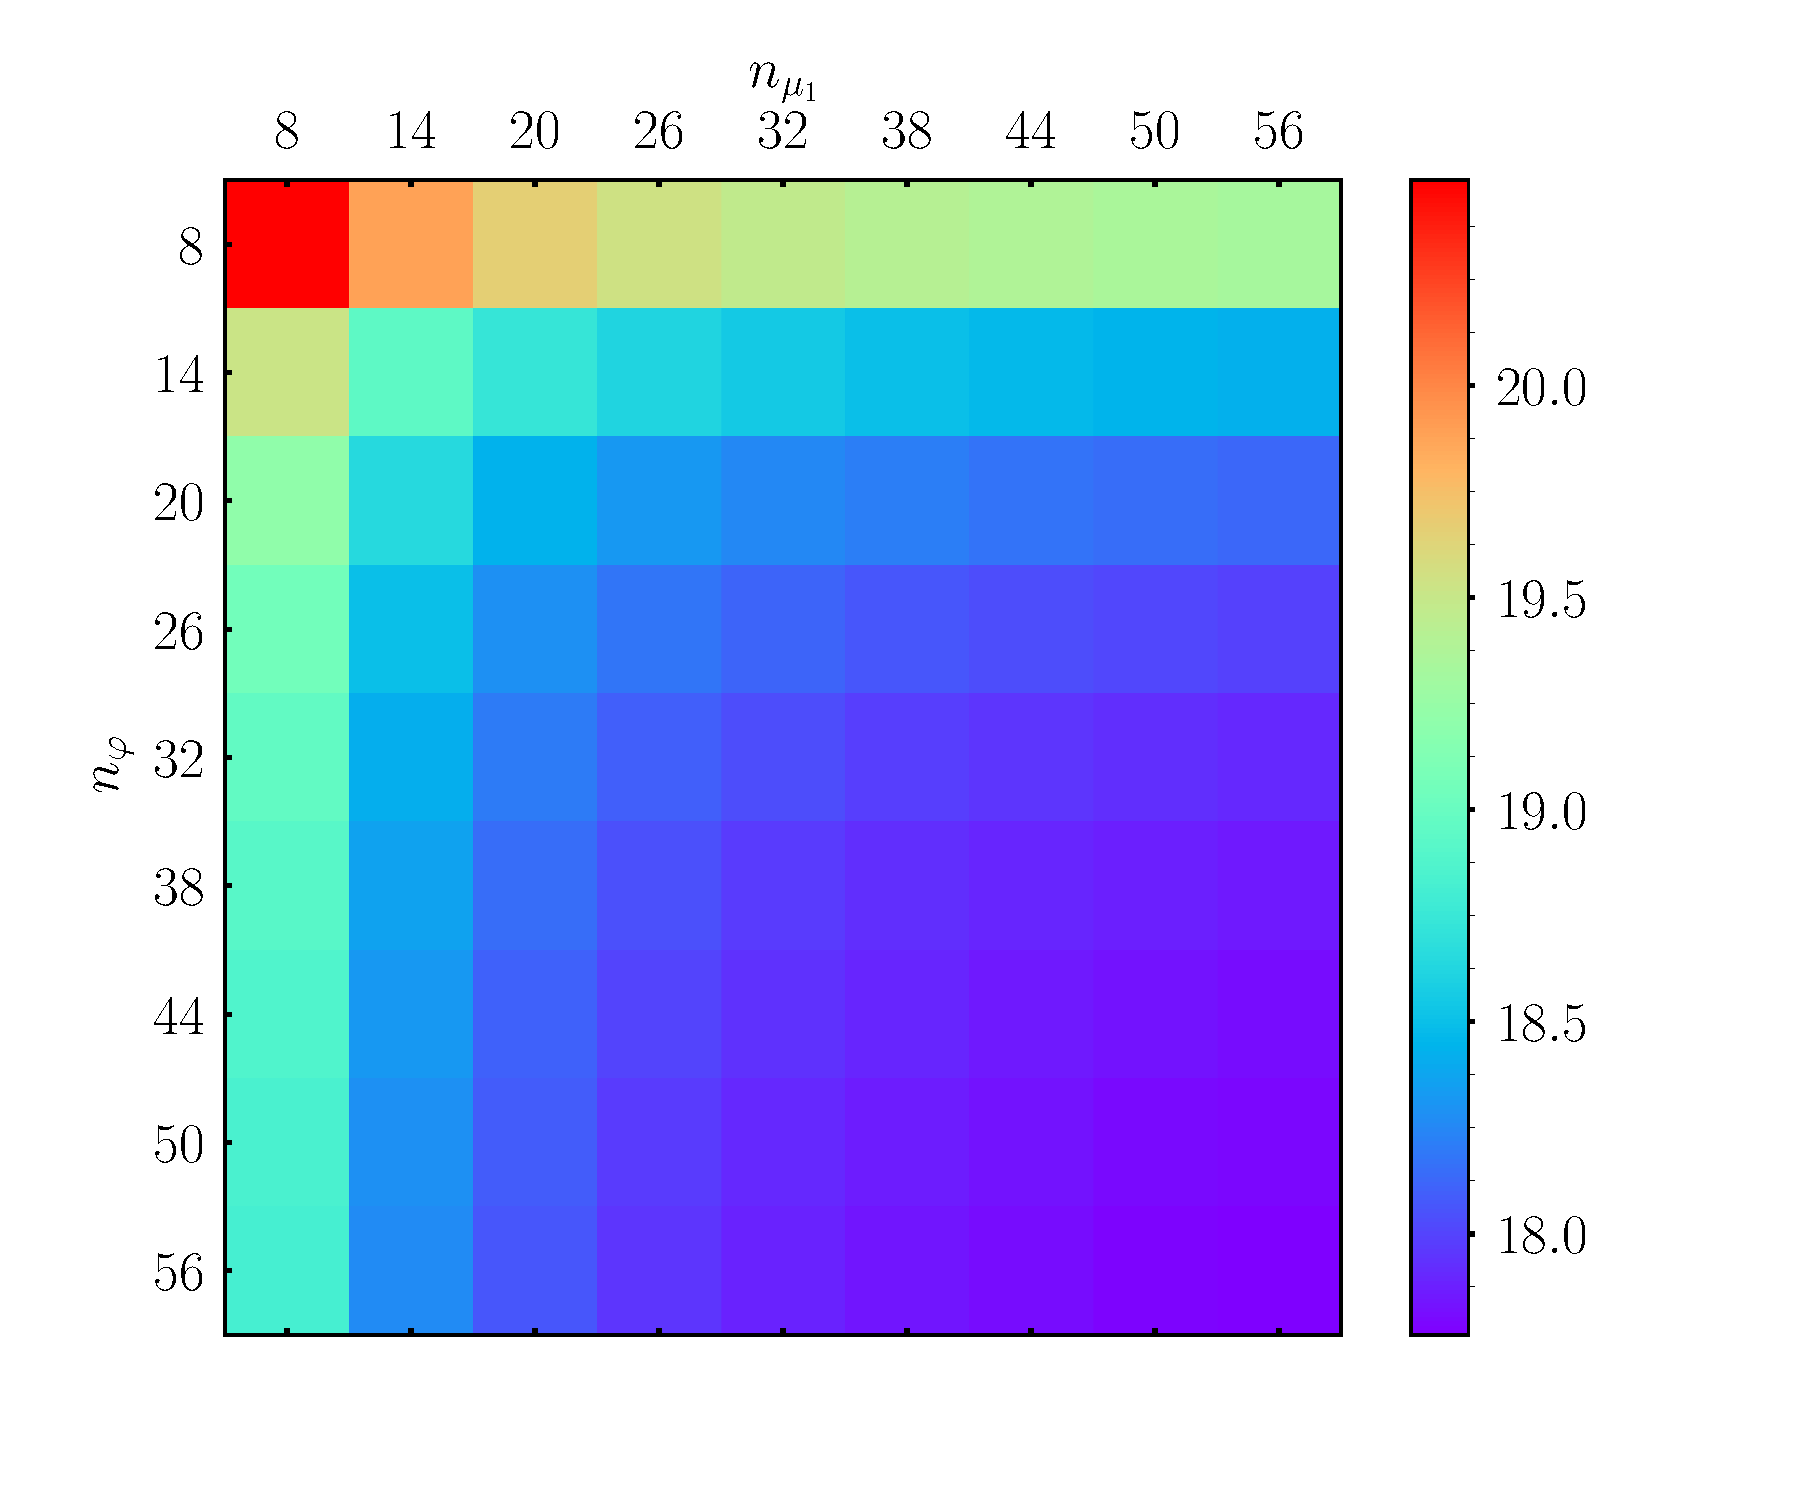
\includegraphics[width=8.0cm]{fig/colournmu1nphi_Doppler-eps-converted-to} 
\caption{Effect on 
{total} relativistic SNR of changing number of  $\varphi$ and $\mu_1$ bins. 
} \label{fig4x}
\end{figure} 


\subsection*{{Effect of changing magnification and evolution biases}}

The effect on the relativistic SNR of changes in magnification bias and in evolution bias is illustrated in Fig.~\ref{fig1x}.

\begin{figure}[ht]
\centering
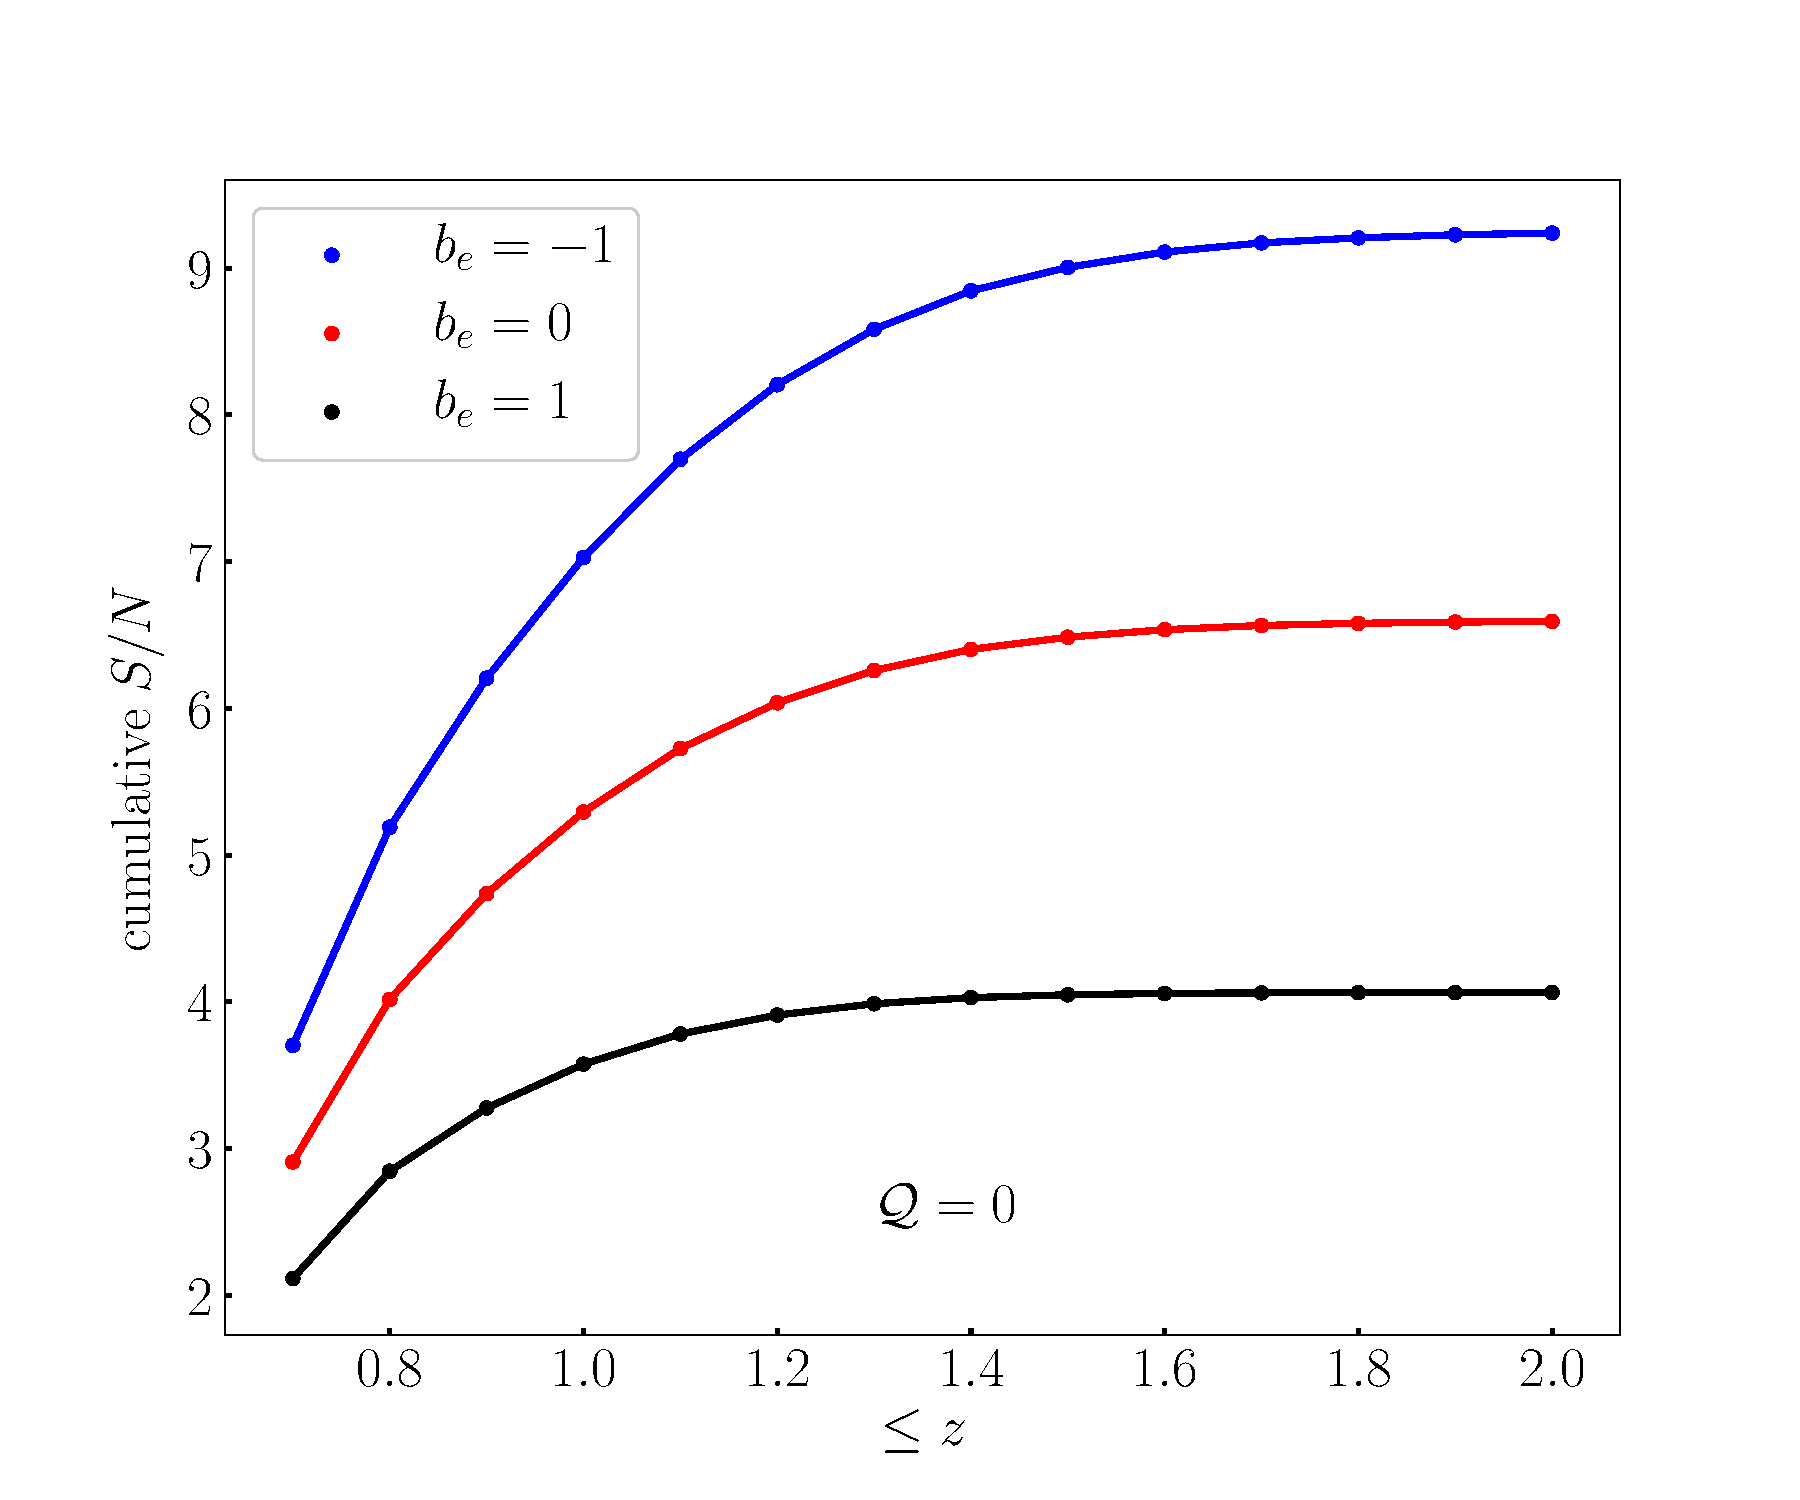
\includegraphics[width=7cm]{fig/cumulativeSnrdopplerQ0_0-eps-converted-to} 
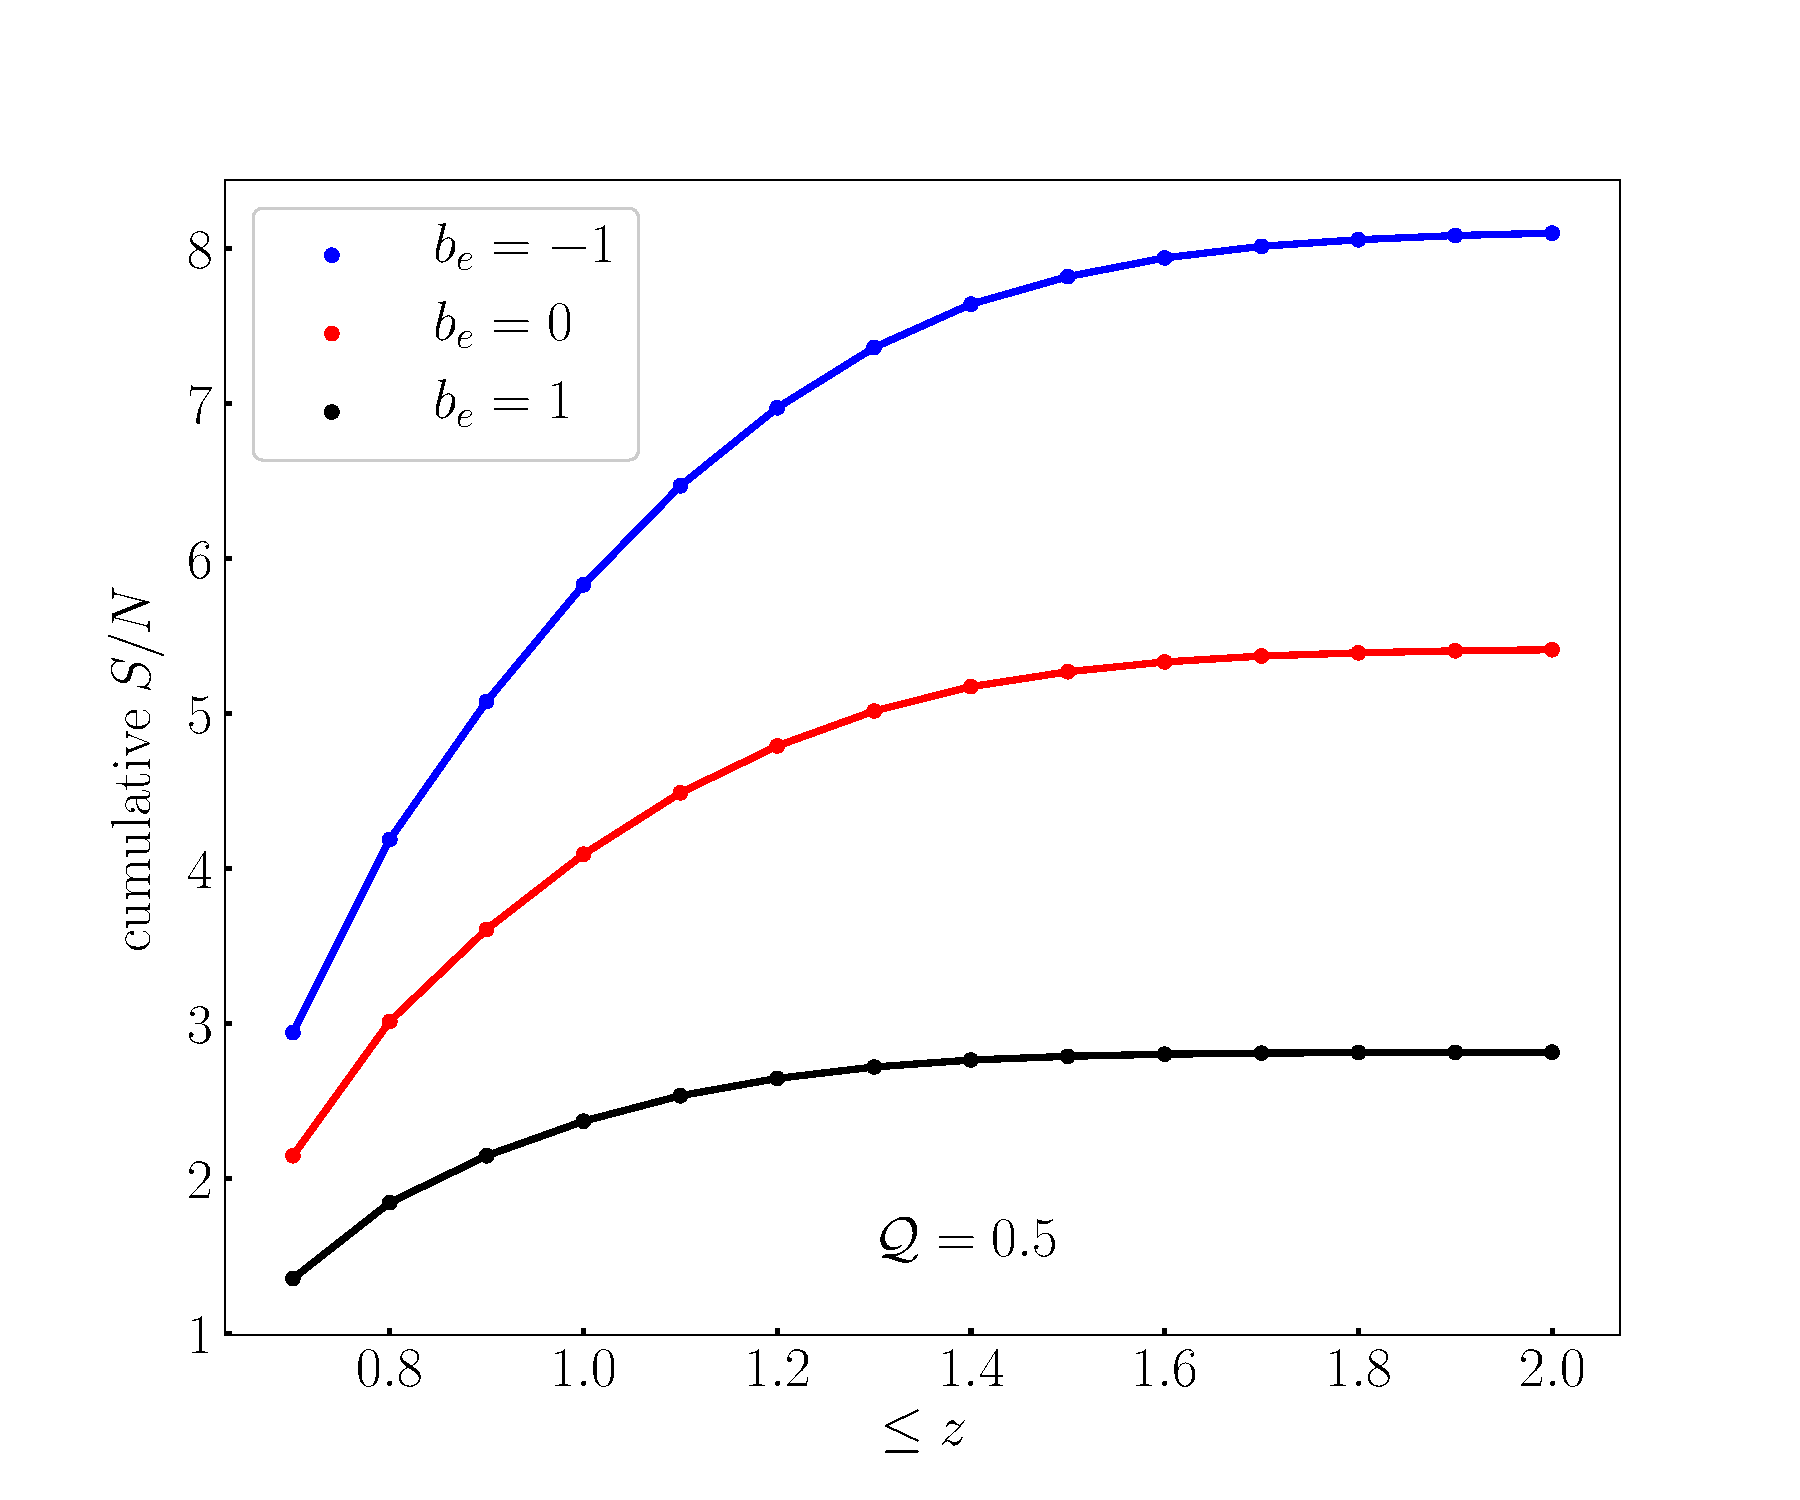
\includegraphics[width=7cm]{fig/cumulativeSnrdopplerQ0_5-eps-converted-to} \\
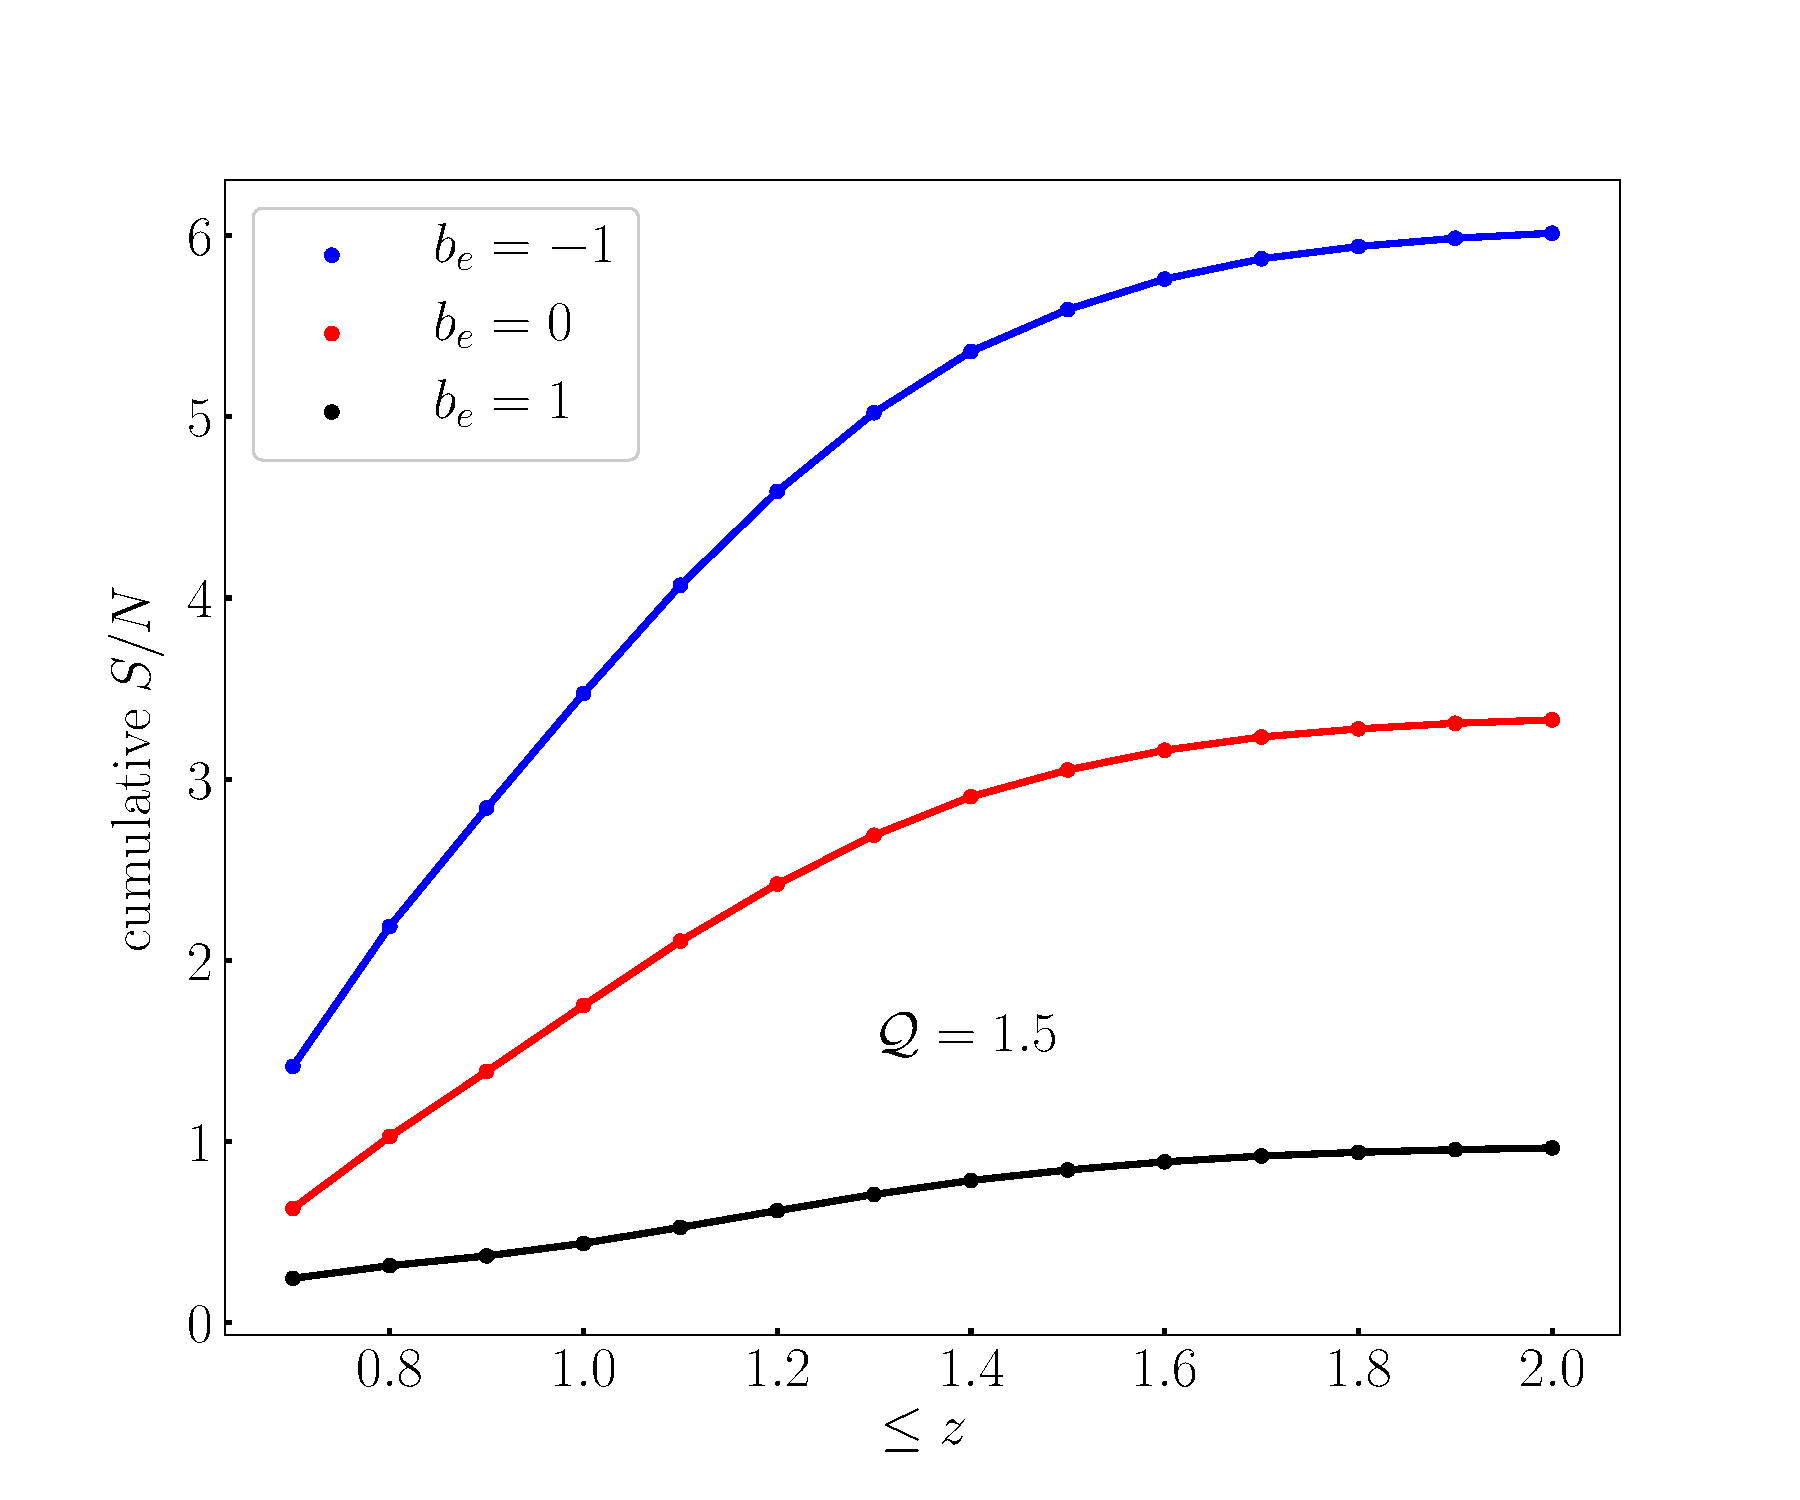
\includegraphics[width=7cm]{fig/cumulativeSnrdopplerQ1_5-eps-converted-to}
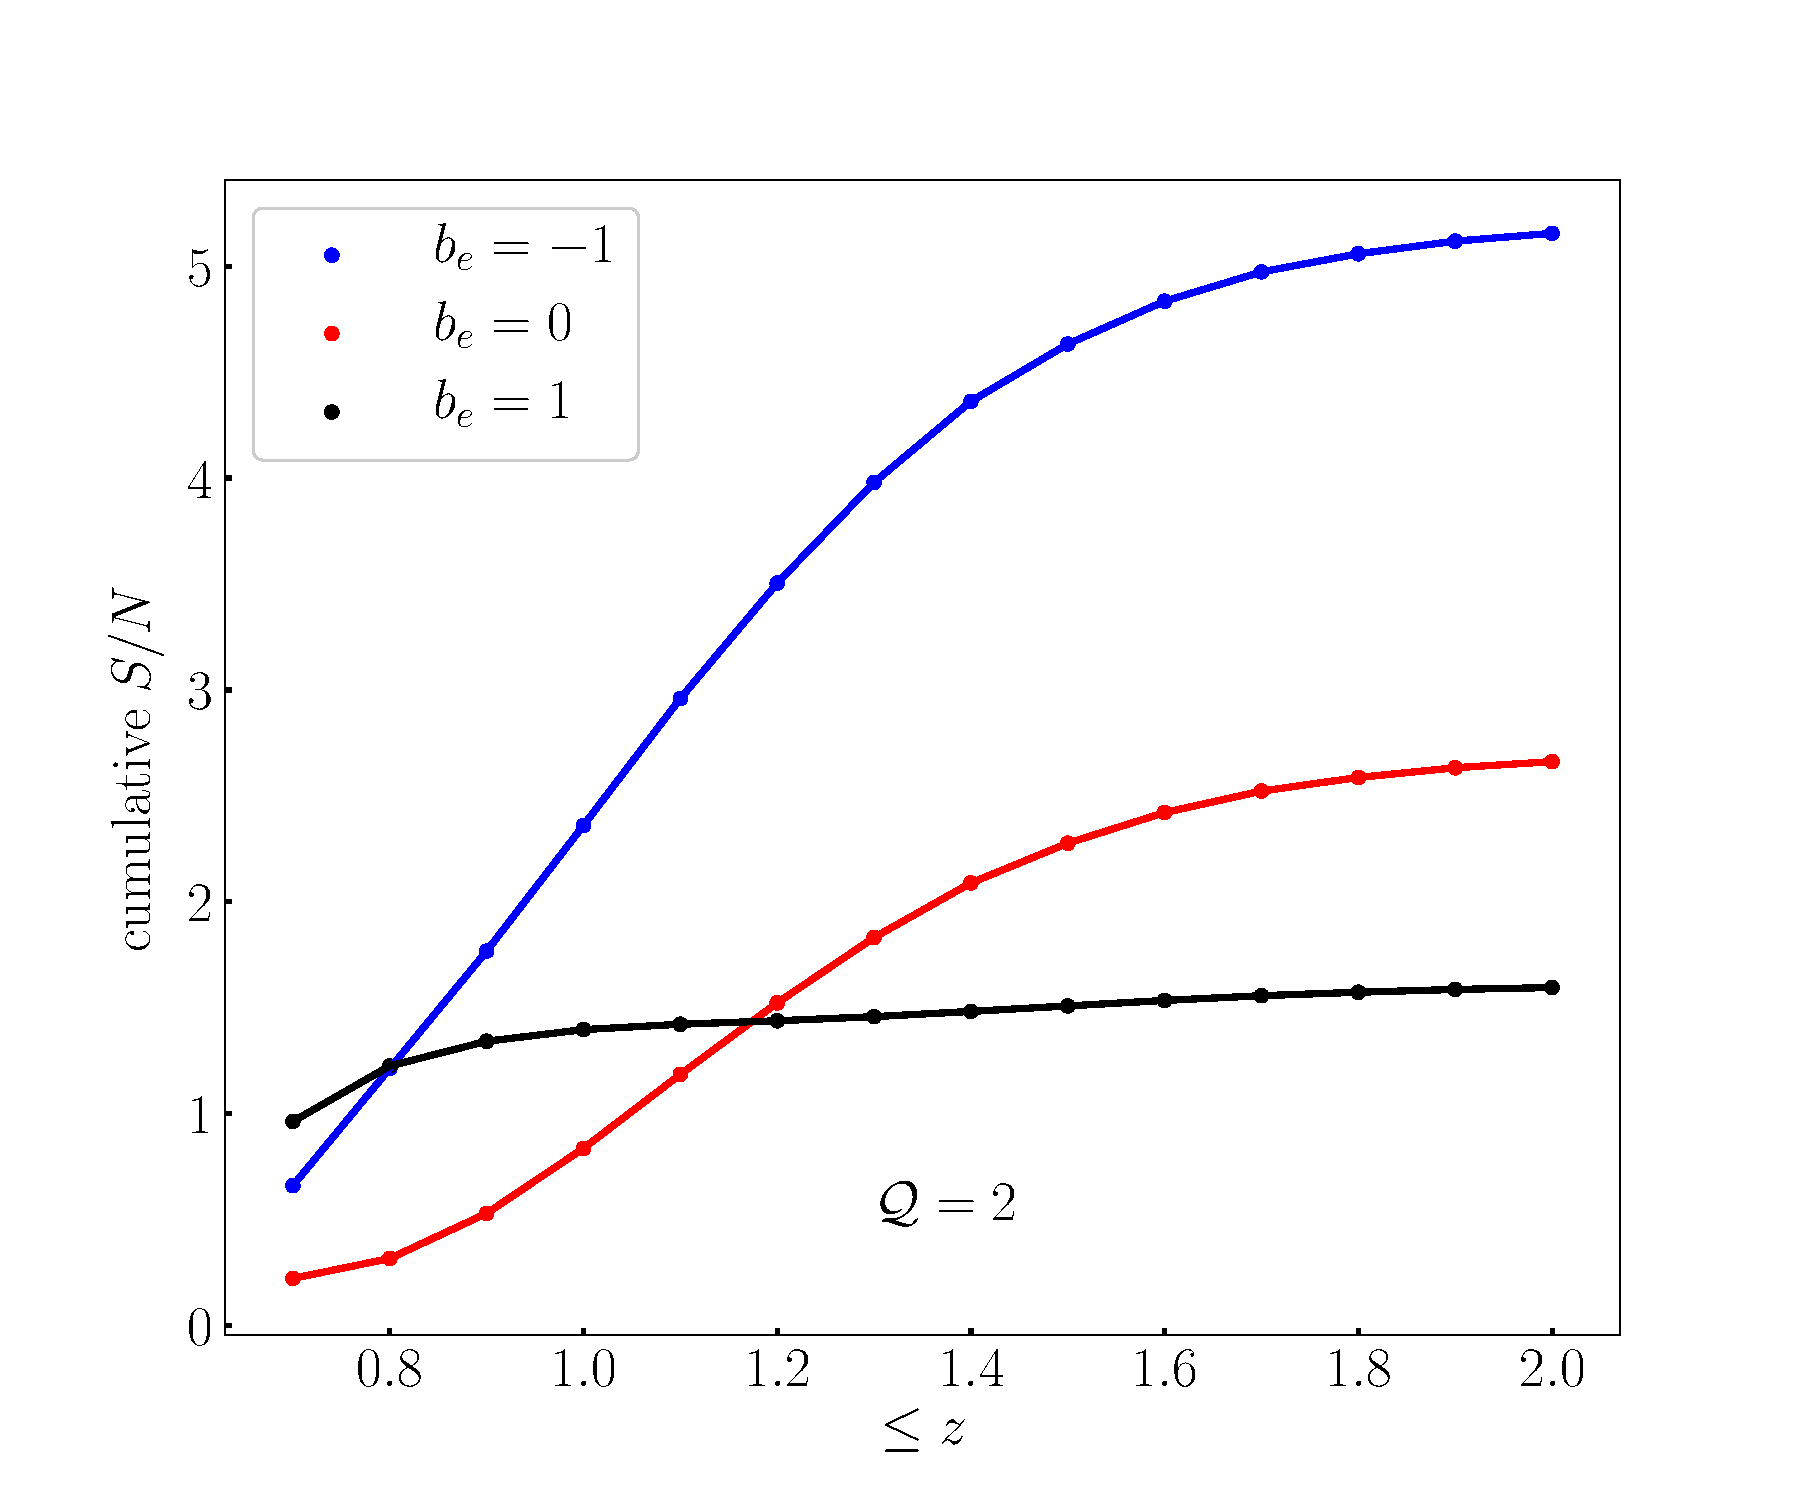
\includegraphics[width=7cm]{fig/cumulativeSnrdopplerQ2_0-eps-converted-to} 
\caption{Effect of changing ${\cal Q}$ and $b_e$ on relativistic cumulative SNR.} \label{fig1x}
\end{figure}


\subsection*{{Comparison with \cite{Jeong:2019igb}}}

In \cite{Jeong:2019igb},  
a significant number of terms is neglected in the relativistic second-order  galaxy number count contrast, $\delta_{g\mathrm{D}}^{(2)}$, given by our \eqref{dg2}. (Note that our  \eqref{dg2}, derived in \cite{Clarkson:2018dwn}, was independently confirmed by \cite{DiDio:2018zmk}). They have the first term, $A\, \bm{v}^{(2)}\!\!\cdot\bm{n}$, on the right of \eqref{dg2}.  In the second term, $2{C}(\bm{v}\cdot\bm{n})\,\delta$, they do not have the correct form of the coefficient $C$ -- they include only the first part, $b_1A$, of $C$ [see the right-hand side of eq 26?]. All terms after the second term in \eqref{dg2} are omitted by \cite{Jeong:2019igb}. Note that none of the omitted terms is suppressed by a higher power of $k^{-1}$;  they all have the same scaling, i.e., $\propto (\cH/k)\,{(\delta)^2}$. In detail, they omit the following
terms:
\begin{align}
\delta_{g\mathrm{D}}^{(2)}({\mathrm{us}})- \delta_{g\mathrm{D}}^{(2)}(\mbox{{\cite{Jeong:2019igb}}}) &= 2\left[b_{1}f + \frac{b_1'}{\cH} 
+ 2\bigg(1-\frac{1}{{r} \cH}\bigg){\frac{\partial b_1}{\partial \ln{L}}\bigg|_{\mathrm{c}}} \right](\bm{v}\cdot\bm{n})\,\delta 
\\\nonumber
& 
+ \frac{2}{\cH}\left(4-2A-\frac{3}{2}\Omega_{m} \right)(\bm{v}\cdot\bm{n})\,\partial_r(\bm{v}\cdot\bm{n})\\
\nonumber
&
+ \frac{2}{\cH^2}\big[(\bm{v}\cdot\bm{n}) \,\partial_r^2\Phi-\Phi\, \partial_r^2 (\bm{v}\cdot\bm{n}) \big]
 - \frac{2}{\cH}\,\partial_r (\bm{v}\cdot\bm{v}) + 2 \frac{b_1}{\cH}\,\Phi\, \partial_r\delta \,. 
\end{align}
%
% \chapter{HI intensity mapping}
% \label{app_im}
% %
% \section{HI bias parameters} \label{app1}

We follow \cite{Umeh:2015gza} to compute $b_{1}$ and $b_{2}$ from a halo-model approach:
\begin{align}
b_{1} &= 1 + \left\langle \frac{2p+\big(q\nu - 1\big)\big[1+(q\nu)^{p}\big]}{\delta_{\rm cr}\big[1+(q\nu)^{p}\big]} \right\rangle _{\!\!\!\rm m}  \!\!, \label{e1.16} \\
b_{2} &= \frac{8}{21}\big(b_{1}-1\big) + \left \langle \frac{2p\big(2p+2\nu q-1\big)+ q\nu\big(q\nu-3\big)\big[1+(q\nu)^{p}\big]}{\delta_{\rm cr}^{2}\big[1+(q\nu)^{p}\big]}  \right \rangle _{\!\!\!\rm m}  \!\!, \label{e1.17}
\end{align}
where the parameters $p$, $q$ and $\nu$ are related to the Sheth-Tormen distribution function (see \cite{Sheth:1999su, Sheth:2001dp, Sheth:1999mn} for more details), and $\delta_{\rm cr}$ is the critical density at which halos collapse spherically \cite{Kitayama:1996ne}, 
\begin{equation}
\delta_{\rm c}(z) = \frac{3(12\pi)^{2/3}}{20}\big[1+0.0123\log{\Omega_{\rm m} (z)}\big] \,. \label{e1.20}
\end{equation}
The mass average is defined by 
\begin{equation}
\big\langle X_{h}(z,\bm{x}) \big\rangle _{\rm m}  = \frac{\int_{M_{-}}^{M_{+}} \ud M\,X_{h}(z,\bm{x},M)\,M_{\mathrm{HI}}(M)\,n_{h}(z,\bm{x},M)}{\int_{M_{-}}^{M_{+}} \ud M\,M_{\mathrm{HI}}(M)\,n_{h}(z,\bm{x},M)} \, , \label{e1.18}
\end{equation}
where $M$ is the mass of {halos} that can host HI gas, and $M_{\pm}$ are the lower and upper mass limits, which are  related to the circular velocities  of the galaxies \citep{Bull:2014rha}. $n_{h}$ is the halo mass function \citep{Sheth:1999su, Sheth:2001dp,Tellarini:2015faa}, and $M_{\rm HI}$ is the HI mass function, which is assumed to follow a power law  \citep{Santos:2015gra},
\begin{equation}
M_{\mathrm{HI}}(M) \propto M^{0.6} \,. \label{e1.19}
\end{equation}
 Figure~\ref{fig1} shows the numerical results from \eqref{e1.16} and \eqref{e1.17}. Fitting formulas for the bias parameters are
\bea
b_{1}(z)& = & 0.754 + 0.0877z + 0.0607z^{2} - 0.00274z^{3}\,, \label{e1.27} \\
b_{2}(z) &= & -0.308 - 0.0724z - 0.0534z^{2} + 0.0247z^{3}\,. \label{e1.28}
\eea
Assuming that  halo formation is a local process in Lagrangian space and that there is no initial tidal bias, the tidal bias is \cite{Tellarini:2015faa}:
\begin{equation}
b_{s^{2}} = \frac{4}{7}\big(1-b_{1}\big)\,.\label{e1.21} 
\end{equation} 

\clearpage

\section{MeerKAT and SKA system temperatures} \label{app2}
\vspace*{-0.5cm}
\begin{table}[! ht]
\centering
\caption{\label{tab5} System temperatures for MeerKAT and SKA1-MID, used in Figure~\ref{fig2} (from \cite{Fonseca:2019qek}).} 
\vspace*{0.2cm}
  \begin{tabular}{|l|l|l|l|l|l|l|l|}
    \hline
      \multicolumn{2}{|c|}{MeerKAT L Band} &
      \multicolumn{2}{c|}{MeerKAT UHF Band} &
      \multicolumn{2}{c|}{SKA1-MID Band 1} & 
      \multicolumn{2}{c|}{SKA1-MID Band 2} \\
      \hline \hline
    $~~~~z~~$ & $~~T_{\rm sys}\;/\;\rm K~~~$ & $~~~z~$ & $~~~~T_{\rm sys}\;/\;\rm K~~$ & $~~~z~$ & $~~T_{\rm sys}\;/\;\rm K~~$ & $~~~~z~~$ & $~~T_{\rm sys}\;/\;\rm K~~$ \\
    \hline
    
  %& & & & & & & \\
  
     0.136 & ~~~~19.2 & 0.420 & ~~~~~~20.3 & 0.403 & ~~~~27.2 & 0.115 & ~~~~16.4 \\
    
     0.183 & ~~~~19.7 & 0.495 & ~~~~~~21.0 & 0.470 & ~~~~26.9 & 0.168 & ~~~~16.6 \\
    
     0.235 & ~~~~20.3 & 0.578 & ~~~~~~21.7 & 0.539 & ~~~~26.8 & 0.223 & ~~~~16.8 \\
    
     0.291 & ~~~~20.9 & 0.671 & ~~~~~~22.5 & 0.612 & ~~~~26.9 & 0.280 & ~~~~17.0 \\
    
     0.352 & ~~~~21.5 & 0.775 & ~~~~~~23.5 & 0.767 & ~~~~27.5 & 0.341 & ~~~~17.2 \\
    
    0.420 & ~~~~22.3 & 0.893 & ~~~~~~24.7  & 0.850 & ~~~~28.1 & 0.403 & ~~~~17.6 \\
    
    0.495 & ~~~~23.1 & 1.03 & ~~~~~~26.1   & 0.938 & ~~~~28.8 & 0.470  & ~~~~18.0 \\
    
    0.578 & ~~~~24.0 & 1.18 & ~~~~~~27.9   & 1.03  & ~~~~29.8 &        &  \\
    
          &          & 1.37 & ~~~~~~30.3   & 1.12  & ~~~~30.8 &        &  \\
     
          &          & 1.45 & ~~~~~~31.5   & 1.22  & ~~~~32.1 &        &  \\
    
          &          &      &              & 1.33  & ~~~~33.5 &        &   \\
    
          &          &      &              & 1.44  & ~~~~35.2 &        &    \\
    
          &          &      &              & 1.55  & ~~~~37.1 &        &   \\
    
          &          &      &              & 1.67  & ~~~~39.2 &        &   \\
    
          &          &      &              & 1.80  & ~~~~41.6 &        & \\
    
          &          &      &              & 1.93  & ~~~~44.2 &        &  \\
    
          &          &      &              & 2.07  & ~~~~47.2 &        &  \\
    
          &          &      &              & 2.22  & ~~~~50.6 &        &  \\
    
          &          &      &              & 2.37  & ~~~~54.4 &        &  \\
    
          &          &      &              & 2.54  & ~~~~58.6 &        &  \\
    
          &          &      &              & 2.69  & ~~~~63.4 &        &  \\
    
          &          &      &              & 2.87  & ~~~~68.8 &        &  \\
    
          &          &      &              & 3.05  & ~~~~74.8 &        &  \\
    
 %         &          &      &              &       &          &        &  \\
    \hline
  \end{tabular}
\end{table}
\vspace*{-0.5cm}
 \begin{figure}[! h]
\centering
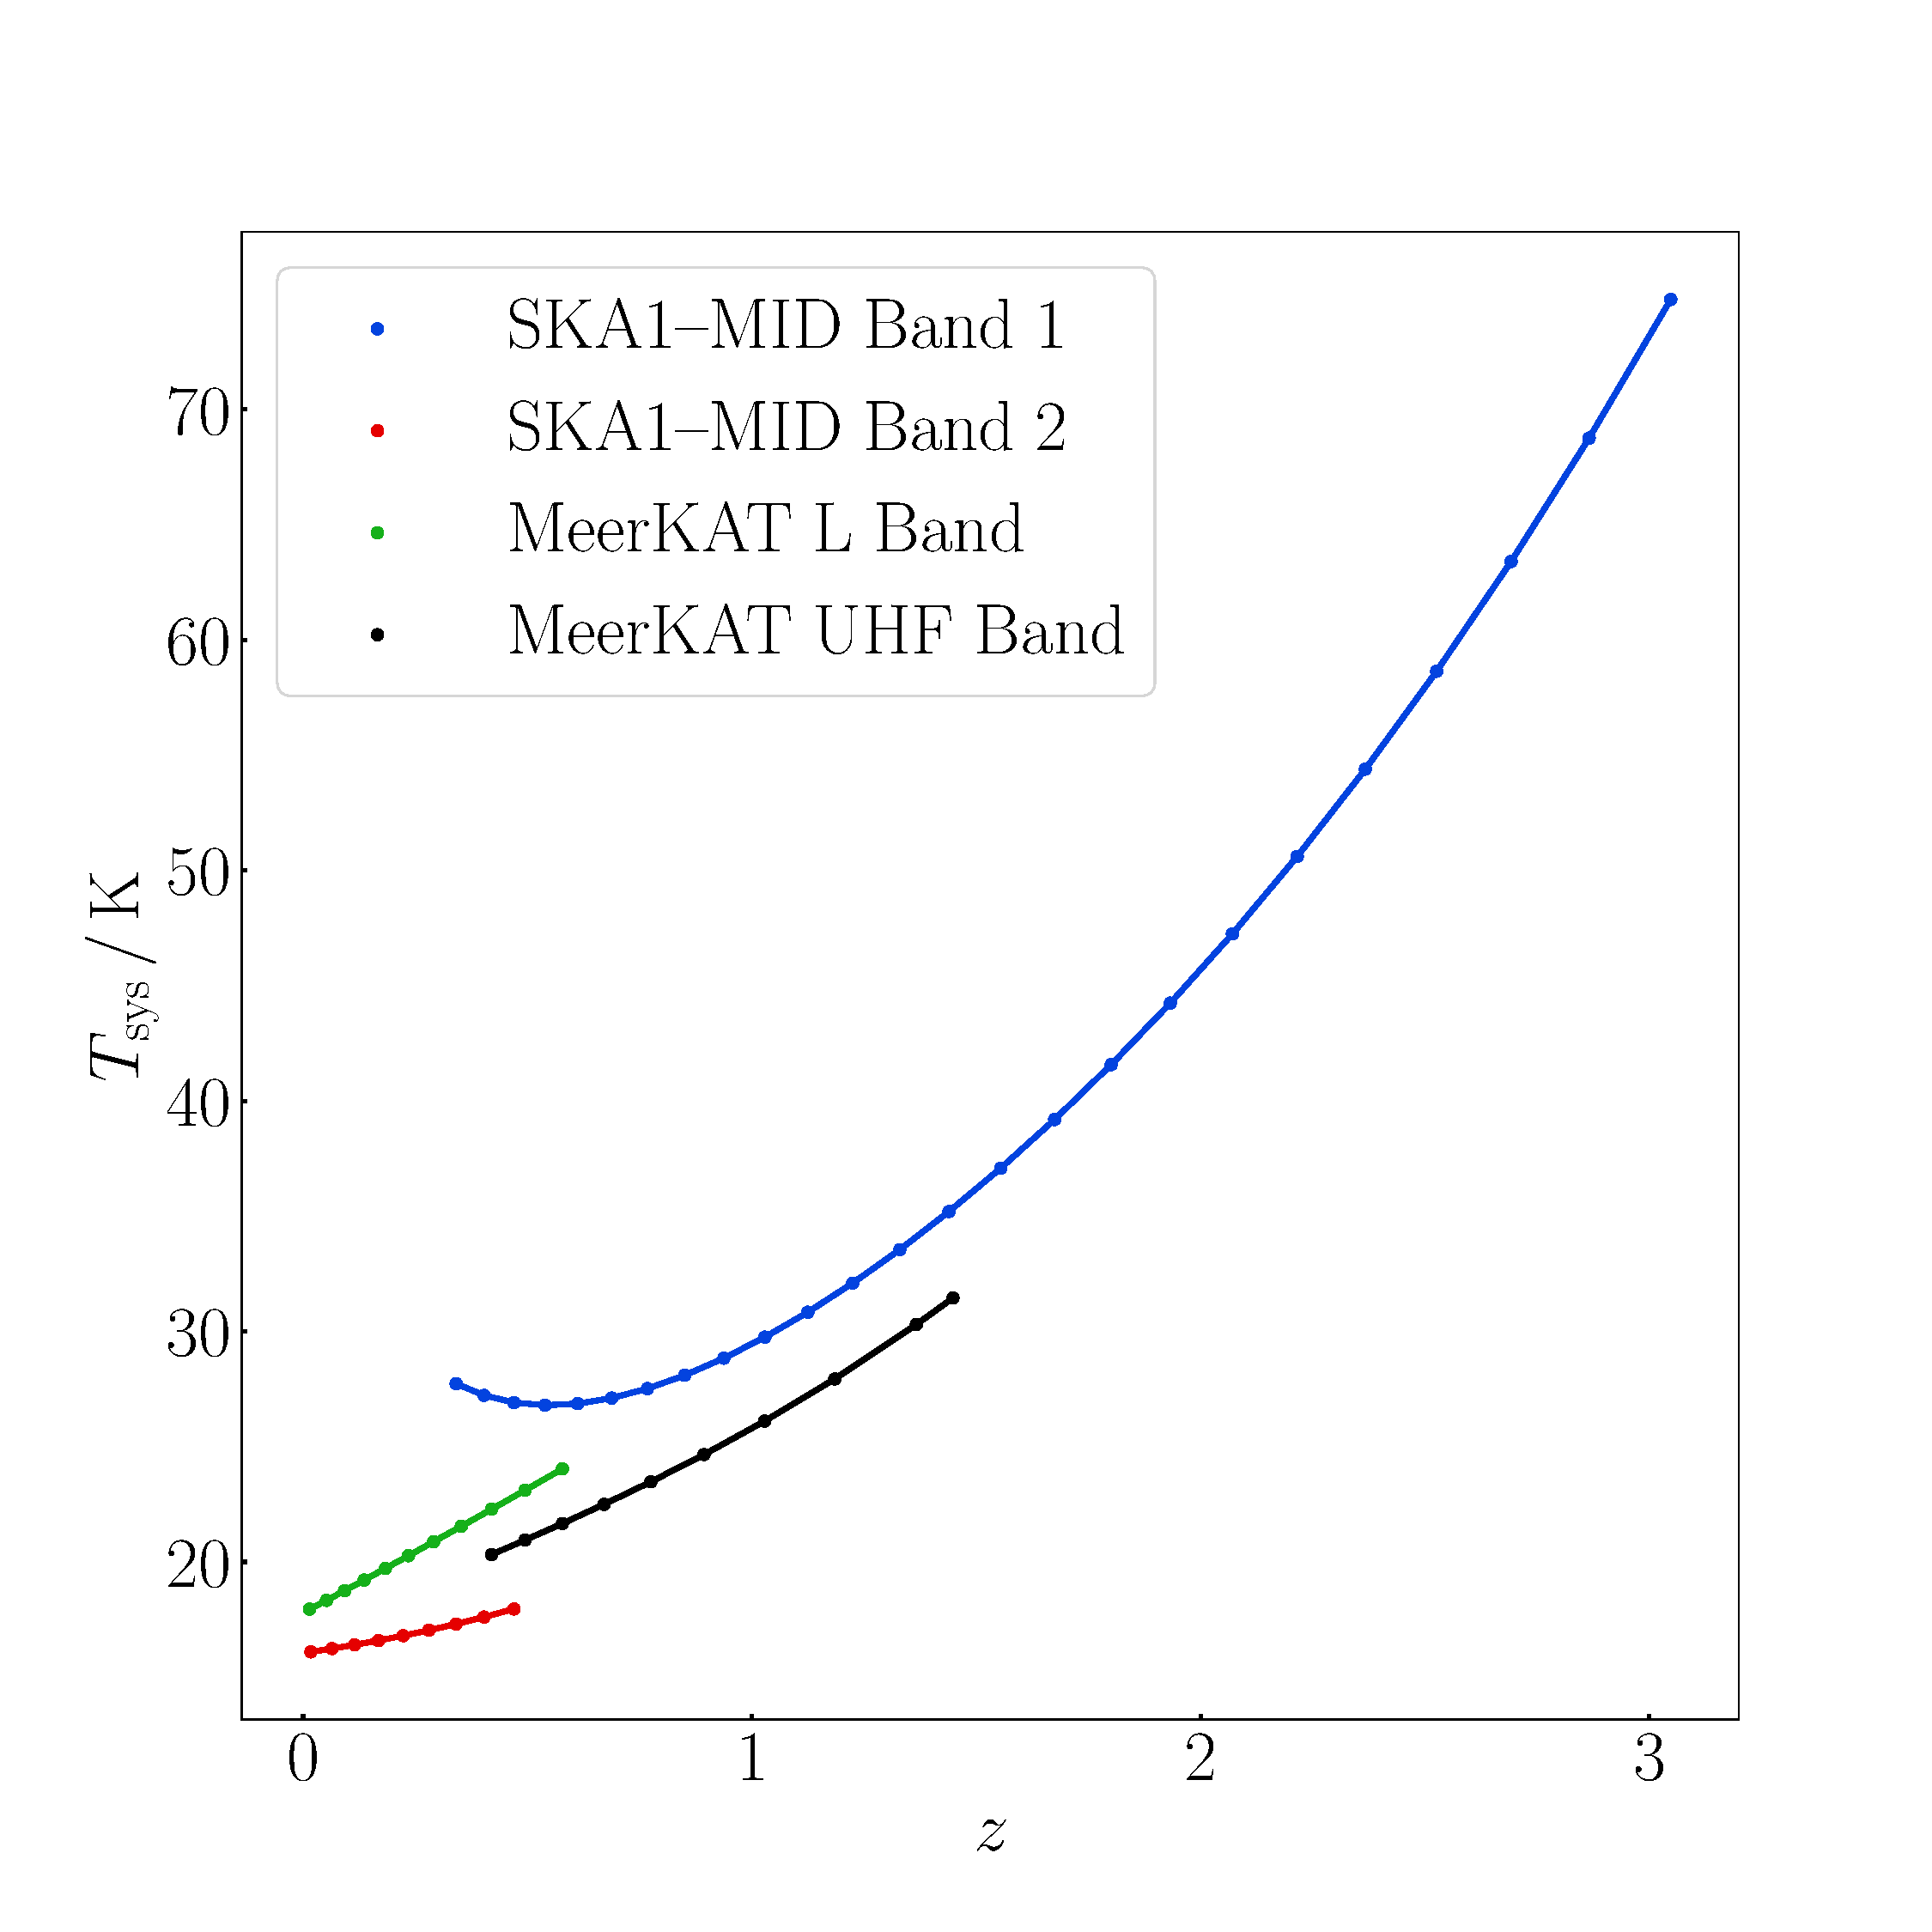
\includegraphics[width=.49\textwidth]{tSys}
\vspace*{-0.5cm}
\caption{$T_{\rm sys}$ for the different frequency bands of MeerKAT and SKA1 (from Table \ref{tab5}).} \label{fig2}
\end{figure}
%
\end{appendices}


% % % % % % % % % % % % % % % % % % % % % % % % % % 
% Start single space again for bibliography
\begin{singlespace}
% % % % % % % % % % % % % % % % % % % % % % % % % 

% Bibliography
% Put your bibliography file here
\bibliography{bib/thesis_bib}
% 
% This bibtex style file puts entries in alphabetical order and treats arxiv
% references correctly.
%\bibliographystyle{abbrvnat}
%\bibliographystyle{unsrt}
%\bibliographystyle{./utphys-ih}
%\bibliographystyle{ieeetr} %cth one I found in order of appearence
%\bibliographystyle{plainnat}


% % % % % % % % % % % % % % % % % % % % % % % % % 

\end{singlespace}

\listoffigures 
\listoftables 


% % % % % % % % % % % % % % % % % % % % % % % % % 
\end{document}
